\documentclass[twoside,openright]{iitdhthesis}
\usepackage{packages}

\usepackage{graphicx}
\usepackage{times}
\usepackage{cite}
\usepackage{url}
%\usepackage[linktocpage]{hyperref}
\usepackage[english]{babel}
% \usepackage[inline]{showlabels}%used to display the labels of environments. Inline option shows alongside.
\usepackage[acronym,nonumberlist,sort=use]{glossaries}
\usepackage{emptypage}
\usepackage{verbatim}
\usepackage{tikz}
\usetikzlibrary{arrows,automata}
\tikzset{every state/.style={minimum size=0pt}}


\setcounter{topnumber}{4}              %max floats in top half
\setcounter{bottomnumber}{4}           %max floats in bottom half
\setcounter{totalnumber}{4}            %max floats per page
\renewcommand{\topfraction}{0.9}       %max fraction of top half for floats
\renewcommand{\bottomfraction}{0.9}    %max fraction of bottom half for floats
\renewcommand{\textfraction}{0.1}      %min text fraction on a page

\pdfinfo{
   /Author (Author name)
   /Title  (PhD Thesis)
   /Subject (Thesis title)
}
\newglossaryentry{ModelChecking}{
    type=main,
    name=Model Checking,
    description={Model checking is a formal  verification technique which allows for desired behavioral properties of a given system to be verified on the basis of a suitable model of the system through systematic inspection of all states of the model}}


\newglossaryentry{SymbolicModelChecking}{
    type=main,
    name=Symbolic Model Checking,
    description={Symbolic model checking is a methodology where instead of explicitly checking all the states of the system, symbolic model checking algorithms manipulate sets of states}
}

\newglossaryentry{PetriNet}{
    type=main,
    name=Petri Net,
    description={A Petri net is a mathematical modeling tool used to simulate and analyze systems that involve concurrency, synchronization, and resource sharing}
}

\newglossaryentry{Formalverification}{
    type=main,
    name=Formal verification,
    description={Formal verification is the act of proving or disproving the correctness of a system with respect to a certain formal specification or property}}

\newglossaryentry{symb:nu}{
    type=symbols,
    name=$\nu$,
    description={Variable used to denote the newly created identifiable token}
}

\newglossaryentry{symb:kappa}{
    type=symbols,
    name=$\kappa$,
    description={Variable used to denote the number of clients
            which currently are in a given local state}
}

\newglossaryentry{symb:lambda}{
    type=symbols,
    name=\ensuremath{\lambda},
    description={Variable used to denote the execution step}
}

\newglossaryentry{symb:alpha}{
    type=symbols,
    name=$\alpha$,
    description=The temporal property that is being verified}

\newacronym{BMC}{BMC}{Bounded Model Checking}

\newacronym{BA}{BA}{B{\"u}chi automata}

\newacronym{PN}{PN}{Petri nets}

\newacronym{WPN}{WPN}{Weighted Petri nets}

\newacronym{APS}{APS}{Autonomous Parking System}

\newacronym{MCC}{MCC}{Model Checking Contest}

\newacronym{XML}{XML}{Extensible Markup Language}

\newacronym{PNML}{PNML}{Petri Net Markup Language}

\newacronym{LTL}{LTL}{Linear Temporal Logic}

\newacronym{CTL}{CTL}{Computation Temporal Logic}

\newacronym{MFOTL}{MFOTL}{Monadic First Order Temporal Logic}

\newacronym{ANTLR}{ANTLR}{ANother Tool for Language Recognition}

\newacronym{FOL}{FOL}{First Order Logic}

\newacronym{NNF}{NNF}{Negation Normal Form}

\newacronym{LP}{LP}{Logic Program}

\newacronym{ASP}{ASP}{Answer Set Programming}
\makeglossaries

\newglossarystyle{custom_acronyms}{%
  \setglossarystyle{super}% base style on the list style
  \renewenvironment{theglossary}%
      {\tablehead{}\tabletail{}%
       \begin{supertabular}{lp{\glsdescwidth}}}%
      {\end{supertabular}}%
}

\begin{document}
% \newcommand{\Lstar}{$\mathsf{UCSTL}$}
\newcommand{\Lstar}{$\mathsf{FOTL_1}$}
%
\newtheorem{dfn}{Definition}[section]
\newtheorem{prop}[dfn]{Proposition}
\newtheorem{lem}[dfn]{Lemma}
\newtheorem{thm}[dfn]{Theorem}
\newtheorem{cor}[dfn]{Corollary}
\newtheorem{eg}[dfn]{Example}
\theoremstyle{remark}
\newtheorem{remark}{Remark}

\newcommand\beq{\begin{equation}}
\newcommand\enq{\end{equation}}


\newcommand{\LC}{$LTL_{LIA}$}

%
\newcommand{\RightBox}{{\phantom{a}}\hfill $\Box$ \\}
\newenvironment{prf}{{\bf Proof~Idea:~}}{\RightBox}

%
\newcommand{\Dfn}[1]{Definition \ref{dfn:#1}}
\newcommand{\Prop}[1]{Proposition \ref{prop:#1}}
\newcommand{\Lem}[1]{Lemma \ref{lem:#1}}
\newcommand{\Thm}[1]{Theorem \ref{thm:#1}}
\newcommand{\Cor}[1]{Corollary \ref{cor:#1}}

%Action-indexed diamond modality
\newcommand{\Adiam}[1]{\mbox{$\langle #1 \rangle$}}
\newcommand{\diamin}{\Diamond\kern-0.5em{\raisebox{.25ex}{\rm -}}\kern0.175em}
\newcommand{\until}{\mbox{\large\bf U}}
\newcommand{\since}{\mbox{\large\bf S}}
\newcommand{\nxt}{\mbox{$\bigcirc$}}
\newcommand{\nxtdot}{\displaystyle \bigodot}
\newcommand{\past}{\diamin}
\newcommand{\ifpast}{\mbox{$\boxminus$}}
\newcommand{\now}{\mbox{$\langle now \rangle$}}
\newcommand{\Now}{\mbox{$[now]$}}
\newcommand{\pres}{\mbox{$\rangle \langle$}}
\newcommand{\snd}{\mbox{\large\bf s}}
\newcommand{\rec}{\mbox{\large\bf r}}
\newcommand{\nc}{\mathbf{no\_comm}}

%Propositional connectives
%\newcommand{\implies}{{\raisebox{.20ex}{$\scriptstyle ~\supset~$}}}
\newcommand{\Not}{\mbox{$\lnot$}}
\newcommand{\xor}{\oplus}
\newcommand{\True}{\mathit{True}}
\newcommand{\False}{\mathit{False}}
\newcommand{\Imply}{\supset}
%Large symbols
\newcommand{\andover}{\displaystyle \bigwedge}
\newcommand{\orover}{\displaystyle \bigvee}
\newcommand{\capover}{\displaystyle \bigcap}
\newcommand{\cupover}{\displaystyle \bigcup}
\newcommand{\piover}{\displaystyle \Pi}
\newcommand{\ohat}[1]{\widehat{#1}}
\newcommand{\otilde}[1]{\widetilde{#1}}
\newcommand{\obar}[1]{\overline{#1}}
\newcommand{\Sigtil}{\mbox{$\otilde{\Sigma}$}}
\newcommand{\DA}{\mbox{$\Sigtil~=~(\Sigma_1, \dots, \Sigma_n)$}}

%Useful symbols
\newcommand{\derives}{\vdash}
\newcommand{\defn}{\mbox{$~\stackrel{\rm def}{=}~$}}
\newcommand{\qneq}{\mbox{$~\stackrel{\rm ?}{=}~$}}
\newcommand{\eqv}{\approx}
% \newcommand{\hash}{\sharp}
\newcommand{\restr}{\lceil}
%\newcommand{\bot}{\bottom}
\newcommand{\nat}{{\bf N}}
\newcommand{\pfin}[1]{\mbox{$\wp_{fin}(#1)$}}
%\newcommand{\mod}[1]{\mbox{$|#1|$}}
\newcommand{\memb}[2]{\mbox{${#1} \in {#2}$}}
\newcommand{\E}{\mathbf{E}}



%Some roman words in math mode
\newcommand{\Iff}{\mbox{~iff~}}
%\newcommand{\For}{\mbox{~for~}}
\newcommand{\Where}{\mbox{~where~}}
%\newcommand{\And}{\mbox{~and~}}
\newcommand{\Implies}{\mbox{~implies~}}

% structures
\newcommand{\Sigstr}{\mbox{$\Sigma^*$}}
% \newcommand{\TS}{\mbox{$TS = (Q,\to)$}}  %generates TS=(Q,->)

% classes
\newcommand{\mdl}[1]{\mbox{${\cal M}_{#1}$}}%generates script M with subscript
\newcommand{\dmodels}{\mbox{$\models_{Det}~$}}

% For transitions steps
\newcommand{\step}[1]{\mbox{$\stackrel{#1}{\to}$}}
\newcommand{\squigto}{\rightsquigarrow}
\newcommand{\longstep}[1]{\mbox{$\stackrel{#1}{\longrightarrow}$}}
\newcommand{\emptystep}{\step{\emptyset}}
% \newcommand{\reach}[1]{\mbox{${\cal R}(#1)$}}
% \newcommand{\reachin}[2]{\mbox{${\cal R}_{#1}(#2)$}}

% For a "double-lined" transition relation
\newcommand{\To}{\Rightarrow}
\newcommand{\From}{\Leftarrow}
\newcommand{\Step}[1]{\mbox{$\stackrel{#1}{\To}$}}
\newcommand{\Longstep}[1]{\mbox{$\stackrel{#1}{\Longrightarrow}$}}
\newcommand{\Longlongstep}[1]{\mbox{$\stackrel{#1}{\Longlongrightarrow}$}}
\newcommand{\Emptystep}{\Step{\emptyset}}

% Net theory
\newcommand{\presca}[1]{\mbox{${ }^{\bullet}#1$}}
\newcommand{\postsca}[1]{\mbox{$#1 \, { }^{\bullet}$}}%

%space optimization

\newcommand{\ldot}{{\rm <}\kern-0.37em{\raisebox{.25ex}{\bf .}}\kern0.375em}

\newcommand{\fmset}[1]{\{\{#1\}\}}


% \usepackage{todonotes}
% \usepackage{amsfonts}
% \usepackage{amsmath}
% \usepackage{amssymb}
% \usepackage{amsthm}
%\newcommand{\fmset}[1]{\{\{#1\}\}} %commented out
%%
%% One can fix some overfulls
% \sloppy

%%
%% Minted listings support 
%% Need pygment <http://pygments.org/> <http://pypi.python.org/pypi/Pygments>
%\usepackage{minted}
%% auto break lines
%\setminted{breaklines=true}





% \usepackage{amsmath}
% \usepackage{amsfonts}
% \usepackage{amssymb}
% \usepackage{amsthm}
% \usepackage{caption}
% \usepackage{subcaption}
% \usepackage{multirow}
% \usepackage{hyperref}
% \usepackage{paralist}

\theoremstyle{plain}
\newtheorem{theorem}{Theorem}
\newtheorem{proposition}{Proposition}
\newtheorem{corollary}{Corollary}
\newtheorem{conjecture}{Conjecture}
\newtheorem{lemma}{Lemma}
\theoremstyle{remark}
\newtheorem{example}{Example}
\theoremstyle{definition}
\newtheorem{definition}{Definition}

% \usepackage{paralist}

\newcommand{\multiset}[1]{\boldsymbol{#1}}
\newcommand{\rightmayr}{\xrightarrow[\text{Mayr}]}
\newcommand{\predecessor}{\mathit{Pred}}
\newcommand{\os}{\ensuremath{\mathfrak{E}}}
%\newcommand{\tup}[1]{\left\langle#1\right\rangle}
\newcommand{\tup}[1]{\langle#1\rangle}
\newcommand{\id}{\mathit{id}}
\newcommand{\supp}{\mathit{supp}}
\newcommand{\resN}{\overline{N}}
\newcommand{\sqleq}{\sqsubseteq}
\newcommand{\sqgeq}{\sqsupseteq}
\newcommand{\sqg}{\sqsupset}
\newcommand{\sql}{\sqsubset}
\newcommand{\reach}{\ensuremath{\mathit{Reach}}}
\newcommand{\cover}{\ensuremath{\mathit{Cover}}}
\newcommand{\tss}{\mathfrak{K}}
\newcommand{\lang}{\mathcal{L}}
\newcommand{\sem}{\mathcal{S}}
\newcommand{\runs}[2]{\mathit{Runs}(#1,#2)}
\newcommand{\lruns}[3][\ell]{\mathit{Runs}_{#1}(#2,#3)}
\newcommand{\ellruns}[2]{\mathit{Runs}_{\ell}(#1,#2)}
\newcommand{\infruns}{\mathit{InfRuns}}
\newcommand{\perf}[1]{\lfloor#1\rfloor}
\newcommand{\imperf}[1]{\lceil#1\rceil}
\newcommand{\support}[1]{\texttt{Support}(#1)}
\newcommand{\nset}[1]{[#1]}
\newcommand{\upc}[1]{\uparrow #1}
\newcommand{\dnc}[1]{\downarrow #1}
\newcommand{\suc}[1]{\texttt{Succ}(#1)}
\newcommand{\pred}[1]{\texttt{Pred}(#1)}
\newcommand{\prefun}{{\ensuremath{\tt pre}}}
\newcommand{\postfun}{{\ensuremath{\tt post}}}
\newcommand{\tapaal}{\textsc{tapaal}}

\newcommand{\xrun}[1]{\xrightarrow[]{#1}}
\newcommand{\event}{\tup{e,\lambda,\rho}}
% \usepackage{tikz}

% \usepackage{soul}

%LETTERS
\newcommand{\A}{\mathcal{A}}
\newcommand{\B}{\mathcal{B}}
\newcommand{\C}{\mathcal{C}}
\newcommand{\D}{\mathcal{D}}
% \newcommand{\E}{\mathfrak{E}}
\newcommand{\F}{\mathcal{F}}
\newcommand{\G}{\mathcal{G}}
%\newcommand{\H}{\mathcal{H}}
\newcommand{\I}{\mathcal{I}}
\newcommand{\J}{\mathcal{J}}
\newcommand{\K}{\mathcal{K}}
%\newcommand{\L}{\mathcal{L}}
\newcommand{\M}{\mathcal{M}}
\newcommand{\N}{\mathcal{N}}
%\newcommand{\O}{\mathcal{O}}
%\newcommand{\P}{\mathcal{P}}
\newcommand{\Q}{\mathcal{Q}}
\newcommand{\R}{\mathcal{R}}
%\newcommand{\S}{\mathcal{S}}
\newcommand{\T}{\mathcal{T}}
\newcommand{\U}{\mathcal{U}}
\newcommand{\V}{\mathcal{V}}
\newcommand{\W}{\mathcal{W}}
\newcommand{\X}{\mathcal{X}}
\newcommand{\Y}{\mathcal{Y}}
\newcommand{\Z}{\mathcal{Z}}
\newcommand{\markings}[1]{\mathcal{M}(#1)}
%PN
\newcommand{\pre}[1]{\raisebox{0.2em}{\(\bullet\)}{#1}}
\newcommand{\post}[1]{{#1}\raisebox{0.2em}{\(\bullet\)}}

%EOS
\newcommand{\proj}[2]{\Pi^{#1}_{#2}}
\newcommand{\fin}{\mathit{fin}}

\newcommand{\TS}{\mathit{TS}}

\newcommand{\nestTok}{\T}
% \usepackage{tikz}

%Recall Figures Environment
\newenvironment{recallfigure}[2][htbp]
  {\addtocounter{figure}{-1}%
   \renewcommand{\theHfigure}{dupe-fig}% If you're using hyperref
   \renewcommand{\thefigure}{\ref{#2}}% Figure counter is \ref
   %\renewcommand{\thefigure}{\ref{#2} (repeated)}% Figure counter + "(repeated)"
   \renewcommand{\addcontentsline}[3]{}% Avoid placing figure in LoF
   \begin{figure}[#1]}
  {\end{figure}}
% prelude.tex
%   - titlepage
%   - dedication (optional)
%   - approval sheet
%   - course certificate
%   - table of contents, list of tables and list of figures
%   - nomenclature
%   - abstract
%============================================================================

\clearpage\pagenumbering{roman}  % This makes the page numbers Roman (i, ii, etc)

% TITLE PAGE
%   - define \title{} \author{} \date{}
\title{Formal Verification of systems with unbounded agents}
\author{Tephilla Prince}
\renewcommand{\today}{\ifcase \month \or January\or February\or March\or %
April\or May\or June\or July\or August\or September\or October\or November\or %
December\fi, \number \year}
\date{\today}


%  - Roll number, required for title page, approval sheet, and
%    certificate of course work 
\rollnum{CS18DP001} 

%   - The default degree is ``Doctor of Philosophy''
%     (unless the document style msthesis is specified
%      and then the default degree is ``Master of Science'')
%     Degree can be changed using the command \iitbdegree{}
\iitbdegree{Doctor of Philosophy}

%   - The default report type is preliminary report.
%      * for a PhD thesis, specify \thesis
\thesis
%      * for a M.Tech./M.Phil./M.Des./M.S. dissertation, specify \dissertation
%\dissertation
%      * for a DIIT/B.Tech./M.Sc.project report, specify \project
%\project
%      * for any other type, use  \reporttype{}
%\reporttype{ReportType}

%   - The default department is ``Unknown Department''
%     The department can be changed using the command \department{}
\department{DEPARTMENT OF COMPUTER SCIENCE AND ENGINEERING}

%    - Set the guide's name
\setguide{Ramchandra Phawade}
%    - Set the coguide's name (if you have one)
% \setcoguide{S. Sheerazuddin}
%    - Set external guide and affiliation (if you have one)
\setexguide{S. Sheerazuddin}
\setexguideaffiliation{NIT Calicut}

% Set your examiners' names and affiliations. You can comment these for the version to be sent for review.
%   - The internal examiner is the one from your department.
% \setintexaminer{Prof. James Clark Maxwell}
% \setexexaminer{Prof. Micheal Faraday}
% \setexexamineraffiliation{Royal Institution}

% Set the chairman's name. You can comment this for the version to be sent for review. 
% \setchairman{Prof. Albert Einstein}

%Set the names of the members of the Research Progress Committee (RPC). The default affiliation is IIT Dharwad, unless specified otherwise.
% Note: A maximum of 6 members can be specified. If the number of members (RPC + supervisor + co-supervisor + external guide) is more than 8, then some signatures may overflow to a second page in the RPC approval certificate. 
\setrpcone{A. Baskar}
\setrpconeaff{BITS, Goa}
\setrpctwo{Sreejith AV}
\setrpctwoaff{IIT Palakkad}
%\setrpcthree{Prof. Erwin Schrödinger}
%\setrpcthreeaff{}
%\setrpcfour{Prof. Max Planck}
%\setrpcfouraff{}
%\setrpcfive{Prof. Richard Feynman}
%\setrpcfiveaff{}
%\setrpcsix{Prof. Paul Dirac}
%\setrpcsixaff{}

%   - once the above are defined, use \maketitle to generate the titlepage
\maketitle

%--------------------------------------------------------------------%
% DEDICATION
%   Dedications, if any, must be first page after title page.
\begin{dedication}
{\large \emph{To my mentors}}
\end{dedication}

%--------------------------------------------------------------------%
% APPROVAL SHEET
%   - for final thesis, you need Approval Sheet. So, uncomment the
%     \makeapproval command.
%     it should come after dedication, if dedication is
%     present. Otherwise it is the first page after title page.
\makeapproval

\makerpcpage

%--------------------------------------------------------------------%
% CERTIFICATE OF COURSE WORK
%   - for final thesis, a course certificate is required.
%   - specify the  PhD joining date for the certificate.
%     Contact you department office or academic office if you do not
%     know it.
\joiningdate{July 2018}
\begin{comment}
\begin{coursecertificate}
%  - command to add a course
%     it accepts 3 arguments:  Course ID, Course Name, Course Credits.
\addcourse{EE 661}{Physical Electronics}{6}

\addcourse{EE 721}{Hardware Description}{6}

\addcourse{EE 694}{Seminar}{4}

\addppcourse{HS 699}{Communication and Presentation Skills}{PP}

\addcourse{EE 669}{VLSI Technology}{6}

\addcourse{EE 620}{Physics of Transistors}{6}

\addcourse{EE 672}{Microelectronics Lab}{6}

\addcourse{EE 728}{Growth and Characterization of Nano-electronic Materials}{6}

\addcourse{EE 671}{VLSI Design}{6}

\addcourse{EE 603}{Digita Signal Processing and its Applications}{6}

\addcourse{EE 705}{VLSI Design Lab}{6}

\addcourse{EE 701}{Introduction to MEMS}{6}

\addcourse{EE 618}{CMOS Analog VLSI Design}{6}

\addcourse{EE 797}{I Stage Project}{48}

\addcourse{CS 716}{Introduction to Communication Networks}{6}

\addcourse{EE 619}{Radio Frequency Microelectronics Chip Design}{6}

%\addppcourse: required for courses like HS 699 for which Acad office
%              requires PP, and not the actual credits.
%     3 arguments:  Course ID, Course Name, Course Grade(PP/NP).
\end{coursecertificate}
\end{comment}
%--------------------------------------------------------------------%
% COPYRIGHT PAGE
%   - To include a copyright page use \copyrightpage
% \copyrightpage

%--------------------------------------------------------------------%
% ABSTRACT
%\cleardoublepage
\chapter*{\centering Declaration}
  {\fontsize{14}{16}\selectfont I declare that this written submission represents my ideas in my own words and where others' ideas or words have been included, I have adequately cited and referenced the original sources. I also declare that I have adhered to all principles of academic honesty and integrity and have not misrepresented or fabricated or falsified any idea/data/fact/source in my submission. I understand that any violation of the above will be cause for disciplinary action by the Institute and can also evoke penal action from the sources which have thus not been properly cited or from whom proper permission has not been taken when needed.}


  \vskip 3cm 

  \begin{tabular}{p{4cm} p{4cm} c}
    & & \rule{6cm}{1sp} \\
    & & {\fontsize{14}{16}\selectfont Tephilla Prince} \\
    & & {\fontsize{14}{16}\selectfont Roll No. CS18DP001} \\
  \end{tabular}
  \vskip 0.5cm
  \noindent{\fontsize{14}{16}\selectfont Date: }
%\rule{3cm}{1sp}

\cleardoublepage
\begin{abstract}
Abstract content goes here.

\end{abstract}

\glsunsetall

%--------------------------------------------------------------------%
% CONTENTS, TABLES, FIGURES
%\cleardoublepage
\tableofcontents
%\cleardoublepage
\listoftables
%\cleardoublepage
\listoffigures

% \glossary
\printglossary[type=main,title=Glossary]
\addcontentsline{toc}{chapter}{Glossary}
%\newpage
\cleardoublepage
\printglossary[type=\acronymtype,title=Abbreviations]
\addcontentsline{toc}{chapter}{Abbreviations}
%\newpage
%\cleardoublepage
\printglossary[type=symbols,title=List of Symbols]
\addcontentsline{toc}{chapter}{Symbols}
%\newpage
\cleardoublepage
\glsresetall

%--------------------------------------------------------------------%
\pagenumbering{arabic} % Make the page numbers Arabic (1, 2, etc)

\chapter{Introduction}\label{chintro}
In today's software ecosystem, it has become imperative to give mathematical guarantees for the behaviour of a software with respect to its requirements. \Gls{Formalverification} is the procedure to ensure the correctness of a system with respect to a desired property by checking whether a mathematical model of the system satisfies a specification.
There are various \emph{formal} techniques to verify a software system. The applicability and usage of a formal technique depends on various factors such as, the type of software, the stage of the software development life cycle where verfication is performed, the resources available for verification. For instance, in the design stage, it maybe possible to verify properties on the abstraction of a system, such as model checking (cf. p8,~\cite{Baier2008PMC}). In the implementation stage, a more dynamic monitoring of the system behaviour and verification might be required such as runtime verification~\cite{bartocci2018}, where one works directly with the system (as opposed to an abstraction of it) and on select execution traces of the system (as opposed to all execution traces as in model checking), or depending on the resources, one might want to perform a check and provide correctness guarantees before deployment of the software such as static analysis~\cite{StaticAnalysis24}. The characteristics of the software system play a huge role in the selection of the formal technique that is adopted, such as if the interactions occur one after the other (sequential behaviour), if the interactions occur in parallel (concurrent behaviour), or if the interactions occur in parallel and can be made to occur one after the other (serializable), or if the system properties can be parameterized. We take the perspective of analyzing suitable ways to formally verify a particular software system.


In this work, we focus on unbounded client server systems where there is unbounded concurrency in the interaction between the clients and the servers as well as unboundedness in the number of clients (the number of clients is not known apriori). A first challenge is to identify the suitable representation of unbounded client server systems, we explore well known models in literature by varying their expressivity such as Petri nets, $\nu$-nets (Petri nets with names), and Elementary Object Systems (Petri nets with nesting). Another challenge is to identify the suitable way to specify the properties of the unbounded client server systems, we work with various temporal logics such as Linear Temporal Logic, Linear Temporal Logic with integer arithmetic, a variant of First Order Logic with monodic restriction. Now that the system can be represented using a suitable formal model and the property can be specified using an appropriate logic, the consequent challenge is to identify the formal technique by which to verify the system against its specifications. According to studies by NASA and the Systems Sciences Institute at IBM~\cite{ErrorCE10, SDLC10}, the error costs associated with identifying mismatches between requirements and the implemented software at a later stage of the software development lifecycle grow exponentially as the software goes through its development lifecycle. Therefore, we would like to use model checking to verify the unbounded client server systems at the design stage, in order to give formal guarantees early on, and avoid the high error cost. There are also other formal techniques in the design stage, such as equivalence checking, where one verifies whether two different mathematical models of a design represent the same behaviour. However, this is not interesting in our application.

\Gls{ModelChecking} is a formal  verification technique which allows for desired behavioral properties of a given system to be verified on the basis of a suitable model of the system through systematic inspection
of all states of the model. This is a technique that can be used in the design stage of the software development lifecycle. Model checking is a verification technique that has the following features. The  software (to be verified) is abstracted into a suitable mathematical \emph{model} and the various behaviours of the \emph{model} are identified as \emph{states}. Those \emph{states} that are possible from the initial setup of the model are called \emph{reachable states}. As stated earlier, the requirements to be verified are formulated using \emph{temporal logic}, it is temporal, to account for the time based properties. The reachable states of the system are traversed to verify the temporal logic properties. If the property fails, we obtain a sequence of states, known as the counterexample. Hence, it is automatic. Thus, model checking can be summarized as an algorithmic technique for checking temporal properties of systems. The model checking problem is also described as:
Given a system $P$ and a specification $\alpha$ on the runs of the system, decide whether system $P$ satisfies specification $\alpha$. This consists of checking that all runs of $P$ constitute models for $\alpha$. It suffices to show that no run of $P$ is a model for $\neg \alpha$, which is the same as checking that the intersection of the language accepted by $P$ and the language defined by $\neg \alpha$ is empty. For complex systems with millions of states, model checking can quickly run into the state space explosion problem~\cite{ClarkeKNZ11}. If there was a system with $n$ components and each component contained $m$ states, the composition of those components, would contain $m^n$ states, thereby exponentially incrementing the number of states.
Techniques~\cite{ClarkeStateSpace87,Clarke2012} to address this problem are described here. \Gls{SymbolicModelChecking} is a methodology where instead of explicitly checking all the states of the system, symbolic model checking algorithms manipulate sets of states~\cite{BiereTACAS99}.
Another approach is verifying representatives of the system or abstractions of the system wherein parts of the system are abstracted so that only the essential properties being verified are preserved in the abstraction~\cite{PeledAllForOneCAV93}.
In compositional verification, each component is verified separately and the overall correctness of the system is inferred~\cite{CompositionalVerificationNets98}.
While performing on-the-fly verification, instead of explicitly precomputing all the states, the state space is generated while the verification procedure is underway~\cite{Ontheflytpn09,Ontheflycpn21}.
There are also a set of partial order reduction techniques. For instance, in asynchronous systems where many events are independent of each other, they can be executed in arbitrary order without affecting the outcome of the computation and some redundancy can be avoided, thereby tackling the state space explosion~\cite{PartialOrderGodefroid96}. There is a notion of unfoldings in partial orders that reduces state space explosion~\cite{UnfoldingEsparza94}. In counter example guided abstraction refinement, while verifying properties,the counterexamples that are obtained are used to refine the initial abstraction~\cite{cegar03}.

Among these various techniques, we focus on model checking on \emph{bounded} (finite) runs of the system, and restricting the \emph{state space}. This technique is called \emph{bounded} model checking, which is illustrated in Fig.~\ref{figbmc}. In order to describe the behaviours of infinite state systems, such as unbounded client server systems, it is useful to think of automata that accept languages of infinite words, which we shall explore in the upcoming section.

\section{Infinite State Systems}
In this section, we explore automata that accept languages of infinite words such as \acrfull{BA}~\cite{Thomas90,Buchi1962DecisionMethod}. Later on, we shall describe \acrfull{PN}, which can directly represent behaviours of the infinite state systems with concurrency (See Sec.~\ref{sec:pn})\footnote{Alternatively, one might make a product automata to accept languages of infinite words where the underlying model allows for concurrency. However, Petri nets are a more elegant representation.}.
The term $\omega$- regular languages, describes the class of languages over infinite words, which is accepted by finite state machines. An infinite word ($\omega$-word) $\alpha \in \Sigma^{\omega}$, is an infinite sequence of symbols from the alphabet $\Sigma$. The infinite word can be represented as a function $\alpha : \mathbb{N}_{0} \rightarrow \Sigma$. In order to refer to the letter at the $i$th position, we use $\alpha(i)$.
For a finite sequence $[m\ldots n]$, $m,n \in \mathbb{N}_{0}, m\leq n$, we denote $\{m,\ldots,n\}$. Hence, $\alpha[m\ldots n]$ denotes the finite word occurring between positions $m$ and $n$,
$\alpha(m)\alpha(m+1)\ldots\alpha(n)$. It follows that $[m\ldots]$ denotes the infinite word $\alpha(m)\alpha(m+1)\ldots$ starting at $m$. Suppose $S$ is a set and $\sigma$ is an infinite sequence of symbols over $S$, $\sigma: \mathbb{N}_{0} \to S$. Then, $inf(\sigma)$ denotes the set of symbols in $S$ that occur infinitely often in $\sigma$. It can be formally defined as: $inf(\sigma)=\{s\in S | \exists^\omega n \in \mathbb{N}_{0}: \sigma(n)=s \}$.

\begin{dfn}
    An automaton is defined as a triple $A=(S,\to,S_{in})$ where $S$ is a finite set of states, $S_{in}\subseteq S$ is the set of initial states, and $\to \subseteq S \times \Sigma \times S$ is the transition relation. In case of deterministic automaton, $\to$ is a function from $S \times \Sigma \to S$.
\end{dfn}

\begin{dfn}\label{dfnbuchi}
    A \acrfull{BA} is denoted by $(A,G)$, containing an automata $A=(S,\to,S_{in})$
    and its \emph{good} states $G\in S$. We describe this with Example~\ref{RunExample}.
\end{dfn}

\begin{dfn}
    A run of a \gls{BA}, is a legal sequence of states that an automaton can pass through while reading the input $\alpha$.
    Let $A=(S,\to,S_{in})$ be an automaton and $\alpha: \mathbb{N}_0 \to \Sigma$  be an input word. A run of $A$ on $\alpha$ is an infinite sequence $\rho: \mathbb{N}_0 \to S$ such that $\rho(0) \in S_{in}$ and $\forall i \in \mathbb{N}_0,\rho(i)\xrightarrow{ \alpha(i)} \rho(i+1)$.
    A run of $A$ on the finite word $w = a_0a_1\ldots a_m$ is a sequence of states $s_0s_1\ldots s_{m+1}$ such that $s_0 \in S_{in}$ and $\forall i \in [0\ldots m], s_1\xrightarrow{\alpha(i)} s_{i+1}$.
\end{dfn}



\begin{eg}

    \begin{figure}[ht]
        \centering
        \begin{tikzpicture}[shorten >=1pt,node distance=2cm,on grid,auto]
            \node[state,initial] (q_0)   {$q_0$};
            \node[state,accepting] (q_1) [above right=of q_0] {$q_1$};
            \node[state] (q_4) [right=of q_1] {$q_4$};
            \node[state] (q_2) [below right=of q_0] {$q_2$};
            \node[state,accepting](q_3) [right=of q_2] {$q_3$};
            \path[->]
            (q_0) edge  node {a} (q_1)
            edge  node [swap] {a} (q_2)
            edge [loop above] node {a,b} ()
            (q_1) edge [loop above] node {a} ()
            edge  node  {b} (q_4)
            (q_2)  edge  node [swap] {a} (q_3)
            (q_3)  edge node {b} (q_4)
            edge[above, bend left=10] node {b} (q_2)
            (q_4)   edge [loop above] node {a,b} ();
\end{tikzpicture}
        \caption{A \gls{BA} accepting the $\omega$-word $\alpha=abbaabababa\ldots$}
        \label{RunExample}
    \end{figure}

    Consider the above figure with $F=\{q_1,q_3\}$ and the $\omega$-word $\alpha=abbaabababa\ldots$, some of the possible runs on $\alpha$ are given below:

    \begin{figure}[!ht]
        \centering
        \begin{tabular}{llllllllllllllllllllll}
              & a &       & b &       & b &       & a &       & a &       & b &       & a &       & b &       & a &       & b$\ldots$               \\


        $q_0$ &   & $q_0$ &   & $q_0$ &   & $q_0$ &   & $q_0$ &   & $q_0$ &   & $q_0$ &   & $q_2$ &   & $q_3$ &   & $q_2$ &           & $q_3\ldots$ \\

        $q_0$ &   & $q_0$ &   & $q_0$ &   & $q_0$ &   & $q_1$ &   & $q_1$ &   & $q_4$ &   & $q_4$ &   & $q_4$ &   & $q_4$ &           & $q_4\ldots$ \\

        $q_0$ &   & $q_0$ &   & $q_0$ &   & $q_0$ &   & $q_0$ &   & $q_2$ &   & $q_3$ &   & $q_2$ &   & $q_3$ &   & $q_2$ &           & $q_3\ldots$
\end{tabular}
    \end{figure}

\end{eg}

\subsubsection{Acceptance Condition}
B{\"u}chi automaton accepts an input if there is a run along which some subset of $G$ occurs infinitely often~\cite{Kupferman2018}. Since $G$ is a finite set, it is easy to see that there must actually be a state $g \in G$ that occurs infinitely often along $\sigma$. In other words, if we regard the state space of a B{\"u}chi automaton as a graph, an accepting run traces an infinite path that starts at some state $s \in S_{in}$, reaches a good state $g \in G$ and loops back to $g$ infinitely often. In the infinite accepting run shown in Fig.~\ref{Accepting run}, the move from state $s$ to state $g$ is the non-looping part, that we call \emph{stem}, which ends in the \emph{loop} at state $g$.

\begin{figure}[ht]
    \centering
    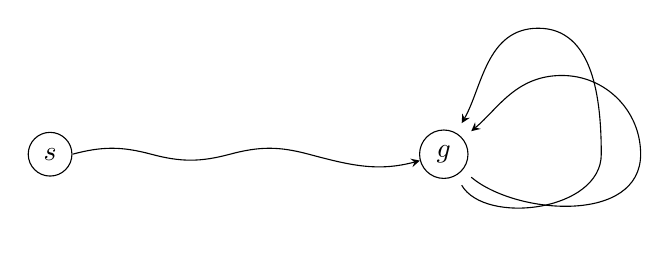
\begin{tikzpicture}
\path node[circle,draw] (s) {$s$} ++ (5,0) node[circle,draw] (g) {$g$};
\draw[-stealth] (s.east) to[out=15,in=165] ++ (1,0)
        to[out=-15,in=-165] ++ (1,0) to[out=15,in=165] ++ (1,0)
        to[out=-15,in=-165](g);
\draw[-stealth,shorten >=4pt,shorten <=4pt] (g) to[out=-40,in=-90] ++ (2.5,0) to[out=90,in=0]
        ++ (-1,1) to[out=180,in=40] (g);
\draw[-stealth,shorten >=4pt,shorten <=4pt] (g) to[out=-60,in=-90] ++ (2,0) to[out=90,in=0]
        ++ (-0.8,1.6) to[out=180,in=60] (g);
\end{tikzpicture}
    \caption{Accepting run of a \gls{BA}}
    \label{Accepting run}
\end{figure}

\begin{figure}[!ht]
    \centering
    \scalebox{0.7}{\input{figures/fig_bmc}}
    \caption{Bounded Model Checking}
    \label{figbmc}
\end{figure}

\begin{eg}
    We illustrate bounded model checking in Figure.~\ref{RunExample}, where we would like to check the temporal property that the letter $a$ occurs sometime in the future and reoccurs infinitely often. Now, this can occur, in a non-looping \emph{stem} part of the run, or in the infinite \emph{loop} of the run (cf.Fig.~\ref{Accepting run}). Notice that the initial state $q_0$ does not accept the letter \emph{a}. In order to know, if there is some state, where \emph{a} is accepted in the future, one needs to look at the next states, apart from the initial state. Using the principle of bounded model checking, we check if \emph{$\neg$ a} is accepted in a \emph{stem} or in \emph{loop} of all the runs possible in the model. The presence of an accepting run, acts as a counterexample to the property being checked. In this case, the sequence of states $q_0,q_2,q_3,q_2,q_3,\ldots$ is a counterexample trace. We can also view this as reaching a state, that accepts the said property.
\end{eg}

In  Chapter.~\ref{chlogics}, we describe how to formally specify the properties in a formal manner using a logical language.
One drawback is that we cannot explicitly represent concurrency in this model, hence we look at more suitable models to represent concurrency in unbounded client server systems via Petri nets, $\nu$-nets (Petri nets with names), and Elementary Object Systems (Petri nets with nesting) in Chapter.~\ref{chmodels}. We revisit this notion of automatically performing bounded model checking, while verifying various models and properties in Sec.~\ref{sec:encodingLTL} and Sec.~\ref{ssec:verif} using a set of specialized tools called SAT/SMT solvers. Given a set of constraints, such as in bounded model checking, SAT/SMT solvers can efficiently check if there exists a \emph{satisfying assignment} of values to those constraints. SAT solvers work with Boolean values. SMT solvers offer various underlying theories such as bit vectors and integer arithmetic~\cite{MouraB08,BarbosaBBKLMMMN22}.



\section{Contributions}
In this thesis, we focus on verification of unbounded client server systems and representing them by various suitable formal models as well as verifying the properties of the systems specified using various logics. In this system, there are unbounded interactions between the single server and unboundedly many clients that are not known apriori. The interactions are restricted to requests by the clients that are responded to, by the server. We have not worked with systems where there are interactions between the clients, nor have we worked with the multiple server multiple client systems. These extensions can be interesting future work.
The major contributions of this work are the following:

\begin{enumerate}

    \item \textbf{Formulated the $2$D-BMC algorithm}. We extend the standard \acrfull{BMC} algorithm to two dimensional bounded model checking, i.e., $2$D-BMC that exploits the two dimensional unboundedness in the Petri nets representing the unbounded client server systems, i.e., unboundedness in the number of clients as well as unbounded concurrency. This is particularly helpful for verifying systems with true concurrency. (See Chapter.~\ref{chproblem})
    \item  \textbf{Verification of a Linear Temporal Logic with integer arithmetic properties on Petri nets using $2$D-BMC:} Built a tool to verify Linear Temporal Logic with integer arithmetic properties on Petri nets. The tool employs SMT solvers to perform the verification queries using an extension of BMC, called the $2$D-BMC algorithm. This tool competes with state of the art \Gls{PetriNet} verification tools and is the first of its kind to use various semantics of Petri nets. (See Chapter.~\ref{chltl})
    \item \textbf{Verification of a variant of  First Order Logic on Petri nets using $2$D-BMC:} Implemented a tool to verify properties of First Order Logic with monodic restriction on Petri nets with identifiers, called $\nu$-nets and which employs SMT solvers to perform the verification queries using $2$D-BMC algorithm. (See Chapter.~\ref{chmfotl})
    \item \textbf{Charted the decidability status of Elementary Object Systems:} The notion of coverability is to ask, given a model and its configuration, is there a second reachable configuration that is smaller than the original configuration. These are important questions in Petri nets and also by extension, in Elementary Object Systems (EOS), which are essentially nets with nesting. In the interactions in the EOSs, imperfect steps are possible, which we call lossiness. Lossiness can occur at various levels of nesting in the EOSs. We charted the decidability status of reachability and coverability problems in EOSs in the case of lossiness at various nesting levels. (See Sec.~\ref{sec:fullLossydecidability})
    \item \textbf{Verification of  reachability of Elementary Object Systems:} The notion of reachability is to ask if a particular configuration can be reached. We implemented an open source tool to verify reachability properties on a class of higher order Petri nets with nesting, called Elementary Object Systems. (See Sec.~\ref{sec:EOSTool})

\end{enumerate}





\begin{comment}

%\subsection*{$\omega$-regular expression}
\begin{dfn}
    An $\omega$-regular expressions is of the form $r_1 s_1^{\omega} +\ldots + r_n s_n^{\omega}$ with standard regular expressions $r_1 , s_1 ,\ldots , r_n ,s_n$.    The semantics of those expressions is defined in a manner analogous to standard regular expressions. For an expression $s$, which defines the language $U \subseteq \Sigma^*$ , the expression $s^\omega$ defines the $\omega$-language $U^\omega$.
\end{dfn}


\begin{eg}
    Consider the following $\omega$-regular expression~\cite{Mukund12}:
    \beq
    (a+b)^*a^\omega + (a+b)^*(ab)^\omega
    \enq

    The corresponding B\"uchi automaton can be drawn as follows:
    \begin{figure}[ht]
        \centering
        \input{figures/1_omegareg}
        \label{regular expression}
        \caption{$\omega$-regular expression}
    \end{figure}

\end{eg}
It may be useful to think in terms of $\omega$-regular expressions, as they can be helpful in characterising the B\"uchi automaton.

\subsubsection{Deterministic and Non deterministic Automata}

\begin{figure}[ht]
    \centering
     \begin{tikzpicture}[shorten >=1pt,node distance=2cm,on grid,auto]
\node[state,initial,accepting] (q_0)   {$s1$};
\node[state] (q_1) [ right=of q_0] {$s2$};
\path[->]
(q_0) edge[above, bend left=15]  node {b} (q_1)
edge [loop above] node {a} ()
(q_1) edge[loop above]  node {b} ()
edge[above, bend left =15] node{a} (q_0)
;
\end{tikzpicture}
    \caption{Deterministic automaton recognizing $L$}
    \label{DeterministicBA}
\end{figure}

Consider the language $L$ over $\{a, b\}$  containing all words that contain infinitely many occurrences of $a$. The deterministic automaton with two states recognizes $L$ with a  B\"uchi condition $\{s1\}$ as in Figure~\ref{DeterministicBA}.

Consider the complement of language $L$ over $\{a, b\}$, $\overline{L}$ set of all infinite words $\alpha$ such that $\alpha$ has only finitely many occurrences of $a$.
The automaton guesses a point in the input beyond which it will see no more $a$'s. There is no deterministic automaton recognizing $\overline{L}$. The automaton in Figure~\ref{NBA} accepts $\overline{L}$.

\begin{figure}[ht]
    \centering
    \begin{tikzpicture}[shorten >=1pt,node distance=2cm,on grid,auto]
\node[state,initial] (q_0)   {$s1$};
\node[state,accepting] (q_1) [ right=of q_0] {$s2$};
\path[->]
(q_0) edge[above]  node {b} (q_1)
        edge [loop above] node {a,b} ()
        (q_1) edge[loop above]  node {b} ();
\end{tikzpicture}
    \caption{Non deterministic automaton recognizing $\overline{L}$}
    \label{NBA}
\end{figure}
\end{comment}

\chapter{Models for Unbounded Concurrency}\label{chmodels}

While formally verifying infinite state systems with concurrency, it is imperative to capture their behaviour in suitable abstract models.
In this chapter, we discuss the various abstractions for modeling concurrent systems that are used in the rest of the thesis.

\section{Petri nets}\label{sec:pn}
Petri nets are a commonly used formalism for modeling the dynamic behaviour of systems~\cite{murata89,petri1962kommunikation}. Here, we recollect the standard notions associated with nets.
\begin{figure}[ht]
    \centering
    	\begin{tikzpicture}[scale=0.45]
	
		
%source transition
 \node[transition,fill=black,minimum height=.4cm,minimum width=.4cm,label=left:{\small $t_{0}$}] (t0) at (-10,0) {};
		
\node[place,label=above:{\small $p_{0}$},draw=red!50,inner
sep=0pt,minimum height=.40cm, minimum width=.5cm] (p0) at (-8,0){$\bullet$} ;	
		
\node[transition,fill=black,minimum height=.4cm,minimum width=.4cm,label=above:{\small $t_{1}$}] (t1) at (-6,0) {};

\node[place,label=above:{\small $p_{1}$},draw=red!50,inner
sep=0pt,minimum height=.40cm, minimum width=.5cm] (p1) at (-4,2){} ;
	
\node[place,label=below:{\small $p_{2}$},draw=red!50,inner
sep=0pt,minimum height=.40cm, minimum width=.5cm] (p2) at (-4,-2){} ;


\node[transition,fill=black,minimum height=.4cm,minimum width=.4cm,label=above:{\small $t_{2}$}] (t2) at (-2,2) {};

\node[transition,fill=black,minimum height=.4cm,minimum width=.4cm,label=above:{\small $t_{3}$}] (t3) at (-2,-2) {};

\node[place,label=above:{\small $p_{3}$},draw=red!50,inner
sep=0pt,minimum height=.40cm, minimum width=.5cm] (p3) at (0,0){} ;

\draw[->] (t0) -- (p0);
\draw[->] (p0) -- (t1);
\draw[->] (t1) -- (p1);
\draw[->] (t1) -- (p2);

\draw[->] (p1) -- (t2);
\draw[->] (p2) -- (t3);

\draw[->] (t2) -- (p3);
\draw[->] (t3) -- (p3);

\draw[->] (p3) node[midway, above]{} (t0);
\end{tikzpicture}
    \caption{A simple Petri net $N_0$ with marking $\langle 1,0,0,0 \rangle$}
    \label{fig:petrinet1000}
\end{figure}

\begin{dfn}\label{def:pn}
    A \emph{PN} is a tuple $N=(P,T,F)$ where $P$ is a finite set of  \emph{places}, $T$ is a finite set of \emph{transitions}, $F : (P \times T) \cup (T \times P)\longrightarrow \mathbb{N}$ is the \emph{flow function}.
    Additionally, if the arcs are allowed to have weights, they are called \emph{weighted} Petri nets. Hence, we also have the weight function $W:F\rightarrow \mathbb{N}_0$, where $\mathbb{N}_0$ is the set of non-negative integers. In Fig.~\ref{fig:petrinet1000}, $P=\{p_0,p_1,p_2,p_3\}$, $T=\{t_0,t_1,t_2,t_3\}$ and $F$ is represented graphically by the directed arcs.
\end{dfn}






\begin{dfn}\label{defn:prepostPN}
    The set $\pre{t}=\{p\in P\mid F(p,t)>0\}$ is called the \emph{set of pre-places} of $t \in T$.
    The set $\post{t} =\{p\in P\mid F(t,p)>0\}$ is called the \emph{set of post-places} of $t \in T$.
\end{dfn}
For instance, in Fig.~\ref{fig:petrinet1000}, $\pre{t_0}=\emptyset$, $\pre{t_1}=\{p_0\}$, $\pre{t_2}=\{p_1\}$, $\pre{t_3}=\{p_2\}$.
And $\post{t_0} =\{p_0\}$, $\post{t_1} =\{p_1,p_2\}$, $\post{t_2} =\post{t_3} =\{p_3\}$.
The flow function $F$ is also described by the pre and post condition functions.

\begin{dfn}
    Given a PN $N=(P,T,F)$, the \emph{pre-condition function} $\prefun_N$ and the \emph{post-condition function} $\postfun_N$ are defined as follows:
    \begin{align*}
        {\prefun}_N : T\rightarrow ( P\rightarrow \mathbb{N})  & \quad\prefun_N(t)(p)=F(p,t)  \\\quad
        {\postfun}_N : T\rightarrow ( P\rightarrow \mathbb{N}) & \quad\postfun_N(t)(p)=F(t,p)
    \end{align*}
\end{dfn}


The states of the PN are the distributions of tokens in the places, described by \emph{markings}.

\begin{dfn}
    A \emph{marking} $M$ of a PN $N=(P,T,F)$ is a function $M : P \rightarrow \mathbb{N}_0$, where $\mathbb{N}_0$ is the set of non-negative integers. A \emph{marked PN} is a pair $PN=(N,M_0)$ where $N$ is a PN and $M_0$ is a marking, called \emph{initial marking}.
\end{dfn}

In Fig.~\ref{fig:petrinet1000} the marking $\langle 1,0,0,0 \rangle$, denotes the distribution of tokens in the places.

\begin{dfn}[Enabledness Rule] A transition $t$ is enabled at marking $M$
    when $\forall p\in P, M(p)\geq \prefun_N (t,p)$.
\end{dfn}
The \emph{enabledness rule} is a prerequisite for firing a transition $t$. On the firing of $t$, the successor of the current marking is obtained according to its pre and post conditions, i.e., by removing $F(p,t)$ tokens from each $p \in \pre{t}$ and adding $F(t,p')$ tokens to each $p' \in \post{t}$, leaving tokens in the remaining places as they are.

\begin{dfn}[Firing Rule]
    Given a marking $M$ in a Petri net, on firing an enabled transition $t$, we get the successor marking $M'$, denoted by $M \xrightarrow{t} M'$, such that:
    \begin{align*}
        %\forall p \in \pre{t}, p' \in \post{t}: M(p) \geq Pre(p,t) \land 
        \forall p\in P:
        M'(p) = M(p) - F(p,t) + F(t,p)
    \end{align*}
\end{dfn}



If there are several enabled transitions at a given marking, exactly one of them is non-deterministically chosen to be fired in the step.


\begin{figure}[ht]
    \centering
    \input{figures/fig_pn1}
    \caption{A simple Petri net $N_0$ with marking $\langle 0,1,1,0 \rangle$}
    \label{fig:petrinet0110}
\end{figure}

Given the marking in Fig.~\ref{fig:petrinet1000} and on firing transition $t_1$, the marking in Fig.~\ref{fig:petrinet0110} is obtained.



\begin{dfn}
    The set of markings \emph{reachable} from marking $M$ in a given net $N$, denoted by $reach_N(M)$, is the smallest set of markings such that:
    \begin{itemize}
        \item $M \in reach_N(M)$ and
        \item If $M'\xrightarrow{t}M''$ for some $t\in T$ and $M' \in reach_N(M)$, then $M'' \in reach_N(M)$.
    \end{itemize}
    The \emph{reachability graph} of a PN $N$ is the directed graph $(\N,E)$ where $\N$ is the set of markings of $N$, $E\subseteq \N\times\N$, and $(M,M')\in E$ iff there is some $t\in T$ such that $M\xrightarrow{t}M'$. The set of reachable markings of a marked PN $(N,M_0)$, is $reach_N(M_0)$.
\end{dfn}

\begin{dfn}[Unbounded Petri Net]\label{dfn:unboundedPN}
    An unbounded Petri Net is a Petri Net $N=(P,T,F)$ where $P$ is a finite set of  \emph{places}, $T$ is a finite set of \emph{transitions}, $F : (P \times T) \cup (T \times P)\longrightarrow \mathbb{N}$ is the \emph{flow function} where the $reach_N(M_0)$ is infinite.
\end{dfn}
Alternatively, it means that there is no finite integer \(k\) such that every place \(p\in P\) has fewer than \(k\) tokens (\(M(p)\le k\)) for all reachable markings \(M\).

\begin{dfn}[Conservative Petri net]
    A PN $N=(P,T,F)$ is \emph{conservative} iff
    \begin{align*}
        \forall p \in P \,  \forall t \in T : F(p,t) = F(t,p)
    \end{align*}
\end{dfn}


\begin{figure}[ht]
    \centering
    \begin{tikzpicture}[scale=0.45]


\node[place,label=left:{\small $p_{0}$},draw=red!50,inner
sep=0pt,minimum height=.40cm, minimum width=.5cm] (p0) at (-4,2){$\bullet$} ;	

\node (i0) at (-1.5,1.5) {$1$};
\node (i1) at (-1.5,-1.5) {$2$};
		
\node[place,label=left:{\small $p_{1}$},draw=red!50,inner
sep=0pt,minimum height=.40cm, minimum width=.5cm] (p1) at (-4,-2){$\bullet\bullet$} ;

\node[transition,fill=black,minimum height=.4cm,minimum width=.4cm,label=above:{\small $t_{0}$}] (t0) at (0,0) {};

\node[place,label=right:{\small $p_{2}$},draw=red!50,inner
sep=0pt,minimum height=.40cm, minimum width=.5cm] (p2) at (4,2){$\bullet\bullet$} ;	

\node (i2) at (1.5,1.5) {$2$};
\node (i3) at (1.5,-1.5) {$1$};
		
\node[place,label=right:{\small $p_{3}$},draw=red!50,inner
sep=0pt,minimum height=.40cm, minimum width=.5cm] (p3) at (4,-2){$\bullet$} ;

		
\draw[->] (p0) -- (t0);
\draw[->] (p1) -- (t0);
\draw[->] (t0) -- (p2);
\draw[->] (t0) -- (p3);
\end{tikzpicture}
    \caption{A conservative Petri net $N_1$}
    \label{fig:petrinet3}
\end{figure}

A Petri net $N$ is said to be \emph{conservative}, if all transitions fire token-preservingly, i.e., all transitions add exactly as many tokens to their post-places as they subtract from their pre-places. This is illustrated in Fig.~\ref{fig:petrinet3}.

Markings are naturally ordered by the coverability relation $\leq$, defined as follows.

\begin{dfn}
    Given two markings $M_1$ and $M_2$, we say that a marking $M_2$ covers $M_1$, denoted by $M_1 \leq M_2$, iff $\forall p \in P, M_1(p) \leq M_2(p)$.
\end{dfn}

In Petri net $N_1$ from Fig.~\ref{fig:petrinet1000} suppose the marking $M_0 =\langle 0,0,0,0 \rangle$ and on firing $t_0$ we obtain $M_1=\langle 1,0,0,0 \rangle$, we say that $M_1$ covers $M_0$.

The \emph{reachability problem} is as follows: given a marked PN $(N,M_0)$ and a marking $M$, whether $M\in reach_N(M_0)$. For instance, in Fig.~\ref{fig:petrinet3}, given the initial marking, $M_0$ is $\langle 1,2,2,1 \rangle$. We know that the marking $M_1=\langle 0,0,4,2 \rangle = reach_{N_1}(M_1)$. Hence, $M_1\in reach_{N_1}(M_1)$.

It is known that the reachability problem for PN is \emph{decidable} but in non-primitive recursive time~\cite{CzerwinskiLLLM21}. The \emph{coverability problem} is as follows: given a marked PN $(N,M_0)$ and a marking $M$, whether there is a reachable marking $M'\in reach_N(M_0)$ such that $M'\leq M$. It is known that also the coverability problem is decidable and in EXPSPACE~\cite{Rackoff78}. Another problem on PN is \emph{deadlock-freeness}.

\begin{dfn}[Dead Marking]
    A marking $M$ for net $N$ is \emph{dead} if transition $t$ is not enabled at $M$ for all $t\in T$. The marked PN $(N,M_0)$ is \emph{deadlock-free}, if there is no dead marking in $reach_N(M_0)$.
\end{dfn}

For instance, in Fig.~\ref{fig:petrinet1000}, if the net is modified such that the transition $t_0$ is not present, it would result in a deadlock after obtaining the marking $\langle 0,0,0,2\rangle$.
The \emph{deadlock-freeness} problem is as follows: given a marked PN $N$, whether $N$ is deadlock-free.
It is well-known that deadlock-freeness and reachability are recursively equivalent and, thus, deadlock-freeness is decidable but in non-primitive recursive time complexity~\cite{Hack74,ChengEP95}.

\subsection{Petri net Semantics}\label{ssec:pnsemantics}

In this section, we look at the formal sematics of Petri nets, in particular the interleaving and concurrent semantics. The key difference in the two approaches, is in the firing condition. We recall the firing rule:

Given an enabled transition $t$ at marking $M$, on firing $t$, we get the successor marking $M'$, denoted by $M \xrightarrow{t} M'$, such that:
\begin{align*}
    \forall p\in P:
    M'(p) = M(p) - F(p,t) + F(t,p)
\end{align*}


In interleaving semantics, there is atmost one transition that is fired in an instance or step of the occurrence sequence. Given an initial marking $M_0=\tup{0,0,0,0}$, on firing $t_0$ twice and $t_1$ once, we obtain this sequence
$\tup{0,0,0,0} \xrun{t_0}\tup{1,0,0,0}\xrun{t_0}\tup{ 2,0,0,0} \xrun{t_1}\tup{0,1,1,0} $ as depicted in Fig.~\ref{fig:petrinet0110}.




\begin{recallfigure}[!ht]{fig:petrinet0110}
    \centering
    \input{figures/fig_pn1}
    \caption{Recall the simple Petri net $N_0$ with marking $\langle 0,1,1,0 \rangle$}
\end{recallfigure}


\begin{figure}[ht]
    \centering
    \input{figures/fig_pn2}
    \caption{Petri net $N_0$  with marking $\langle 0,0,0,2 \rangle$}
    \label{fig:petrinet0002}
\end{figure}

Now, both transitions $t_2$ and $t_3$ are enabled. In interleaving semantics, one may fire either of the two transitions, one after the other.
However, in concurrent semantics, the following sequence is also additionally possible in a single step, resulting in Fig.~\ref{fig:petrinet0002}.

$\langle 0,1,1,0\rangle \xrun{t_2,t_3}\langle 0,0,0,2\rangle $

\begin{dfn}[Concurrent Firing Rule]\label{defn:concurfirerule}

    Given a Petri net $N$ and a marking $M$ having a set of enabled transitions $\tau \in T$, we obtain the successor marking $M'$ on concurrent firing of a subset of transitions $\tau'\subseteq \tau$ using the following rule:

    %Given a set of enabled transitions $\tau \in T$ at marking $M$, on firing $\tau$, we get the successor marking $M'$, denoted by $M \xrightarrow{\tau} M'$, such that:
    \begin{align*}
        %\forall p\in P:M'(p) = M(p) - F(p,t) + F(t,p)
        \forall p\in \pre{\tau '}:
        M'(p) = M(p) -\sum_{t\in \tau'} F(p,t) + \sum_{t \in \tau'}F(t,p)
        \text{ if } \sum_{t\in \tau'} F(p,t) - M(p) \geq 0.
    \end{align*}
\end{dfn}

The condition $\sum_{t\in \tau'} F(p,t) - M(p) \geq 0$ takes care of the sufficiency of tokens at each of the pre-places of the transitions in $\tau'$ such that the transitions can be fired. This is a particularly elegant rule in the context of representing concurrent firing of transitions in a Petri net in a SMT solver. This automatically addresses scenarios where the firing of one transition might disable another, the resultant set of transitions that are subsequently fired are all valid transitions that are enabled and whose concurrent firing is allowed by the Petri net semantics.


\begin{figure}[ht]
    \centering
    \begin{tikzpicture}[scale=0.45]


\node[place,label=left:{\small $p_{0}$},draw=red!50,inner
sep=0pt,minimum height=.40cm, minimum width=.5cm] (p0) at (-4,2){$\bullet$} ;	

\node (w0) at (-2,2.5) {$w_0$};
\node (w1) at (-2,-1.5) {$w_1$};
		
\node[place,label=left:{\small $p_{1}$},draw=red!50,minimum height=.40cm, minimum width=.5cm] (p1) at (-4,-2){$\bullet\bullet$} ;

\node[transition,fill=black,minimum height=.4cm,minimum width=.4cm,label=above:{\small $t_{0}$}] (t0) at (0,2) {};


\node[transition,fill=black,minimum height=.4cm,minimum width=.4cm,label=above:{\small $t_{1}$}] (t1) at (0,-2) {};

\node (w1) at (-2,-5) {$w_1$};

\node[transition,fill=black,minimum height=.4cm,minimum width=.4cm,label=above:{\small $t_{2}$}] (t2) at (0,-6) {};

\node[place,label=right:{\small $p_{2}$},draw=red!50,minimum height=.40cm, minimum width=.5cm] (p2) at (4,-2){} ;

\node (w1) at (2.5,-1.5) {$w_2$};

\node[place,label=right:{\small $p_{3}$},draw=red!50,minimum height=.40cm, minimum width=.5cm] (p3) at (4,-6){} ;		

\node (w1) at (2.5,-5.5) {$w_3$};

		
\draw[->] (p0) -- (t0);
\draw[->] (p1) -- (t0);
\draw[->] (p1) -- (t1);
\draw[->] (t1) -- (p2);
\draw[->] (p1) -- (t2);
\draw[->] (t2) -- (p3);
\end{tikzpicture}
    \caption{Concurrent Firing of Petri net $N_1$}
    \label{fig:pnconcur}
\end{figure}

In Fig.~\ref{fig:pnconcur}, $P=\{p_0,p_1,p_2,p_3\}$ and $T=\{t_0,t_1,t_2\}$. Given an initial marking $M_0=\langle 1,2,0,0\rangle$, the set of enabled transitions w.r.t $M_0$, is $\tau=\{t_0,t_1,t_2\}$. Suppose $\tau'=\{t_1,t_2\}$, then $\pre{\tau '}=\{p_1\}$ and the step $\langle 1,2,0,0\rangle \xrun{t_1 \& t_2}\langle 0,0,1,1\rangle $ is allowed by the concurrent firing rule stated above. However, suppose $M_1=\langle 1,1,0,0\rangle$, $\tau'=\{t_1,t_2\}$  and $\pre{\tau '}=\{p_1\}$, then the step $\langle 1,1,0,0\rangle \xrun{t_1 \& t_2} $ is not allowed by the same rule.

\emph{Remark:} Given a PN where transitions $t_1, t_2, \cdots t_n$ are enabled and there are sufficient tokens in the pre places of $t_1, t_2, \cdots t_n$ such that the transitions may be fired, in the context of true concurrent semantics, we wish to fire maximal number of transitions, wherever possible. Consequently, this means that if there are intermediate markings, which are reachable by an interleaved firing of a subset of the transitions $t_1, t_2, \cdots t_n$, then those markings become unreachable when executing in a truly concurrent manner.

\section{Petri net Representation for an SMT Solver}\label{sec:pnrepresentation}

The bigger picture is to verify properties of the Petri net using an SMT solver~\cite{HandbookSMTBarrettT18}. Satisfiability of formulas with respect to a particular theory such as arrays, integer arithmetic, bit vectors is called as Satisfiability Modulo Thoery. The tools employing the decision procedures and programs to solve these satisfiability constraints are known as SMT solvers. Well known SMT solvers include Z3, CVC4~\cite{MouraB08,BarrettCDHJKRT11}. In this section, we discuss the representation of nets such that they can be added as constraints in an SMT solver, namely Z3. The Petri net representation with interleaving semantics and the true concurrent semantics differ. While verifying infinite state systems,~\cite{AbdullaJ01} employed backwards reachability for proving safety properties, and in case of concurrent programs, ~\cite{AbdullaJRS06} proved liveness and termination via backwards reachability. In the unbounded Petri net setting,~\cite{AbdullaIN00} is the last known work where unfoldings (in the sense of Ken McMillan~\cite{KenUnfolding92}) are discussed from a verification point of view. In state of the art Petri net verification tools, interleaving semantics is adopted~\cite{AmatDH22}. We take an alternate perspective of this and unfold unbounded Petri nets with true concurrency using the help of SMT solvers. In this thesis, by unfolding, we refer to the process of obtaining the subsequent configurations from the initial marking of the net. This is not to be confused with the notion of unfolding described by Ken McMillan in his seminal work on partial orders~\cite{KenUnfolding92}.

We outline the variables and data structures that are necessary to describe the true concurrent semantics. We have a finite set of transitions, $t_0,\ldots,t_m$ described in the net, their names are in the list $tNames$. We have a finite set of places, $p_0,\ldots,p_l$ their names are in the list $pNames$. Arcs can be of either of two types: where the source is a transition and the target is a place or the source is a place and the target is a transition. The net formalism does not allow arcs between places and between transitions themselves. If they occur, the net description is erroneous, and we cannot move ahead with the unfolding.

We use the vector $iWTk$ to store the expressions with respect to $k$, to compute the incident weights of transitions. We use the vector $WTk$ to store the expressions with respect to $k$, to denote the change in weights for places.
We use two-dimensional matrices $Wt[m][l]$ and $iWt[m][l]$ to denote the net change in weights and the incidence weights (outgoing from places). The expressions for the same are stored in $WTVars$ and $iWTVars$ respectively.

We construct the two-dimensional weight matrix $Wt[row][col]$ of size $m \times l$ which contains the net weight of the arcs. Initially, all the matrix entries are initialized to zero.

For an arc from place $p_i$ to transition $t_j$ with the weight $w$, we have the matrix entry $Wt[i][j] = Wt[i][j] - w$.
For an arc from transition $t_j$ to place $p_i$ with the weight $w$, we have the matrix entry $Wt[i][j] = Wt[i][j]  + w$. Now, if there are incoming and outgoing arcs of the same weights, then the net weight $Wt[i][j]=0$. Notice that, by looking only at the Wt matrix, we may not distinguish between the case where there are no arcs to and from an element of the net. Hence, it is necessary to have a separate data structure for the same. We have a two-dimensional matrix $iWt[row][col]$ of size $m \times l$ which contains the incident weights to the transitions.
For an arc from place $p_i$ to transition $t_j$ with the weight $w$, we have the matrix entry $iWt[i][j] =Wt[i][j] - w$. The marking of the net consists of the set tokens at each place and represents the state of the net at any instance.
The initial marking of the net can be obtained from the net description and contains the number of tokens in each of the places $p_0,\ldots,p_l$ in the net. The subsequent markings may be constructed from the matrix $Wt$ and using the transition function of the net. The transition function $TF$ describes the behaviour of the net. The initial marking of the net is stored in $initial$. We introduce a method $printTFTruthTable$ that can aid to visualise the transition function $TF$ which is an expression describing the function. Most utility methods and the $2-DBMC$ algorithm are similar to that of the interleaving semantics. For experimentation, we have three different versions for constructing the Transition Function which are equivalent to each other (as verified by truth tables, experiments with $352$ properties) and are a simplification of the expression using $\land \land $, $||$ instead of $\implies$ and so on. Experiments suggest that one version is slightly faster than the others. The variable $T[ti]$ denotes the $i$th transition being fired. Hence the expression $!T[ti]$ denotes that the $i$-th transition is not fired. For every pair of transitions and places, if there are no outgoing arc from the transition $t_i$ then the expression $preCond$ containing the precondition for firing of transitions is constructed as follows:
\vspace{-20pt}
\begingroup
\allowdisplaybreaks
\begin{align}
    if (emptyOutTi)     & \{                                                  \\
    preCond             & = (tmp == iWt[pi][ti] \lor tmp == 0)                \\
                        & \land ((T[ti] \land  tmp == iWt[pi][ti])            \\
                        & \lor (!T[ti] \land tmp == 0))                       \\
    cumulativeIncidentW & = tmp                                               \\
    emptyOutTi          & = !emptyOutTi\}                                     \\
    else\{              &                                                     \\
    preCond             & = preCond \land  (tmp == iWt[pi][ti] \lor tmp == 0) \\
                        & \land ((T[ti]\land tmp == iWt[pi][ti])              \\
                        & \lor  (!T[ti] \land tmp == 0))                      \\
    cumulativeIncidentW & = cumulativeIncidentW + tmp\}
\end{align}
\endgroup
The sum of incident weights at a transition $t_i$ is stored in $cumulativeIncidentW$ as an expression of the $iWt[pi][ti]$ if there is an arc from the transition $t_i$ to place $p_i$ or it is zero. If the transition is not fired, then there are no weights to be considered.

If the expression is non-empty, the previously constructed $preCond$ are \textbf{anded} with the newly constructed expression and the cumulative incident weights are updated in the same manner.

The post condition is constructed if the weight $Wt[pi][ti]!=0$.
\begin{align*}
    postCond          & = ((tmp == Wt[pi][ti]) \lor (tmp == 0) \\
                      & \land((T[ti] \land  tmp == Wt[pi][ti]) \\
                      & \lor (!T[ti]\land  tmp == 0))          \\
    cumulativeWChange & = tmp                                  \\
    emptyChangePi     & = !emptyChangePi
\end{align*}
Based on the above expressions, we construct the transition function $TF$
\begin{verbatim}
    if (emptyTF){
            if (!emptyOutTi){
                TF = preCond & (Px[pi] + cumulativeIncidentW >= 0) 
                emptyTF = false}
            if (!emptyChangePi){                    
                if (!emptyOutTi)
                    TF = TF & postCond 
                    &(Py[pi] == Px[pi] + cumulativeWChange)
                else
                    TF = postCond &(Py[pi] == Px[pi]
                     + cumulativeWChange)
                emptyTF = false
                }
        }
        else{
            if (!emptyOutTi)
                TF = TF &preCond 
                &((Px[pi] + cumulativeIncidentW) >= 0)
            if (!emptyChangePi)
                TF = TF &postCond
                 &(Py[pi] == (Px[pi] + cumulativeWChange))
        }
\end{verbatim}
The transition function is a conjunction of the preconditions, postconditions and the change in the markings. In case of interleaving semantics, there is an additional conjunction to the transition function, a disjunction of each transition $t_i$, to ensure that exactly one transition is fired in a step.

\subsection{$\nu$-nets}\label{ssec:nunetsmodel}
In the rest of this thesis, we consider the specific setting of single server multiple client systems, with distinguishable clients. These distinguishable clients are represented using distinguishable tokens of the Petri net, i.e., tokens appended with identifiers~\cite{VelardoF07}. There are an unbounded number of clients and a fresh client identifier is issued whenever a new client enters the system. When clients exit, the identifiers need to be purged. While the case study is discussed in detail in Chapter.~\ref{chproblem}, here, we outline the requirements for the formal model and arrive at a suitable representation.

As seen in the Sec.~\ref{sec:pn}, Petri nets are suitable to model the \emph{concurrent} behaviour of the clients and are also suitable to capture an unbounded number of clients. The places correspond to the local states of the client and server. We have a disjoint set of server places and client places. The combined interactions of the server and client processes are represented by transitions. The tokens correspond to the processes (server process, client process). Unbounded Petri nets with indistinguishable tokens are not sufficient to differentiate between processes (server process, client process). Hence we look for another model.
At first glance, a candidate model is the colored Petri net (CPN)~\cite{JensenCPN07} which satisfies the above requirements. CPNs allow arbitrary expressions over user-defined syntax labelling the arcs, and the underlying modeling language (such as CPN Modeling Language in  CPN Tools~\cite{JensenKW07}) is highly expressive. However, we do not prefer the CPN, for the following engineering reasons.

First, there is a dearth of tools to automatically \emph{unfold} unbounded colored Petri nets. Recall that the big picture is the automatic verification of unbounded client-server systems. Alternatively, suppose we represent the formal model as a CPN such as using CPN Tools, there are no existing tools that can automatically \emph{unfold} an \emph{unbounded} CPN created using CPN Tools. Existing tools can only unfold \emph{bounded} CPNs~\cite{Dal-Zilio20,BilgramJPST22}. The second candidate model is a type of $\nu$-net~\cite{VelardoF08}, which is a CPN defined over a system of component nets, which use a labelling function $\lambda$, to handle synchronization between multiple component nets of a larger net system.

We restrict the $\nu$-nets to a single component, providing a simplified
definition while doing away with the labelling function used in $\nu$-nets.
% For our case study, this representation is sufficient to model the single server multiple client behaviour by composing the client and server behaviour in a compact manner and restricting ourselves to a single component. 
The client behaviour can be represented as a state machine. Similarly the server behaviour can also be represented as a state machine.
In this representation, we describe the behaviour of the single server multiple client system as a single component.

We begin with some definitions that are necessary for describing the restricted $\nu$-net. Given an arbitrary set $A$, we denote by $\mathcal{MS}(A)$, the set of finite multisets of A, given by the set of mappings $m:~A\to \mathbb{N}$. We denote by $S(m)$ the support of m, defined as follows:
$S(m)=\{a\in A \mid m(a)>0\}$. Distinguishable tokens (identifiers) are taken from an arbitrary infinite set \emph{Id}. To handle this, we add matching variables labeling the arcs, taken from a set $Var$. To handle the movement of tokens inside the $\nu$-net, we employ a finite set of variables, $Var$ using which we label the arcs of the net. There is a special variable $\nu\in Var$, which introduces tokens into the place, which is described later.

\begin{figure}[ht]
    \begin{center}
        \scalebox{0.8}{\input{figures/2_fig_aps_vnet_v2}}
        \caption{A restricted $\nu$-net modeling an unbounded client-server system}
        \label{fig:APS}
    \end{center}
\end{figure}

\begin{dfn}\label{defn:nunet}
    A $\nu$-net is a coloured Petri net $N=(P,T,F)$, where
    \begin{itemize}
        \item $P$ and $T$ are finite disjoint sets of places and transitions, respectively,
        \item $F$: $(P \times T) \cup (T \times P) \to \mathcal{MS(\text{Var})}$ defines the
              set of arcs of the net, satisfying $\nu \not \in pre(t)$ for every $t
                  \in T$.
    \end{itemize}


    For a transition $t$ of the net, we define, $post(t)=\bigcup_{p\in P} S(F(t,p))$,
    $pre(t)=\bigcup_{p\in P} S(F(p,t))$
    and $Var(t)= pre(t) \bigcup post(t)$.

\end{dfn}

For instance, in Fig.~\ref{fig:APS}, $Var=\{\nu,s,c\}$, $T=$ $\{t_{acc}$, $t_{rej}$, $t_{s\_exit}$, $t_{u\_exit}$, $t_{acc\_sink}$, $t_{rej\_sink}\}$ and $P=\{$ $p_{PR}$, $p_{SR}$, $p_{OP}$, $p_{PU}$, $p_{ES}$, $p_{EU}\}$. $pre(t_{acc})=\{s,c\}$ and $post(t_{acc})=\{s,c\}$, hence $Var(t_{acc})=\{s,c\}$.


\begin{dfn}[Marking]
    A marking  of a restricted $\nu$-net $N=(P,T,F)$ is a function $M:P\to(\mathcal{MS}(Id))$.
\end{dfn}
In Fig.~\ref{fig:APS}, the initial marking $M_0=\langle \{0\}, \{1,2\}, \emptyset, \emptyset, \emptyset, \emptyset \rangle$.

\begin{dfn}[Mode]\label{defn:modenunet}
    We denote by $S(M)$ the set of identifiers in $M$. i.e., $S(M)=\bigcup_{p\in P}S(M(p))$. A mode of a transition $t$ is a mapping $\sigma:Var(t)\to Id$, instantiating every variable in the adjacent arcs of $t$ to some identifier. %Transitions are fired with respect to some mode, that establishes which tokens are taken from preconditions.
\end{dfn}


Let $N$ be a restricted $\nu$-net and $M$ a marking of $N$ according to Defn.~\ref{defn:nunet}.

\begin{dfn}[Enabling Rule]
    We say that $M$ \textbf{enables} the transition $t$ with mode $\sigma$ whenever:

    \begin{itemize}
        \item If $\nu \in Var(t)$ then $\sigma(\nu)\not \in S(M)$ and
        \item $\sigma(F(p,t))\subseteq M(p)$ for all $p \in P$.
    \end{itemize}
\end{dfn}

Notice that if $\sigma(\nu)\not \in S(M)$ for the enabling of transition, that causes the creation of fresh (equal) identifiers in all the places reached by arcs labelled by the special variable $\nu \in Var$ that appears only in post-condition arcs.

\begin{dfn}[Firing Rule]\label{nufire}
    The reached marking of net $N$ after firing of $t$ with mode $\sigma$
    is denoted by $M \xrightarrow{t(\sigma)}M'$, where
    $\forall p \in P: M'(p)=M(p) - \sigma(F(p,t)) + \sigma(F(t,p))$.
\end{dfn}

In Fig.~\ref{fig:APS}, given initial marking $M=\langle \{0\}, \{1,2\}, \emptyset, \emptyset, \emptyset, \emptyset \rangle$ and $M \xrightarrow{t_{acc}} M'$, $M'=\langle \{0\}, \{2\}, \{1\}, \emptyset, \emptyset, \emptyset \rangle$, i.e., the token $\{1\}$ has moved to the place $P_{OP}$. The mode is represented in the figure.

In Fig.~\ref{fig:APS}, the transitions $t_{acc}$, $t_{rej}$, $t_{s\_exit}$, $t_{u\_exit}$, $t_{acc\_sink}$, $t_{rej\_sink}$, represent the accept, reject, exit successfully, exit unsuccessfully and the two sink transitions respectively. A transition is \textbf{identifier-preserving} if $post(t)\setminus \{\nu\}\subseteq pre(t)$. Here, all of them are \emph{identifier-preserving} transitions, which ensures that the system with identified clients is represented correctly modeled. The firing of transition $t_{src}$ acts as the source. The arc labelled $\nu$ ensures that a new client identifier is generated in place $p_{PR}$. The place $p_{PR}$ contains a set of clients requesting for parking.
In the unsuccessful scenario, the transition $t_{rej}$ is fired when the server rejects the request, which brings the vehicle to \emph{parking\_unavailable} state represented by place $p_{PU}$. On firing of transition $t_{u\_exit}$, the vehicle goes to \emph{exited\_unsuccessfully} state represented by place $p_{EU}$.
The firing of transition $t_{rej\_sink}$ is the sink transition for the rejected parking requests. This ensures that the rejected vehicle identifier exits the system and is never reused. If the client arrives after it has exited, it is always issued a fresh identifier.
Notice that there are arcs labelled $s$ to indicate the server which
has identifier $0$, which is necessary for the acceptance or rejection
of a parking request. The token with identifier $0$ is permanently present in each marking
exactly at server place $p_{SR}$. The $\nu$ arc ensures that new
identifiers are generated, essentially giving an unbounded number of
agents in the $\nu$-net. The arcs labelled $c$ carry the client
identifiers from one client place to another. The net behaves as a
standard $\nu$-net component with autonomous transitions as described
in~\cite{VelardoF08}. We explored simple Petri nets, with identifiable tokens. Next, we shall explore an extension of Petri nets, suitable for modeling real world software systems.

\subsection{Elementary object Systems}

In~\cite{valk87,Valk03}, they introduce the nets-within-nets paradigm, wherein, the tokens of the Petri net can be nets themselves. They are used to model the dynamic nature of token behaviour. This is synonymous with the object-oriented modeling approach introduced by Booch~\cite{Booch04}, which most software systems, including client-server systems follow.

In nets-within-nets, one can restrict the nesting of nets, to a nesting depth of two, to obtain Elementary Object Systems (EOSs). Here, the level $0$ net is called the system net and the (nested) level $1$ net is called the object net. In our running example, of the single server multiple clients, we represent server behaviour by the system net and the client behaviour by the object nets that are nested within the system net. In EOSs, we have events, that enable firing of transitions in the system net or object net or at both levels, i.e., system autonomous, object autonomous and synchronized events. Their formal definition is given below:

\begin{dfn}[\textbf{EOS}]\label{def:bussy14_eos}
    An \emph{EOS} $\os$ is a tuple $\os=\tup{\hat{N},\N,d,\Theta}$ where:
    \begin{compactenum}
        \item $\hat{N}=\tup{\hat{P},\hat{T},\hat{F}}$ is a PN called \emph{system net}; $\hat{T}$ contains a special set $ID_{\hat{P}}=\{id_p\mid p\in \hat{P}\}\subseteq \hat{T}$ of \emph{idle transitions} such that, for each distinct $p,q\in \hat{P}$, we have $\hat{F}(p,id_p)=\hat{F}(id_p,p)=1$ and $\hat{F}(q,id_p)=\hat{F}(id_p,q)=0$.
        \item $\N$ is a finite set of PNs, called \emph{object PNs}, such that $\blacksquare\in\N$ and if $(P_1,T_1,F_1), (P_2,T_2,F_2)\in\N \cup \hat{N}$,\footnote{This way, the system net and the object nets are pairwise distinct.} then $P_1\cap P_2=\emptyset$ and $T_1 \cap T_2 = \emptyset$.
        \item $d:\hat{P}\rightarrow \N$ is called the \emph{typing function}.
        \item $\Theta$ is a finite \emph{set of events} where each \emph{event} is a pair $(\hat{\tau},\theta)$, where $\hat{\tau}\in \hat{T}$ and  $\theta:\N \rightarrow \bigcup_{(P,T,F)\in\N} T^\oplus$,
        such that $\theta((P,T,F))\in T^\oplus$ for each $(P,T,F)\in\N$ and, if $\hat{\tau}=id_p$, then $\theta(d(p)) \neq \emptyset$.
    \end{compactenum}
\end{dfn}


\begin{dfn}[Nested Markings]
    Let $\os=\tup{\hat{N},\N,d,\Theta}$ be an EOS. The set of \emph{nested tokens} $\nestTok(\os)$ of $\os$ is the set $\bigcup_{(P,T,F)\in\N} (d^{-1}{(P,T,F)}\times P^{\oplus})$. The set of \emph{nested markings} $\M(\E)$ of $\os$ is $\nestTok(\os)^{\oplus}$.
    Given $\lambda,\rho\in \M(\E)$, we say that $\lambda$ is a \emph{sub-marking} of $\mu$ if $\lambda \sqleq \mu$.
\end{dfn}
Note that $\lambda$ is a sub-marking of $\mu$ iff there is some nested marking $\mu'$ such that $\mu=\lambda+\mu'$. EOSs inherit the graphical representation of PNs with the provision that we represent nested tokens via a dashed line from the system net place to an instance of the object net where the internal marking is represented in the standard PN way. However, if the nested token is $\tup{p,\varepsilon}$ for a system net place $p$ of type $\blacksquare$, we represent it with a black-token $\blacksquare$ on $p$. If a place $p$ hosts $n>2$ black-tokens, then we represent them by writing $n$ on $p$. Each event $\tup{\hat{\tau},\theta}$ is depicted by labeling $\hat{\tau}$ by $\tup{\theta}$ (possibly omitting double curly brackets). If there are several events involving $\hat{\tau}$, then $\hat{\tau}$ has several labels.


\begin{example}\label{ex:cardeos}
    Fig.~\ref{fig:cardpn} depicts the Petri net which
    \begin{inparaenum}[\itshape (1)]
        \item counts the parity of the $a$'s and $b$'s in the input word (firing sequence)
        \item on seeing an $a$, the parity of the alphabet changes and the token moves to the place with $a_O$
        \item on seeing an $b$, the parity of the alphabet changes and the token moves to the place with $b_O$.
    \end{inparaenum}
    The marking $M_0=\tup{1,0,0,0}$ depicts the empty word, with exactly a token in place $a_E b_E$. For instance, given the firing sequences $\sigma=abba$, $M_0 \xrun{\sigma} M_0$.
    Fig.~\ref{fig:cardeos} depicts the equivalent EOS which counts the parity of the $a$'s and $b$'s in the input word.
\end{example}

\begin{figure}[ht]
    \centering
   % \resizebox{.79\columnwidth}{!}{
    \begin{tikzpicture}[scale=0.45]
                \tikzset{
    %Define standard arrow tip
    >=stealth',
    %Define style for boxes
    punkt/.style={
        rectangle,
        rounded corners,
        draw=black, very thick,
        text width=8.5em,
        minimum height=2em,
        text centered},
    % Define arrow style
    pil/.style={
        ->,
        thick,
        shorten <=2pt,
        shorten >=2pt,}
}
\tikzstyle{aldecision} = [diamond, draw, fill=blue!20,
text width=4.5em, text badly centered, node distance=2.5cm, inner sep=0pt]
\tikzstyle{alblock} = [rectangle, draw, fill=blue!20,
text width=5em, text centered, rounded corners, minimum height=4em]
\tikzstyle{line} = [draw, very thick, color=black!50, -latex']
\tikzstyle{allibrary} = [draw, ellipse,fill=red!20, node distance=2.5cm,
minimum height=2em]

\node[place,label=above:{\small $a_E b_E$},draw=red!50,inner
sep=0pt,minimum height=.40cm, minimum width=.5cm, tokens=1] (aEbE) at (-4,0){$\bullet$} ;

\node[transition,fill=black,minimum height=.4cm,minimum width=.4cm,label=above:{\tiny{b}}] (b0) at (0,1) {};

\node[transition,fill=black,minimum height=.4cm,minimum width=.4cm,label=above:\tiny{{b}}] (b1) at (0,-1) {};

\node[place,label=above:{\small $a_E b_O$},draw=red!50,inner
sep=0pt,minimum height=.40cm, minimum width=.5cm] (aEbO) at (4,0){} ;




%Row 2

\node[transition,fill=black,minimum height=.4cm,minimum width=.4cm,label=above:{\tiny{a}}] (a0) at (-5,-3) {};

\node[transition,fill=black,minimum height=.4cm,minimum width=.4cm,label=above:{\tiny{a}}] (a1) at (-3,-3) {};


\node[transition,fill=black,minimum height=.4cm,minimum width=.4cm,label=above:{\tiny{a}}] (a2) at (3,-3) {};

\node[transition,fill=black,minimum height=.4cm,minimum width=.4cm,label=above:{\tiny{a}}] (a3) at (5,-3) {};





%Row 3

\node[place,label=below:{\small $a_O b_E$},draw=red!50,inner
sep=0pt,minimum height=.40cm, minimum width=.5cm,] (aObE) at (-4,-6){} ;

\node[transition,fill=black,minimum height=.4cm,minimum width=.4cm,label=above:{\tiny{b}}] (b2) at (0,-5) {};

\node[transition,fill=black,minimum height=.4cm,minimum width=.4cm,label=above:{\tiny{b}}] (b3) at (0,-7) {};

\node[place,label=below:{\small $a_O b_O$},draw=red!50,inner
sep=0pt,minimum height=.40cm, minimum width=.5cm] (aObO) at (4,-6){} ;


\draw[->] (aEbE) -- (b0);
\draw[->] (b0)-- (aEbO);
\draw[->] (aEbO) -- (b1);
\draw[->] (b1)-- (aEbE);


\draw[->] (aObE) -- (b2);
\draw[->] (b2)-- (aObO);
\draw[->] (aObO) -- (b3);
\draw[->] (b3)-- (aObE);


\draw[->] (aEbE) -- (a0);
\draw[->] (a0)-- (aObE);
\draw[->] (aObE) -- (a1);
\draw[->] (a1)-- (aEbE);


\draw[->] (aEbO) -- (a3);
\draw[->] (a3)-- (aObO);
\draw[->] (aObO) -- (a2);
\draw[->] (a2)-- (aEbO);
\end{tikzpicture}
% }
    \caption{Petri net $N_2$ counting the parity of $a$ and $b$ in a word}
    \label{fig:cardpn}
\end{figure}
\begin{figure}[ht]
    \centering
    % \resizebox{.79\columnwidth}{!}{
    \begin{tikzpicture}[scale=0.45]
                \tikzset{
    %Define standard arrow tip
    >=stealth',
    %Define style for boxes
    punkt/.style={
        rectangle,
        rounded corners,
        draw=black, very thick,
        text width=8.5em,
        minimum height=2em,
        text centered},
    % Define arrow style
    pil/.style={
        ->,
        thick,
        shorten <=2pt,
        shorten >=2pt,}
}
\tikzstyle{aldecision} = [diamond, draw, fill=blue!20,
text width=4.5em, text badly centered, node distance=2.5cm, inner sep=0pt]
\tikzstyle{alblock} = [rectangle, draw, fill=blue!20,
text width=5em, text centered, rounded corners, minimum height=4em]
\tikzstyle{line} = [draw, very thick, color=black!50, -latex']
\tikzstyle{allibrary} = [draw, ellipse,fill=red!20, node distance=2.5cm,
minimum height=2em]

\node[place,label=above:{\small $b_E$},draw=red!50,inner
sep=0pt,minimum height=.40cm, minimum width=.5cm, tokens=1] (bE) at (-4,0){$\bullet$} ;

\node[transition,fill=black,minimum height=.4cm,minimum width=.4cm,label=above:{\tiny{b}}] (b0) at (0,1) {};

\node[transition,fill=black,minimum height=.4cm,minimum width=.4cm,label=above:\tiny{{b}}] (b1) at (0,-1) {};

\node[place,label=above:{\small $b_O$},draw=red!50,inner
sep=0pt,minimum height=.40cm, minimum width=.5cm] (bO) at (4,0){} ;

%Row 2

\node[place,label=below:{\small $a_E$},draw=blue!50,inner
sep=0pt,minimum height=.40cm, minimum width=.5cm, tokens=1] (aE) at (-4,-6){} ;

\node[transition,fill=black,minimum height=.4cm,minimum width=.4cm,label=above:{\tiny{a}}] (a0) at (0,-5) {};

\node[transition,fill=black,minimum height=.4cm,minimum width=.4cm,label=above:{\tiny{a}}] (a1) at (0,-7) {};

\node[place,label=below:{\small $a_O$},draw=blue!50,inner
sep=0pt,minimum height=.40cm, minimum width=.5cm] (aO) at (4,-6){} ;

\node[draw=black,fit={(aE)(a0)(a1)(aO)}](objNet){};

\draw[->] (bE) -- (b0);
\draw[->] (b0)-- (bO);
\draw[->] (aEbO) -- (b1);
\draw[->] (b1)-- (bE);


\draw[->] (aE) -- (a0);
\draw[->] (a0)-- (aO);
\draw[->] (aO) -- (a1);
\draw[->] (a1)-- (aE);

\draw[dashed] (bE) -- (objNet.west);

\end{tikzpicture}
% }
    \caption{EOS counting the parity of $a$ and $b$ in a word}
    \label{fig:cardeos}
\end{figure}

We adopt the technique in Example.~\ref{ex:cardeos}, to the running example, single server multiple client systems.
\begin{example}\label{ex:ucseos}
    Fig.~\ref{fig:cpn} depicts the client behaviour as a Petri net, where the places $CR$, $OP$, $EU$ and $ES$ represent \emph{generate client request}, \emph{occupy parking lot}, \emph{exit unsuccessfully} and \emph{exit successfully} respectively. Fig.~\ref{fig:spn} depicts the server behaviour as a Petri net where the places $SR$, $ACR$, $RR$ represent \emph{server ready}, \emph{accept client request}, \emph{reject request} respectively. The client behaviour can be modeled as an object net and the system places can model the server places, and we can obtain an EOS to model the combined behaviour of the single server multiple client system, where the clients are not identified, but an unbounded number of them mayh be generated. This is shown in Fig.~\ref{fig:ucseos}. Notice that on firing the source transition, there are an unbounded number of object nets that can be geberated in the EOS. The server places are all of the same type, which enable to movement of the object tokens until exit.
\end{example}

\begin{figure}[th]
\centering
\begin{tikzpicture}[scale=0.45]
\tikzset{
    %Define standard arrow tip
    >=stealth',
    %Define style for boxes
    punkt/.style={
        rectangle,
        rounded corners,
        draw=black, very thick,
        text width=8.5em,
        minimum height=2em,
        text centeblue},
    % Define arrow style
    pil/.style={
        ->,
        thick,
        shorten <=2pt,
        shorten >=2pt,}
}
\tikzstyle{aldecision} = [diamond, draw, fill=blue!20,
text width=4.5em, text badly centeblue, node distance=2.5cm, inner sep=0pt]
\tikzstyle{alblock} = [rectangle, draw, fill=blue!20,
text width=5em, text centeblue, rounded corners, minimum height=4em]
\tikzstyle{line} = [draw, very thick, color=black!50, -latex']
\tikzstyle{allibrary} = [draw, ellipse,fill=blue!20, node distance=2.5cm,
minimum height=2em]

\node[transition,label=above:{\scriptsize{source}},fill=black,minimum height=.4cm,minimum width=.4cm] (src) at (0,0) {};

\node[place,label=above:{\small{CR}},draw=blue!50,inner
sep=0pt,minimum height=.40cm, minimum width=.5cm] (cr) at (2,0){$\bullet\bullet$} ;

%forked row 1
\node[transition,label=above:{\scriptsize{enter}},fill=black,minimum height=.4cm,minimum width=.4cm] (top) at (4,1) {};

\node[place,label=above:{\small{OP}},draw=blue!50,inner
sep=0pt,minimum height=.40cm, minimum width=.5cm] (op) at (6,1){} ;

\node[transition,label=above:{\scriptsize{exitc}},fill=black,minimum height=.4cm,minimum width=.4cm] (tes) at (8,1) {};

\node[place,label=above:{\small{ES}},draw=blue!50,inner
sep=0pt,minimum height=.40cm, minimum width=.5cm] (es) at (10,1){} ;

%forked row 2
\node[transition,label=below:{\scriptsize{abort}},fill=black,minimum height=.4cm,minimum width=.4cm] (teu) at (4,-1) {};

\node[place,label=below:{\small{EU}},draw=blue!50,inner
sep=0pt,minimum height=.40cm, minimum width=.5cm] (eu) at (6,-1){} ;


\draw[->] (src) -- (cr);
\draw[->] (cr) -- (top);
\draw[->] (top)-- (op);
\draw[->] (op) -- (tes);
\draw[->] (tes) -- (es);
\draw[->] (cr) -- (teu);
\draw[->] (teu)-- (eu);
\end{tikzpicture}
\caption{Petri net $N_3$ depicting client behaviour}
\label{fig:cpn}
\end{figure}%client Petri net
\begin{figure}[th]
\centering
\begin{tikzpicture}[scale=0.45]
\tikzset{
    %Define standard arrow tip
    >=stealth',
    %Define style for boxes
    punkt/.style={
        rectangle,
        rounded corners,
        draw=black, very thick,
        text width=8.5em,
        minimum height=2em,
        text centered},
    % Define arrow style
    pil/.style={
        ->,
        thick,
        shorten <=2pt,
        shorten >=2pt,}
}
\tikzstyle{aldecision} = [diamond, draw, fill=blue!20,
text width=4.5em, text badly centered, node distance=2.5cm, inner sep=0pt]
\tikzstyle{alblock} = [rectangle, draw, fill=blue!20,
text width=5em, text centered, rounded corners, minimum height=4em]
\tikzstyle{line} = [draw, very thick, color=black!50, -latex']
\tikzstyle{allibrary} = [draw, ellipse,fill=red!20, node distance=2.5cm,
minimum height=2em]

\node[transition,label=above:{\scriptsize{source}},fill=black,minimum height=.4cm,minimum width=.4cm] (src) at (0,0) {};

\node[place,label=above:{\small{SR}},draw=red!50,inner
sep=0pt,minimum height=.40cm, minimum width=.5cm, tokens=1] (sr) at (2,0){$\bullet$} ;

%forked row 1
\node[transition,label=above:{\scriptsize{accept}},fill=black,minimum height=.4cm,minimum width=.4cm] (tacr) at (4,1) {};

\node[place,label=above:{\small{ACR}},draw=red!50,inner
sep=0pt,minimum height=.40cm, minimum width=.5cm] (acr) at (6,1){} ;

\node[transition,label=above:{\scriptsize{exit}},fill=black,minimum height=.4cm,minimum width=.4cm] (te) at (8,0) {};


%forked row 2
\node[transition,label=below:{\scriptsize{reject}},fill=black,minimum height=.4cm,minimum width=.4cm] (trr) at (4,-1) {};

\node[place,label=below:{\small{RR}},draw=red!50,inner
sep=0pt,minimum height=.40cm, minimum width=.5cm] (rr) at (6,-1){} ;


\draw[->] (src) -- (sr);
\draw[->] (sr) -- (tacr);
\draw[->] (tacr) -- (acr);
\draw[->] (acr) -- (te);
\draw[->] (sr) -- (trr);
\draw[->] (trr) -- (rr);
\draw[->] (rr) -- (te);

\end{tikzpicture}
    \caption{Petri net $N_3$ depicting server behaviour}
    \label{fig:spn}
\end{figure}%server Petri net

\begin{figure}[ht]
\centering
    
\begin{tikzpicture}[scale=0.45]
                \tikzset{
    %Define standard arrow tip
    >=stealth',
    %Define style for boxes
    punkt/.style={
        rectangle,
        rounded corners,
        draw=black, very thick,
        text width=8.5em,
        minimum height=2em,
        text centered},
    % Define arrow style
    pil/.style={
        ->,
        thick,
        shorten <=2pt,
        shorten >=2pt,}
}
\tikzstyle{aldecision} = [diamond, draw, fill=blue!20,
text width=4.5em, text badly centered, node distance=2.5cm, inner sep=0pt]
\tikzstyle{alblock} = [rectangle, draw, fill=blue!20,
text width=5em, text centered, rounded corners, minimum height=4em]
\tikzstyle{line} = [draw, very thick, color=black!50, -latex']
\tikzstyle{allibrary} = [draw, ellipse,fill=red!20, node distance=2.5cm,
minimum height=2em]

\node[transition,label=above:{\scriptsize{source}},fill=black,minimum height=.4cm,minimum width=.4cm] (src) at (0,0) {};

\node[place,label=above:{\scriptsize{SR}},draw=red!50,inner
sep=0pt,minimum height=.40cm, minimum width=.5cm, tokens=1] (sr) at (2,0){$\bullet$} ;

%forked row 1
\node[transition,label=above:{\scriptsize{accept}},fill=black,minimum height=.4cm,minimum width=.4cm] (tacr) at (4,1) {};

\node[place,label=above:{\scriptsize{ACR}},draw=red!50,inner
sep=0pt,minimum height=.40cm, minimum width=.5cm] (acr) at (6,1){} ;

\node[transition,label=above:{\scriptsize{exit}},fill=black,minimum height=.4cm,minimum width=.4cm] (te) at (8,0) {};


%forked row 2
\node[transition,label=below:{\scriptsize{reject}},fill=black,minimum height=.4cm,minimum width=.4cm] (trr) at (4,-1) {};

\node[place,label=below:{\scriptsize{RR}},draw=red!50,inner
sep=0pt,minimum height=.40cm, minimum width=.5cm] (rr) at (6,-1){} ;

%server arcs
\draw[->] (src) -- (sr);
\draw[->] (sr) -- (src);%bidirectional arc to ensure server always ready
\draw[->] (sr) -- (tacr);
\draw[->] (tacr) -- (acr);
\draw[->] (acr) -- (te);
\draw[->] (sr) -- (trr);
\draw[->] (trr) -- (rr);
\draw[->] (rr) -- (te);


%object net depicting clients

\node[place,label=above:{\scriptsize{CR}},draw=blue!50,inner
sep=0pt,minimum height=.40cm, minimum width=.5cm] (cr) at (2,-6){$\bullet\bullet$} ;

%forked row 1
\node[transition,label=above:{\scriptsize{enter}},fill=black,minimum height=.4cm,minimum width=.4cm] (top) at (4,-5) {};

\node[place,label=above:{\scriptsize{OP}},draw=blue!50,inner
sep=0pt,minimum height=.40cm, minimum width=.5cm] (op) at (6,-5){} ;

\node[transition,label=above:{\scriptsize{exitc}},fill=black,minimum height=.4cm,minimum width=.4cm] (tes) at (8,-5) {};

\node[place,label=above:{\scriptsize{ES}},draw=blue!50,inner
sep=0pt,minimum height=.40cm, minimum width=.5cm] (es) at (10,-5){} ;

%forked row 2
\node[transition,label=below:{\scriptsize{abort}},fill=black,minimum height=.4cm,minimum width=.4cm] (teu) at (4,-7) {};

\node[place,label=below:{\scriptsize{EU}},draw=blue!50,inner
sep=0pt,minimum height=.40cm, minimum width=.5cm] (eu) at (6,-7){} ;

\node(dummy0) at (6,-4){} ;
\node(dummy1) at (6,-8){} ;
\node(dummy2) at (2,-4){} ;

\draw[->] (cr) -- (top);
\draw[->] (top)-- (op);
\draw[->] (op) -- (tes);
\draw[->] (tes) -- (es);
\draw[->] (cr) -- (teu);
\draw[->] (teu)-- (eu);

% \draw[->] (src) -- (cr);
% \draw[->] (cr) -- (src);

\node[draw=black,fit={(cr)(top)(op)(dummy0)(tes)(es)(teu)(eu)(dummy1)}](objNet){};

\draw[dashed] (sr) -- (dummy2);

\end{tikzpicture}

\caption{EOS modeling the single server (unbounded) multiple client system}
\label{fig:ucseos}
\end{figure}%EOS for UCS 

Notice that the types of the system places are \emph{minimal}, as there is exactly one type of object net, to depict the client type.
Technically, $\N=\{{\tt client},\blacksquare\}$ (even if $\blacksquare$ is unused), $d({\tt SR})=d({\tt ACR})=d({\tt RR})={\tt client}$, and $\Theta$ synchronizes $\tt accept$, $\tt reject$ and $\tt exit$ in $\hat{N}$ with $\tt enter$, $\tt abort$ and $\tt exit$ in $\tt client$.
Formally,
$\Theta=\{\tup{{\tt accept},\fmset{{\tt enter}}},
    \tup{{\tt reject},\fmset{{\tt abort}}},
    \tup{{\tt exit},\fmset{{\tt exitc}}}\}.$

The marking $\mu={\tup{\mathtt{client},\fmset{\mathtt{client1},\mathtt{client2}}}}$ represents a server instance at $\tt SR$, with two client requests, waiting to be serviced.


\begin{comment}
\begin{example}\label{ex:eos}

    Fig.~\ref{fig:unboundedDrones} depicts the system net $\hat{N}$ (the idle transitions are omitted) and object net $\tt drone$ of an EOS $\os=\tup{\hat{N},\N,d,\Theta}$ modeling a drone that
    \begin{inparaenum}[\itshape (1)]
        \item moves between a base and a field,
        \item has two batteries,
        \item consumes one charge-unit per battery per movement, and
        \item charges its batteries by multiples of two charge-units when at base.
    \end{inparaenum}
    Technically, $\N=\{{\tt drone},\blacksquare\}$ (even if $\blacksquare$ is unused), $d({\tt base})=d({\tt field})={\tt drone}$, and $\Theta$ synchronizes $\tt takeOff$ and $\tt land$ (respectively $\tt charge$) in $\hat{N}$ with $\tt move$ ($\tt charge1$ and $\tt charge2$) in $\tt drone$.
    Formally,
    $\Theta=\{\tup{{\tt takeOff},\fmset{{\tt move}}},\tup{{\tt land},\fmset{{\tt move}}}, \tup{{\tt charge},\fmset{{\tt charge1}}},\tup{{\tt charge},\fmset{{\tt charge2}}}\}.$
    The marking $\mu={\tup{\mathtt{drone},\fmset{\mathtt{batt1},\mathtt{batt1}}}}$ represents a single partially charged drone at $\tt base$, with two charge units in the first battery.
\end{example}
% \begin{figure}[ht]
    \centering
    \resizebox{.79\columnwidth}{!}{
\begin{tikzpicture}
    \begin{scope}
        \node[place,label={[name=baseLab]above:{\scriptsize base}}] (base)at (-1.5,0){};
        \node(baseContent) at (base){};
        \node[place,label={[name=fieldLab]above:\scriptsize field}] (field)at (1.5,0){};
        \node[transhor,label={[name=rechargeLab]above:\scriptsize charge},label={[name=rechargeLab2]below:\scriptsize $\tup{\text{charge1}}\tup{\text{charge2}}$}] (recharge)at (-3,0){};
        \node[transhor,label={[name=takeOffLab]above:\scriptsize takeOff $\tup{\text{move}}$}] (takeOff)at (0,.2){};
        \node[transhor,label={[name=landLab]below:\scriptsize land $\tup{\text{move}}$}] (land)at (0,-.2){};
        \node[draw=black,fit={(takeOff)(takeOffLab)(land)(landLab)(base)(baseLab)(field)(fieldLab)(recharge)(rechargeLab)(rechargeLab2)
        }](sysNet){};
        \node[rotate=90,text width=2cm,align=center] at ($(sysNet.west)+(-.35,0)$){System net\\ $\hat{N}$};
        
        \draw[<->] (recharge) -- (base);
        \draw[->] (base.north east) -- (takeOff.west);
        \draw[->] (takeOff.east) -- (field.north west);
        \draw[->] (field.south west) -- (land.east);
        \draw[->] (land.west) -- (base.south east);
        
    \end{scope}
    \begin{scope}[xshift=4.75cm]
    
        \node[transhor,label={[name=charging1Lab]above:\scriptsize charge1}] (charging1)at (-1.5,0){};
        \node[transhor,label={[name=charging2Lab]above:\scriptsize charge2}] (charging2)at (-1.5,-.7){};
        \node[transhor,label={[name=movingLab]above:\scriptsize move}] (moving)at (1,0){};
        \node[place,label={[name=charge1Lab]above:\scriptsize batt1}] (charge1)at (0,0){};
        \node at(charge1){$\bullet\bullet$};
        \node[place,label={[name=charge2Lab]above:\scriptsize batt2}] (charge2)at (2,0){};
        
        \node[draw=black,fit={(charging1)(charging1Lab)(charging2)(charging2Lab)(moving)(movingLab)(charge1)(charge1Lab)(charge2)(charge2Lab)}](objNet){};
        \node[rotate=-90,text width=2cm,align=center] at ($(objNet.east)+(.4,0)$){Object net\\ ${\tt drone}$};

        \draw[->] (charging1.east) --node[midway, above]{$2$} (charge1.west);
        \draw[->] let
        \p1 = (charging2.east),
        \p2 = (charge2.south)
        in
        (\p1) -- node[midway, above]{$2$} (\x2,\y1) -- (\p2);
        \draw[->] (charge1.east) -- (moving.west);
        \draw[->] (charge2.west) -- (moving.east);
    \end{scope}

    \draw[dashed]
        let
        \p1 =(base),
        \p2 =($(sysNet.south)+(0,1.25mm)$),
        \p3 =(objNet.west)
        in
    (\p1) -- (\x1,\y2) -- (\x3,\y2);
\end{tikzpicture}
}
    \caption{EOS in Example~\ref{ex:eosdrone} with marking $\fmset{\tup{\mathtt{drone},\fmset{\mathtt{batt1},\mathtt{batt1}}}}$. The idle transitions are omitted.
    }
    \label{fig:unboundedDrones}
\end{figure}
\end{comment}




When firing an event $\tup{\tau,\theta}$, nested tokens in the system net are consumed according to the preconditions of $\tau$ in the standard PN way. At the same time, for each object net $N$, the inner tokens are merged so as to obtain a PN marking $\mu(N)$ for $N$ (possibly empty). Then, transitions in $\theta(N)$ are fired in the standard PN way obtaining markings $\mu'(N)$. Next, nested markings with empty inner markings are produced in the system net according to the postconditions of $\tau$. Finally, the markings $\mu'(N)$ are non-deterministically distributed among the empty nested tokens, according to the typing function. To be fired, the event must be enabled at both the system and at the object net level. This is captured by the enabledness condition, which makes use of projection operators at the system ($\Pi^1$) and at the object net level ($\Pi^2_N$ for each $N\in\N$).

\begin{dfn}[{Projection Operators}]
    Let $\os$ be an EOS $\tup{\hat{N},\N,d,\Theta}$. The \emph{projection operators $\Pi^1$} maps each nested marking $\mu=\sum_{i\in I}\tup{\hat{p}_i,M_i}$ for $\E$ to the PN marking $\sum_{i\in I}\hat{p}_i$ for $\hat{N}$. Given an object net $N\in\N$, the \emph{projection operators $\Pi^2_N$} maps each nested marking $\mu=\sum_{i\in I}\tup{\hat{p}_i,M_i}$ for $\E$ to the PN marking $\sum_{j\in J} M_j$ for ${N}$ where $J=\{i\in I\mid d(\hat{p}_i)=N\}$.
\end{dfn}

To define the enabledness condition, we need the following notation. We set $\prefun_{N}(\theta(N))=\sum_{i\in I}\prefun_N(t_i)$ where $(t_i)_{i\in I}$ is an enumeration of $\theta(N)$ counting multiplicities. We analogously set $\postfun_{N}(\theta(N))=\sum_{i\in I}\postfun_N(t_i)$.

\begin{dfn}[{Enabledness Condition}]\label{def:bussy14_enable}
    Let $\os$ be an EOS $\tup{\hat{N},\N,d,\Theta}$. Given an event $e=\tup{\hat{\tau},\theta}\in \Theta$ and two markings $\lambda,\rho\in\M(\os)$, the \emph{enabledness condition} $\Phi(\tup{\hat{\tau},\theta},\lambda,\rho)$ holds iff
    \begin{align*}
        \Pi^1(\lambda)=\prefun_{\hat{N}}(\hat{\tau})\ \land \Pi^1(\rho)=\postfun_{\hat{N}}(\hat{\tau})\ \land
        \forall N\in \N,\ \Pi^2_N(\lambda)\geq \prefun_N(\theta(N))\ \land \\
        \forall N\in\N,\ \Pi^2_N(\rho)=\Pi^2_N(\lambda)-\prefun_N(\theta(N))+\postfun_N(\theta(N))
    \end{align*}
    The event $e$ is \emph{enabled with mode $(\lambda,\rho)$ on a marking $\mu$} iff $\Phi(e,\lambda,\rho)$ holds and $\lambda\sqleq \mu$.
    Its firing results in the step $\mu\xrightarrow{(e,\lambda,\rho)}\mu-\lambda+\rho$.
\end{dfn}

Notice that in Fig.~\ref{fig:ucseos}, the transitions $\tt accept$ and $\tt reject$ are both enabled due to two client object nets in place $SR$ and the object net places $\tt enter$, $\tt abort$ are enabled as well. Depending on the fired transition in the system net, the corresponding synchronizing move is taken in the object net as well, in the synchronizing event.
\begin{comment}
\begin{example}
    In the setting of the EOS $\os$ and marking $\mu$ in Ex.~\ref{ex:eos} (Fig.~\ref{fig:unboundedDrones}), the event $\tup{\mathtt{charge},\fmset{\mathtt{charge1}}}$ is enabled on $\mu={\tup{\mathit{base},\fmset{\mathtt{batt1},\mathtt{batt1}}}}$ with mode $(\lambda,\rho)$ where $\lambda=\mu$ and $\rho={\tup{\mathit{base},\fmset{\mathtt{batt1},\mathtt{batt1},\mathtt{batt1},\mathtt{batt1}}}}$. Since $\lambda=\mu$, its firing results in the step $\mu\xrightarrow{\tup{e,\lambda,\rho}}\rho$.
    Instead, the event $\tup{\mathtt{charge},\fmset{\mathtt{charge2}}}$ is enabled on $\mu$ with mode $(\lambda,\rho')$ where $\rho'={\tup{\mathit{base},\fmset{\mathtt{batt1},\mathtt{batt1},\mathtt{batt2},\mathtt{batt2}}}}$. Its firing results in the step $\mu\xrightarrow{\tup{e,\lambda,\rho'}}\rho'$. These are the only enabling modes for $\tup{\mathtt{charge},\fmset{\mathtt{charge1}}}$ and $\tup{\mathtt{charge},\fmset{\mathtt{charge2}}}$ on $\mu$. No other event is enabled on $\mu$, irrespective of the mode.
\end{example}
\end{comment}

\begin{dfn}[Reachability in EOS]
    The reachability problem for EOSs is defined in the usual way, i.e., whether there is a run (sequence of event firings) from an initial marking $\mu_0$ to a target marking $\mu_f$. $\mu_1={\tup{\mathtt{client},\fmset{\mathtt{client1},\mathtt{client2}}}}$ is a reachable marking.
\end{dfn}


\begin{dfn}[Coverability in EOS]
    The coverability definition is standard, but with respect to the order $\preceq$ (in~\cite{kohler-busmeier_survey_2014}), the component wise ordering relation.
    For instance, $\mu_1={\tup{\mathtt{client},\fmset{\mathtt{client1},\mathtt{client2}}}}$ and $\mu_2={\tup{\mathtt{client},\fmset{\mathtt{client1},\mathtt{client2},\mathtt{client3}}}}$. Then, $\mu_1 \preceq \mu_2$.
\end{dfn}

\subsection{A case study: Autonomous Parking System}\label{sec:apscasestudy}



We consider as the running example, the Autonomous Parking System (APS) that manages parking lots and solves the search for parking lots by vehicles in crowded spaces through communication between the system (server) and the vehicle (client). This system has been successfully implemented by the industry~\cite{spark11,CaiZQZD21}. This is a type of single server multiple client system, where the clients are unbounded. The state diagrams for the server and client are given in Fig.~\ref{fig:system-model} and Fig.~\ref{fig:vehicle-model} respectively. The combined interactions between clients and the server are modelled as a Petri net in Fig.~\ref{fig:APS}.
In this Petri net there are two types of places- client places and server places that model the client states and server states respectively. There is at most one token in the server place, and there can be an unbounded number of tokens in the client places. The number of tokens in the client places exactly corresponds to the number of clients in that state at any point in time.

\begin{figure}[!h]
    \begin{minipage}{0.5\textwidth}
        \centering

        \scalebox{0.6}{
		\begin{tikzpicture}[scale=0.4]
			\tikzset{
	%Define standard arrow tip
	>=stealth',
	%Define style for boxes
	punkt/.style={
		rectangle,
		rounded corners,
		draw=black, very thick,
		text width=8.5em,
		minimum height=2em,
		text centered},
	% Define arrow style
	pil/.style={
		->,
		thick,
		shorten <=2pt,
		shorten >=2pt,}
}
\tikzstyle{aldecision} = [diamond, draw, fill=blue!20,
text width=4.5em, text badly centered, node distance=2.5cm, inner sep=0pt]
\tikzstyle{alblock} = [rectangle, draw, fill=blue!20,
text width=5em, text centered, rounded corners, minimum height=4em]
\tikzstyle{line} = [draw, very thick, color=black!50, -latex']
\tikzstyle{allibrary} = [draw, ellipse,fill=red!20, node distance=2.5cm,
minimum height=2em]
		
		\node 	(s1)		at	(0,10) 	[ellipse, thick, draw=red!50,fill=blue!20,inner sep=0pt,minimum height=.70cm, minimum width=1.5cm]{\small server\_ready(SR)};
		
		
		\node 	(s0)		at	(-12,10) 	[ellipse, thick, draw=red!50,fill=blue!20,inner sep=0pt,minimum height=.70cm, minimum width=1.5cm]{\small server\_busy(SB)};
		
		
		\node 	(s2)		at	(-6,6) 	[ellipse, thick, draw=red!50,fill=green!20,inner sep=0pt,minimum height=.70cm, minimum width=1.5cm]{\small request\_granted(RG)};
		
				
		\node 	(s3)		at	(-6,2) 	[ellipse, thick, draw=red!50,fill=green!20,inner sep=0pt,minimum height=.70cm, minimum width=1.5cm]{\small deallocate\_parking\_lot(DP)};
		
				
		\node 	(s4)		at	(6,6) 	[ellipse, thick, draw=red!50,fill=blue!20,inner sep=0pt,minimum height=.70cm, minimum width=1.5cm]{\small request\_rejected(RR)};
		
	
		\draw[->, bend left=10,thick]	(s0)	to	node[auto]{\small completed\_processing}	(s1);
		
		\draw[->, bend left=10, thick]	(s1)	to	node[auto]{\small processing}	(s0);
		
		\draw[->, thick]	(s1)	to	node[auto]{\small accept}	(s2);
		
		\draw[->, thick]	(s1)	to	node[auto,swap]{\small reject}	(s4);
		
		\draw[->, thick]	(s2)	to	node[auto]{\small successful vehicle exit}	(s3);
		
		\draw[->, thick, bend right = 10]	(s4)	to	node[auto,swap]{\small unsuccessful vehicle exit}	(s1);

		
		\end{tikzpicture}
}
        \caption{State diagram of server}
        \label{fig:system-model}

    \end{minipage}\hspace{2em}
    \begin{minipage}{0.5\textwidth}
        \centering

        \scalebox{0.6}{
		\begin{tikzpicture}[scale=0.4]
			\tikzset{
	%Define standard arrow tip
	>=stealth',
	%Define style for boxes
	punkt/.style={
		rectangle,
		rounded corners,
		draw=black, very thick,
		text width=8.5em,
		minimum height=2em,
		text centered},
	% Define arrow style
	pil/.style={
		->,
		thick,
		shorten <=2pt,
		shorten >=2pt,}
}
\tikzstyle{aldecision} = [diamond, draw, fill=blue!20,
text width=4.5em, text badly centered, node distance=2.5cm, inner sep=0pt]
\tikzstyle{alblock} = [rectangle, draw, fill=blue!20,
text width=5em, text centered, rounded corners, minimum height=4em]
\tikzstyle{line} = [draw, very thick, color=black!50, -latex']
\tikzstyle{allibrary} = [draw, ellipse,fill=red!20, node distance=2.5cm,
minimum height=2em]


		
		
		\node 	(s1)		at	(0,10) 	[ellipse, thick, draw=red!50,fill=green!20,inner sep=0pt,minimum height=.70cm, minimum width=1.5cm]{\small parking\_requested(PR)};
		
		
		
		\node 	(s2)		at	(-4,6) 	[ellipse, thick, draw=red!50,fill=green!20,inner sep=0pt,minimum height=.70cm, minimum width=1.5cm]{\small occupy\_parking\_lot(OP)};
		
				
		\node 	(s3)		at	(-6,2) 	[ellipse, thick, draw=red!50,fill=green!20,inner sep=0pt,minimum height=.70cm, minimum width=1.5cm]{\small exited\_successfully(ES)};
		
				
		\node 	(s4)		at	(7.5,3) 	[ellipse, thick, draw=red!50,fill=green!20,inner sep=0pt,minimum height=.70cm, minimum width=1.5cm]{\small parking\_unavailable(PU)};
		
		\node 	(s5)		at	(7.5,-2) 	[ellipse, thick, draw=red!50,fill=green!20,inner sep=0pt,minimum height=.70cm, minimum width=1.5cm]{\small exited\_unsuccessfully(EU)};

		
		\draw[->, thick]	(s1)	to	node[left]{\small server accepts}	(s2);
		
		\draw[->, thick]	(s1)	to	node[auto]{\small server rejects}	(s4);
		
		\draw[->, thick]	(s2)	to	node[left]{\small successful exit}	(s3);
		
		\draw[->, thick]	(s4)	to	node[auto]{\small unsuccessful exit}	(s5);
		

		
		\end{tikzpicture}
}
        \caption{State diagram of client}
        \label{fig:vehicle-model}

    \end{minipage}
\end{figure}

\noindent Initially,  the system is in the state
\emph{server\_ready (SR)}, which is ready to service the requests.
To keep the system sufficiently occupied, we assume a steady inflow of requests for parking,
When a client inquires about parking space, the client is in the \emph{parking\_requested (PR)} state.
The server may non-deterministically choose to either
grant or reject the parking request based on local information such as space availability,
the priority of incoming requests, etc. We assume two disjoint workflows for each scenario.
First, if the server accepts the request, the server is in \emph{request\_granted (RG)} state and
simultaneously, the client goes to \emph{occupy\_parking\_lot (OP)} state. At some point, the client gives up its allocated parking space, is in \emph{exit\_parking\_lot\_successfully} and simultaneously
the server is in \emph{deallocate\_parking\_lot (DP)} state. This marks the successful exit of the
client from the system. Second, if the server rejects the request, the client is in
\emph{parking\_unavailable (PU)} state and the server is in \emph{request\_rejected (RR)} state.
The only option is for the client to exit.
At any point, the server can either accept or reject the request. After granting the request, the server can go to \emph{server\_busy (SB)} state. Theoretically, this description allows for an unbounded number of client requests to be processed by the server, albeit there may be limitations on the availability of parking space. We assume that the autonomous parking system can reasonably guide the vehicle manoeuvres within the parking lot. It is not difficult to observe that the combined interactions between the server and clients described above can be interleaved and modelled as a single $\nu$-net as in Fig.~\ref{fig:APS}.

\begin{recallfigure}[h]{fig:APS}
    \begin{center}
        \scalebox{0.8}{\input{figures/2_fig_aps_vnet_v2}}
        \caption{Recall the restricted $\nu$-net modeling an unbounded client-server system}
    \end{center}
\end{recallfigure}

In this $\nu$-net, the places $p_{PR}$, $p_{OP}$, $p_{PU}$, $p_{ES}$, $p_{EU}$ corresponds to the client states \emph{parking\_requested}, \emph{occupy\_parking\_lot}, \emph{parking\_unavailable}, \emph{exit\_successfully}, \emph{exit\_unsuccessfully} and the place $p_{SR}$ corresponds to the server state \emph{server\_ready} respectively. The transitions in the net correspond to the transitions in the state diagrams of the server and client. The transitions $t_{acc}$, $t_{exit}$, $t_{acc\_sink}$, represent the accept, exit and the sink transition respectively. The firing of transition $t_{src}$ acts as the source, where an unbounded number of vehicle requests can be spawned.  In the unsuccessful scenario, the transition $t_{rej}$ is fired when the server rejects the request, which brings the vehicle to \emph{parking\_unavailable} state. This is a type of single server multiple client system, where the clients are unbounded. The state diagrams for the server and client are given in Fig.~\ref{fig:system-model} and Fig.~\ref{fig:vehicle-model}, respectively. The combined interactions between clients and the server are modeled as a Petri net in Fig.~\ref{fig:APS}.


% \begin{recallfigure}[h]{fig:APS}
%     \begin{center}
%         \scalebox{0.8}{\input{figures/2_fig_aps_vnet_v2}}
%         \caption{A restricted $\nu$-net modeling APS}
%     \end{center}
% \end{recallfigure}



\subsubsection*{Conclusion}
We make use of the above formal models for concurrency in the rest of this thesis. In order to specify their properties for verfying using bounded model checking, we need to explore how to represent the properties in a manner that is correct as well as suitably written into formulas that can be fed to SAT/SMT solvers for verification. We also introduced the running example APS, which is used in the rest of this thesis.
\chapter{Logics for Unbounded Concurrency}\label{chlogics}

Reactive systems are a family of systems where there is continuous interaction between the system and its environment. Autonomous vehicles that steer according to traffic and obstacles, operating systems that handle scheduling of processes based on resource utilization, robots that navigate their terrain using various inputs are examples of reactive systems. A reactive program such as an autonomous navigation system can be viewed as an abstract function from an input domain to an output domain whose behaviour consists of a transformation from initial states to final states. Typically, they do not terminate. In the context of verification of infinite state reactive programs, in order to specify the  properties of programs, the properties need to be expressed in the form of a logic formula. Owing to their non-terminating nature, we need a mechanism for talking about the way the system evolves along potentially infinite computations. In this chapter, we discuss the various logics used in the rest of the thesis.

\section{Introduction to Linear Temporal Logic}\label{sec:ltl}

Temporal logic has become a well-established formalism for writing specifications. Many varieties of temporal logic have been defined in the past, we focus on \acrfull{LTL}~\cite{P77,VardiW86}.
There is a close connection between models of LTL formulas and languages of infinite words—the models of an LTL formula constitute an $\omega$-regular language over an appropriate alphabet. As a result, the satisfiability problem for LTL reduces to checking for emptiness of $\omega$-regular languages~\cite{WolperVS83}.
Later, in~\cite{VardiW86}, the connection between LTL and $\omega$-regular languages has been extended to model checking. Unlike the satisfiability problem, which asks if a given formula \gls{symb:alpha} has a model, the model-checking problem is one of verification: the task is to verify whether a given finite-state program $P$ satisfies a specification $\alpha$. This consists of checking that all runs of $P$ constitute models for $\alpha$.
Since finite-state reactive programs can be represented quite naturally as B{\"u}chi automata, model checking also reduces to a problem in automata theory. It suffices to show that no run of $P$ is a model for $\neg \alpha$, which is the same as checking that the intersection of the language accepted by $P$ and the language defined by $\neg \alpha$ is empty. We shall explore the model checking algorithm in detail in Chapter.~\ref{chproblem}. First, we shall see how to express the properties in LTL.


\begin{comment}
\subsection{LTL Syntax}
The LTL formulas over atomic propositions $p_1 ,\ldots, p_n$ are inductively defined as follows:
\begin{itemize}
  \item $p_i$ is a LTL formula.
  \item If $\phi,\psi$ are LTL formulas, then so are their boolean combinations, $\neg \phi, \phi \lor \psi, \phi \land \psi, \phi \to \psi$
  \item If $\phi,\psi$ are LTL formulas, $X\psi,F\phi,G\phi,\phi U \psi$ denote the next, sometime, global and until temporal operators.
\end{itemize}
Consider the following atomic propositions $p_1,p_2$, the interpretations of the below formulas are as follows:
\begin{itemize}
  \item $GFp_1$ denotes \emph{$p_1$ is true again and again}
  \item $XX(p_1\to Fp_2)$ denotes \emph{If $p_1$ is true in the moment after next, $p_2$ will eventually be true afterwards}
  \item $F(p_1\land X(\neg p_2 U p_1))$ denotes \emph{Sometime $p_1$ will be true and from the next moment onwards $p_2$ will not be true until $p_1$ is true}
\end{itemize}
The above formulas are indicative of the expressibility of LTL formulas for specifying the properties of various systems.
LTL formulas over atomic propositions are interpreted in $\omega$-words $\alpha$ over $\mathbb{B}^n$. If $\alpha= \alpha(0)\alpha(1)\ldots \in (\mathbb{B}^n)^\omega$ then\todo[inline]{check the subscript}
\begin{itemize}
  \item $\alpha^i$ stands for $\alpha(i) \alpha(i+1)\ldots$ so $\alpha=\alpha^0$
  \item $(\alpha(i))_j$ is the $j$th component of $\alpha(i)$.
\end{itemize}
\subsection{Semantics}
We define the satisfaction relation $\alpha^i\models \phi$ inductively over the construction of $\phi$ as follows:
\begin{itemize}
  \item $\alpha^i\models p_j$ iff $(\alpha(i))_j=1$
  \item $\alpha^i\models \neg \phi$ iff not $\alpha^i\models \phi$
  \item similarly for $\land, \lor,\to$
  \item $\alpha^i\models X\phi$ iff $\alpha^{i+1}\models \phi$
  \item $\alpha^i\models F\phi$ iff for some $j \geq i$: $\alpha^{j}\models \phi$
  \item $\alpha^i\models G\phi$ iff  $\forall j \geq i$: $\alpha^{j}\models \phi$
  \item $\alpha^i\models \phi U \psi$ iff  for some $ j \geq i$: $\alpha^{j}\models \psi$ and $\forall k=i,\ldots,j-1:$ $ \alpha^k \models \phi$
\end{itemize}
\end{comment}


\subsection{Specifying properties}
Linear temporal logic is very useful in specifying system properties. We consider atomic properties $p_1, p_2,\ldots$ of the system (or program) to be verified.  Suppose $p_1$ and $p_1$ are atomic propositions in the context of a reactive system. We can formulate specifications of this (generic) system in LTL as follows:

\begin{tabular}{p{4cm}p{10cm}}
  %\centering
  \textbf{Guarantee}:        & Sometime $p_1$ becomes true                                                                                 \\
  \textbf{Safety}:           & Always $p_1$ is true                                                                                        \\
  \textbf{Periodicity :}     & Initially, $p_1$ is true and $p_1$ is true precisely at every third moment                                  \\
  \textbf{Obligation :}      & Sometime $p_1$ is true but $p_2$ is never true.                                                             \\
  \textbf{Recurrence :}      & Again and again, $p_1$ is true                                                                              \\
  \textbf{Request-Response:} & Always when $p_1$ is true, $p_2$ will be true sometime later                                                \\
  \textbf{Until :}           & Always when $p_1$ is true, sometime later $p_1$ will be true again and in the meantime $p_2$ is always true \\
  \textbf{Fairness :}        & If $p_1$ is true again and again, then so is $p_2$.
\end{tabular} \\

\noindent We reformulate these specifications by using the temporal operators. Their syntax and semantics are explained shortly afterwards.
\begin{itemize}
  \item $Gp$ for \emph{always (from now onwards) p is true}
  \item $Fp$ for \emph{eventually (sometime, including present) p is true}
  \item $Xp$ for \emph{p is true next time}
  \item  $p_1 U p_2$ for \emph{$p_1$ is true until eventually $p_2$ is true}
\end{itemize}

Now, the above specifications are rewritten using LTL as follows:

\begin{tabular}{p{4cm}p{10cm}}
  %\centering
  $Fp_1$                                                               & Sometime $p_1$ becomes true                                                                                  \\
  $Gp_1$                                                               & Always $p_1$ is true. (See Figure~\ref{LTLBA1}).                                                             \\

  $(p_1 \land X \neg p_1 \land X X \neg p_1 \land G(p_1\iff XXX p_1))$ & Initially, $p_1$ is true and $p_1$ is true precisely at every third moment.                                  \\

  $Fp_1\land \neg F p_2$                                               & Sometime $p_1$ is true but $p_2$ is never true. (See Figure~\ref{LTLBA2}).                                   \\

  $GFp_1$                                                              & Again and again, $p_1$ is true                                                                               \\

  $G(Fp_1\to XFp_2)$                                                   & Always when $p_1$ is true, $p_2$ will be true sometime later.                                                \\

  $G(p_1\to X(p_2 U p_2))$                                             & Always when $p_1$ is true, sometime later $p_1$ will be true again and in the meantime $p_2$ is always true. \\

  $GFp_1\to GFp_2$                                                     & If $p_1$ is true again and again, then so is $p_2$. (See Figure~\ref{LTLBA3}).
\end{tabular}

The LTL formulas can be translated into B\"uchi automata.


\begin{figure}[ht]
  \centering
  \begin{tikzpicture}[shorten >=1pt,node distance=2cm,on grid,auto] 
\node[state,initial] (q_0)   {$q_0$};     
\path[->] (q_0)   edge [loop right] node {$\begin{bmatrix} 1\\ *\end{bmatrix}$} ();
\end{tikzpicture}
  \caption{B{\"u}chi automaton for $Gp_1$}
  \label{LTLBA1}
\end{figure}

\begin{figure}[ht]
  \centering
  \begin{tikzpicture}[shorten >=1pt,node distance=2cm,on grid,auto] 
\node[state,initial] (q_0)   {$q_0$}; 
\node[state] (q_1) [right=of q_0] {$q_1$}; 
\path[->] 
(q_0)   edge [loop below] node {$\begin{bmatrix} 0\\ 0\end{bmatrix}$} ()
edge  node[below] {$\begin{bmatrix} 1\\ 0\end{bmatrix}$} (q_1)
(q_1)   edge [loop above] node {*} ();
\end{tikzpicture}
  \caption{B{\"u}chi automaton for $Fp_1$}
  \label{LTLBA2}
\end{figure}

\begin{figure}[ht]
  \centering
  \input{figures/1_GFp1GFp2}
  \caption{B{\"u}chi automaton for $GFp_1\to GFp_2$}
  \label{LTLBA3}
\end{figure}

Next, we discuss the syntax of LTL.


\subsection{Syntax}
The LTL formulas over atomic boolean propositions $V=\{p_1 ,\ldots, p_n\}$ are inductively defined as follows:
\begin{itemize}
  \item $p_i$ is a LTL formula.
  \item If $\phi,\psi$ are LTL formulas, then so are $\neg \phi, \phi \lor \psi, \phi \land \psi, \phi \to \psi$
  \item If $\phi,\psi$ are LTL formulas, $X\psi,F\phi,G\phi,\phi U \psi$ where $X$ is the next operator, $F$ denotes sometime, and $G$ denotes globally.
\end{itemize}

The system contains a set of states $S$, a set of initial states $I \subseteq S$ and transition relation $T\subseteq S \times S$.
The interpretation of propositional variables may change over time but is determined by the current state of the system. This is denoted by the labelling function $L:S\rightarrow P(V)$, where $S$ is the set of states. A
propositional variable $p$ is true in a system state $s$ iff $p \in L(s)$.
\begin{dfn}\label{dfn:kripke}
  A Kripke structure M is given by a tuple $M = (S,I,T,L)$ where $S$ is the set of states,
  $I \subseteq S$ is the set of initial states, $T \subseteq S\times S$ is the transition relation and
  $L:S \mapsto P(A)$ is the labeling function, where $A$ is the set of atomic propositions,
  and $P(A)$ denotes the powerset over $A$.   We use labels over states to describe the atomic propositions that hold in that state.  For instance, for a state $s\in S$ the set $L(s)$ contains the atomic propositions that hold in $s$.
\end{dfn}
We fix one Kripke structure $K = (S, I, T,L)$ over the variables $V$ .
Given the state $s$ is a vector containing  all variables $V$ in the current state and $s'$ is a vector of their primed copies in the successor state, the transition relation is written as  $T(s, s`)$ which is interpreted as $T(s, s')$ holds iff there is a transition from $s \rightarrow s'$.
\subsection{Semantics}
The semantics of LTL are defined along paths of the model. A path $\pi$ is
an infinite sequence of states $\pi=(s_0, s_1,s_2,\dots)$ where $s_i\rightarrow s_{i+1}$. A path $\pi$ is initialized if its first state $\pi(0)=s_0$ is an initial state. An LTL formula $f$ holds along a path $\pi$ written as $\pi \models f$ iff
\begin{itemize}
  \item  $\pi \models  p$ iff $p \in L(\pi (0))$
  \item  Similarly $\pi \models \neg p$ iff $p \not \in L(\pi (0))$
  \item  $\pi \models g \lor h$ iff $\pi \models g$ or $\pi \models h$
  \item  $\pi \models g \land h$ iff $\pi \models g$ and $\pi \models h$
  \item  $\pi \models F g$ iff $\exists j \in \mathbb{N} : \pi^j \models g$
  \item  $\pi \models G g$ iff $\forall j \in \mathbb{N} : \pi^j \models g$
  \item  $\pi \models X g$ iff $\pi^ 1 \models g$
\end{itemize}

In this context, the model checking problem is to determine whether Kripke structure $K \models f$ holds. A formula $f$ has a witness in $K$ iff there is an
initialized path $\pi$ where $\pi\models f$. Hence, $ K\models f$ iff $\neg f$ doesnt have a witness in $K$. Therefore, we can reduce the model checking problem to the search for witnesses using negation and translation into Negation Normal Form, where the negations are pushed to the variables as follows:
\begin{itemize}
  \item $\neg (g \land h)\equiv (\neg g) \lor (\neg h)$
  \item $\neg F g \equiv G \neg g$
  \item $\neg G g \equiv F \neg g$
  \item $\neg X \equiv X \neg g$
\end{itemize}

\subsection{Bounded Semantics of LTL}\label{sec:boundsemltl}
We recall the bounded semantics of LTL given in~\cite{BiereCCSZ03,BiereTACAS99}.
It is observed that some infinite paths can be represented by a finite prefix with a loop. An infinite path $\pi$ is a $(k,l)$ lasso, iff $\pi (k+1+j)=\pi(l+j), \forall j \in \mathbb{N}$. This is represented in Figure~\ref{kllasso}. The path can be represented as $\pi = \pi_{stem} . \pi_{loop}^{\omega}$. In case of the finite system $K$, the search for witness can be restricted to lassos.
\begin{figure}[ht]
  \centering
  \begin{tikzpicture}[shorten >=1pt,node distance=2cm,on grid,auto] 
\node[state,initial] (s)   {$s_0$}; 
\node[state] (s1) [ right=of s] {$s_1$}; 
\node[state] (sl) [ right=of s1] {$s_l$};		
\node[state] (sl1) [ right=of sl] {};
\node[state] (sk) [ right=of sl1] {$s_k$};
\path[->] 
(s) edge  node {} (s1)
(s1) edge  node {} (sl)
(sl)	edge  node{} (sl1)
(sl1)	edge  node {}(sk)
(sk)	edge [bend right] node {}(sl);
\end{tikzpicture}
  \caption{$(k,l)$ lasso with l=2, k=4}
  \label{kllasso}
\end{figure}

We can rewrite the semantics given above as follows:
\begin{itemize}
  \item  $\pi^i \models  p$ iff $p \in L(\pi (i))$
  \item  Similarly $\pi^i \models \neg p$ iff $p \not \in L(\pi (i))$
  \item  $\pi^i \models g \lor h$ iff $\pi^i \models g$ or $\pi^i \models h$
  \item  $\pi^i \models g \land h$ iff $\pi^i \models g$ and $\pi^i \models h$
  \item  $\pi^i \models F g$ iff $\exists j \in \mathbb{N} : \pi^{i+j} \models g$
  \item  $\pi^i \models G g$ iff $\forall j \in \mathbb{N} : \pi^{i+j} \models g$
  \item  $\pi^i \models X g$ iff $\pi^{i+j} \models g$
\end{itemize}

In order to obtain bounded semantics, we need to observe only the first $k+1$ states, and let $i \in {0\dots k}$.
If $\pi$ is $(k,l)$ lasso, then $\pi (k+1+j)=\pi(l+j), \forall j \in \mathbb{N}$.
Hence, we have the following:
\begin{itemize}
  \item  $\pi^i \models F g$ iff $\exists j \in {\text{min}(i,l),\dots,k}: \pi^{j} \models g$
  \item  $\pi^i \models G g$ iff $\forall j \in {\text{min}(i,l),\dots,k} : \pi^{i+j} \models g$
  \item  $\pi^i \models X g$ iff $\pi^{i+l} \models g$ if $i < k$
  \item  $\pi^i \models X g$ iff $\pi^{l} \models g$ if $i = k$

\end{itemize}

Suppose our property to be tested is a safety property $Gp$, we need a witness for $F\neg p$.  If $p$ doesnt hold in some initial state $s$ in system $K$, $k=0$ is sufficient.

If $\pi$ is not a $(k,l)$ lasso, for any $l$, and we do not want to examine suffix beyond bound $k$, then we cannot draw conclusions about $\pi^k \models Xg$ nor about $\pi^k \models Gg$ for $i<k$.


\subsection{Encoding LTL Semantics}\label{ssecencodeLTL}
The bounded semantics of LTL are used to encode the LTL formulas which are fed to SMT solvers~\cite{BiereCCSZ03,BiereTACAS99}. The encoding can be implemented as a recursive procedure that takes an
LTL formula $f$, a fixed bound $k$, the loop start $l$, and the position $i$ as parameters, where $l,i \in {[0,\dots k]}$. The output of this procedure is ${}_{l}{[f]_k^i}$. In case of a $(k,l)$ loop in the model.

\begin{tabular}{l l}
  ${}_{l}{[p]_k^i}\equiv p_i$                                                  & ${}_{l}{ [\neg p]_k^i}\equiv \neg p_i$                                \\

  ${}_{l}{[g \lor h]_k^i}\equiv {}_{l}{[g]_k^i} \lor {}_{l}{[h]_k^i}$          & ${}_{l}{[g \land h]_k^i}\equiv {}_{l}{[g]_k^i} \land {}_{l}{[h]_k^i}$ \\

  ${}_{l}{[Fg]_k^i}\equiv \bigvee^k_{\text{min}}(l,i)\enspace {}_{l}{[g]_k^i}$ &
  ${}_{l}{[Gg]_k^i}\equiv \bigwedge^k_{\text{min}}(l,i)\enspace {}_{l}{[g]_k^i}$                                                                       \\
  ${}_{l}{[Xg]_k^i}\equiv  {}_{l}{[g]_k^i}$ with $j=i+1$ if $i<k $ else $j=l$
\end{tabular}

In the absence of loops, we use the following encoding:


\begin{tabular}{l l l }
  $[Fg]^i_k\equiv \bigvee^k_{j=i} {[g]_k^i} $ & $[Gg]^i_k\equiv \bot$ & $[Xg]^i_k\equiv [g]^{i+1}_k \text{if} i<k  \text{ else} \bot \text{ if } j=k $
\end{tabular}

The full encoding is given as:
$[f]_k \equiv [f]^0_k \lor \bigvee^k_{l=0} \land {}_{l} [f]^0_k$.

Using the encoding, we can find a witness for a particular bound $k$. In case the formula is satisfiable, we are certain to have found a witness. If the formula is unsatisfiable, we can increment $k$ and look for a witness of greater length.
This leads to the natural question, of when we should stop increasing $k$, when no witness has been found yet. We discuss the algorithm in greater detail in the later chapters.



\section{LTL with Linear Integer Arithmetic and Counting}\label{sec:cltl}
LTL is a natural choice to describe
the temporal properties of such systems. We introduce the logic {\LC} as an extension of $LTL$ with a few differences, namely linear integer arithmetic operators and counting at the propositional level, which we describe in this section. We are interested in {\LC} as it is easy to  specify temporal properties as well as invariants in it.
\begin{figure}[h!]
  \begin{center}
    \scalebox{0.8}{\input{figures/fig_APSInv.tex}}
    \caption{A Petri net depicting an unbounded client-server system with invariants}
    \label{fig:APSInv}
  \end{center}
\end{figure}
With respect to Fig.~\ref{fig:APSInv}, consider the invariant, where there is exactly one token in either place $p_{SR}$ or $p_{SB}$ or $p_{RR}$. This is easily expressed in {\LC} as $G(\#p_{SR} + \#p_{SB} + \#p_{RR} =1)$.

In the case of $LTL$, atomic formulas are propositional
constants which have no further structure.
In {\LC},
there are two types of atomic formulas: (1) $P_s$ - describing basic server properties, which are propositional constants and can be used to describe the transitions of the net (2) $\beta \in \Delta$, the set of client formulas, which is formally given by:
% The formulas $\$\beta \in \Delta$, the set of client formulas.


%Formally, the set of client formulas $\beta \in\Delta$ is given by:

\begin{equation}
  \begin{split}
    \alpha , \hat{\alpha}&::= \#p \mid \mathfrak{c} \mid (\mathfrak{c} \ast \#p ) \mid  (\#p \ast \mathfrak{c}) \mid (\alpha + \hat{\alpha} ) \mid (\alpha - \hat{\alpha})\\ \nonumber
    \beta &::=  (\alpha < \hat{\alpha}) \mid (\alpha > \hat{\alpha}) \mid (\alpha \le \hat{\alpha}) \mid  (\alpha \ge \hat{\alpha}) \mid (\alpha=\hat{\alpha})
  \end{split}
\end{equation}


\noindent where $p \in P_c$, the set of client propositions and $\mathfrak{c} \in \mathbb{Z}^+$.% is a non-negative integer, as noted above. %While $\Delta$ does not contain an explicit $=$ operator, it is natural to express equality of $p(x)$ and $q(x)$ as follows: 

%$ ((\#x) p(x) <= q(x) \land \neg ((\#x) q(x) > p(x)))$.

\noindent The set of server formulas $\Psi$ are defined as follows:

\[\psi::= q \in P_s \mid \beta \in \Delta
  \mid \lnot \psi  \mid \psi\lor\psi^{\prime}   \mid \psi\land\psi^{\prime}  \mid  X \psi  \mid F \psi\mid G \psi \mid \psi U  \psi^{\prime}\]
where $\psi, \psi^{\prime} \in \Psi$.
Modalities X, F, G and $U$ are the usual modal operators: Next, Eventually, Globally and Until, respectively.

\subsection*{Unbounded Semantics of {\LC}}

The logic {\LC} is interpreted over model sequences.  Let $CN$ be a countable set of client names that can be assigned to the processes in the system. Each client otherwise known as agent, is introduced into the system dynamically and may eventually exit the system. The clients which are currently in the system and have not yet exited are refered to as live clients (live agents). This notion becomes particularly noticeable while introducing the identfiable clients (agents) (cf. Sec.~\ref{sec:mlogic}). Formally, a model is
a sequence $\varrho = m_0, m_1, \ldots$, where for all $i \geq 0$  $m _i$ is a triple $(\nu_i, V_i, \xi_i)$ such that:

\begin{enumerate}

  \item $\nu_i \subset_{fin} P_s$, gives the local properties of the server
        at instant $i$.

  \item $V_i\subset_{fin}CN$ gives the  clients alive at instant $i$. Further, for all $i \ge 0$, $V_{i+1} \subseteq V_i$ or $ V_i \subseteq V_{i+1}$ which indicates that the clients can enter or exit the system dynamically.

  \item $\xi_i:V_i\to 2^{P_c}$ gives the properties satisfied by each live agent at the $i$th instant.

\end{enumerate}
% \mid (\alpha + \hat{\alpha} ) \mid (\alpha - \hat{\alpha})

The evaluation of the set of terms $\alpha$ at time instance $i$ is derived from $m_i$ and given by the following function:
$||\alpha||_i: \alpha \times \mathbb{N} \to \mathbb{N}$.
This is defined inductively as follows:

\emph{Base case:} The term $\#p$ evaluates to a non-negative integer, $||\#p||_i$ denoting the number of clients satisfying property $p$ at instance $i$ where $||\#p||_i=\{a \in V_i \mid p \in \xi_i(a)\}$.
The evaluation of $\mathfrak{c}$ at instance $i$, $||\mathfrak{c}||_i=\mathfrak{c}$.

\emph{Inductive case:}
The terms $(\mathfrak{c} \#p )$ (and $(\#p \mathfrak{c})$) evaluates to $\mathfrak{c} ||\#p||_i$ (and $||\#p||_i \mathfrak{c}$ respectively) the multiplication of an integer denoted by $\#p$ with a constant $\mathfrak{c}$.
The terms $(\alpha + \hat{\alpha})$ and $(\alpha - \hat{\alpha})$ evaluate to  addition and subtraction of integers $||\alpha||_i,||\hat{\alpha}||_i$.



The truth of a formula at an instant in the model is given by the $\models$ relation defined by induction over the structure of $\psi$ as follows:

\begin{enumerate}
  \item $\varrho,i \models (\alpha < \hat {\alpha})$ iff $||\alpha||_i < ||\hat {\alpha}||_i$.

  \item $\varrho,i \models (\alpha > \hat {\alpha})$ iff $||\alpha||_i > ||\hat {\alpha}||_i$.

  \item $\varrho,i \models (\alpha \le \hat {\alpha})$ iff $||\alpha||_i \le ||\hat {\alpha}||_i$.

  \item $\varrho,i \models (\alpha \ge \hat {\alpha})$ iff $||\alpha||_i \ge ||\hat {\alpha}||_i$.

  \item $\varrho,i \models (\alpha = \hat {\alpha})$ iff $||\alpha||_i = ||\hat {\alpha}||_i$.



  \item $\varrho,i\models q$ iff $q \in \nu_i$. Note that $q$'s denote atomic local server propositions. Therefore, a $q$ holds in the model $\varrho$ at instance $i$ if $q$ is in the set $\nu_i$.

  \item $\varrho,i\models \lnot \psi$ iff $\varrho,i\not\models \psi$.
  \item $\varrho,i\models \psi\lor\psi^{\prime}$ iff $\varrho,i\models \psi$ or $\varrho,i\models \psi^{\prime}$.
  \item $\varrho,i\models \psi\land\psi^{\prime}$ iff $\varrho,i\models \psi$ and $\varrho,i\models \psi^{\prime}$.
  \item $\varrho,i\models X\psi$ iff $\varrho,i+1\models \psi$.
  \item $\varrho,i\models F \psi$ iff $\exists j\ge i$, $\varrho,j\models \psi$.
  \item $\varrho,i\models G \psi$ iff $\forall j\ge i$, $\varrho,j\models \psi$.
  \item $\varrho,i\models  \psi U\psi^{\prime}$ iff $\exists j\ge i$, $\varrho,j\models \psi^{\prime}$ and for all $i \le j' <j: \varrho,j'\models \psi$.


\end{enumerate}

\subsection{Two dimensional Bounded Semantics of {\LC}}\label{ssec:twodimboundedsemlc}
Bounded semantics of LTL was described in Sec.~\ref{sec:boundsemltl}. Here we give the  bounded semantics of {\LC} in order to arrive at the SMT encoding in Sec.~\ref{sec:encodingLTL} which is necessary for BMC.
We use $\models^{\langle\lambda,\kappa\rangle}$ as an restriction of $\models$ over bounded runs of length $\lambda$. The bound $k$ is divided into two parts: $k = \kappa + \lambda$, where \gls{symb:kappa} is a bound on the number of clients and \gls{symb:lambda} is a bound on the execution steps of the net. So we call this bounded semantics as two dimensional bounded semantics of {\LC}.
Since the runs are bounded, there are at most $\kappa$ agents in the system, namely CN = $\{0,\ldots ,\kappa-1\}$.

\begin{figure}[ht]
  \centering
  \scalebox{0.6}{		\begin{tikzpicture}[shorten >=1pt,node distance=2cm,on grid,auto] 
		\node[state] (s)   {}; 
		\node[state,font=\Large] (si) [ right=of s] {$s_i$};
		\node[state] (si1) [ right=of si] {};
		\node[state,font=\Large] (sk) [ right=of si1] {$s_\lambda$};
		\path[->] 
		(s) edge  node {} (si)
		(si) edge  node {} (si1)
		(si1)	edge  node{} (sk);
		\end{tikzpicture}	}
  \caption{Bounded loop-free path of length $\lambda$}
  \label{fig:loopfreepath}
\end{figure}

\begin{figure}[ht]
  \centering
  \scalebox{0.6}{		\begin{tikzpicture}[shorten >=1pt,node distance=2cm,on grid,auto,minimum size=1em] 
		\node[state] (s)   {}; 
		%\node[state] (s1) [ right=of s] {}; 
		\node[state,font=\Large] (sl) [ right=of s] {$s_l$};		
		\node[state] (sl1) [ right=of sl] {};
		\node[state,font=\Large] (si) [ right=of sl1] {$s_i$};
		\node[state,font=\Large] (sk) [ right=of si] {$s_\lambda$};
		\path[->] 
		(s) edge  node {} (sl)
		%(s1) edge  node {} (sl)
		(sl)	edge  node{} (sl1)
		(sl1)	edge  node{} (si)
		(si)	edge  node{} (sk)
		(sk)	edge [bend right] node {}(sl)	;
		\end{tikzpicture}	}
  \caption{Bounded path with $(\lambda,l)$ - loop}
  \label{fig:klloop}
\end{figure}

First, we describe the bounded semantics without loop where $0\leq i \leq \lambda$:

\begin{enumerate}

  \item $\varrho,i \models^{\langle\lambda,\kappa\rangle} (\alpha < \hat {\alpha})$ iff $||\alpha||_i < ||\hat {\alpha}||_i$.


  \item $\varrho,i \models^{\langle\lambda,\kappa\rangle} (\alpha > \hat {\alpha})$ iff $||\alpha||_i > ||\hat {\alpha}||_i$.

  \item $\varrho,i \models^{\langle\lambda,\kappa\rangle} (\alpha \le \hat {\alpha})$ iff $||\alpha||_i \le ||\hat {\alpha}||_i$.

  \item $\varrho,i \models^{\langle\lambda,\kappa\rangle} (\alpha \ge \hat {\alpha})$ iff $||\alpha||_i \ge ||\hat {\alpha}||_i$.

  \item $\varrho,i \models^{\langle\lambda,\kappa\rangle} (\alpha = \hat {\alpha})$ iff $||\alpha||_i = ||\hat {\alpha}||_i$.



  \item $\varrho,i\models^{\langle\lambda,\kappa\rangle} q$ iff $q \in \nu_i$.

  \item $\varrho,i\models^{\langle\lambda,\kappa\rangle} \lnot \psi$ iff $\varrho,i\not\models^{\langle\lambda,\kappa\rangle} \psi$.

  \item $\varrho,i\models^{\langle\lambda,\kappa\rangle} \psi\lor\psi^{\prime}$ iff $\varrho,i\models^{\langle\lambda,\kappa\rangle} \psi$ or $\varrho,i\models^{\langle\lambda,\kappa\rangle} \psi^{\prime}$.

  \item $\varrho,i\models^{\langle\lambda,\kappa\rangle} \psi\land\psi^{\prime}$ iff $\varrho,i\models^{\langle\lambda,\kappa\rangle} \psi$ and $\varrho,i\models^{\langle\lambda,\kappa\rangle} \psi^{\prime}$.

  \item $\varrho,i\models^{\langle\lambda,\kappa\rangle} X\psi \text{ iff }
          \begin{cases}
            \varrho,i+1\models^{\langle\lambda,\kappa\rangle} \psi     & \text{ if } (i<\lambda) \\

            \varrho,i\not \models^{\langle\lambda,\kappa\rangle} X\psi & \text{otherwise }
          \end{cases}$

  \item[] When instance $i$ is less than the bound $\lambda$, the formula $\psi$ is evaluated at instance $i+1$ else, the formula is unsatisfiable.


  \item $\varrho,i\models^{\langle\lambda,\kappa\rangle} F \psi$ iff $\exists j: i\le j \le \lambda $, $\varrho,j\models^{\langle\lambda,\kappa\rangle} \psi$.

  \item[] This formula is satisfiable if there is some instance $j$ such that $i \le j \le\lambda$ at which the property $\psi$ holds.

  \item $\varrho,i\not \models^{\langle\lambda,\kappa\rangle} G \psi$.

  \item[] In the absence of a loop in the bounded run, the above formula is always unsatisfiable.

  \item $\varrho,i\models^{\langle\lambda,\kappa\rangle}  \psi U\psi^{\prime}$ iff $\exists j: i\le j \le \lambda$, $\varrho,j\models^{\langle\lambda,\kappa\rangle} \psi^{\prime}$ and for all $j': i \le j' <j: \varrho,j'\models^{\langle\lambda,\kappa\rangle} \psi$.

  \item[] This formula is satisfied when formula $\psi^{\prime}$ is satisfied at some instance $j$  and for all instances less than $j$, formula $\psi$ is satisfied.

\end{enumerate}


Second, we describe the bounded semantics with $(\lambda,l)$-loop~\cite{BiereCCSZ03} where $0\leq i \leq \lambda$ and $0\leq l \leq \lambda$ as in Fig.~\ref{fig:klloop}. Semantics and explanations are given only where they differ from the corresponding case without loop:

\begin{enumerate}

  %\item $\varrho,i \models^{\langle\lambda,\kappa\rangle} (\alpha < \hat {\alpha})$ iff $||\alpha||_i < ||\hat {\alpha}||_i$.


  %\item $\varrho,i \models^{\langle\lambda,\kappa\rangle} (\alpha > \hat {\alpha})$ iff $||\alpha||_i > ||\hat {\alpha}||_i$.

  %\item $\varrho,i \models^{\langle\lambda,\kappa\rangle} (\alpha \le \hat {\alpha})$ iff $||\alpha||_i \le ||\hat {\alpha}||_i$.

  %\item $\varrho,i \models^{\langle\lambda,\kappa\rangle} (\alpha \ge \hat {\alpha})$ iff $||\alpha||_i \ge ||\hat {\alpha}||_i$.

  %\item $\varrho,i \models^{\langle\lambda,\kappa\rangle} (\alpha = \hat {\alpha})$ iff $||\alpha||_i = ||\hat {\alpha}||_i$.



  %\item $\varrho,i\models^{\langle\lambda,\kappa\rangle} q$ iff $q \in \nu_i$.

  %\item $\varrho,i\models^{\langle\lambda,\kappa\rangle} \lnot \psi$ iff $\varrho,i\not\models^{\langle\lambda,\kappa\rangle} \psi$.

  %\item $\varrho,i\models^{\langle\lambda,\kappa\rangle} \psi\lor\psi^{\prime}$ iff $\varrho,i\models^{\langle\lambda,\kappa\rangle} \psi$ or $\varrho,i\models^{\langle\lambda,\kappa\rangle} \psi^{\prime}$. 

  %\item $\varrho,i\models^{\langle\lambda,\kappa\rangle} \psi\land\psi^{\prime}$ iff $\varrho,i\models^{\langle\lambda,\kappa\rangle} \psi$ and $\varrho,i\models^{\langle\lambda,\kappa\rangle} \psi^{\prime}$. 



  \item[10.] $\varrho,i\models^{\langle\lambda,\kappa\rangle} X\psi \text{ iff }
      \begin{cases}
        \varrho,i+1\models^{\langle\lambda,\kappa\rangle} \psi & \text{ if } (i<\lambda) \\
        \varrho,l \models^{\langle\lambda,\kappa\rangle} \psi  & \text{otherwise }
      \end{cases}$

  \item[] When instance $i$ is less than the bound $\lambda$, the formula $\psi$ is evaluated at instance $i+1$ else, $\psi$ is evaluated at instance $l$, which is the next instance of $\lambda$.

  \item[11.] $\varrho,i\models^{\langle\lambda,\kappa\rangle} F \psi$ iff $\exists j: min(l,i)\le j \le \lambda$, $\varrho,j\models^{\langle\lambda,\kappa\rangle} \psi$.

  \item[] This formula is satisfiable if there is some instance $j$ such that $min(l,i) \le j \le\lambda$, where the formula $\psi$ is satisfied.

  \item[12.] $\varrho,i\models^{\langle\lambda,\kappa\rangle} G \psi$ iff $\forall j: min(l,i)\le j \le \lambda$, $\varrho,j\models^{\langle\lambda,\kappa\rangle} \psi$.

  \item[] This formula is satisfiable if for all instances $j$ such that $min(l,i) \le j \le\lambda$, the formula $\psi$ is satisfied in each instance.


  \item[13.] $\varrho,i\models^{\langle\lambda,\kappa\rangle} \psi U\psi^{\prime} \text{ iff }
      \begin{cases}
        \exists j:i \le j \le \lambda, \varrho,j\models^{\langle\lambda,\kappa\rangle} \psi^{\prime} \text{ and } & \text{ if }(i\le l) \\
        \forall j': i \le j' < j: \varrho,j' \models^{\langle\lambda,\kappa\rangle} \psi                          &                     \\
        \exists j: i \le j \le \lambda, \varrho,j\models^{\langle\lambda,\kappa\rangle}\psi^{\prime} \text{ and } & \text{ if } (i> l)  \\
        \forall j': i \le j' <j: \varrho,j' \models^{\langle\lambda,\kappa\rangle} \psi                           &                     \\
        \hspace{10em}\text{or}                                                                                    &                     \\ %or
        \exists j: l \le j < i, \varrho,j\models^{\langle\lambda,\kappa\rangle}\psi^{\prime} \text{ and }         &                     \\
        \forall j': l \le j' < j: \varrho,j' \models^{\langle\lambda,\kappa\rangle} \psi
      \end{cases}$

  \item[] Consider the two cases:
    \begin{itemize}
      \item If $(i\le l)$, the current instance $i$ is less than or equal to the loop instance $l$, this formula is satisfied when formula $\psi^{\prime}$ is satisfied at some instance $j$  such that $i \le j \le \lambda$ and for all instances between $i$ and $j$, formula $\psi$ is satisfied.
      \item If $(i> l)$, the formula may be satisfied in either of the two intervals between $i$ to $\lambda$ or between $l$ to $i$. Hence, the formula is satisfied if either of the following are satisfied: formula $\psi^{\prime}$ is satisfied at some instance $j$  such that $i \le j \le \lambda$ and for all instances less than $j$, formula $\psi$ is satisfied or, formula $\psi^{\prime}$ is satisfied at some instance $j$  such that $l \le j < i$ and for all instances between $l$ and $j$, formula $\psi$ is satisfied.
    \end{itemize}



\end{enumerate}





\section{First Order Logic with Monodic restriction}\label{sec:mlogic}

The monodic logic {\Lstar} is a syntactic subclass of
\acrfull{MFOTL}~\cite{HWZ01} with two restrictions : it is monadic and all formulas have quantifier rank 1. We choose this logic {\Lstar} as it is natural for expressing properties of unbounded client-server systems where the number of clients is both unbounded and dynamic. A \emph{monodic} formula is a well-formed formula with at most one free variable in the scope of a temporal modality. In this section, we describe the syntax and semantics of {\Lstar} with suitable examples. To give a flavour of {\Lstar} and its expressibility, we enumerate some properties of APS that are not easily expressible in Linear Temporal Logic (LTL).
Let $P_s$ be the set of atomic propositions of the server and $ P_c$ be the set of client predicates. In the APS running example, they are defined as follows:
\begin{align*}
  P_c
   & =\{parking\_requested (PR),~occupy\_parking\_lot (OP),     \\
   & \qquad~parking\_unavailable (PU), exit\_successfully (ES), \\
   & \qquad~exited\_unsuccessfully (EU)\}                       \\
  P_s
   & =\{server\_ready (SR)\}
\end{align*}






\begin{enumerate}

  \item When a vehicle requests a parking space, it is always the case that for every vehicle, it eventually exits the system, either successfully after being granted a parking space, or unsuccessfully, when its request is denied. %We can express this naturally in {\Lstar}:
        \begin{align*}
          \psi_1 & =\mathbf{G}_s(\forall x) \Big( parking\_requested(x) \Rightarrow               \\
                 & \qquad\mathbf{F}_c~ (exit\_successfully(x)~\lor~exit\_unsuccessfully(x)) \Big)
        \end{align*}

  \item It is always the case that if the client occupies a parking lot, it will eventually exit the parking lot. %This can be expressed in {\Lstar} as follows:
        \begin{align*}
          \psi_2 & =\mathbf{G}_s(\forall x) \Big(occupy\_parking\_lot(x)\Rightarrow \mathbf{F}_c(exit\_successfully(x))\Big)
        \end{align*}
        %We expect that this property will hold true. 

  \item There may be clients whose requests are rejected.
        \begin{align*}
          \psi_{3} & =\mathbf{G}_s(\exists x) \big(parking\_requested(x) \land \mathbf{F}_c (exit\_unsuccessfully(x))\big)
        \end{align*}

  \item There may be clients who have requested for parking and who wait in the parking unavailable state until they are able to exit the system.
        \begin{align*}
          \psi_4 & = \mathbf{G}_s(\exists x) \bigg( parking\_requested(x)~\land                                      \\
                 & \qquad \mathbf{F}_c \big( parking\_unavailable(x)~\mathbf{U}_c~exit\_unsuccessfully(x)\big)\bigg)
        \end{align*}

\end{enumerate}



It can be observed that there are no free variables in the scope of $\mathbf{G_s}$ and exactly one free variable in the scope of the client modalities. It is also possible to construct {\Lstar} specifications with propositions from $P_s$ and server transitions.
The ease of expressibility of the client and server behaviour is the key motivation behind the logic {\Lstar} which is formally described in the subsequent section.


\subsection{Syntax of {\Lstar}}
%\noindent\textbf{Syntax: } 
We describe the syntax of logic {\Lstar} below. The set of \emph{client formulae}, $\Delta$, is the \emph{boolean and temporal modal closure} of atomic client formulae $P_c$:


\[\alpha,\beta \in \Delta ::= p(x), p\in P_c\mid \lnot\alpha \mid \alpha\lor\beta \mid  \alpha \land \beta \mid \mathbf{X}_c \alpha\mid \mathbf{F}_c\alpha \mid \mathbf{G}_c \alpha \mid \alpha ~\mathbf{U}_c~ \beta\]
The set of \emph{server formulae}, $\Psi$, is the \emph{boolean and temporal modal closure} of $\Phi=\{(\exists x)\alpha,(\forall x)\alpha \mid \alpha \in \Delta\}$ and atomic server formulae $P_s$:
\[\Psi ::= q \in P_s \mid \lnot \psi \mid \phi \in \Phi \mid \psi_1 \lor \psi_2 \mid \psi_1\land \psi_2 \mid \mathbf{X_s} \psi \mid \mathbf{F_s} \psi \mid \mathbf{G_s}\psi \mid \psi_1 ~\mathbf{U_s}~\psi_2\]

\noindent where $\psi,\psi_1,\psi_2 \in \Psi$.
It can be observed that in {\Lstar}, the quantifier depth is at most one and quantifier alternation is not allowed. The syntax allows us to specify only monodic formulas. Every variable in the server formulas is bounded; {\Lstar} allows for only client formulas to be quantified and we do not have quantifiers over server formulae.






\subsection{Two dimensional Bounded Semantics of {\Lstar}}\label{ssec:semantics}

\begin{figure}[ht]

  \centering
  \scalebox{0.7}{\begin{ganttchart}[
vgrid,hgrid,
%inline,
progress label text=\relax,
x unit=10mm,
% title top shift=0,
title height=1,
foobar top shift=.15,
foobar height=.70
]{0}{5}
%\gantttitlelist{0,...,5}{1}\\
 \textganttbar{Client 1}{$p_{PR}$}{0}{0}  \textganttbar{}{$p_{OP}$}{1}{1} \textganttbar{}{$p_{ES}$}{2}{2} \\
  \textganttbar{Client 2}{$p_{PR}$}{1}{1}  \textganttbar{}{$p_{PU}$}{2}{2}  \textganttbar{}{$p_{EU}$}{3}{3}\\
   \textganttbar{Client 3}{$p_{PR}$}{3}{3} \textganttbar{}{$p_{PR}$}{4}{4}\textganttbar{}{$p_{PR}$}{5}{5}\\
   \textganttbar{Client 4}{$p_{PR}$}{4}{4} \textganttbar{}{$p_{PR}$}{5}{5}
   \begin{scope}[yshift=0.33cm]
    \draw[->] (0,0) -- (6.5,0);
    
    \draw ([yshift=-3pt]0,0) -- ++([yshift=6pt]0,0) node[xshift=45pt, yshift=15pt, above] {time instance $\rightarrow$};
    
    \draw ([yshift=-3pt]1,0) -- ++([yshift=6pt]0,0) node[xshift=-10pt, above] {$0$};
    \draw ([yshift=-3pt]2,0) -- ++([yshift=6pt]0,0) node[xshift=-10pt, above] {$1$};
    \draw ([yshift=-3pt]3,0) -- ++([yshift=6pt]0,0) node[xshift=-10pt, above] {$2$};
    \draw ([yshift=-3pt]4,0) -- ++([yshift=6pt]0,0) node[xshift=-10pt, above] {$3$};
    \draw ([yshift=-3pt]5,0) -- ++([yshift=6pt]0,0) node[xshift=-10pt, above] {$4$};
    \draw ([yshift=-3pt]6,0) -- ++([yshift=6pt]0,0) node[xshift=-10pt, above] {$\cdots$};
    %\draw ([yshift=-3pt]7,0) -- ++([yshift=6pt]0,0) node[xshift=-10pt, above] {$\cdots$};
\end{scope}
 \end{ganttchart}}
  \caption{Snapshot of the running example $(APS)$ depicting live windows}
  \label{fig:livewindows}

\end{figure}
We consider the \emph{unbounded client-server systems} where all clients are of the same type and they may enter and exit the system dynamically. At any point in time, the number of clients is \emph{bounded}, but their cardinality is \emph{unknown} and \emph{dynamic}. We refer to the clients that are present in the system at any point in time as \emph{live agents} (clients). The \emph{live window} of a particular client begins when it enters the system and ends when the client exits the system. Hence, if there are several \emph{live agents}, their \emph{live windows} would overlap each other. This is interesting as it allows us to reason about the \emph{live clients} which satisfy particular properties simultaneously. We illustrate these concepts with respect to the running example $APS$ before formally defining them.

%\noindent\emph{Example: }
\begin{eg}
  Fig.~\ref{fig:livewindows} depicts the snapshot of the system with $4$ distinguishable clients, with overlapping \emph{live windows}, with the bound $5$. The $x$ axis denotes the time instance. The clients are along the $y$ axis.  While the system is \emph{unbounded}, there are a finite number of clients at an instant, as shown in this figure.
  %\begin{enumerate}
  Each row shows the local state of that client. For each instance, the local state of the client is in the cell i.e., client $1$ is at state $p_{PR}$ at instance $0$.
  For client $1$, the \emph{left boundary}, when it enters the system is at instance $0$ and its \emph{right boundary} is at instance $2$, when it exits the system . This corresponds to the client requesting parking and getting rejected.
  There may be multiple clients in the same local state (client $3$ and client $4$ are in state $p_{PR}$ at instance $4$). There may be clients which are live at the bound $5$ and have not exited the system, such as clients $3$ and $4$. This is an interesting case, where the bound (in the snapshot) is equal to the current right boundary for the client.
  %\end{enumerate}
\end{eg}





\noindent At the outset, we define the following objects:
\begin{itemize}
  \item Let $CN$ be a countable set of client names. The client enters the system and gets a unique identifier (name) from $CN$. When the client exits the system, the identifier gets discarded and is never reused.
  \item Let $CS = (Q,\Sigma,\delta,I,F)$ be a finite state machine describing the behaviour of a client. Let $L:Q \to 2^{P_c}$ be the definition (labelling function) of each client state  $q \in Q$ in terms of a subset of properties $P_c$ true in that state. The states in $F$ are sink states with no outgoing arcs.
  \item[] \emph{Example: }In the running example (APS), the clients have exactly one initial state $I=parking\_requested~(PR)$ and two final states namely,
  \item[] $F=\{exit\_successfully~(ES)$, $ exit\_unsuccessfully~(EU)\}$.
  \item Let $\mathfrak{Z}:CN \times \mathbb{N}_0 \to Q$ be a partial mapping describing the local state of each client $a \in CN$ at an instance $i \in \mathbb{N}_0$. For instance, $\mathfrak{Z}(a,i)\in q$, means that the local state of each client $a$ at instance $i$ is state $q$, where $q \in Q$.
\end{itemize}

Formally, a model is a triple $M=(\nu,V,\xi)$ where
\begin{enumerate}
  \item $\nu$ gives the local behaviour of the server as follows:

        $\nu=\nu_0\nu_1\nu_2\ldots$, where for all $0 \le i$, $\nu_i \subseteq P_s$,
  \item $V$ gives the set of live agents (clients) at each instance.

        $V=V_0V_1V_2\ldots$, where for all $0 \le i$, $V_i$ is a finite subset of $CN$, gives the set of live agents at the $i$th instance.
        \newline
        For every $0\le i$, $V_i$ and $V_{i+1}$ satisfy  the following properties:
        \begin{enumerate}
          \item if $V_i \subseteq V_{i+1}$ then for every $a \in V_{i+1}-V_i$ such that $\mathfrak{Z}(a,i+1)\in I$.
          \item if $V_{i+1}\subseteq V_i$ then for every $a \in V_i-V_{i+1}$ such that $\mathfrak{Z}(a,i)\in F$.
        \end{enumerate}
        $V$ may satisfy the following interesting property. For any $a \in CN$ and $i \in \mathbb{N}_0$ if $a \in V_i$ and if there exists  $j >i$ such that $a \not \in V_j$ then we may define the left and right boundaries of the live window for $a$, denoted by $left(a)$ and $right(a)$ where $left(a)\le i\le right(a)$. If no such $j$ exists then there is no right boundary for the live window of that client.


  \item $\xi=\xi_0\xi_1\xi_2\cdots$, where for all $0 \le i$, $\xi_i:V_i\to 2^{P_c}$ gives the properties satisfied by each live agent at $i$th instance, in other words, the corresponding states of live agents. In terms of $\mathfrak{Z}$, $L(\mathfrak{Z}(a,i))=\xi_i(a)$. Alternatively, $\xi_i$ can be given as $\xi_i:V_i\times P_c \to\{\top,\bot\}$. %, an equivalent form.
\end{enumerate}

\section{SMT Encoding for the Logic {\Lstar}}\label{sec:Lstarpropenc}

In this section, we describe the SMT encoding for {\Lstar} which will enable us to implement a bounded model checker tool for restricted $\nu$-nets using {\Lstar} specifications. Let $[\mathcal{M}]_{\langle\lambda,\kappa\rangle}$ be the SMT encoding of $\lambda$-bounded runs of the net $\mathcal{M}$ containing at most $\kappa$ agents. The SMT encoding $[\mathcal{M}]_{\langle\lambda,\kappa\rangle}$ can be given based on the definition of the restricted $\nu$-net. Let $\psi$ be a property written in the logic language {\Lstar} which is being model-checked in bounded runs of $\mathcal{M}$. For a given ${\langle\lambda,\kappa\rangle}$ and $i$ ($\psi$ is asserted at $i$, $0\le i\le \lambda$), we define two encoding functions $\prescript{}{}[\psi]^i_{\langle\lambda,\kappa\rangle}$ and $\prescript{}{l}[\psi]^i_{\langle\lambda,\kappa\rangle}$.
The formula $[\psi]^i_{\langle\lambda,\kappa\rangle}$ denotes the SMT encoding of $\psi$, where the bounded run of length $\lambda$ and at most $\kappa$ agents in the system does not contain a loop. The formula $\prescript{}{l}[\psi]^i_{\langle\lambda,\kappa\rangle}$ denotes the SMT encoding of $\psi$, where the bounded run of length $\lambda$ and at most $\kappa$ agents contains a loop which is asserted at $i$.


We add the following formulas about the dead agents (agents that are not alive) to the system specification:

\begin{itemize}
  \item If a client exits the parking lot, then it becomes dead in the next state.

        $\delta_1 = \underset{{0\le i \le \lambda -1}}{\bigwedge} \bigg( \underset{{0\le \mathfrak{j} \le \kappa -1}}{\bigwedge}exit\_successfully(\mathfrak{j}, i) \To (dead(\mathfrak{j},i+1))\bigg)$

        $\delta_2 = \underset{{0\le i \le \lambda -1}}{\bigwedge} \bigg( \underset{{0\le \mathfrak{j} \le \kappa -1}}{\bigwedge}exit\_unsuccessfully(\mathfrak{j},i) \To (dead(\mathfrak{j},i+1))\bigg)$

  \item If a client is dead then it remains dead.

        $\delta_3 = \underset{{0\le i \le \lambda -1}}{\bigwedge} \bigg( \underset{{0\le \mathfrak{j} \le \kappa -1}}{\bigwedge}dead(\mathfrak{j}) \To (dead(\mathfrak{j},i+1))\bigg)$
\end{itemize}


\noindent In case of a different case study, where we consider any other net, instead of APS, we can suitably replace $exit\_successfully(\mathfrak{j})$, $exit\_unsuccessfully(\mathfrak{j})$ by the relevant termination condition(s).

The SMT encoding is derived from the bounded semantics in section~\ref{sec:mlogic}. The following encodings are extensions of similar mappings defined in~\cite{BiereTACAS99}. First, we inductively define $[\psi]^i_{\langle\lambda,\kappa\rangle}$ as follows:
\begin{enumerate}
  \item $\prescript{}{}[q]^i_{\langle\lambda,\kappa\rangle} \equiv q_i$

  \item $\prescript{}{}[\lnot q]^i_{\langle\lambda,\kappa\rangle} \equiv \lnot q_i$

        %the below two formulas containing quantifiers are the source of client names \mathfrak{j}, which range from 0 to \kappa-1
  \item $\prescript{}{}[(\exists x)\alpha]^i_{\langle\lambda,\kappa\rangle} \equiv  \underset{0\le \mathfrak{j} \le \kappa-1}{\bigvee}\prescript{}{}[\alpha[\mathfrak{j}/x]]^i_{\langle\lambda,\kappa\rangle}$

  \item $\prescript{}{}[(\forall x)\alpha]^i_{\langle\lambda,\kappa\rangle} \equiv \underset{0\le \mathfrak{j} \le \kappa-1}{\bigwedge}\prescript{}{}[\alpha[\mathfrak{j}/x]]^i_{\langle\lambda,\kappa\rangle}$

        %or, and
  \item $\prescript{}{}[\psi_1 \lor \psi_2]^i_{\langle\lambda,\kappa\rangle} \equiv \prescript{}{}[\psi_1]^i_{\langle\lambda,\kappa\rangle} \lor \prescript{}{}[\psi_2]^i_{\langle\lambda,\kappa\rangle}$

  \item $\prescript{}{}[\psi_1 \land \psi_2]^i_{\langle\lambda,\kappa\rangle} \equiv \prescript{}{}[\psi_1]^i_{\langle\lambda,\kappa\rangle} \land \prescript{}{}[\psi_2]^i_{\langle\lambda,\kappa\rangle}$
        %
        %
        % Server temporal operators: there is no identifier here (no clients, no free variables), server formulas are sentences
        %
        %
  \item $\prescript{}{}[\mathbf{X_s} \psi]^i_{\langle\lambda,\kappa\rangle} \equiv
          \begin{cases} \prescript{}{}[\psi]^{i+1}_{\langle\lambda,\kappa\rangle} & \mbox{if ($i<\lambda$)}\\ False & \mbox{otherwise}\end{cases}$

  \item $\prescript{}{}[\mathbf{F_s}\psi]^i_{\langle\lambda,\kappa\rangle} \equiv \underset{i\le j \le \lambda}{\bigvee}\prescript{}{}[\psi]^{j}_{\langle\lambda,\kappa\rangle}$

  \item $\prescript{}{}[\mathbf{G_s} \psi]^i_{\langle\lambda,\kappa\rangle} \equiv False$

  \item $\prescript{}{}[\psi_1\mathbf{U_s}\psi_2]^i_{\langle\lambda,\kappa\rangle} \equiv \underset{i\le j \le \lambda}{\bigvee}([\psi_2]^{j}_{\langle\lambda,\kappa\rangle} \land \underset{i\le j' < j}{\bigwedge}[\psi_1]^{j'}_{\langle\lambda,\kappa\rangle})$



        %SMT encoding: Client atomic Formulas: loop-free
        %11-18
  \item 	$\prescript{}{}[p(\mathfrak{j})]^i_{\langle\lambda,\kappa\rangle} \equiv p(\mathfrak{j},i)$

  \item $\prescript{}{}[\lnot \alpha]^i_{\langle\lambda,\kappa\rangle} \equiv \lnot \prescript{}{}[\alpha]^i_{\langle\lambda,\kappa\rangle}$

  \item $\prescript{}{}[\alpha \lor \beta]^i_{\langle\lambda,\kappa\rangle} \equiv \prescript{}{}[\alpha]^i_{\langle\lambda,\kappa\rangle} \lor \prescript{}{}[\beta]^i_{\langle\lambda,\kappa\rangle}$

  \item $\prescript{}{}[\alpha \land \beta]^i_{\langle\lambda,\kappa\rangle} \equiv \prescript{}{}[\alpha]^i_{\langle\lambda,\kappa\rangle} \land \prescript{}{}[\beta]^i_{\langle\lambda,\kappa\rangle}$

        %
        % Prop Encoding Client temporal formulas, loop-free
        %
        %
  \item $\prescript{}{}[\mathbf{X}_c \alpha]^i_{\langle\lambda,\kappa\rangle} \equiv
          \begin{cases} \big(dead(\mathfrak{j},i+1) \To False\big) \land \big(\lnot dead(\mathfrak{j},i+1) \To \prescript{}{}[\alpha]^{i+1}_{\langle\lambda,\kappa\rangle}\big) & \mbox{if ($i<\lambda$)} \\
              False                                                                                                                                                   & \mbox{if ($i=\lambda$)}\end{cases}$
  \item[] If the client is dead at the instance $i+1$, the original formula evaluates to false. If the client is live, the standard bounded semantics apply.
    Similar semantics are given in equations $16-18$ based on the client liveness at instance $j$.

  \item $\prescript{}{}[\mathbf{F}_c\alpha]^i_{\langle\lambda,\kappa\rangle} \equiv \underset{i \le j \le \lambda}{\bigvee}\bigg(\big(dead(\mathfrak{j},j) \To False\big) \land \big(\lnot dead(\mathfrak{j},j) \To \prescript{}{}[\alpha]^j_{\langle\lambda,\kappa\rangle}\big)\bigg)$

  \item $\prescript{}{}[\mathbf{G}_c\alpha]^i_{\langle\lambda,\kappa\rangle} \equiv \underset{i \le j \le \lambda}{\bigwedge}\bigg(\big(dead(\mathfrak{j},j) \To False\big) \land \big(\lnot dead(\mathfrak{j},j) \To \prescript{}{}[\alpha]^j_{\langle\lambda,\kappa\rangle}\big)\bigg)$




        % Client Until loop free formula


  \item $\prescript{}{}[\alpha\mathbf{U}_c\beta]^i_{\langle\lambda,\kappa\rangle} \equiv
          \bigvee\limits_{i\leq j\leq \lambda}\bigg(\big(dead(\mathfrak{j},j) \To False\big) \land \big(\lnot dead(\mathfrak{j},j) \To {prop\_encode}_{\alpha\mathbf{U}_c\beta} \big)\bigg)$

        \begin{itemize}
          \item[] where ${prop\_encode}_{\alpha\mathbf{U}_c\beta}= \bigwedge\limits_{i\leq j\leq \lambda}\prescript{}{}[\beta]^j_{\langle\lambda,\kappa\rangle}
              \land
              \bigvee\limits_{i\leq j'< j}\prescript{}{}[\alpha]^{j'}_{\langle\lambda,\kappa\rangle}$
        \end{itemize}

\end{enumerate}
%
%
%
% SMT encoding With (\lambda, l) Loop
%
%
%
%
%


Second, we inductively define $\prescript{}{l}[\psi]^i_{\langle\lambda,\kappa\rangle}$, for the loop case as follows:
\begin{enumerate}
  %Atomic Server Formulas:
  \item $\prescript{}{l}[q]^i_{\langle\lambda,\kappa\rangle} \equiv q_i$
  \item $\prescript{}{l}[\lnot q]^i_{\langle\lambda,\kappa\rangle} \equiv \lnot q_i$
        %Exists
  \item $\prescript{}{l}[(\exists x)\alpha]^i_{\langle\lambda,\kappa\rangle} \equiv  \underset{0\le \mathfrak{j} \le \kappa-1}{\bigvee}\prescript{}{l}[\alpha[\mathfrak{j}/x]]^i_{\langle\lambda,\kappa\rangle}$
        %Forall
  \item $\prescript{}{l}[(\forall x)\alpha]^i_{\langle\lambda,\kappa\rangle} \equiv \underset{0\le \mathfrak{j} \le \kappa-1}{\bigwedge}\prescript{}{l}[\alpha[\mathfrak{j}/x]]^i_{\langle\lambda,\kappa\rangle}$
        %or		
  \item $\prescript{}{l}[\psi_1 \lor \psi_2]^i_{\langle\lambda,\kappa\rangle} \equiv \prescript{}{l}[\psi_1]^i_{\langle\lambda,\kappa\rangle} \lor \prescript{}{l}[\psi_2]^i_{\langle\lambda,\kappa\rangle}$
        %and
  \item $\prescript{}{l}[\psi_1 \land \psi_2]^i_{\langle\lambda,\kappa\rangle}\equiv \prescript{}{l}[\psi_1]^i_{\langle\lambda,\kappa\rangle} \land \prescript{}{l}[\psi_2]^i_{\langle\lambda,\kappa\rangle}$

        %%%%%%%%%%%%%%%%%%%%%%%%%%%%%%%%%%%%%%%%%%%%%%%%%%%%%%%%
        % Temporal Formulas
        %
        %%%%%%%%%%%%%%%%%%%%%%%%%%%%%%%%%%%%%%%%%%%%%%%%%%%%%%%%
  \item $\prescript{}{l}[\mathbf{X_s} \psi]^i_{\langle\lambda,\kappa\rangle} \equiv
          \begin{cases} \prescript{}{l}[\psi]^{i+1}_{\langle\lambda,\kappa\rangle} & \mbox{if ($i<\lambda$)}\\ \prescript{}{l}[\psi]^l_{\langle\lambda,\kappa\rangle} & \mbox{if ($i=\lambda$)}\end{cases}$


  \item $\prescript{}{l}[\mathbf{F_s}\psi]^i_{\langle\lambda,\kappa\rangle} \equiv \underset{min(l,i)\le j \le \lambda}{\bigvee}\prescript{}{l}[\psi]^j_{\langle\lambda,\kappa\rangle}$

  \item $\prescript{}{l}[\mathbf{G_s} \psi]^i_{\langle\lambda,\kappa\rangle} \equiv \underset{min(l,i)\le j \le \lambda}{\bigwedge}\prescript{}{l}[\psi]^j_{\langle\lambda,\kappa\rangle}$


  \item $\prescript{}{l}[\psi_1\mathbf{U_s}\psi_2]^i_{\langle\lambda,\kappa\rangle} \equiv
          \begin{cases}
            \underset{i\le j \le \lambda}{\bigvee}(\prescript{}{l}[\psi_2]^{j}_{\langle\lambda,\kappa\rangle} \land \underset{i\le j' < j}{\bigwedge}\prescript{}{l}[\psi_1]^{j'}_{\langle\lambda,\kappa\rangle})                  & \mbox{if $(i\le l)$} \\
                                                                                                                                                                                                                                   &                      \\
            \bigg( \big(\underset{i\le j \le \lambda}{\bigvee}(\prescript{}{l}[\psi_2]^{j}_{\langle\lambda,\kappa\rangle} \land \underset{i\le j' < j}{\bigwedge}\prescript{}{l}[\psi_1]^{j'}_{\langle\lambda,\kappa\rangle})\big) &                      \\
            \hspace{25mm}\text{or}                                                                                                                                                                                                 & \mbox{if $(i> l)$}   \\
            \big(\underset{l\le j < i}{\bigvee}(\prescript{}{l}[\psi_2]^{j}_{\langle\lambda,\kappa\rangle} \land \underset{l\le j' < j}{\bigwedge}\prescript{}{l}[\psi_1]^{j'}_{\langle\lambda,\kappa\rangle}) \big) \bigg)        &                      \\
          \end{cases}$



        %Atomic Client Formulas 11-14
  \item $\prescript{}{l}[p(\mathfrak{j})]^i_{\langle\lambda,\kappa\rangle} \equiv p(\mathfrak{j},i)$

  \item $\prescript{}{l}[\lnot \alpha]^i_{\langle\lambda,\kappa\rangle} \equiv \lnot \prescript{}{l}[\alpha]^i_{\langle\lambda,\kappa\rangle}$

  \item $\prescript{}{l}[\alpha \lor \beta]^i_{\langle\lambda,\kappa\rangle} \equiv \prescript{}{l}[\alpha]^i_{\langle\lambda,\kappa\rangle} \lor \prescript{}{l}[\beta]^i_{\langle\lambda,\kappa\rangle}$


  \item $\prescript{}{l}[\alpha \land \beta]^i_{\langle\lambda,\kappa\rangle} \equiv \prescript{}{l}[\alpha]^i_{\langle\lambda,\kappa\rangle} \land \prescript{}{l}[\beta]^i_{\langle\lambda,\kappa\rangle}$

        %%%%%%%%%%%%%%%%%%%%%%%%%%%%%%%%%%%%%%%%
        %
        %Client temporal formulas 15-18
        %
        %
        %%%%%%%%%%%%%%%%%%%%%%%%%%%%%%%%%%%%%%%%
        %X_c
        %
  \item $\prescript{}{l}[\mathbf{X}_c \alpha]^i_{\langle\lambda,\kappa\rangle} \equiv
          \begin{cases}
            \big(dead(\mathfrak{j},i+1) \To False\big) \land \big(\lnot dead(\mathfrak{j},i+1) \To \prescript{}{l}[\alpha]^{i+1}_{\langle\lambda,\kappa\rangle}\big) & \mbox{if ($i<\lambda$)} \\

            \big(dead(\mathfrak{j},l) \To False\big) \land \big(\lnot dead(\mathfrak{j},l) \To \prescript{}{l}[\alpha]^l_{\langle\lambda,\kappa\rangle}\big)         & \mbox{if ($i=\lambda$)}
          \end{cases}$

  \item[] If the client is dead at the next instance ($i+1$ or $l$, respectively), the original formula evaluates to false. If the client is live, the standard bounded semantics apply. Similar semantics are given in equations $16-18$ based on the client liveness at instance $j$.
    %
    % F_c
    %
  \item $\prescript{}{l}[\mathbf{F}_c\alpha]^i_{\langle\lambda,\kappa\rangle} \equiv \underset{min(l,i) \le j \le \lambda}{\bigvee}\bigg(\big(dead(\mathfrak{j},j) \To False\big)  \land \big(\lnot dead(\mathfrak{j},j) \To \prescript{}{l}[\alpha]^j_{\langle\lambda,\kappa\rangle}\big)\bigg)$
        %
        %G_c
        % 
  \item $\prescript{}{l}[\mathbf{G}_c \alpha]^i_{\langle\lambda,\kappa\rangle} \equiv \underset{min(l,i) \le j \le \lambda}{\bigwedge}\bigg((dead(\mathfrak{j},j) \To False) \land (\lnot dead(\mathfrak{j},j) \To \prescript{}{l}[ \alpha]^j_{\langle\lambda,\kappa\rangle})\bigg)$
        %U_c%
        %
        %
        %
        %



  \item $\prescript{}{l}[\alpha\mathbf{U_c}\beta]^i_{\langle\lambda,\kappa\rangle} \equiv \\
          \underset{min(l,i) \le j \le \lambda}{\bigvee}\bigg(\big(dead(\mathfrak{j},j) \To False\big) \land \big(\lnot dead(\mathfrak{j},j) \To {loop\_prop\_encode}_{\alpha\mathbf{U_c}\beta} \big)\bigg)$
        ${loop\_prop\_encode}_{\alpha\mathbf{U_c}\beta}=
          \begin{cases}
            \underset{i\le j \le \lambda}{\bigvee}(\prescript{}{l}[\beta]^{j}_{\langle\lambda,\kappa\rangle} \land \underset{i\le j' < j}{\bigwedge}\prescript{}{l}[\alpha]^{j'}_{\langle\lambda,\kappa\rangle})                  & \mbox{if $(i\le\lambda)$} \\
                                                                                                                                                                                                                                  &                           \\
            \bigg( \big(\underset{i\le j \le \lambda}{\bigvee}(\prescript{}{l}[\beta]^{j}_{\langle\lambda,\kappa\rangle} \land \underset{i\le j' < j}{\bigwedge}\prescript{}{l}[\alpha]^{j'}_{\langle\lambda,\kappa\rangle})\big) &                           \\
            \hspace{25mm}\text{or}                                                                                                                                                                                                & \mbox{if $(i>\lambda)$}   \\
            \big(\underset{l\le j < i}{\bigvee}(\prescript{}{l}[\beta]^{j}_{\langle\lambda,\kappa\rangle} \land \underset{l\le j' < j}{\bigwedge}\prescript{}{l}[\alpha]^{j'}_{\langle\lambda,\kappa\rangle}) \big) \bigg)        &                           \\
          \end{cases}$
\end{enumerate}

\subsubsection*{Conclusion}
The above encoding is utilized in the verification tool that utilizes SMT solvers, which is described in Sec.~\ref{ssec:verif}. Our larger goal is to verify unbounded client server systems. We shall explore the challenges associated with it, the existing literature on verification of these systems and the gap that we aim to fill with our work in the upcoming chapter.
\chapter{Bounded Model Checking}\label{chproblem}

Client server systems are a computing paradigm where work loads are distributed by the service providers called server, to the service requesters called clients, or alternatively, the clients request resources from a server.
There are variations to this model, where there are single servers and multiple clients, multiple servers and clients and communication among the various entities, passive servers and communicating clients~\cite{ChristophidesHKKTX01}. For instance, stock markets and cryptocurrency exchanges with an unbounded number of investors, multiplayer games where the players are not known apriori can be viewed as client server systems with unbounded agents which we refer to as unbounded client server systems (UCS). The larger goal is to formally verify properties on unbounded client-server systems with concurrency. In the subsequent section, we list the research problems about UCS.

\section{Verification of UCS: Central questions}\label{sec:verifquestions}

The central questions that we ask and address in this work are the following:

\begin{enumerate}
   \item How do we formally verify UCS?
         % \begin{enumerate}
   \item How do we formally model UCS?
         % \end{enumerate}

   \item How do we express properties of client-server systems naturally?
         \begin{enumerate}
            \item Do existing logics suffice?
            \item What additional properties are interesting in the context of unbounded client-server systems?
         \end{enumerate}

   \item Are there formal verification tools for UCS? Can we add to the repertoire?
         \begin{enumerate}
            \item How are existing tools different, unique? Is another tool necessary?
         \end{enumerate}
\end{enumerate}

\paragraph*{How do we formally verify UCS?}
Let us address the first question- formal verification of unbounded client-server systems. In order to formally verify a system, we need to first abstract the system into a formal model and then, describe its properties as logic specifications. UCS can be viewed as a distributed system which permits concurrent servicing of requests.
In literature, Petri nets are a well-studied formal model for representing concurrent and distributed systems. The big picture is to employ Petri nets and their extensions for modeling unbounded client-server systems where there is true concurrency in the interaction between the clients and the servers as well as unboundedness in the number of clients. In Sec.~\ref{chmodels}, we discussed the various suitable formal models - simple PNs, $\nu$-nets and EOSs. To represent the properties of the systems, we employ temporal logics (See Sec.~\ref{chlogics}).


In order to verify the properties of the unbounded client-server systems (modeled as PNs), we discuss a formal verification technique called model checking. Traditional symbolic model checking employs an exhaustive method to analyse all possible executions of a formal model, but suffers from state space explosion. Bounded Model Checking (BMC) with satisfiability solving, is an alternate approach to address the state space explosion problem. In BMC, a symbolic execution of a transition system and the negation of a property to be verified (translated into a logic formula) is fed to a satisfiability solver. If the formula is satisfiable, a counterexample is found and the property does not hold. If the formula is unsatisfiable up to a pre-defined bound, say $k$, it is concluded that the property holds upto bound $k$. It is easy to see that this approach is not complete, however, it is widely adopted in practice for verification of safety properties (where bounds are computable). We explore the applicability of BMC to verify UCS and discuss the algorithm consequently in Sec.~\ref{secbmcalgo}.


\paragraph*{How do we express properties of client-server systems naturally? What additional properties are interesting in the context of unbounded client-server systems?}

Typically, properties such as safety (a client request is never stuck indefinitely without being accepted or rejected), reachability (a client request is eventually serviced) and deadlock-freeness (a server or client action are always taken at each instance) are relevant for study. And these properties are expressible in a temporal logic such as LTL as in Sec.~\ref{sec:ltl}.

Second, we could additionally make use of interger arithmetic to specify invariants about the system in a counting logic where we have propositions that can count at the atomic level. Assuming arbitrary processes $a$, $b$, an interesting invariant would be: The total number of clients undergoing process $a$ and number of clients undergoing process $b$ does not exceed $n$. This essentially gives an upper bound and can be described in the counting logic {\LC} described in Sec.~\ref{sec:cltl}.

Third, in the context of \emph{unbounded} client-server systems, where clients dynamically enter the system and exit them, it is interesting to reason about the set of clients that are live (i.e., currently interacting with the server) at that instant. If we are unable to model live clients, we would need additional mechanisms to keep track of the clients that have exit the system, which can quickly grow in number, since it is an unbounded system. Since these live clients are distinguishable (via client identifiers) we could reason easily about the live clients and rephrase the following properties over sets of live clients: safety (is it always the case that any set of live clients is never stuck indefinitely without being accepted or rejected)
reachability (is it always the case that all live client requests are eventually serviced) and deadlock-freeness (is it always the case that a server or live client action are always taken at each instance)? These properties are expressible naturally, in a fragment of first order logic {\Lstar} described in Sec.~\ref{sec:mlogic}.




\paragraph*{Are there formal verification tools for UCS?}

Although unbounded client-server systems are abundant in the software ecosystem, to the best of our knowledge, there are no specialized tools to verify unbounded client-server systems. However, \cite{SethiTM16} are recent works in the context of verifying unbounded systems. In~\cite{SethiTM16}, they employ SMT solvers to verify unbounded concurrent data structures where there is unboundedness in the list size as well as the number of threads that may access the list. They abstract the  system to a bounded model and perform standard bounded model checking on it. We reckon that by employing a technique such as two-dimensional bounded model checking, proposed in Sec.~\ref{secbmcalgo}, it may be possible to verify the system, while allowing concurrent behaviours (which we discuss later in this section). This may result in the solver converging to a satisfying assignment quicker (which we demonstrate in our experiments).

With regards to verification of unbounded nets, \cite{Abdulla04,AbdullaIN00} studied the model checking of unbounded PNs with backwards reachability, where a set of safety properties were verified.
While modeling unbounded client-server systems as unbounded PNs (cf.Sec\ref{sec:pn}), we identify the gap in modeling the behaviour of this system with true concurrency and explore ways to verify properties beyond safety. There is no known work on verifying properties of unbounded PNs over truly concurrent semantics. The existing PN (and unbounded PN) verification tools employ interleaving semantics\cite{Abdulla04,AbdullaIN00,AbdullaJRS06,AmatDH22}. We fill this gap while focussing on unbounded client-server systems. It is to be noted that our approach is in contrast to parametric model checking on various software systems~\cite{TraonouezLR08}. We do not parameterize the dimensions, rather allow them to \emph{unfold} simultaneously.

The novelty of our work is twofold; first, to give a succinct representation of unbounded client-server systems, second, to study true concurrent behaviour and consequently to formally verify unbounded client-server systems in practice over various suitable logics and providing tools for them, while taking advantage of SMT solvers.

\section{Bounded Model Checking Algorithms}\label{secbmcalgo}

In the subsequent section, we describe BMC algorithms with respect to verification of LTL properties on Petri nets. Notice that in Algorithm.~\ref{alg:bmc} and Algorithm.~\ref{alg:2dbmc}, the temporal property $\alpha$ can be replaced with properties in any logic from Sec.~\ref{chlogics} and the model can be replaced by any formal model. Where the unfolded configuration of the Petri net is mentioned (cf. Line. 11 in Algorithm.~\ref{alg:bmc} and cf. Line.14 in Algorithm.~\ref{alg:2dbmc}), the Petri net may be unfolded using either interleaving or true concurrent semantics.
% \begin{comment}

\begin{figure}[!ht]
   \centering

   \scalebox{0.7}{
	\begin{tikzpicture}[scale=0.45]
				\tikzset{
	%Define standard arrow tip
	>=stealth',
	%Define style for boxes
	punkt/.style={
		rectangle,
		rounded corners,
		draw=black, very thick,
		text width=8.5em,
		minimum height=2em,
		text centered},
	% Define arrow style
	pil/.style={
		->,
		thick,
		shorten <=2pt,
		shorten >=2pt,}
}
\tikzstyle{aldecision} = [diamond, draw, fill=blue!20,
text width=4.5em, text badly centered, node distance=2.5cm, inner sep=0pt]
\tikzstyle{alblock} = [rectangle, draw, fill=blue!20,
text width=5em, text centered, rounded corners, minimum height=4em]
\tikzstyle{line} = [draw, very thick, color=black!50, -latex']
\tikzstyle{allibrary} = [draw, ellipse,fill=red!20, node distance=2.5cm,
minimum height=2em]

%row 0	
%p0 1 token

\node[place,label=above:p0,inner
sep=0pt,minimum height=1cm, minimum width=1cm, tokens=1] (p0) at (0,0){} ;

%p1 1 token

\node[place,label=above:p1,inner
sep=0pt,minimum height=1cm, minimum width=1cm, tokens=1] (p1) at (7,0){} ;


%p2 1 token

\node[place,label=above:p2,inner
sep=0pt,minimum height=1cm, minimum width=1cm, tokens=1] (p2) at (14,0){} ;

\node[transition,minimum height=0.8cm,minimum width=0.8cm] (t5) at (-3,0) {t5};	

%row 1 TRANSITIONS

\node[transition,minimum height=0.8cm,minimum width=0.8cm] (t0) at (-3,-5) {t0};

\node[transition,minimum height=0.8cm,minimum width=0.8cm] (t1) at (3,-5) {t1};	

\node[transition,minimum height=0.8cm,minimum width=0.8cm] (t2) at (7,-5) {t2};	

\node[transition,minimum height=0.8cm,minimum width=0.8cm] 
(t3) at (11,-5) {t3};	

\node[transition,minimum height=0.8cm,minimum width=0.8cm] 
(t4) at (17,-5) {t4};

%row 2	places 
\node[place,label=below:p3,inner
sep=0pt,minimum height=1cm, minimum width=1cm] (p3) at (0,-10){} ;

\node[place,label=below:p4,inner
sep=0pt,minimum height=1cm, minimum width=1cm] (p4) at (7,-10){} ;

\node[place,label=below:p5,inner
sep=0pt,minimum height=1cm, minimum width=1cm] (p5) at (14,-10){} ;

\path[->] (p0) edge(t1); 
\path[->] (t0) edge(p0); 
\path[->] (t1) edge(p3);
\path[->] (p3) edge(t0);

\path[->] (t1) edge(p1); 
\path[->] (p4) edge(t1); 
\path[->] (t2) edge(p4);
\path[->] (p1) edge(t2);
\path[->] (p1) edge(t3);
\path[->] (t3) edge(p4);

\path[->] (p2) edge(t4); 
\path[->] (t4) edge(p5); 
\path[->] (p5) edge(t3);
\path[->] (t3) edge(p2);

\path[->] (t5) edge(p0);


\end{tikzpicture}
}

   \caption{An unbounded net}
   \label{fig:unboundednet}
\end{figure}


\begin{figure}[!ht]
   \centering
   \scalebox{0.7}{$
\begin{bmatrix}
1\\
1\\
1\\
0\\
0 \\
0 \\
\end{bmatrix}
% \visible<2->{
\xrightarrow{t_2}
\begin{bmatrix}
1\\
0\\
1\\
0\\
1 \\
0 \\
\end{bmatrix}
% }
% \visible<4->{
\xrightarrow{t_1}
\begin{bmatrix}
0\\
1\\
1\\
1\\
0\\
0\\
\end{bmatrix}
% }
% \visible<6->{
\xrightarrow{t_4}
\begin{bmatrix}
0\\
1\\
0\\
1\\
0\\
1\\
\end{bmatrix}
% }
% \visible<8->{
\xrightarrow{t_3}
\begin{bmatrix}
0\\
0\\
1\\
1\\
1\\
0\\
\end{bmatrix}
% }
% \visible<10->{
\xrightarrow{t_4}
\begin{bmatrix}
0\\
0\\
0\\
1\\
1\\
1\\
\end{bmatrix}
% }
$}

   \caption{Sequence of firings via interleaving semantics}
   \label{fig:interleaveseq}
\end{figure}

\begin{figure}[!ht]
   \centering
   \scalebox{0.7}{$
\begin{bmatrix}
1\\
1\\
1\\
0\\
0 \\
0 \\
\end{bmatrix}
\xrightarrow{t_2, t_4}
\begin{bmatrix}
1\\
0\\
0\\
0\\
1 \\
1 \\
\end{bmatrix}
\xrightarrow{t_1}
\begin{bmatrix}
0\\
1\\
0\\
1\\
0\\
1\\
\end{bmatrix}
\xrightarrow{t_2}
\begin{bmatrix}
0\\
0\\
0\\
1\\
1\\
1\\
\end{bmatrix}
$}

   \caption{Sequence of firings via true concurrent semantics}
   \label{fig:concurseq}
\end{figure}

% \end{comment}

\begin{example}\label{exupn}
   Given an unbounded PN Fig.~\ref{fig:unboundednet}, one possible sequence of transition firings with interleaving semantics, where exactly one enabled transition is fired at instant is shown in Fig.~\ref{fig:interleaveseq}. The below are the other possible firing sequences:
   \begin{enumerate}
      \item[]$t_2\to t_1 \to t_4 \to t_3 \to t_4$
      \item[]$t_4 \to t_2 \to t_1 \to t_2$
   \end{enumerate}

   However, with respect to Fig.~\ref{fig:unboundednet} and true concurrent semantics, we obtain the much shorter firing sequence Fig.~\ref{fig:concurseq}.

\end{example}



In the verification tools discussed in Sec.~\ref{chltl} and Sec.~\ref{chmfotl}, we default to using true concurrent semantics, while also allowing interleaving semantics.


\begin{algorithm}[hbt!]
   \caption{The standard Bounded Model Checking algorithm for Petri nets}\label{alg:bmc}
   \textbf{Input:} Marked PN $M$, temporal property $\alpha$ in \acrfull{NNF} and bound.\\
   \textbf{Output:} SAT with counterexample trace or UNSAT
   \begin{algorithmic}[1]
      \Require $bound \geq 0$
      \State $index \gets 0$
      \State InitializeSolver($M_{0},\alpha$)
      \If{\textsc{solver.check()}==SAT}
      \State Display trace and exit
      \EndIf
      \If{\textsc{solver.check()}==UNSAT}
      \State $index \gets 1$
      \While{$index \leq bound$}
      \State $M_{index}\gets ConstructUnfoldedNet(M,index$)
      \State InitializeSolver($M_{index}, \alpha$)
      % \State AddToSolver($\alpha$)
      \If{\textsc{solver.check()}==SAT}
      \State Display trace and exit
      \ElsIf{\textsc{solver.check()}==UNSAT}
      \State $index \gets index+1$
      \EndIf
      \EndWhile
      \EndIf

   \end{algorithmic}
\end{algorithm}

\subsection{Discussion on the \gls{BMC} algorithms}\label{ssec:bmcdsc}
First we disambiguate the notion of bounds. In the BMC approach, the number of steps upto which the system is verified, say $k$, indirectly places a bound on the number of tokens which are present in the net, thereby restricting the number of clients that are represented in the unbounded client-server system. For instance, when unrolling the system for $k$ steps in the BMC approach, it indirectly places a cap that there can be atmost $k$ newly generated tokens at a place (taking into consideration the weight of the arc and the initial marking). It is to be noted that the bound in BMC is not fixed apriori, which differentiates it from the parametric verification approach where the parameter (the number of clients) is fixed apriori.

The standard BMC approach for Petri nets is given in Algorithm.~\ref{alg:bmc}. The inputs for Algorithm.~\ref{alg:bmc} are the marked PN $M$ with initial marking $M_0$, temporal property $\alpha$ in NNF and the BMC bound. The variable $index$ keeps track of the steps for which the system is being unfolded.  Line $1$-$4$ initializes the solver and checks whether the input formula is satisfied. If it is satisfied, the counterexample trace is displayed and the procedure terminates. In the case that the formula is unsatisfiable then we unfold the net for one more step (i.e., $M_{index}$) and intialize the solver to check if the formula is satisfied or not. In the case that the formula is not satisfiable, we repeat the process of unfolding the net until we either hit the BMC bound or we obtain a counterexample trace.


\begin{algorithm}[hbt!]
   \caption{The $2D$-BMC algorithm for Petri nets}\label{alg:2dbmc}
   \textbf{Input:} Marked PN $M$, temporal property $\alpha$ in \acrfull{NNF} and bound.\\
   \textbf{Output:} SAT with counterexample trace or UNSAT
   \begin{algorithmic}[1]
      \Require $bound \geq 0$
      \State $index \gets 0$
      % \If{$index==0$}
      \State InitializeSolver($M_{0},\alpha$)
      % \State AddToSolver($\alpha$)
      \If{\textsc{solver.check()}==SAT}
      \State Display trace and exit
      \EndIf
      \If{\textsc{solver.check()}==UNSAT}
      \State $index \gets 1$
      \While{$index \leq bound$}
      \For{$\lambda \gets 1$ to $bound$}
      \For{$\kappa \gets 1$ to $bound$}
      \State $M_{index}\gets ConstructUnfoldedNet(M,index,\lambda,\kappa$)
      \State InitializeSolver($M_{index}, \alpha$)
      % \State AddToSolver($M_{index(P)}$)
      % \State AddToSolver(UnfoldPN($\lambda$,$\kappa$))
      % \State AddToSolver($\alpha$)
      \If{\textsc{solver.check()}==SAT}
      \State Display trace and exit
      \ElsIf{\textsc{solver.check()}==UNSAT}
      \State $index \gets index+1$
      \EndIf
      \EndFor
      \EndFor
      \EndWhile
      \EndIf

   \end{algorithmic}
\end{algorithm}


% Algorithm.~\ref{alg:2dbmc} has two inputs, which are the marked PN $M$ with initial marking $M_0$, temporal property $\alpha$ in NNF and the BMC bound.

Recall that we described the two dimensional bounded semantics of {\LC} in Sec.~\ref{ssec:twodimboundedsemlc} where $\kappa$ is a bound on the number of clients (agents) and $\lambda$ is a bound on the execution steps of the net. In Algorithm.~\ref{alg:bmc} the unfolding of the constructed net used only the $index$. In contrast, in Algorithm.~\ref{alg:2dbmc}, the unfolding of the constructed net uses variations of $\lambda$ and $\kappa$.



% The variable $index$ keeps track of the steps for which the system is being unfolded.  Line $1$-$4$ initializes the solver and checks whether the input formula is satisfied. If it is satisfied, the counterexample trace is displayed and the procedure terminates. In the case that the formula is unsatisfiable then we unfold the net for one more step i.e.,($M_{index})$ and intialize the solver to check if the formula is satisfied or not. In the case that the formula is not satisfiable, we repeat the process of unfolding the net until we either hit the BMC bound or we obtain a counterexample trace.







We illustrate the usage of the algorithms via an example.

\begin{example}
   Consider the Fig.~\ref{fig:unboundednet} with the following temporal properties.
   \begin{enumerate}
      \item First consider the $LTL$ reachability property.
            $F(p_0=0 \& p_1=0 \& p_2 = 0 \& p_3 = 1 \& p_4 = 1 \& p_5=1)$.
            It is beneficial to use Algorithm.~\ref{alg:bmc} since it is a reachability property and with $5$ steps with interleaved unfolding (or $3$ steps in case of concurrent unfolding), the marking can be reached. It is not beneficial to use Algorithm.~\ref{alg:2dbmc} here, since it will not converge to a solution faster.

      \item Second, consider the {\LC} property, where

            $F((\#x) p_3(x) > p_0(x) \land p_4(x) > p_1(x) \land p_5(x) > p_2(x))$.
            This property requires searching by varying both the number of tokens as well as the time instance, hence Algorithm.~\ref{alg:2dbmc} is suitable here.
   \end{enumerate}
\end{example}


\subsection{Related Work}
In symbolic model checking~\cite{McM93} the state transition system is not represented explicitly but as propositional formulas. This prevents what is known as ``state-space explosion'' problem in program verification, as it slashes the size of representation by one degree of exponent. Originally binary decision diagrams (BDDs) were used to symbolically represent systems, and operations on system states corresponded to BDD operations. In practice, BDDs can handle systems defined using hundreds of variables, but often blow up in space. The technique called Bounded Model Checking (BMC) was an attempt to replace BDDs with SAT (and now SMT) in symbolic model checking. However SAT lacks the possibility to eliminate variables, which is a key operation in BDD-based model checking. In BMC, the solution is to focus on falsification and, at least in a first approximation, drop completeness. It has been found that SAT-based model checking, at least for falsification, scales much better~\cite{SheeranSS00}.


Autonomous Parking System (APS), which we have considered in our paper,
is a kind of single server multiple client system, where one server and an
unbounded number of clients collaborate. APS is an instance of an infinite
(parameterized) family of finite state systems. Such systems are
parameterized because the number is known only at run time.
Such a family can usually be seen as one single infinite-state system.
Checking reachability in parameterized systems is, in general, undecidable~\cite{AK86}.

The verification problem for a family of similar state-transition systems is easy
to formulate: Given a family $M = \{M_i\}^{\infty}_{i=1}$ of systems $M_i$ and a
temporal formula $\alpha$, verify that for every $i$, $M_i$ satisfies $\alpha$.
This is known as the Parameterized Model-checking Problem (PMCP).
As mentioned above, PMCP is undecidable, in general.
However, for {\em specific} families the problem may be solvable.

In one of the earliest works on PMCP, Browne et al.~\cite{CGB89} consider the
problem of verifying a family of token rings, that is, the family of rings of
size $2$, size $3$, size $4$ and so on. In order to verify the entire family,
they establish a {\em bisimulation} relation between a two-process ring and
an $n$-process token ring for any $n\ge 2$. It follows that the two-process
ring and the $n$-process ring satisfy exactly the same temporal formulae.

In~\cite{PXZ02}, Pnueli {\it et al.} introduce the $(0,1, \infty)$-counter
abstraction method by which a parameterized system of unbounded size is
abstracted into a finite-state system. As each process in the parameterized
system is finite-state, the abstract variables are limited counters which count,
for each local state $s$ of a process, $\kappa(s)$--the number of processes
which currently are in local state $s$. The counters are saturated at $2$,
which means that $\kappa(s) = 2$ whenever $2$ {\em or more} processes are
at state $s$. The emphasis is on the derivation of an {\em adequate and sound} set of
fairness requirements that enable proofs of liveness properties of the abstract system,
from which we can safely conclude a corresponding liveness property of the original
parameterized system.


Recently, BMC has been successfully used for verifying safety properties of a
special kind of parameterized systems, namely, fault-tolerant distributed
algorithms (FTDA). In \cite{KVW17}, Konnov et. al., demonstrate that reachability
properties of FTDAs can be verified by BMC based techniques. In order to ensure
completeness, an upper bound on the distance between states is required. So, they
show that the diameters of accelerated counter systems of FTDAs have a quadratic
upper bound in the number of local transitions.

Note that APS can not be modelled as FTDAs, which are bit more specialized. In FTDAs
the firing of a transition depends not only on the current states of a fixed number of
processes, but also on the total number of processes \cite{Balasubramanian20}. This is quite unlike
Petri nets which we have used to model APS.


One of the earliest work on BMC for Petri nets was \cite{Heljanko01}. In this paper, the author applies BMC to 1-safe Petri nets by translating the bounded reachability problem for 1-safe Petri nets into constraint Boolean circuit satisfiability. The {\sc BCSat} constraint Boolean satisfiability checker is used to check whether the generated constraint circuit is satisfiable, thereby solving the bounded reachability problem of 1-safe Petri nets. BMC technique was later extended to verify properties of Timed Automata \cite{AudemardCKS02} and Timed Petri nets \cite{MeskiPPWZ11}.


BMC using SMT Solvers has been an active area of research~\cite{PrasadBG05}. In particular, while applying BMC in the Petri net setting, techniques such as net reductions, and structural reductions~\cite{Mieg20} are applied. Recently, in~\cite{AmatBD21,AmatDH22} the generalized reachability of Petri net is encoded and solved using SMT solvers.

However, BMC for Petri nets while expressing properties using LTL and its extensions while leveraging the power of SMT Solvers remains unexplored. Our work attempts to bridge this gap while preserving the original Petri net structure. In Section~\ref{sec:encodingLTL} we provide the SMT encoding of the counting logic {\LC} which distinguishes our work. In~\cite{SahinNO20} a similar counting linear temporal logic for specifying properties of multi-robot applications is proposed. In contrast, {\LC} uniquely supports specifying properties of client-server systems.

A recent related work on SMT-based verification of safety properties of parameterized multi-agent system (PMAS) using infinite-state model checking was done in \cite{FelliGM21}.  A similar work is \cite{BKL17}, where the authors describe parameterised verification of an unbounded number of data-aware multi-agent systems whose properties are specified using a branching temporal logic. In \cite{KouvarosL16}
parameterised verification of multi-agent systems is explored and a model checker MCMAS-P implementing parameterised model checking is also described. In these papers, they perform parameterised model checking, whereas in our case, we do not know the number of agents beforehand. In \cite{Goranko21} they consider dynamic multi-agent systems (HD-MAS) where the number of agents evolve which is the closest formal model to ours. Our logic can easily be extended to express properties of multi-agent systems which is part of future work.


\subsubsection*{Conclusion}
Now that we have charted out the boundary of what has been verified with respect to these unbounded client server systems, we shall utilize the logics from Chapter.~\ref{chlogics} to specify properties of these systems on Petri nets and build a verification tool in the upcoming chapter.

\chapter{LTL Tool over Petri nets}\label{chltl}
In this chapter, we elaborate on the first contribution of the thesis - bounded model checking of unbounded Petri nets with concurrent semantics.
First, we discuss bounded model checking for various properties on Petri nets. Second, we provide the SMT encoding for unbounded Petri nets and their concurrent unfolding. Third, we describe the model checking tool for verifying temporal properties (expressed in LTL with linear integer arithmetic) for unbounded Petri nets and discuss the experimental results.

% \todo{Talk about concurrent semantics in the context of Petri nets, historically.}
\section{Bounded Model Checking for unbounded PNs}


The intuition behind BMC and its extension, $2D$-BMC is to represent a counterexample-trace of bounded length symbolically and check the resulting formula with a SAT/SMT solver. If the formula is satisfiable and thus the path feasible, a satisfying assignment returned by the solver can be translated into a concrete counterexample trace that shows that the property is violated. Otherwise, the bound is increased and the process repeated. Complete extensions to this approach allow to stop this process at one point, with the conclusion that the property cannot be violated, hopefully before the available resources are exhausted. The details of $2D$-BMC are discussed in detail in Sec.~\ref{secbmcalgo}. In this section, we focus on performing $2D$-BMC on unbounded Petri nets, taking advantage of true concurrency in the nets and representing the properties of the nets in a temporal logic {\LC}. Linear Temporal Logic ($LTL$)~\cite{P77,VardiW86} is a natural choice to describe temporal properties of unbounded systems. While $LTL$ is useful to us, we cannot express any counting properties, hence, we propose using the counting logic language {\LC} an extension of $LTL$ with a few
differences (cf. Sec.~\ref{sec:cltl}). In the case of $LTL$, atomic formulas are propositional
constants which have no further structure. The syntax of the logic is explained with respect to client-server systems, but is also applicable in other infinite state systems such as Fig.~\ref{fig:APS}. In {\LC}, there are three types of atomic formulas: (1) describing basic server properties, $P_s$ which are propositional constants (2) {\bf counting} sentences of the kinds
$(\mbox{\#} x >\mathfrak{c})\alpha$ and $(\mbox{\#} x \le \mathfrak{c})\alpha$ over client properties and $\mathfrak{c}$ is a non-negative integer, denoting the number of clients in $\alpha$ and (3) {\bf comparing} sentences of the kinds $(\mbox{\#} x)\alpha\le \beta$ and $(\mbox{\#} x) \alpha > \beta$.


\noindent Formally, the set of client formulas $\Delta$ is given by:

\begin{align}
    \alpha,\beta \in\Delta & ::=  (\mbox{\#} x > \mathfrak{c}) p(x)
    \mid (\mbox{\#} x \le \mathfrak{c}) p(x)  \mid (\mbox{\#} x)p(x)\le q(x) \mid (\mbox{\#} x) p(x) > q(x) \nonumber \\
                           & \qquad \mid\alpha \lor \beta \mid \alpha \land \beta \nonumber
\end{align}
\noindent where $p,q \in P_c$ and $\mathfrak{c}$ is a non-negative integer, as noted above. While $\Delta$ does not contain an explicit $=$ operator, it is natural to express equality of $p(x)$ and $q(x)$. One way to express this is as follows: $\neg(((\mbox{\#} x) p(x) > q(x)) \lor ((\mbox{\#} x) q(x) > p(x)))$. Another way would be $ (\#x) p(x) <= q(x) \land \neg( (\#x) q(x) > p(x))$.


\noindent The server formulas are defined as follows:

\[\psi \in \Psi ::= q \in P_s \mid \varphi \in \Delta
    \mid \lnot \psi  \mid \psi\lor\psi   \mid \psi\land\psi  \mid  X \psi  \mid F \psi\mid G \psi \mid \psi_1 U  \psi_2\]
Modalities X, F, G and $U$ are the usual modal operators: Next, Eventually, Globally and Until respectively. For the semantics and encoding of this logic we refer the reader to Sec.~\ref{sec:cltl}.

\section{Encoding}\label{sec:encodingLTL}

Now that we have discussed the logic, in the subsequent section, we encode the bounded model checking problem for nets on {\LC} using various semantics.
\subsection*{Encoding $2D$-BMC problems for nets on {\LC}}\label{ssec:2dbmcltllia}

First, we describe the notation that we have used. Let $[\mathcal{M}]$ be the SMT encoding of the Petri net model of the system $\mathcal{M}$. Let $\phi$ be the {\LC} property that we want to verify. As usual we negate the property $\phi$ and let $\psi = \lnot \phi$. We also assume that $\psi$ is used in its negation normal form. The $2D$-BMC encoding of the system $\mathcal{M}$ against $\psi$ for the bound $k=\lambda + \kappa$ (where $k \ge 0$) is denoted by $[\mathcal{M},\psi]_{\langle\lambda,\kappa\rangle}$ and defined as follows:
\[[\mathcal{M},\psi]_{\langle\lambda,\kappa\rangle} = [\mathcal{M}]_{\langle\lambda,\kappa\rangle} \land \Big(\big(\lnot L_{\langle\lambda,\kappa\rangle} \land [\psi]^0_{\langle\lambda,\kappa\rangle}\big) \lor\bigvee\limits_{l=0}^k(\prescript{}{l}L_{\langle\lambda,\kappa\rangle} \land \prescript{}{l}[\psi]^0_{\langle\lambda,\kappa\rangle})\Big)\]
% 
The bound $k$ has two parts $\lambda$ and $\kappa$: $\lambda$ gives the bound for time instances and $\kappa$ gives the bound for the number of clients.
The propositional formula $[\mathcal{M}]_{\langle\lambda,\kappa\rangle}$ encodes the runs of $\mathcal{M}$ of bound $k=\lambda + \kappa$. The formulae $[\mathcal{M}]_{\langle\lambda,\kappa\rangle}$, for $0 \leq \lambda,\kappa \le k$ are defined later in this section.

The formulas $\prescript{}{l}L_{\langle\lambda,\kappa\rangle}$ ($0 \le l \le \lambda$) and $L_{\langle\lambda,\kappa\rangle}$ are loop conditions that are mentioned in the encoding above. For any $0 \le l \le \lambda$, $\prescript{}{l}L_{\langle\lambda,\kappa\rangle}=\mathcal{T}(s_{\lambda},s_l)$ where $s_l$ is the $l$th state in the run of $\mathcal{M}$ and $s_{\lambda}$ is the $\lambda$th state. Here, the state is defined in terms of value of the marking vector $M$. So, for any instance $i$, $s_{i}$ corresponds to the state of vector $M$ at $i$. Clearly, when $\prescript{}{l}L_{\langle\lambda,\kappa\rangle}$ holds it means there is a transition from $s_{\lambda}$ to $s_l$ which denotes a back loop to the $l$th state.  The other loop condition is defined as follows: $L_{\langle\lambda,\kappa\rangle} = \underset{0 \le l \le \lambda}{\bigvee}\prescript{}{l}L_{\langle\lambda,\kappa\rangle}$. When $L_{\langle\lambda,\kappa\rangle}$ holds, it means there is a back loop to some state in the bounded run of $\mathcal{M}$.

Formula $[\psi]^0_{\langle\lambda,\kappa\rangle}$ is the SMT
encoding of $\psi$ for the bound $k=\lambda+\kappa$ when $\psi$ is
asserted at initial instance $i=0$ and there is no loop in the run of
$\mathcal{M}$. On the other hand,
$\prescript{}{l}[\psi]^0_{\langle\lambda,\kappa\rangle}$ is the
SMT encoding of $\psi$ for the bound $k=\lambda+\kappa$ when
$\psi$ is asserted at initial instance $i=0$ and there is a back loop
to the $l$th state in the run of $\mathcal{M}$. The formula $[\psi]^i_{\langle\lambda,\kappa\rangle}$ denotes the SMT encoding of $\psi$ where the bounded run does not have a loop. The formula $\prescript{}{l}[\psi]^i_{\langle\lambda,\kappa\rangle}$ denotes the SMT encoding of $\psi$ where the bounded run contains a loop for any $i$. These encodings are extensions of similar mappings defined in~\cite{BiereTACAS99} and are given in Section~\ref{sec:cltl}.



The bound $k=\lambda + \kappa$ starts from $0$ and is incremented by $1$ in each (macro-)step. For a fixed $k$, $\lambda$ may start from $0$, incremented by $1$ in each (micro-)step till $k$. Simultaneously, $\kappa$ may move from $k$ to $0$ and decrement by $1$ in each (micro-)step. We look at each (micro-)step. Let the variables being used in the Boolean encoding of Petri net be $t_0,t_1,\ldots,t_{n_t}$ and  $p_0,p_1,\ldots,p_{n_p}$ to represent transitions and places respectively. We use the $i$-th copy of the transition variable for instance $i$ as follows $t_{0i},\ldots,t_{n_ti}$, place variables $p_{0j},\ldots,p_{n_pi}$, where $0 \le i \le \lambda$, in  $[\mathcal{M}]_{\langle\lambda,\kappa\rangle}$.
For any $\kappa \ge 0$, we define
$$[\mathcal{M}]_{\langle 0,\kappa\rangle} = I(s_0)\land (\bigwedge\limits_{0 \le j\le n_p}p_{j0} \le \kappa).$$ Inductively, for any $\lambda >0$,
$$[\mathcal{M}]_{\langle\lambda,\kappa\rangle} = [\mathcal{M}]_{\langle\lambda-1,\kappa\rangle} \land (T(s_{\lambda-1},s_{\lambda}) \land (\bigwedge\limits_{0 \le j\le n_p}p_{j\lambda} \le \kappa)).$$

Now that we have formally described the notations for encoding of the system $\mathcal{M}$, we derive the SMT encoding of {\LC} for $\mathcal{M}$ from the bounded semantics described earlier.


In this section, we describe the SMT encoding, which is necessary for implementing a bounded model checker tool for Petri nets using {\LC} specifications.
We need to introduce counter variables for each place $p$ in the input Petri net in order to define the SMT encodings of the property $\psi$.
These extra variables are as follows: $\{c_p^i \mid i \ge 0,~\mbox{and } p ~\mbox{is a place in the Petri net}\}$. Now we describe the SMT encodings of $\psi$.

We define $[\psi]^i_{\langle\lambda,\kappa\rangle}$ inductively as follows:
\begin{enumerate}

    %Client 

    \item $\prescript{}{}[\#p]^i_{\langle\lambda,\kappa\rangle} \equiv c_p^i$

    \item $\prescript{}{}[\mathfrak{c}]^i_{\langle\lambda,\kappa\rangle} \equiv \mathfrak{c}$

    \item $\prescript{}{}[\mathfrak{c} \ast \#p]^i_{\langle\lambda,\kappa\rangle} \equiv \mathfrak{c} \times c_p^i$

    \item $\prescript{}{}[\#p \ast \mathfrak{c}]^i_{\langle\lambda,\kappa\rangle} \equiv c_p^i \times \mathfrak{c}$


    \item $\prescript{}{}[\alpha + \hat{\alpha} ]^i_{\langle\lambda,\kappa\rangle} \equiv \prescript{}{}[\alpha ]^i_{\langle\lambda,\kappa\rangle} + \prescript{}{}[\hat{\alpha}]^i_{\langle\lambda,\kappa\rangle}$

    \item $\prescript{}{}[\alpha - \hat{\alpha} ]^i_{\langle\lambda,\kappa\rangle} \equiv \prescript{}{}[\alpha ]^i_{\langle\lambda,\kappa\rangle} - \prescript{}{}[\hat{\alpha}]^i_{\langle\lambda,\kappa\rangle}$

    \item[]
        %beta

    \item $\prescript{}{}[\alpha < \hat{\alpha}]^i_{\langle\lambda,\kappa\rangle} \equiv [\alpha]^i_{\langle\lambda,\kappa\rangle} < \prescript{}{}[\hat{\alpha}]^i_{\langle\lambda,\kappa\rangle}$

    \item $\prescript{}{}[\alpha > \hat{\alpha}]^i_{\langle\lambda,\kappa\rangle} \equiv [\alpha]^i_{\langle\lambda,\kappa\rangle} > \prescript{}{}[\hat{\alpha}]^i_{\langle\lambda,\kappa\rangle}$

    \item $\prescript{}{}[\alpha \le \hat{\alpha}]^i_{\langle\lambda,\kappa\rangle} \equiv [\alpha]^i_{\langle\lambda,\kappa\rangle} \le \prescript{}{}[\hat{\alpha}]^i_{\langle\lambda,\kappa\rangle}$

    \item $\prescript{}{}[\alpha \ge \hat{\alpha}]^i_{\langle\lambda,\kappa\rangle} \equiv [\alpha]^i_{\langle\lambda,\kappa\rangle} \ge \prescript{}{}[\hat{\alpha}]^i_{\langle\lambda,\kappa\rangle}$


    \item $\prescript{}{}[\alpha = \hat{\alpha}]^i_{\langle\lambda,\kappa\rangle} \equiv [\alpha]^i_{\langle\lambda,\kappa\rangle} = \prescript{}{}[\hat{\alpha}]^i_{\langle\lambda,\kappa\rangle}$

          %Server
    \item[]


    \item $\prescript{}{}[q]^i_{\langle\lambda,\kappa\rangle} \equiv q_i$

    \item $\prescript{}{}[\lnot q]^i_{\langle\lambda,\kappa\rangle} \equiv \lnot q_i$

    \item $\prescript{}{}[\psi \lor \psi^{\prime}]^i_{\langle\lambda,\kappa\rangle} \equiv \prescript{}{}[\psi]^i_{\langle\lambda,\kappa\rangle} \lor \prescript{}{}[\psi^{\prime}]^i_{\langle\lambda,\kappa\rangle}$

    \item $\prescript{}{}[\psi \land \psi^{\prime}]^i_{\langle\lambda,\kappa\rangle} \equiv \prescript{}{}[\psi]^i_{\langle\lambda,\kappa\rangle} \land \prescript{}{}[\psi^{\prime}]^i_{\langle\lambda,\kappa\rangle}$

    \item $\prescript{}{}[X \psi]^i_{\langle\lambda,\kappa\rangle} \equiv
              \begin{cases} \prescript{}{}[\psi]^{i+1}_{\langle\lambda,\kappa\rangle} & \mbox{if $i<\lambda$}\\ \mbox{False} & \mbox{otherwise}\end{cases}$

    \item $\prescript{}{}[F \psi]^i_{\langle\lambda,\kappa\rangle} \equiv \bigvee\limits_{i \le j \le \lambda}[\psi]^j_{\langle\lambda,\kappa\rangle}$

    \item $\prescript{}{}[G \psi]^i_{\langle\lambda,\kappa\rangle} \equiv \mbox{False}$

    \item $\prescript{}{}[\psi U\psi^{\prime}]^i_{\langle\lambda,\kappa\rangle} \equiv \underset{i\le j \le \lambda}{\bigvee}([\psi^{\prime}]^{j}_{\langle\lambda,\kappa\rangle} \land \underset{i\le j' < j}{\bigwedge}[\psi]^{j'}_{\langle\lambda,\kappa\rangle})$

\end{enumerate}




We define $\prescript{}{l}[\psi]^i_{\langle\lambda,\kappa\rangle}$ inductively. To conserve space, encoding is given only where they differ from the corresponding case without loop.
\begin{enumerate}
    %Client Formulas Beta

    %\item $\prescript{}{l}[\#p]^i_{\langle\lambda,\kappa\rangle} \equiv c_p^i$

    %\item $\prescript{}{l}[\mathfrak{c}]^i_{\langle\lambda,\kappa\rangle} \equiv \mathfrak{c}$

    %\item $\prescript{}{l}[\mathfrak{c} \ast \#p]^i_{\langle\lambda,\kappa\rangle} \equiv \mathfrak{c} \times c_p^i$

    %\item $\prescript{}{l}[\#p \ast \mathfrak{c}]^i_{\langle\lambda,\kappa\rangle} \equiv c_p^i \times \mathfrak{c}$


    %\item $\prescript{}{l}[\alpha + \hat{\alpha} ]^i_{\langle\lambda,\kappa\rangle} \equiv \prescript{}{l}[\alpha ]^i_{\langle\lambda,\kappa\rangle} + \prescript{}{l}[\hat{\alpha}]^i_{\langle\lambda,\kappa\rangle}$

    %\item $\prescript{}{l}[\alpha - \hat{\alpha} ]^i_{\langle\lambda,\kappa\rangle} \equiv \prescript{}{l}[\alpha ]^i_{\langle\lambda,\kappa\rangle} - \prescript{}{l}[\hat{\alpha}]^i_{\langle\lambda,\kappa\rangle}$



    %beta
    %\item $\prescript{}{l}[\alpha < \hat{\alpha}]^i_{\langle\lambda,\kappa\rangle} \equiv \prescript{}{l}[\alpha]^i_{\langle\lambda,\kappa\rangle} < \prescript{}{l}[\hat{\alpha}]^i_{\langle\lambda,\kappa\rangle}$

    %\item $\prescript{}{l}[\alpha > \hat{\alpha}]^i_{\langle\lambda,\kappa\rangle} \equiv \prescript{}{l}[\alpha]^i_{\langle\lambda,\kappa\rangle} > \prescript{}{l}[\hat{\alpha}]^i_{\langle\lambda,\kappa\rangle}$

    %\item $\prescript{}{l}[\alpha \le \hat{\alpha}]^i_{\langle\lambda,\kappa\rangle} \equiv \prescript{}{l}[\alpha]^i_{\langle\lambda,\kappa\rangle} \le \prescript{}{l}[\hat{\alpha}]^i_{\langle\lambda,\kappa\rangle}$

    %\item $\prescript{}{l}[\alpha \ge \hat{\alpha}]^i_{\langle\lambda,\kappa\rangle} \equiv \prescript{}{l}[\alpha]^i_{\langle\lambda,\kappa\rangle} \ge \prescript{}{l}[\hat{\alpha}]^i_{\langle\lambda,\kappa\rangle}$


    %\item $\prescript{}{l}[\alpha = \hat{\alpha}]^i_{\langle\lambda,\kappa\rangle} \equiv \prescript{}{l}[\alpha]^i_{\langle\lambda,\kappa\rangle} = \prescript{}{l}[\hat{\alpha}]^i_{\langle\lambda,\kappa\rangle}$



    %temporal operators
    %\item $\prescript{}{l}[q]^i_{\langle\lambda,\kappa\rangle} \equiv q_i$

    %\item $\prescript{}{l}[\lnot q]^i_{\langle\lambda,\kappa\rangle} \equiv \lnot q_i$



    %\item $\prescript{}{l}[\psi \lor \psi^{\prime}]^i_{\langle\lambda,\kappa\rangle} \equiv \prescript{}{l}[\psi]^i_{\langle\lambda,\kappa\rangle} \lor \prescript{}{l}[\psi^{\prime}]^i_{\langle\lambda,\kappa\rangle}$

    %\item $\prescript{}{l}[\psi \land \psi^{\prime}]^i_{\langle\lambda,\kappa\rangle}\equiv \prescript{}{l}[\psi]^i_{\langle\lambda,\kappa\rangle} \land \prescript{}{l}[\psi^{\prime}]^i_{\langle\lambda,\kappa\rangle}$

    \item[16.] $\prescript{}{l}[X \psi]^i_{\langle\lambda,\kappa\rangle} \equiv
            \begin{cases} \prescript{}{l}[\psi]^{i+1}_{\langle\lambda,\kappa\rangle} & \mbox{if $(i<\lambda)$}\\ \prescript{}{l}[\psi]^l_{\langle\lambda,\kappa\rangle} & \mbox{if $(i=\lambda)$}\end{cases}$





    \item[17.] $\prescript{}{l}[F\psi]^i_{\langle\lambda,\kappa\rangle} \equiv \underset{min(l,i)\le j \le \lambda}{\bigvee}\prescript{}{l}[\psi]^j_{\langle\lambda,\kappa\rangle}$



    \item[18.] $\prescript{}{l}[G \psi]^i_{\langle\lambda,\kappa\rangle} \equiv \underset{min(l,i)\le j \le \lambda}{\bigwedge}\prescript{}{l}[\psi]^j_{\langle\lambda,\kappa\rangle}$


    \item[19.] $\prescript{}{l}[\psi\mathbf{U}\psi^{\prime}]^i_{\langle\lambda,\kappa\rangle} \equiv
            \begin{cases}
                \underset{i\le j \le \lambda}{\bigvee}(\prescript{}{l}[\psi^{\prime}]^{j}_{\langle\lambda,\kappa\rangle} \land \underset{i\le j' < j}{\bigwedge}\prescript{}{l}[\psi]^{j'}_{\langle\lambda,\kappa\rangle})                  & \mbox{if $(i\le l)$} \\
                                                                                                                                                                                                                                            &                      \\
                \bigg( \big(\underset{i\le j \le \lambda}{\bigvee}(\prescript{}{l}[\psi^{\prime}]^{j}_{\langle\lambda,\kappa\rangle} \land \underset{i\le j' < j}{\bigwedge}\prescript{}{l}[\psi]^{j'}_{\langle\lambda,\kappa\rangle})\big) &                      \\
                \hspace{25mm}\text{or}                                                                                                                                                                                                      & \mbox{if $(i> l)$}   \\
                \big(\underset{l\le j < i}{\bigvee}(\prescript{}{l}[\psi^{\prime}]^{j}_{\langle\lambda,\kappa\rangle} \land \underset{l\le j' < j}{\bigwedge}\prescript{}{l}[\psi]^{j'}_{\langle\lambda,\kappa\rangle}) \big) \bigg)        &                      \\
            \end{cases}$


\end{enumerate}


In order to determine the encoding of $[M]_{\langle 0,\kappa\rangle}$, we need to perform \textbf{and} operation on the initial configuration and the place constraints. The place constraints are due to the $\kappa$ variable, for each of the places.
$$[M]_{\langle 0,\kappa\rangle} = I(s_0)\land (\bigwedge_{0 \le j\le n_p}p_{j0} \le \kappa).$$

The variable with respect to time instances is denoted as $\lambda$. Hence, it is also a positive integer. In order to determine $[M]_{\langle\lambda,\kappa\rangle}$, we can make use of the previously encoded $[M]_{\langle\lambda-1,\kappa\rangle}$ and unfold the transition relation by one length, and \textbf{and} it with the place constraints as done previously (cf. Fig.\ref{2dbmcunfolding}). Hence we get the resultant relation:
$$[M]_{\langle\lambda,\kappa\rangle} = [M]_{\langle\lambda-1,\kappa\rangle} \land (T(s_{\lambda-1},s_{\lambda}) \land (\bigwedge_{0 \le j\le n_p}p_{j\lambda} \le \kappa)).$$

The encoding of the  $\neg, \land, \lor$ operators are straightforward. We also define the encoding using the temporal operators.

Notice that $\prescript{}{}[(\#x>k)p(x)]^i_{\langle\lambda,\kappa\rangle}$ is encoded using the counter $c_p$ at the place $p$, and this is translated as $ c_p > \kappa$. Similarly, we have

$\prescript{}{}[(\#x>k)p(x)]^i_{\langle\lambda,\kappa\rangle} \equiv c_p > \kappa$.  This encoding is similar for the loop-free formula as well.

\begin{figure}[!ht]
    \centering
    \scalebox{0.7}{	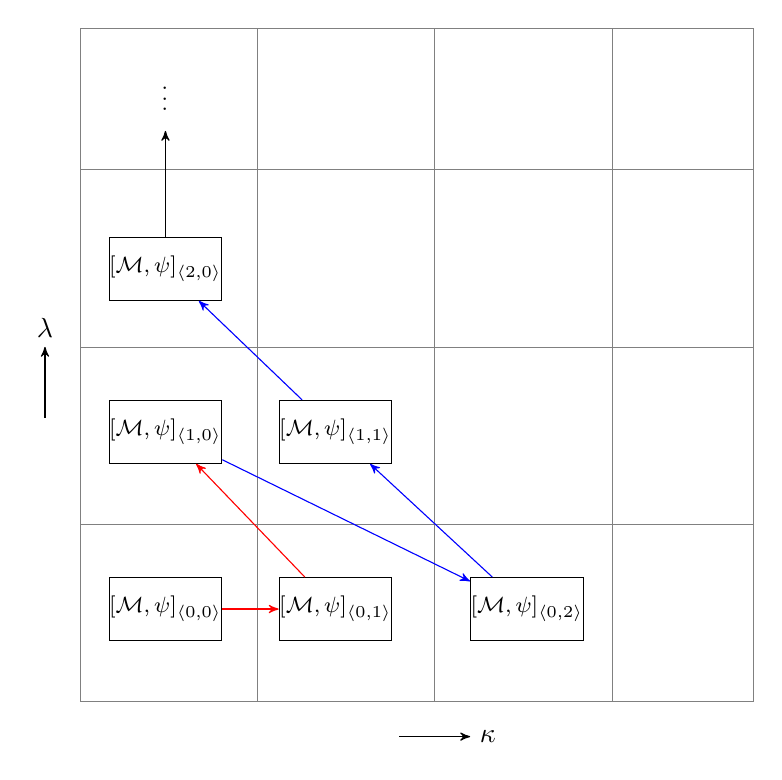
\begin{tikzpicture}[>=stealth,scale=0.9] 
			\tikzset{
	%Define standard arrow tip
	>=stealth',
	%Define style for boxes
	punkt/.style={
		rectangle,
		rounded corners,
		draw=black, very thick,
		text width=8.5em,
		minimum height=2em,
		text centered},
	% Define arrow style
	pil/.style={
		->,
		thick,
		shorten <=2pt,
		shorten >=2pt,}
}
\tikzstyle{aldecision} = [diamond, draw, fill=blue!20, text width=4.5em, text badly centered, node distance=2.5cm, inner sep=0pt]
\tikzstyle{alblock} = [rectangle, draw, fill=blue!20, text width=5em, text centered, rounded corners, minimum height=4em]
\tikzstyle{line} = [draw, very thick, color=black!50, -latex']
\tikzstyle{allibrary} = [draw, ellipse,fill=red!20, node distance=2.5cm, minimum height=2em]


	\foreach \i in {0,2.5,5,7.5,9.5} {
		\draw[gray,very thin] (0,\i) -- (9.5,\i);
		\draw[gray,very thin] (\i,0) -- (\i,9.5);
	}
	\draw[->] (-.5,4) -- (-.5,5) node[above] {$\lambda$};
	\draw[->] (4.5,-0.5) -- (5.5,-0.5) node[right] {$\kappa $};
	
	\begin{scope}[every node/.style={
		circle,draw,
		minimum size=.8cm,
		align=center,
		font=\footnotesize,
		inner sep=0pt
	}]
	
	%column lambda=0
	\node[rectangle] at (1.2,1.3) (00) {$[\mathcal{M},\psi]_{\langle 0,0\rangle}$}; 
	\node[rectangle] at (1.2,3.8) (10) {$[\mathcal{M},\psi]_{\langle 1,0\rangle}$}; 
	\node[rectangle] at (1.2,6.1) (20) {$[\mathcal{M},\psi]_{\langle 2,0\rangle}$};
	\node[rectangle,draw=none,rotate=90] at (1.2,8.5) (30) {$\cdots$};
	%column lambda=1  
	\node[rectangle] at (3.6,1.3) (01) {$[\mathcal{M},\psi]_{\langle 0,1\rangle}$};
	\node[rectangle] at (3.6,3.8) (11) {$[\mathcal{M},\psi]_{\langle 1,1\rangle}$};
	%\node[rectangle] at (3.6,6.1) (21) {$(M,\psi)_{(2,1)}$};
%	\node[rectangle,draw=none,rotate=90] at (3.6,6.1) (21) {$\cdots$};
	%\node[rectangle,draw=none] at (3.6,8.5) (31) {$\cdots$};
	%column lambda=2 
	\node[rectangle] at (6.3,1.3) (02) {$[\mathcal{M},\psi]_{\langle0,2\rangle}$};
	%\node[rectangle] at (6.3,3.8) (12) {$(M,\psi)_{(1,2)}$};
%	\node[rectangle,draw=none] at (6.3,3.8) (12) {$\cdots$};
	%\node[rectangle] at (6.3,6.1) (22) {$(M,\psi)_{(2,2)}$}; 
	%column lambda=3
%	\node[rectangle,draw=none] at (8.5,1.3) (03) {$\cdots$}; 
	%\node[rectangle,draw=none] at (8.5,3.8) (13) {$\cdots$};
	
	%k=1 unfolding arrows
%	\draw[red,->] (00) -- (10);
	\draw[red,->] (00) -- (01);
	\draw[red,->] (01) -- (10);
	%k=2 unfolding arrows
	\draw[blue,->] (10) -- (02);
	\draw[blue,->] (02) -- (11);	
	\draw[blue,->] (11) -- (20);  
	%k=3 unfolding arrows
	\draw[->] (20) -- (30); 
%	\draw[->] (11) -- (21); 
%	\draw[->] (11) -- (12);
%	\draw[->] (02) -- (03);

	%\draw[->] (12) -- (13);
	%\draw[->] (21) -- (31);
   

	
	\end{scope}
	
	\end{tikzpicture}

}
    \caption{Unfolding of the encoded formula  $[\mathcal{M},\psi]_{(\lambda,\kappa)}$ with respect to $\lambda$ (execution steps) and $\kappa$ (number of tokens)}

    \label{2dbmcunfolding}
\end{figure}

%


\subsubsection{Unfolding the encoded formula}

The unfolding of the formula $[\mathcal{M},\psi]_{\langle\lambda,\kappa\rangle}$ for each $k$ with respect to $\lambda$ (execution steps) and $\kappa$ (number of tokens), upto $k=2$ is depicted pictorially in Fig.~\ref{2dbmcunfolding}. Initially, when $k=\lambda+\kappa=0$, $k=0$ (bound), $\lambda=0$ (time instance), $\kappa=0$ (number of clients), the formula $[\mathcal{M},\psi]_{\langle 0,0\rangle}$ is evaluated. If this is found to be satisfiable, then, a witness is obtained, and we are done. If not, in the next macro-step of the unfolding, where $k=\lambda+\kappa=1$, there are possibly two micro-steps to be explored $\langle\lambda,\kappa\rangle=\langle 0,1\rangle$ and $\langle\lambda,\kappa\rangle=\langle 1,0\rangle$. First, $\kappa$ is incremented and the formula $[\mathcal{M},\psi]_{\langle 0,1\rangle}$ is evaluated. If this found to be unsatisfiable, $\lambda$ is incremented and the formula $[\mathcal{M},\psi]_{\langle 1,0\rangle}$ is evaluated. In each micro-step of the unfolding, either $\lambda$ or $\kappa$ are incremented, and the resulting formula is verified. The Fig.~\ref{2dbmcunfolding} represents one among many possible ways of exploring the state space in the system.



\section{DCModelchecker : A tool to verify Unbounded PNs}

DCModelChecker 1.0 and DCModelChecker 2.0 perform $2D$-BMC of Petri nets using the logic {\LC}. The key difference between the two tools is in the semantics used for the nets. DCModelChecker 1.0~\cite{Zen2DBMC} can verify {\LC} properties with interleaving semantics. We incrementally extended DCModelChecker 1.0 by adding support for true concurrent semantics to the tool, to obtain DCModelChecker 2.0~\cite{Zen2DBMCv2} which supports both. In the rest of this chapter, when we mention tool, we refer to DCModelChecker 2.0. We give the architecture and the overview of the tool in Section~\ref{sec:arch}. We describe the workflow in Section~\ref{sec:workflow}, and in Section~\ref{sec:experiments}, we report the experiments. The experiments are easily reproducible by directly executing the scripts in our artifact~\cite{Zen2DBMCv2}.

\subsection{Architecture}\label{sec:arch}

The general architecture of the tool is shown in Fig.~\ref{fig:dc2arch}. The tool has two primary inputs- system description in standard \acrfull{PNML}~\cite{HillahKPT10} format and the property to be tested expressed in {\LC}. PNML is based on the \acrfull{XML}, which lends itself to interoperability between tools, while ensuring readability. We employ the \acrfull{ANTLR}~\cite{ANTLRParrF11} tool for parsing the two inputs.
We obtain industrial and academic benchmarks from \acrfull{MCC}~\cite{MCC}. Additionally, we handcraft some Petri net inputs using a Petri net Editor~\cite{PNWolfgang,BerthomieuV06}. We make use of both types of benchmarks, for comparative testing. While several Petri net verification tools perform bounded model checking,
ours is unique in the model checking strategy, displaying
the counterexample and useful in particular for verifying temporal properties and invariants of unbounded client-server systems.




\begin{figure}[!ht]
    \begin{minipage}{0.5\textwidth}
        \centering

        \scalebox{0.5}{\tikzset{
	%Define standard arrow tip
	>=stealth',
	%Define style for boxes
	punkt/.style={
		rectangle,
		rounded corners,
		draw=black, very thick,
		text width=8.5em,
		minimum height=2em,
		text centered},
	% Define arrow style
	pil/.style={
		->,
		thick,
		shorten <=2pt,
		shorten >=2pt,}
}
\tikzstyle{aldecision} = [diamond, draw, fill=blue!20,
text width=4.5em, text badly centered, node distance=2.5cm, inner sep=0pt]
\tikzstyle{alblock} = [rectangle, draw, fill=blue!20,
text width=5em, text centered, rounded corners, minimum height=4em]
\tikzstyle{line} = [draw, very thick, color=black!50, -latex']
\tikzstyle{allibrary} = [draw, ellipse,fill=red!20, node distance=2.5cm,
minimum height=2em]	
\begin{tikzpicture}[node distance = 5em, auto, fit label/.style={yshift={(height("#1")+4pt)/2},
inner ysep={(height("#1")+8pt)/2}, label={[anchor=north,font=\itshape]north:#1}}]
	
	\node [ node distance=2em, xshift=-3em,fill=green!20] (property) {Property Formula};
	\node [ node distance=2em, below of=property, yshift=-1em, fill=green!20] (sysdesc) {System Description};
	\node [alblock, node distance=7em, text width=7em,right of=property,yshift=-1em, xshift=4em] (ppm) {Pre-Processing\\ Module};

	\node [alblock, node distance=7em, right of=ppm, xshift=1em, minimum width=4em] (tool) {$2D$- BMC Module};

	
	\node [allibrary, right of= tool,xshift=1em,rotate=90](z3){Z3 Solver};

	\node [ node distance=2em, below of=tool,yshift=-2em,,xshift=-2em, fill=green!20] (sat) {sat + trace};
	\node [ node distance=2em, right of=sat,  xshift=3em,fill=green!20] (unsat) {unsat};


	\path [line] (sysdesc) -- (ppm);
	\path [line] (property) -- (ppm);

	\path [line] (ppm) -- (tool);


	\path [line] (z3) -- (tool);
	\path [line] (tool) -- (z3);
	\path [line] (tool) -- (sat);
	\path [line] (tool) -- (unsat);
	\path [line] (unsat) --([xshift=2em]unsat.east) -- ([xshift=1em,yshift=-1em]tool.east) -- (tool);

	
\end{tikzpicture}
}
        \caption{DCModelChecker  2.0 architecture}
        \label{fig:dc2arch}

    \end{minipage}
    \begin{minipage}{0.5\textwidth}
        \centering

        \scalebox{0.5}{\tikzset{
	%Define standard arrow tip
	>=stealth',
	%Define style for boxes
	punkt/.style={
		rectangle,
		rounded corners,
		draw=black, very thick,
		text width=8.5em,
		minimum height=2em,
		text centered},
	% Define arrow style
	pil/.style={
		->,
		thick,
		shorten <=2pt,
		shorten >=2pt,}
}
\tikzstyle{aldecision} = [diamond, draw, fill=blue!20,
text width=4.5em, text badly centered, node distance=2.5cm, inner sep=0pt]
\tikzstyle{alblock} = [rectangle, draw, fill=blue!20,
text width=5em, text centered, rounded corners, minimum height=4em]
\tikzstyle{line} = [draw, very thick, color=black!50, -latex']
\tikzstyle{allibrary} = [draw, ellipse,fill=red!20, node distance=2.5cm,
minimum height=2em]	
\begin{tikzpicture}[node distance = 5em, auto, fit label/.style={yshift={(height("#1")+4pt)/2},
inner ysep={(height("#1")+8pt)/2}, label={[anchor=north,font=\itshape]north:#1}}]
	
		\node [ node distance=2em,  yshift=-1em, fill=green!20,text width=5em] (inputexpr) {Input \\Expression};
	
	\node [ node distance=2em, below of=inputexpr,yshift=-4em,fill=green!20] (grammar) {Grammar};


	\node [alblock, node distance=5em, text width=5em,right of=inputexpr, xshift=4em, minimum width=5em] (lexer) {Lexer +\\Parser};
	\node [alblock, node distance=4em, below of=lexer, yshift=-2em, text width = 7em, minimum height=3em] (antlrtool) {ANTLR tool};
	\node [alblock, node distance=4em, right of=lexer,xshift=4em] (parsetree) {parse tree};

	\begin{scope}
	\node [draw=black!50, minimum width=10em, fit={(lexer)  ([yshift=1em]lexer.north)},
	label={[anchor=north,font=\itshape]north:Language Recognizer}] (lr) {};


	\end{scope}


	\node [alblock, node distance=3.5em, right of=parsetree,xshift=4em, text width=5em] (listener) {Listener\\Walker};
	
%	\node [alblock, node distance=5em, text width = 4 em, right of=listener,,xshift=4em] (ptree) {output tree};
	
	\node [ node distance=3em,  text width = 4 em, right of=listener,xshift=4em, fill=green!20] (ptree) {output tree};
	
	\node [allibrary,node distance=12em, above of= parsetree,yshift=-5em,xshift=1em](arl){ANTLR Runtime Library};
		
	\node[fit=(antlrtool)(lr)(parsetree)(listener),draw,minimum height=14em, label={[anchor=south,font=\itshape]south:Pre-Processing Module}] (ppm){};




	\path [line] (inputexpr) -- (lexer);
	\path [line] (lexer) -- (parsetree);
	\path [line] (parsetree) -- (listener);
	\path [line] (listener) -- (ptree);
	\path [line,dashed] (arl)--(lr);
	\path [line,dashed] (lr)--(arl);
	\path [line,dashed] (arl)--(listener);
	\path [line,dashed] (listener)--(arl);


	\path [line] (grammar) -- (antlrtool);
	\path [line] (antlrtool) -- (lr);
	\path [line] (antlrtool.east) -| (listener.south);
		%\path [line] (antlrtool.east)-- ([yshift=-0.5em]lr.west);
		%\path [line] (antlrtool)|- (listener.west);
	
%	\path [line] (z3) -- (tool);
%	\path [line] (tool) -- (z3);
%	\path [line] (tool) -- (sat);
%	\path [line] (tool) -- (unsat);
%	\path [line] (unsat) --([xshift=2em]unsat.east) -- ([xshift=1em,yshift=-1em]tool.east) -- (tool);

	
\end{tikzpicture}
}
        \caption{Pre-Processing the model and formula using ANTLR}
        \label{ANTLRflow}

    \end{minipage}
\end{figure}




First, the two inputs are fed to the pre-processing module and consequently to the DCModelChecker 2.0 tool. The objective of the pre-processing module is to read and validate the two inputs.
We make use of ANTLR to achieve this.
We give the grammar of the nets and properties to the tool so that it can recognize it against its respective grammar as shown in
Fig.~\ref{ANTLRflow}. ANTLR generates a parser for that language that can automatically build parse trees representing how a grammar matches the input.
The parse trees can be walked to construct the required data structures.
We have hand coded the grammar for the PNML format of both
types and the grammar of {\LC}, to be used by ANTLR. This is explained in detail in Sec.~\ref{sec:preprocess}.


The tool reads the output of the pre-processing module and checks if the model satisfies the property or not. We make use of the Z3 SAT/SMT Solver~\cite{MouraB08}, to solve the encoded formula and give us a result of unsatisfiable, or satisfiable with a counterexample trace. If unsatisfiable, the tool can increment the bound and look further, until the external termination bound is hit, according to the BMC algorithm. We chose Z3, for its wide industrial applications, developer community support, and ease of use. The detailed workflow is discussed in the subsequent section.

\subsection{Workflow}\label{sec:workflow}


\begin{figure}[!ht]
    \begin{minipage}{0.35\textwidth}
        \centering

        \scalebox{0.6}{\tikzset{
	%Define standard arrow tip
	>=stealth',
	%Define style for boxes
	punkt/.style={
		rectangle,
		rounded corners,
		draw=black, very thick,
		text width=8.5em,
		minimum height=2em,
		text centered},
	% Define arrow style
	pil/.style={
		->,
		thick,
		shorten <=2pt,
		shorten >=2pt,}
}
\tikzstyle{aldecision} = [diamond, draw, fill=blue!20,
text width=4.5em, text badly centered, node distance=2.5cm, inner sep=0pt]
\tikzstyle{alblock} = [rectangle, draw, fill=blue!20,
text width=5em, text centered, rounded corners, minimum height=4em]
\tikzstyle{line} = [draw, very thick, color=black!50, -latex']
\tikzstyle{allibrary} = [draw, ellipse,fill=red!20, node distance=2.5cm,
minimum height=2em]		
		
\begin{tikzpicture}[node distance = 5em, auto]
\node [node distance=5em,text width = 5em,fill=green!20] (negate) {Negated property $\psi$};
\node [left of=negate,text width=8em,xshift=-4em,text width = 5em,fill=green!20] (readip) {System Description (M) and bound};

\node [aldecision,below of=negate,text width=10em, node distance=14em] (decide0) {At $k=0$,\\ $\lambda=0,~\kappa=0$\\ Is $[\mathcal{M},\psi]_{(0,0)}$ SAT?};
\node [allibrary, right of=negate, ,xshift=1em] (Z3k0) {Z3};
\node [text width=8em,left of=decide0,xshift=-8em,text width = 8em,fill=green!20] (counterex0) {Counter example found at $k=0$. EXIT};
\node [allibrary, below of=decide0, node distance=12em,fill=green!20] (nocounterex0) {A};
			
% Draw edges
\path [line] (readip) -- (decide0);
\path [line] (negate) -- (decide0);
\path [line,dashed] (Z3k0) -- (decide0);
\path [line,dashed] (decide0) -- (Z3k0);
			
\path [line] (decide0) -- node [near start, color=black] {Yes} (counterex0);
			
\path [line] (decide0) -- node [, color=black,text width=10em,left] {No. Counter example is not found at $k=0$}(nocounterex0);		
			
\end{tikzpicture}
}
        \caption{Workflow for $k=0$}
        \label{fig:work0}

    \end{minipage}\hfill
    \begin{minipage}{0.65\textwidth}
        \centering
        \scalebox{0.6}{\tikzset{
	%Define standard arrow tip
	>=stealth',
	%Define style for boxes
	punkt/.style={
		rectangle,
		rounded corners,
		draw=black, very thick,
		text width=8.5em,
		minimum height=2em,
		text centered},
	% Define arrow style
	pil/.style={
		->,
		thick,
		shorten <=2pt,
		shorten >=2pt,}
}
\tikzstyle{aldecision} = [diamond, draw, fill=blue!20,
text width=4.5em, text badly centered, node distance=2.5cm, inner sep=0pt]
\tikzstyle{alblock} = [rectangle, draw, fill=blue!20,
text width=5em, text centered, rounded corners, minimum height=4em]
\tikzstyle{line} = [draw, very thick, color=black!50, -latex']
\tikzstyle{allibrary} = [draw, ellipse,fill=red!20, node distance=2.5cm,
minimum height=2em]		
\begin{tikzpicture}[node distance = 5em, auto]
\node [allibrary, below of=decide0, node distance=12em,fill=green!20] (nocounterex0) {A};
\node [alblock,text width=12em,below of=nocounterex0] (k1) {If  $k <$ bound \\Assign $k=1$\\Else EXIT};
\node [allibrary, right of=k1,xshift=6em] (Z3k0) {Z3};
\node [aldecision,below of=k1,text width=10em, node distance=12em] (decidek) {At $k=1$,\\$\lambda = 0,\kappa = 1 $\\ Is $[\mathcal{M},\psi]_{(0,1)}$ SAT?};
\node [left of=decidek,xshift=-8em,text width = 8em,fill=green!20] (sat10) {Counter example found at $k=1$ $\lambda = 0,~\kappa = 1$. EXIT};

\path [line] (nocounterex0) -- (k1);
\path [line] (k1) -- (decidek);
\path [line,dashed] (Z3k0) |- (decidek);
\path [line,dashed] (decidek) -| (Z3k0);
		
\path [line] (decidek) -- (sat10);
\path [line] (decidek) -- node [near start, color=black] {Yes} (sat10);
		

\node [aldecision,below of=decidek,text width=10em, node distance=18em] (decidek0l1) {At $k=1$,\\$\lambda = 1,\kappa = 0 $\\ Is $[\mathcal{M},\psi]_{(1,0)}$ SAT?};
\path [line] (decidek) -- node [left,near start, color=black,text width=14em] {No. For $k=1$, explore other $\lambda,\kappa$ values.} (decidek0l1);
\path [line,dashed] (Z3k0) |- (decidek0l1);
\path [line,dashed] (decidek0l1) -| (Z3k0);
		
\node [left of=decidek0l1,xshift=-8em,text width = 8em,fill=green!20] (satk0l1) {Counter example found at $k=1$ $\lambda = 1, \kappa = 0$. EXIT};
		
\path [line] (decidek0l1) -- (satk0l1);
\path [line] (decidek0l1) -- node [near start, color=black] {Yes} (satk0l1);

\node [alblock, below of =decidek0l1, text width=8em, yshift=-6em,node distance = 8em] (k2) {If  $k <$ bound\\Assign $k=2$\\And Continue\\Else EXIT};
\path [line] (decidek0l1) -- node [left,near start, color=black,text width=2em] {No} (k2);
\node [allibrary, right of=k2, node distance=10em,fill=green!20] (B) {B};	
\path [line] (k2) -- (B);
\end{tikzpicture}
}
        \caption{Workflow for $k=1$}
        \label{fig:work1}

    \end{minipage}
\end{figure}


The system description $M$, the property formula $\phi$, and external termination bound $k$ are given to us. First, we negate the property, $\psi=\neg \phi$. Note that the negation normal form of $\psi$ is always used in the BMC process. For the bound $k=0$ and the corresponding micro-step
$\langle\lambda,\kappa\rangle=\langle 0,0\rangle$, we construct the formula $[M,\psi]_{\langle 0,0\rangle}$ and feed it to the solver. If the above formula is satisfiable, the property $\phi$ is violated in the initial configuration and we have a {\bf witness} at $k=0$ and we can stop our search. If the base case is unsatisfiable, we consider the next micro-step $\langle \lambda,\kappa\rangle$ -- with the bound $k=\lambda+\kappa=1$ -- and
construct the formula $[M,\psi]_{\langle \lambda,\kappa\rangle}$
and feed it to the solver. If this formula is satisfiable, the property
$\phi$ is violated for $k=\lambda+\kappa$ and we have a {\bf witness} for
this $k$ and we can stop our search. Otherwise, we may continue with the
next micro-step $\langle \lambda',\kappa'\rangle$ and so on. The order in
which the micro-steps are considered is illustrated in Fig.~\ref{2dbmcunfolding}. We have depicted the workflow only up to $k=1$ in Fig.~\ref{fig:work1}. In practice, for the property $\phi$, we search until we have considered all micro-steps for the termination
bound $k$. As expected, for the given model and bound $100$ (i.e, when parameter $k$ reaches $100$) it is observed that a counterexample is not found, hence we terminate. This means that the property holds for all traces of the model up to the length $100$.



\subsection{Pre-processing Petri nets}\label{sec:preprocess}

In order to build a verification tool that uses Petri nets, we require a standard way of representation. While, various Petri net verification tools exist, recently, the most widely accepted standard is the \gls{PNML}. PNML is based on the Extensible Markup Language, or XML for short, which lends itself to interoperability between tools, while ensuring readability. We employ the \gls{ANTLR} for parsing the PNML input. This tool was chosen, since it will also enable us to pre-process the various extensions to Petri nets (cf. Chapter.~\ref{chmodels}) and the various logic specifications(cf. Chapter.~\ref{chlogics}). This module is also available as an open source tool~\cite{dicosmoprince24}.

The tools discussed and built as part of this research work are compatible with any Petri net verification/analysis tools that use the PNML format. Additionally, one may also use existing graphical tools to visualise the Petri nets, limited only by the size of the Petri net~\cite{PNWolfgang}. This decision was made early in the work, to enable reuse of the prototypes and modules built in the tool chain by other research groups and to ensure reproducibility of results.\footnote{It is noteworthy, that when this research was submitted to Petri net tool venues, the tool was awarded the reproducibility badge, however as the tool paper itself was not accepted, it is not being displayed alongside.} We list down the actual \textbf{lexer} and \textbf{parser} grammars that were used to pre-process the nets in the following section.

\subsection*{Lexer rules: }
First, we name the following set of rules, such that we can refer to in the parsing phase:

\begin{lstlisting}
lexer grammar PNMLLexer;
\end{lstlisting}


Consider the following rule that recognizes the escape sequences for tab spaces, carriage return and new line respectively and skips over them when they occur in the input file (PNML file).

\begin{lstlisting}
S           :   [ \t\r\n]+               -> skip ;
\end{lstlisting}

The PNML format is a type of markup file which contains tags. We have the following rules to identify the open, close and comment tags; the digits and text:
\begin{lstlisting}[multicols=2]
COMMENT     :   '<!--' .*? '-->'  -> skip;
SPECIAL_OPEN:   '<?'          -> pushMode(INSIDE) ;
OPEN        :   '<'           -> pushMode(INSIDE) ;
DIGIT       :   [0-9]+ ;
TEXT        :   ~[<&]+ ; //16 bit char except < and &
mode INSIDE;
CLOSE       :   '>'          -> popMode ;
SPECIAL_CLOSE:  '?>'         -> popMode ;
SLASH_CLOSE :   '/>'         -> popMode ;
\end{lstlisting}
We have rules to tokenize the keywords and special characters used in the PNML file:
\begin{lstlisting}[multicols=2]
SLASH       :   '/' ;
EQUALS      :   '=' ;
QUOTE       :   '"' ;
SQUOTE      :   '\'' ;
PLACE       :   'place' ;
TRANSITION  :   'transition' ;
ARC         :   'arc';
INITIAL     :   'initialMarking' ;
INSCRIPTION :   'inscription' ;
TEXTTAG     :   'text' ;
USCORE      :   '_' ;
SOURCE      :   'source' ;
TARGET      :   'target' ;
ID          :   'id' ;
STRING      :   '"' ~[<"]* '"'
            |   '\'' ~[<']* '\'';
\end{lstlisting}
We have a special set of rules for the name tag. The name consists of an alphabet and may be succeded by any combination of digits, alphabets and special symbols (hyphen, underscore, dot), as allowed by the Petri net graphical analysis tool that we used~\cite{PNWolfgang}.
\begin{lstlisting}
Name        :   NameStartChar NameChar* ;
NameChar    :   NameStartChar
            |   '-' | '_' | '.' | DIGIT
            |   '\u00B7'
            |   '\u0300'..'\u036F'
            |   '\u203F'..'\u2040';
NameStartChar  :   [:a-zA-Z]
            |   '\u2070'..'\u218F'
            |   '\u2C00'..'\u2FEF'
            |   '\u3001'..'\uD7FF'
            |   '\uF900'..'\uFDCF'
            |   '\uFDF0'..'\uFFFD';
\end{lstlisting}

\subsection*{Parser rules: }

Now that we have the lexer rules that can identify and tokenize the input, in this section, we write the the parser rules which will be used by ANTLR to construct the parse tree from the valid input and throw errors if any.

First, we set the specific vocabulary of the parser as \textbf{PNMLLexer} (the set of lexer rules we defined above):

\begin{lstlisting}
parser grammar PNMLParser;
options {
    tokenVocab = PNMLLexer;
}
\end{lstlisting}

A valid PNML file contains a header followed by valid elements:

\begin{lstlisting}
doc: header element;
\end{lstlisting}
An element may be either an open tag followed by a close tag or an empty tag, each containing its name and possibly containing a set of attributes. There may be open tags for exactly one of the predefined keywords such as place, transition etc. Notice that it is not possible to define just a close tag using these set of rules. If such an input exists, our tool parses the PNML file and invalidates it by throwing a suitable error.
\begin{lstlisting}
header: '<?' Name attribute* '?>';
element:
       '<' Name attribute* '>' (
        place
        | transition
        | arc
        | element
        | textTagDigit
        | textTag
        | TEXT
        )* '<' '/' Name '>'
        | '<' Name attribute* '/>';
\end{lstlisting}


The place tag contains a mandatory identifier attribute and may contain details to represent the initial marking or special text for parsing.
\begin{lstlisting}
place: '<' 'place' 'id' '=' STRING '>' (initial | element | TEXT)* '<' '/' 'place' '>';
\end{lstlisting}


The rule for parsing the initial marking:
\begin{lstlisting}
initial:
    '<' INITIAL '>' (textTagDigit | textTag | element | TEXT)* '<' '/' INITIAL '>';
\end{lstlisting}

The rule for parsing transitions, with a mandatory identifier.
\begin{lstlisting}
transition:
    '<' 'transition' 'id' '=' STRING '>' (element | TEXT)* '<' '/' 'transition' '>';
\end{lstlisting}
The rule to recognize arcs from a place/transition to transition/place along with their identifiers.
\begin{lstlisting}
arc:
    '<' 'arc' 'id' '=' STRING source target '>' (
        inscription
        | element
        | TEXT
    )* '<' '/' 'arc' '>'
    | '<' 'arc' 'id' '=' STRING source target '/>';
source: 'source' '=' STRING;
target: 'target' '=' STRING;
\end{lstlisting}
Some additional rules to parse the text and specify the type of net for validation:
\begin{lstlisting}
inscription:
    '<' INSCRIPTION '>' (textTagDigit | textTag | element | TEXT)* '<' '/' INSCRIPTION '>';
textTagDigit: '<' TEXTTAG '>' DIGIT '<' '/' TEXTTAG '>';
textTag: '<' TEXTTAG '>' TEXT '<' '/' TEXTTAG '>';
attribute: ('id' | Name) '=' STRING;
\end{lstlisting}

Similarly, the rules are written to validate the logic {\LC} as well and are available in our artifact. As illustrated, in Fig.~\ref{fig:dc2arch}, given a valid system description in a PNML file and a valid specification  which are validated by the pre-processing module, the $2D$-BMC algorithm verifies the specification using Z3 and produces a counterexample trace or times out. In the next section, we look at the experiments conducted on our bounded model checking tool.

\section{Benchmarks and Comparisons}\label{sec:experiments}
In this section, we detail the experimental evaluation of DCModelChecker 2.0. The goals of our evaluation are to demonstrate: (1) the correctness of results returned by DCModelChecker 2.0 in comparison with the state-of-the-art ITS-Tools~\cite{ITSMCC} (2) the comparison of DCModelChecker 2.0 against DCModelChecker 1.0 on similar FireabilityCardinality properties which are not verifiable by tools in the MCC (3) verification of Unbounded Petri nets in comparison with other tools (4) the strength of DCModelChecker 2.0 is in additionally verifying invariants specified in {\LC} which are not verifiable by tools in the MCC nor DCModelChecker 1.0. To replicate the experiments and plots, a collection of simple shell and python scripts are publicly available in our artifact~\cite{Zen2DBMCv2}.

\noindent\textbf{Benchmarks:}
In the first set of experiments described in Section~\ref{exp:compits} we consider benchmark models from the MCC~\cite{MCC} and translated the LTLFireability properties into {\LC}. In our second set of experiments  in Section~\ref{exp:compv1v2}, we make use of the MCC benchmark models and write the properties containing both fireability and cardinality constraints for those models, which are not expressible in the language of MCC. In the third set of experiments, we make use of synthetic unbounded Petri nets~\cite{AmatDH22}. The fourth experiment demonstrates verification of invariants using the unbounded client-server system benchmark (APS) using DCModelChecker 2.0.

\subsection{Experiment 1: Computing the Tool Confidence and Verification of LTLFireability properties - DCModelChecker 2.0 vs the state-of-the-art tool}\label{exp:compits}

To compute the Tool Confidence,  22 benchmarks from the MCC were verified using DCModelChecker 2.0 and compared against the state-of-the-art model checking tool ITS-Tools~\cite{ITSMCC}. ITS-Tools has 100 \% tool confidence~\cite{CompResultMCC22}. We compare against only this tool since (at the time of experimentation) ITS-Tools was the MCC winner in the LTL Fireability category. Since the purpose of this experiment was to evaluate the tool confidence, it would not make any difference to compare against more than one tool.
The comparative experiments were performed with a timeout of $3600$ seconds.


\noindent\textbf{Evaluation Criteria:}
ITS-Tools returns True when the property holds true and False when the property does not hold. DCModelChecker 2.0 however, returns a satisfying counterexample to the negation of the property when the property does not hold. When DCModelChecker 2.0 returns UNSAT, it means that the property holds up to the given bound, and that the property may become false at a greater bound. Hence, for comparison, we may categorize the results of both tools as shown in Table~\ref{table:categoryresults}.\begin{table}[]
    \centering
    \resizebox{0.7\columnwidth}{!}{

        \begin{tabular}{p{10pt}c|cc|}
            \cline{3-4}
                                                                                                      &                                                                    & \multicolumn{2}{c|}{\begin{tabular}[c]{@{}c@{}}ITS Tools\end{tabular}}                                                                                                                                                                        \\ \cline{3-4}
                                                                                                      &                                                                    & \multicolumn{1}{c|}{\begin{tabular}[c]{@{}c@{}}True\end{tabular}}                                                          & \begin{tabular}[c]{@{}c@{}}False\end{tabular}                                                                    \\ \hline
            \multicolumn{1}{|c|}{\multirow{2}{*}[18pt]{\rotatebox[origin=c]{90}{DCModelChecker 2.0}}} & \begin{tabular}[c]{@{}c@{}}SAT\\ Property is False\end{tabular}    & \multicolumn{1}{c|}{\begin{tabular}[c]{@{}c@{}}\\A\\ Erroneous output by\\ DCModelChecker \\$\mid A \mid =7$\end{tabular}} & \begin{tabular}[c]{@{}c@{}}\\B\\ Both tools agree\\ on the property being false \\$\mid B \mid =87$\end{tabular} \\[26pt] \cline{2-4}
            \multicolumn{1}{|c|}{}                                                                    & \begin{tabular}[c]{@{}c@{}}\\UNSAT\\ Property is True\end{tabular} & \multicolumn{1}{c|}{\begin{tabular}[c]{@{}c@{}}C \\$\mid C \mid =72$\end{tabular}}                                         & \begin{tabular}[c]{@{}c@{}}D \\$\mid D \mid =179$\end{tabular}                                                   \\ \hline
        \end{tabular}
    }
    \caption{Experiment 1: Categorization of LTLFireability results.}
    \label{table:categoryresults}

\end{table}


The instances in category A are those false positive properties where DCModelChecker 2.0 returned a counterexample, whereas ITS-Tools returned false. The instances in category B are those where both tools agreed that the property was false, this is particularly significant since it gives the correctness of DCModelChecker 2.0. The instances in category C are those where DCModelChecker 2.0 returns UNSAT and ITS-Tools returns true. The instances in category D are those where DCModelChecker 2.0 returns UNSAT and ITS-Tools returns false. Those instances in categories C and D may become false at a greater bound, hence we do not conclusively take them into account.
We consider only the properties that fall in category A and B for computing the confidence ratio. This is similar to the MCC tool confidence computation~\cite{RulesMCC22} which excludes those values that are not computed by the tool. The Confidence of a tool is a value $C_{tool} \in [0,1]$, where 1 denotes that the tool returns the correct result that is agreed upon by atleast 3 participating tools and 0 denotes that the tool never returns the commonly agreed result (otherwise referred to as trusted values). In the LTL Formulas examination category, ITS-Tools has a tool confidence of 100\%,  $C_{ITS-Tools}= 1$. Hence, it is sufficient to compare DCModelChecker 2. 0 against ITS-Tools to check for the correctness of the results. The $C_{tool}$ is computed as follows:

\begin{equation}
    C_{tool} = \frac{\mid V_{tool}\mid}{\mid V \mid}
\end{equation}

\noindent where $\mid V\mid $ is the number of trusted values, which we obtain from ITS-Tools. $\mid V_{tool} \mid$ is the number of results obtained by DCModelChecker 2.0 within the set of trusted values, such that $V \subseteq V_{tool}$. For Experiment 1, comparing LTL Fireability properties of DCModelChecker and ITS-Tools, we obtained the following tool confidence $C_{DCModelChecker}= \frac{\mid A \mid}{\mid A + B \mid} = 0.90$. The underlying $2D$-BMC strategy is not complete. % As part of future work, we would like to establish completeness criteria for the same.
\subsection{Experiment 2: Verification of FireabilityCardinality properties DCModelChecker 1.0 vs DCModelChecker 2.0}\label{exp:compv1v2}

In this set of experiments, DCModelChecker 1.0 and DCModelChecker 2.0 are compared on similar properties. Here, $20$ benchmarks from the MCC have been considered and their properties expressed  in $\mathcal{L}_{C}$~\cite{2dbmctr22} for verification by DCModelChecker 1.0 and their equivalent {\LC} properties for verification by DCModelChecker 2.0 respectively. The logic {\LC} is strictly more expressive than logic $\mathcal{L}_{C}$. It is to be noted that the languages $\mathcal{L}_{C}$  and {\LC} are not equivalent to the logic language used in the MCC. Hence, we have given $16$ synthetic properties called FireabilityCardinality properties, derived from the LTLFireability and LTLCardinality properties from the MCC.

We introduced the set of FireabilityCardinality properties as a combination of the LTLFireability and LTLCardinality properties. For instance, $G (F(t_0) \land F (\#p_1 >999)) $, which is a conjunction of the temporal property describing the firing of transition $t_0$ and the counting property with place $p_1$.

\begin{figure}[h]
    \centering
    \scalebox{0.4}{\includegraphics{figures/FCPlots/Angiogenesis-PT-01_FCPlot.eps}}
    \caption{Experiment 2: Verification of FireabilityCardinality Properties with bound 5 and 10}
    \label{FCAngioPlot}


\end{figure}



For each of these 20 benchmarks, DCModelChecker 2.0 was pitted against DCModelChecker 1.0 to verify a set of 16 FireabilityCardinality properties for each model, totalling 320 properties and 1280 runs with a timeout of $3600$ seconds each. The execution times (seconds) are plotted as separate line plots for bounds 5 and 10. As a sample, 16 properties were verified for the model Angiogenesis-PT-01 as shown in Fig~\ref{FCAngioPlot}. Each instance represents a FireabilityCardinality property. If the property is false and the tool returns a counterexample trace, it is depicted by a $\bullet$ and the symbol $\times$ denotes that the tool returned unsatisfiable (indicating that the property may be false at a greater bound). In Fig~\ref{FCAngioPlot}, we can observe that for bound 5 (blue line), out of the 16 properties, 5 properties were false. On increasing the bound to 10, we obtain 3 new counterexample traces (corresponding to properties 5, 14 and 15) as more search space is explored by the tool, which also takes more time. This trend is observed in all models in our experiment, when the bound is increased, new counterexamples may be found by tool. The execution times of DCModelChecker 2.0 and DCModelChecker 1.0 are comparable. We observe that DCModelChecker2.0 is better in the sense of falsification of properties (not in terms of execution times), which can be seen from the plots such as the CircadianClock-PT-000001 model, where in property 4, DCModelChecker1.0 (at bound 5 and 10) says unsat, whereas, DCModelChecker2.0 (at bound 10) gives a satisfying counterexample trace. It is important to note that for each property both tools agree on the SAT/ UNSAT answers returned by them. The plots depicting the experiments follow.

\begin{table}[]
\begin{tabular}{cc}
 %Row1
  \includegraphics[width=.5\linewidth]{figures/FCPlots/Angiogenesis-PT-01_FCPlot.eps}&
   \includegraphics[width=.5\linewidth]{figures/FCPlots/CircadianClock-PT-000001_FCPlot.eps} \\
  \end{tabular}    
 %Row2
 \begin{tabular}{cc}
 \includegraphics[width=.5\linewidth]{figures/FCPlots/Dekker-PT-010_FCPlot.eps}&
  \includegraphics[width=.5\linewidth]{figures/FCPlots/Diffusion2D-PT-D05N010_FCPlot.eps}\\
 \end{tabular}    
\end{table}




\begin{table}[]
  \begin{tabular}{cc}
   \includegraphics[width=.5\linewidth]{figures/FCPlots/Eratosthenes-PT-010_FCPlot.eps} &
    \includegraphics[width=.5\linewidth]{figures/FCPlots/ERK-PT-000001_FCPlot.eps}  \\
 \end{tabular}    

 %Row3
 \begin{tabular}{cc}
  \includegraphics[width=.5\linewidth]{figures/FCPlots/FMS-PT-00002_FCPlot.eps}&
   \includegraphics[width=.5\linewidth]{figures/FCPlots/GPPP-PT-C0001N0000000001_FCPlot.eps} \\
 \end{tabular}    

   %row
   \begin{tabular}{cc}
    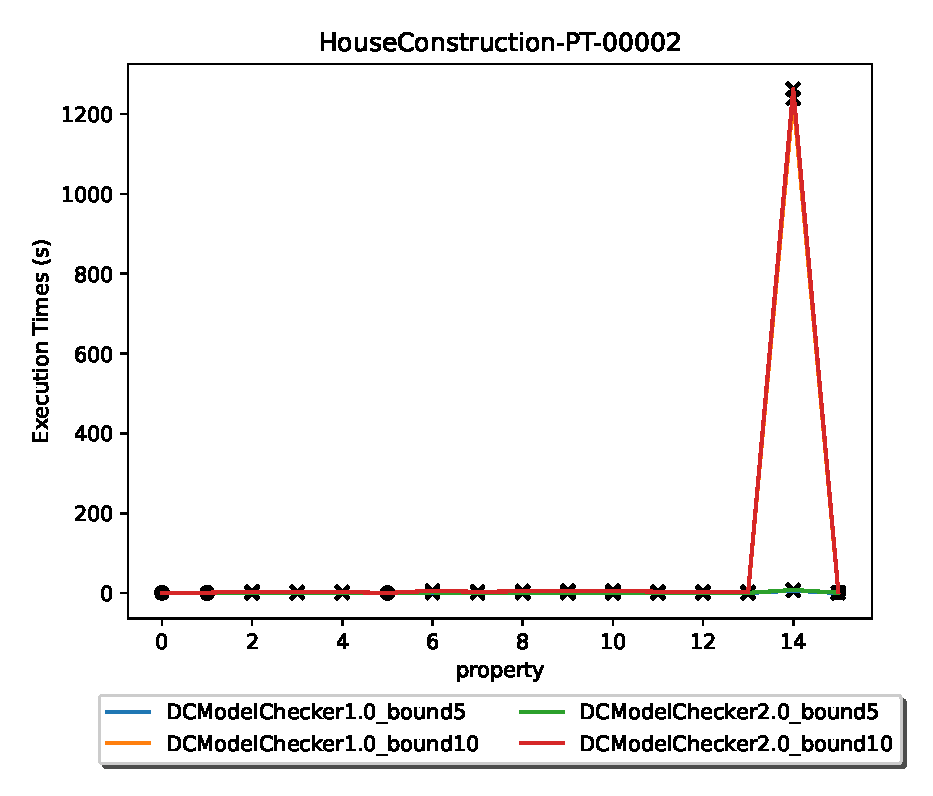
\includegraphics[width=.5\linewidth]{figures/FCPlots/HouseConstruction-PT-00002_FCPlot.eps} &
    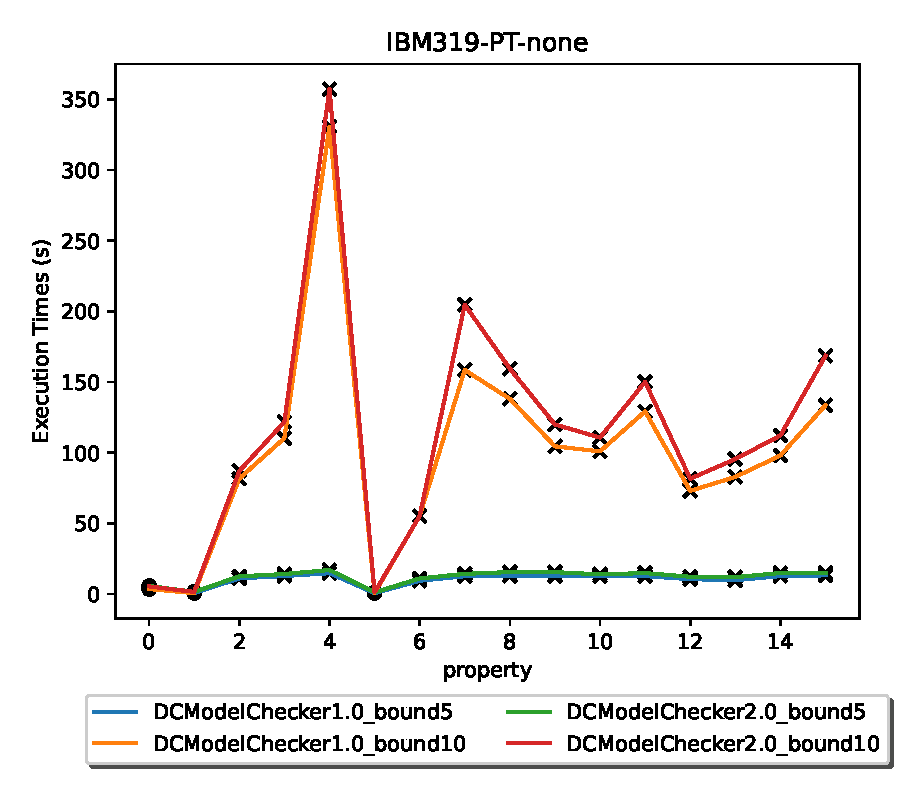
\includegraphics[width=.5\linewidth]{figures/FCPlots/IBM319-PT-none_FCPlot.eps}  \\
   %\includegraphics[width=.5\linewidth]{figures/FCPlots/HypercubeGrid-PT-C3K4P4B12_FCPlot.eps}\\
 \end{tabular}    
  %row
  %\begin{tabular}{cc}
  % \includegraphics[width=.5\linewidth]{figures/FCPlots/HypertorusGrid-PT-d2k1p8b00_FCPlot.eps} &
  %  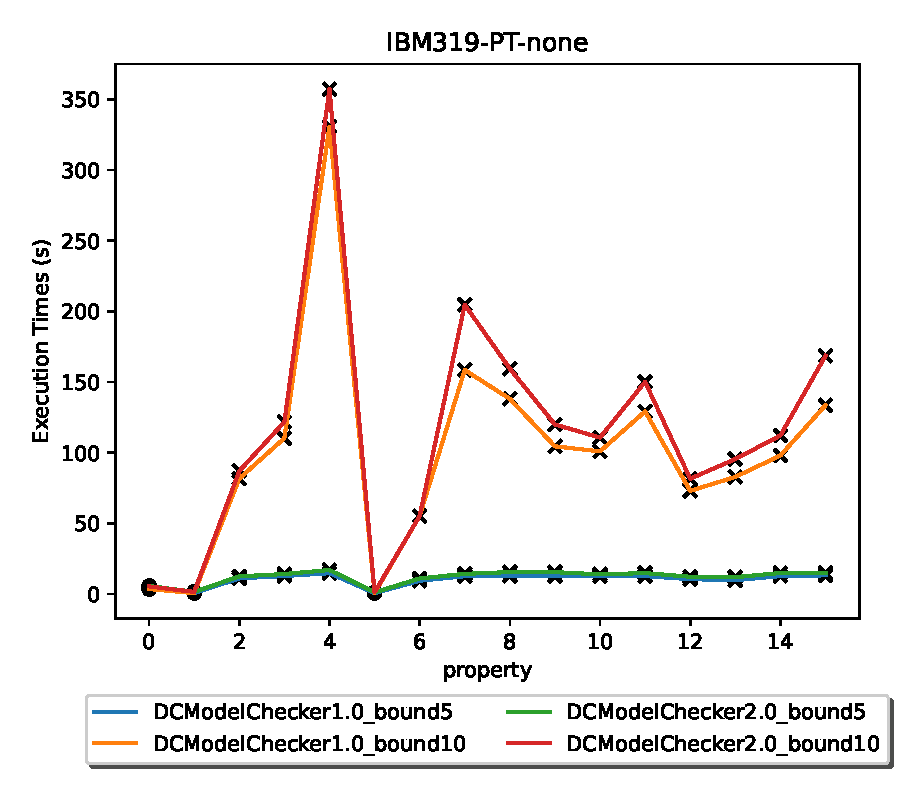
\includegraphics[width=.5\linewidth]{figures/FCPlots/IBM319-PT-none_FCPlot.eps}  \\
 %\end{tabular}    
\end{table}

\begin{table}[]
 %Row5
 \begin{tabular}{cc}
  \includegraphics[width=.5\linewidth]{figures/FCPlots/IBM703-PT-none_FCPlot.eps}&
   \includegraphics[width=.5\linewidth]{figures/FCPlots/IBM5964-PT-none_FCPlot.eps} \\
\end{tabular}    
   %
   \begin{tabular}{cc}
    \includegraphics[width=.5\linewidth]{figures/FCPlots/IOTPpurchase-PT-C01M01P01D01_FCPlot.eps}  &
    \includegraphics[width=.5\linewidth]{figures/FCPlots/Kanban-PT-00005_FCPlot.eps}\\
\end{tabular}    
\end{table}


\begin{table}[]
\begin{tabular}{cc}
   \includegraphics[width=.5\linewidth]{figures/FCPlots/MAPK-PT-00008_FCPlot.eps} &
    \includegraphics[width=.5\linewidth]{figures/FCPlots/PaceMaker-PT-none_FCPlot.eps}  \\
 \end{tabular}    


 %Row7
 \begin{tabular}{cc}
  \includegraphics[width=.5\linewidth]{figures/FCPlots/SimpleLoadBal-PT-02_FCPlot.eps}&
  \includegraphics[width=.5\linewidth]{figures/FCPlots/TCPcondis-PT-05_FCPlot.eps}  \\
\end{tabular}    
\begin{tabular}{cc}
\includegraphics[width=.5\linewidth]{figures/FCPlots/TriangularGrid-PT-1200_FCPlot.eps}&
  \includegraphics[width=.5\linewidth]{figures/FCPlots/CircularTrains-PT-012_FCPlot.eps}\\

\end{tabular}
\end{table}

\newpage
\subsection{Experiment 3: Verification of Unbounded Petri nets}\label{exp:upn}
To quote Amat et al, ``It is difficult to find benchmarks for unbounded Petri nets''~\cite{AmatDH22}. The strength of DCModelChecker 2.0 lies in verifying unbounded Petri nets. Since, MCC benchmarks are bounded~\cite{AmatDH22}, we make use of the unbounded Petri nets given by~\cite{NAmatGH} and verify LTLFireability properties in comparison with DCModelChecker 1.0~\cite{Zen2DBMC}, ITS-Tools~\cite{ITSMCC}. The results of these experiments are in Table~\ref{table:unboundedpn}, and~\cite{Zen2DBMC}. Each property that was verified is false. In each case it was observed that DCModelChecker 2.0 and DCModelChecker 1.0 returned that the property is false and additionally gave a counterexample trace, whereas ITS-Tools and Tapaal~\cite{DavidJJJMS12} returned that the property is false. Here, we compared our tools against both ITS-Tools and Tapaal, since Tapaal is faster than ITS-Tools and we give a comparative perspective of our tool's performance. In Section~\ref{exp:upn}, we verified LTLFireability properties of unbounded Petri nets which were all found to be false (while specifying the bound as $5$).
The properties are described in Table~\ref{table:upnprop}. The detailed output is available in the artifact~\cite{Zen2DBMC}.

\begin{table}[ht]
    \centering
    \resizebox{0.7\columnwidth}{!}{

        \begin{tabular}{|c|c|c|c|c|}
            \hline
            \multirow{2}{*}{Model} & \multicolumn{4}{c|}{Execution Times(ms)}                                                   \\
            \cline{2-5}
                                   & DCModelChecker 1.0   (bound =5)                    & DCModelChecker 2.0 (bound =5) & ITS-Tools & Tapaal         \\
            \hline
            Parity                 & \textbf{0.010}                           & 0.40               & 0.933     & 0.02           \\
            \hline
            PGCD                   & \textbf{0.019}                           & 0.98               & 1.487     & 0.07           \\
            \hline
            Process                & 0.033                                    & 0.85               & 1.201     & \textbf{1e-05} \\
            \hline
            CryptoMiner            & 0.036                                    & 0.64               & 0.957     & \textbf{7e-06} \\
            \hline
            Murphy                 & 0.031                                    & 0.83               & 1.161     & \textbf{8e-06} \\
            \hline
        \end{tabular}
    }
    \caption{Results of Experiment 3}
    \label{table:unboundedpn}

\end{table}

\begin{table}
    \centering

    \begin{tabular}{|l|l|}
        \hline
        \textbf{Model} & \textbf{Property}                 \\
        \hline
        Parity         & $\neg(t_0 U t_1)$                 \\
        \hline
        PGCD           & $\neg GF(t_0 U t_1)$              \\
        \hline
        Process        & $\neg F(t_0 U t_1)$               \\
        \hline
        CryptoMiner    & $\neg F(\text{OB } U \text{ GH})$ \\
        \hline
        Murphy         & $\neg F(t_1 U t_4)$               \\
        \hline
    \end{tabular}
    \caption{Experiment 3: List of properties verified on unbounded nets}
    \label{table:upnprop}

\end{table}
\subsection{Experiment 4: Verification of invariants for unbounded client-server systems using DCModelChecker 2.0}\label{exp:aps}

We have additionally verified client-server properties specified in the {\LC} language on our synthetic benchmark APS, against {\LC} specifications. These cannot be verified using DCModelChecker 1.0~\cite{Zen2DBMC}. The specifications are available in our artifact~\cite{Zen2DBMCv2}. Our experiments demonstrate that DCModelChecker 2.0 has an advantage over DCModelChecker 1.0 in being able to additionally verify invariants. And it can be added to the arsenal of BMC tools for Petri nets.
%In Section~\ref{sec:rel} we discuss the contributions of other tools that verify the properties of Petri nets.

\subsection{Related Petri net verification tools}
There are several tools such as KREACH~\cite{DixonL20}, Petrinizer~\cite{EsparzaLMMN14}, QCOVER~\cite{BlondinFHH16}, ICOVER~\cite{GeffroyLS18} verifying specific classes of properties like reachability and coverability of Petri nets. Recently, in~\cite{AmatBD21,AmatDH22} the generalized reachability of Petri net is encoded into a BMC problem and solved using SMT solvers. However, BMC for unbounded Petri nets with true concurrency and LTL properties while leveraging the power of SMT Solvers remained unexplored until now. DCModelChecker bridges this gap.


The MCC has attracted many tools for formal verification of concurrent systems that use a portfolio approach. In particular, we looked at ITS-Tools~\cite{ITSMCC} which implements structural reduction techniques~\cite{Mieg20} and uses a layer of SMT when solving LTL. Moreover, it does not perform BMC. While ITS-Tools is much faster on bounded nets (MCC benchmarks) it gives only binary answers (sat or unsat). From our experiments, on a subset of unbounded nets, while Tapaal is faster, it also gives binary answers. On the contrary, our tool preserves the original Petri net structure and additionally gives a counterexample trace which is useful in bug finding in systems.

\subsubsection*{Conclusion}\label{ssec:conclltltool}
In this chapter, we discussed the first of its kind verification tool for checking properties of unbounded client server systems using $2D$-BMC.

In Experiment 1 (Sec.~\ref{exp:compits}) where we compute the tool confidence as well as verify LTLFireability properties, we compare against only ITS-Tools since (at the time of experimentation) ITS-Tools was the MCC winner in the LTL Fireability category. Since the purpose of this experiment was to evaluate the tool confidence, it would not make any difference to compare against more than one tool, apart from the winning tool. In Experiment 3 (Sec.~\ref{exp:upn}) where we verify unbounded Petri nets which is not a category in the contest, we compared our tools against both ITS-Tools and Tapaal, since Tapaal is faster than ITS-Tools and we give a comparative perspective of our tool's performance.

We would like to have an optimal encoding of the PN with true concurrent semantics, such that we can better understand the advantage of true concurrent semantics. This will be done as part of future work.

Next, we shall look at an extension of the Petri net, called $\nu$-net and a different and richer logic, a variant of First Order logic, to express a different set of specifications of unbounded client server systems in the upcoming chapter.
\chapter{First Order LTL Tool with Monodic restriction}\label{chmfotl}
\section{FO LTL over Petri nets with names}

Formal verification of Petri nets is well studied. In practice, many communication protocols, services and applications are client-server systems. These systems can be modeled as Petri nets and verified using existing tools. However, these tools are not specifically suited for unbounded client-server systems as they do not allow the user to explicitly specify client and server properties as well as their unboundedness. Traditional logics such as LTL or CTL are not suitable for expressing these properties either. It is necessary to find suitable logics to express properties of unbounded client-server systems where the number of clients is not known a priori and the clients are distinguishable. To specify the properties of such systems, we consider a one variable fragment of \acrfull{MFOTL}, called {\Lstar} which is described in detail in Section~\ref{sec:mlogic}. We propose a restriction on the $\nu$-net to model the unbounded client server system. This model has been described earlier in Sec.~\ref{sec:apscasestudy}.


\begin{recallfigure}[ht]{fig:APS}
  \begin{center}
    \scalebox{0.8}{\input{figures/2_fig_aps_vnet_v2}}
    \caption{Recall the restricted $\nu$-net modeling an unbounded client-server system}
  \end{center}
\end{recallfigure}

\section{Tool and Implementation}

The verification tool follows the same underlying architecture as DCModelChecker 2.0, where we employ Z3 to perform SMT queries using Linear Integer Arithmetic theory. The key difference is in the choice of logic and model.  We make use of ANTLR to pre-process the $\nu$-net, as previously discussed. In the rest of this chapter, we refer to the {\Lstar} properties of the APS case study (See.~\ref{sec:apscasestudy}). Since this is a first of its kind, there are no similar tools to compare the results of the model checker. However, we can see from the liveness windows that the counterexample or UNSAT obtained from the tool are justified.

\begin{recallfigure}[!ht]{fig:dc2arch}
  \centering
  \scalebox{0.5}{\tikzset{
	%Define standard arrow tip
	>=stealth',
	%Define style for boxes
	punkt/.style={
		rectangle,
		rounded corners,
		draw=black, very thick,
		text width=8.5em,
		minimum height=2em,
		text centered},
	% Define arrow style
	pil/.style={
		->,
		thick,
		shorten <=2pt,
		shorten >=2pt,}
}
\tikzstyle{aldecision} = [diamond, draw, fill=blue!20,
text width=4.5em, text badly centered, node distance=2.5cm, inner sep=0pt]
\tikzstyle{alblock} = [rectangle, draw, fill=blue!20,
text width=5em, text centered, rounded corners, minimum height=4em]
\tikzstyle{line} = [draw, very thick, color=black!50, -latex']
\tikzstyle{allibrary} = [draw, ellipse,fill=red!20, node distance=2.5cm,
minimum height=2em]	
\begin{tikzpicture}[node distance = 5em, auto, fit label/.style={yshift={(height("#1")+4pt)/2},
inner ysep={(height("#1")+8pt)/2}, label={[anchor=north,font=\itshape]north:#1}}]
	
	\node [ node distance=2em, xshift=-3em,fill=green!20] (property) {Property Formula};
	\node [ node distance=2em, below of=property, yshift=-1em, fill=green!20] (sysdesc) {System Description};
	\node [alblock, node distance=7em, text width=7em,right of=property,yshift=-1em, xshift=4em] (ppm) {Pre-Processing\\ Module};

	\node [alblock, node distance=7em, right of=ppm, xshift=1em, minimum width=4em] (tool) {$2D$- BMC Module};

	
	\node [allibrary, right of= tool,xshift=1em,rotate=90](z3){Z3 Solver};

	\node [ node distance=2em, below of=tool,yshift=-2em,,xshift=-2em, fill=green!20] (sat) {sat + trace};
	\node [ node distance=2em, right of=sat,  xshift=3em,fill=green!20] (unsat) {unsat};


	\path [line] (sysdesc) -- (ppm);
	\path [line] (property) -- (ppm);

	\path [line] (ppm) -- (tool);


	\path [line] (z3) -- (tool);
	\path [line] (tool) -- (z3);
	\path [line] (tool) -- (sat);
	\path [line] (tool) -- (unsat);
	\path [line] (unsat) --([xshift=2em]unsat.east) -- ([xshift=1em,yshift=-1em]tool.east) -- (tool);

	
\end{tikzpicture}
}
  \caption{DCModelChecker  3.0 architecture}
\end{recallfigure}


\subsection*{Recognizing {\Lstar} properties}
A valid {\Lstar} formula has the server formula $sformula$ which contains the client formula $cformula$ as a sub formula.
\begin{lstlisting}
grammar mlogic;
input :  sformula EOF;
sformula
    : sorop | sandop | simpliesop | suntilop | snotop
        | snextop | sdiamondop | sboxop ;
cformula
    : (corop | candop | cimpliesop | cuntilop | cnotop
        | cnextop | cdiamondop | cboxop );
\end{lstlisting}
We define the server temporal modalities:
\begin{lstlisting}
sorop
    : (exists | forall )(place_x | snotop )
       OR
      ssubformula;
sandop
    : (exists | forall )(place_x | snotop )
       AND
      ssubformula;
simpliesop
    :  (exists | forall )(place_x | snotop )
       IMPLIES
      ssubformula;
suntilop
      : (exists | forall ) (place_x | snotop | snextop | sdiamondop | sboxop)
       SUNTIL
      ssubformula;

snotop
    : NOT (exists | forall ) ssubformula;
snextop
    : SNEXT (exists | forall ) ssubformula;
sdiamondop
    : SDIAMOND (exists | forall ) ssubformula;
sboxop
    : SBOX (exists | forall )  ssubformula;

ssubformula : LPAREN (cformula| place_x | snotop | snextop | sdiamondop
                      | sboxop | sandop | sorop | simpliesop | simpliesop) RPAREN;
\end{lstlisting}
Consequently, we define the client temporal modalities:
\begin{lstlisting}
corop
    : (place_x | cnotop | cnextop | cdiamondop | cboxop)
        OR
        csubformula;
candop
    : (place_x | cnotop | cnextop | cdiamondop | cboxop)
        AND
        csubformula;
cimpliesop
    : (place_x | cnotop | cnextop | cdiamondop | cboxop)
        IMPLIES
        csubformula;
cuntilop
    : (place_x | cnotop | cnextop | cdiamondop | cboxop)
        CUNTIL
        csubformula;
cnotop
    : NOT csubformula;
cnextop
    : CNEXT csubformula;
cdiamondop
    : CDIAMOND csubformula;
cboxop
    : CBOX csubformula;

csubformula: LPAREN (place_x | cnotop | cnextop | cdiamondop
                     | cboxop | candop | corop | cimpliesop | cuntilop) RPAREN;
\end{lstlisting}
We provide the rules governing quantifiers:
\begin{lstlisting}
exists : EXISTS VAR;
forall : FORALL VAR;
place_x : PLACE DIGIT LPAREN VAR RPAREN;
\end{lstlisting}
We recognize the valid tokens for the various temporal modalities and operators:
\begin{lstlisting}
EXISTS: 'E';
FORALL: 'V';
PLACE : 'p';
NOT : '~';
SNEXT : 'X_s';
SDIAMOND : 'F_s';
SBOX : 'G_s';
CNEXT : 'X_c';
CDIAMOND : 'F_c';
CBOX : 'G_c';
OR : '|';
AND : '&';
IMPLIES : '%';
SUNTIL : 'U_s';
CUNTIL : 'U_c';
\end{lstlisting}
We recognize the valid symbols such as paranthesis and identifiers and spaces:
\begin{lstlisting}
LPAREN : '(';
RPAREN : ')';
NAME : '\'' ~[']+ '\'';
VAR: [a-z];
DIGIT : '-'?[0-9]+;
ENDLINE : ('\r\n'|'\n'|'\r')+ -> skip;
WHITESPACE : [\t ]+ -> skip;
\end{lstlisting}

Instead of providing separate parser and lexer rules, we provide the grammar for recognizing {\Lstar} in one shot. Using the above rules, we validate the {\Lstar} specifications in the accompanying tool.
\subsection{Observations}\label{ssec:obsr}
We list down some observations about the logic {\Lstar} which supplement our
understanding of the language.

\begin{dfn}{Ghost Interval }
  Given a temporal property of a client, whose right boundary is
  $\lambda '$ such that the $\lambda ' < \lambda$. There is a ghost interval between
  $\lambda$ and $\lambda'$ where the formula $\alpha$ need not be asserted.
\end{dfn}



\begin{recallfigure}[ht]{fig:livewindows}
  \centering
  \scalebox{0.7}{\begin{ganttchart}[
vgrid,hgrid,
%inline,
progress label text=\relax,
x unit=10mm,
% title top shift=0,
title height=1,
foobar top shift=.15,
foobar height=.70
]{0}{5}
%\gantttitlelist{0,...,5}{1}\\
 \textganttbar{Client 1}{$p_{PR}$}{0}{0}  \textganttbar{}{$p_{OP}$}{1}{1} \textganttbar{}{$p_{ES}$}{2}{2} \\
  \textganttbar{Client 2}{$p_{PR}$}{1}{1}  \textganttbar{}{$p_{PU}$}{2}{2}  \textganttbar{}{$p_{EU}$}{3}{3}\\
   \textganttbar{Client 3}{$p_{PR}$}{3}{3} \textganttbar{}{$p_{PR}$}{4}{4}\textganttbar{}{$p_{PR}$}{5}{5}\\
   \textganttbar{Client 4}{$p_{PR}$}{4}{4} \textganttbar{}{$p_{PR}$}{5}{5}
   \begin{scope}[yshift=0.33cm]
    \draw[->] (0,0) -- (6.5,0);
    
    \draw ([yshift=-3pt]0,0) -- ++([yshift=6pt]0,0) node[xshift=45pt, yshift=15pt, above] {time instance $\rightarrow$};
    
    \draw ([yshift=-3pt]1,0) -- ++([yshift=6pt]0,0) node[xshift=-10pt, above] {$0$};
    \draw ([yshift=-3pt]2,0) -- ++([yshift=6pt]0,0) node[xshift=-10pt, above] {$1$};
    \draw ([yshift=-3pt]3,0) -- ++([yshift=6pt]0,0) node[xshift=-10pt, above] {$2$};
    \draw ([yshift=-3pt]4,0) -- ++([yshift=6pt]0,0) node[xshift=-10pt, above] {$3$};
    \draw ([yshift=-3pt]5,0) -- ++([yshift=6pt]0,0) node[xshift=-10pt, above] {$4$};
    \draw ([yshift=-3pt]6,0) -- ++([yshift=6pt]0,0) node[xshift=-10pt, above] {$\cdots$};
    %\draw ([yshift=-3pt]7,0) -- ++([yshift=6pt]0,0) node[xshift=-10pt, above] {$\cdots$};
\end{scope}
 \end{ganttchart}}
  \caption{Snapshot of the running example $(APS)$ depicting live windows}
\end{recallfigure}

In Fig.~\ref{fig:livewindows}, there is a \emph{ghost interval} for client $1$ between $1$ (right boundary) and $5$ (the bound $\lambda$).\\

Let $\psi_5 = (\forall x) \Big( \mathbf{G}_c \big(parking\_requested(x)
    \mathbf{U}_c~ exit\_successfully(x) \big)\Big)$. In $\psi_5$,
$\mathbf{G}_c$ holds only till the \emph{live window} ends for the corresponding client i.e, this will be asserted only as long as the client is \emph{live}. Similarly, all other client temporal modalities $\mathbf{F}_c$, $\mathbf{U}_c$, and $\mathbf{X}_c$ need not be asserted beyond the \emph{live window} of that particular client.


At any given time, there are as many client lassos as there are clients, which are then combined to
construct the server lasso. For currently \emph{active} clients the right boundary
will be the execution bound $\lambda$.

We list down some of the properties that cannot be expressed in {\Lstar}:
\begin{enumerate}
  \item Consider the property, where there is at least one token in either place $p_{SR}$ or $p_{SB}$ or $p_{RR}$. From the net, $p_{SR}+p_{SB}+p_{RR} = 1$ is an invariant.
        These places represent the server being available, busy and the server rejecting the request.

  \item The following property is not expressible in {\Lstar}: It is always the case that the client request with an identifier (say) $1001$ is rejected.
  \item It is always the case that if the client request is accepted at time instance $x$, then the client exits the parking space at time instance $z$, $z>x$.
        %\item Formulas involving alternating quantifiers are not permitted.
  \item Formulas with quantifiers before server temporal modality are not permitted.

  \item We do not have formulas of type, client $i$ satisfies a formula whereas client $j$ doesn't satisfy the same formula. We do not have equality/inequality to differentiate between the clients. We assume that all clients behave the same way and are of the same type. In the future, this model could be extended to clients of a finite set of types.% in which case properties with equality will be useful to us.

  \item We cannot compare clients in the same state.

        \begin{align*}
          \psi_6 = \mathbf{G}_s ((\exists x)(\exists y)parking\_requested(x) \land parking\_requested(y) \land \\
          \mathbf{F}_c(exit\_successfully (x) \land \mathbf{F}_c (exit\_successfully (y)))
        \end{align*}

  \item Here, there are no free variables either in the scope of $\mathbf{G_s}$ or $\mathbf{F_s}$.
        \begin{align*}
          \text{Let } \psi_7 = \big(\mathbf{G_s} (\exists x)~parking\_requested(x)\big) \land \big(\mathbf{F_s}(\exists y)~parking\_requested(y)\big)
        \end{align*}
  \item[]  The formula $\psi_7$ states that it is always the case that there is a client who has requested parking and eventually, there exists a client who has also requested parking. However, we cannot compare these two clients in our logic.
\end{enumerate}




%It can be observed that there are no free variables in the scope of $\mathbf{G_s}$ and exactly one free variable in the scope of the client modalities. It is also possible to construct {\Lstar} specifications with propositions from $P_s$ and server transitions.
The ease of expressibility of the client and server behaviour is the key motivation behind the logic {\Lstar} which is formally described in Sec.~\ref{sec:mlogic}.

\subsection{Experimental results}\label{ssec:experimentsfotl}
We test the properties of the APS case study (See Sec.~\ref{sec:apscasestudy}) written using {\Lstar} using our open source tool~\cite{zenodomfotl}. The tool provides the detailed counterexample trace when the property is violated. We assume a bound of $5$ for the below experiments in Table.~\ref{tab:experimentsmfotltool}. The properties are present in Sec.~\ref{sec:mlogic}. To the best of our knowledge, there are no known benchmarks for {\Lstar} and $\nu$-nets, hence we create our own $\nu$-net model using a PN editor called Wolfgang and properties in {\Lstar} for our experiments. 
% In order to verify properties of other $\nu$-nets, we create the model using a PN editor called Wolfgang and then specify the properties in {\Lstar}.
\begin{table}[h!]
  \centering
  \caption{Experiments on APS}
  \label{tab:experimentsmfotltool}
  \begin{tabular}{|c|c|c|c|}
    \hline
    Property ID & Nesting Depth of temporal operators & Number of clauses & time (ms) \\
    \hline
    $\psi_1$    & 2                                           & 3                 & 0.32      \\

    \hline
    $\psi_2$    & 2                                           & 2                 & 0.4       \\
    \hline
    $\psi_3$    & 2                                           & 2                 & 0.5       \\
    \hline
    $\psi_4$    & 2                                           & 3                 & 0.38      \\
    \hline
  \end{tabular}
\end{table}

\subsection{Limitations of the tool}\label{ssec:limitationsfotltool}
The current toolchain depends on a PNML Editor, Wolfgang~\cite{PNWolfgang}, which we use to draw the net and mention the arc labels. However, identifiable tokens are not supported by the Wolfgang editor, as it is primarily a Petri net and Colored Petri net simulation tool. Hence, we have to handcraft the $\nu$-net arcs, which is not sustainable when the number of places and transitions are huge.
While there are several tools to model other types of PNs, to the best of our knowledge, there are none that provide a graphical representation of $\nu$-nets. We consider this as a future extension to this work. We would like to perform detailed experiments for various other $\nu$-net models and by varying the nesting depth of the formulas, to identify if it has an impact on the execution times.

While the logic {\Lstar} allows us to reason about distinguishable clients, we cannot describe properties of each individual client. In future, we would like to explore different logics to do the same.
\section{Bounded Semantics of {\Lstar}}\label{ssec:bsem}
We introduce the (unbounded) satisfaction relation $\models_{x}$ with respect to the free variable $x$, where $x$ is used to denote the client names. This relation is not necessary for the BMC tool, but it is useful in Lemma.~\ref{lem:bound}. Hence it is given in Appendix.~\ref{ssec:verif}.

In this section, we describe the bounded semantics of {\Lstar} in order to arrive at the SMT encoding, which is necessary for BMC.
We use $\models^{k}$ as a restriction on $\models$, where $k$ is the bound in the BMC strategy.
To tackle the unbounded number of clients as well as unboundedness in the unfolding of the model, it is necessary to introduce two bounds: $\kappa$ is a bound on the number of clients and $\lambda$ is a bound on the execution steps of the net. The two parameters $\kappa$ and $\lambda$ are independent of each other. Since the runs are bounded, there are atmost $\kappa$ clients in the system, namely CN = $\{0,\ldots ,\kappa-1\}$.

\begin{figure}[!h]
    \begin{minipage}{0.5\textwidth}
        \centering

        \scalebox{0.7}{\begin{ganttchart}[
vgrid,hgrid,
%inline,
progress label text=\relax,
x unit=10mm,
% title top shift=0,
title height=1,
foobar top shift=.15,
foobar height=.70
]{0}{2}
%\gantttitlelist{0,...,5}{1}\\
 \textganttbar{Client 1}{$p_{PR}$}{0}{0}  \textganttbar{}{$p_{OP}$}{1}{1} \textganttbar{}{$p_{OP}$}{2}{2} \\
  \textganttbar{Client 2}{$p_{PR}$}{1}{1}  \textganttbar{}{$p_{PU}$}{2}{2}%  \textganttbar{}{$pc_2$}{3}{3}\\
  % \textganttbar{Client 3}{$pc_1$}{3}{3} \textganttbar{}{$pc_1$}{4}{4}\textganttbar{}{$pc_1$}{5}{5}\\
%   \textganttbar{Client 4}{$pc_1$}{4}{4} \textganttbar{}{$pc_1$}{5}{5}
      \begin{scope}[yshift=0.33cm]
    \draw[-] (0,0) -- (3,0);
    
    %\draw ([yshift=-3pt]0,0) -- ++([yshift=6pt]0,0) node[xshift=-10pt, above] {};
    
    \draw ([yshift=-3pt]0,0) -- ++([yshift=6pt]0,0) node[xshift=45pt, yshift=15pt, above] {time instance $\rightarrow$};

    \draw ([yshift=-3pt]1,0) -- ++([yshift=6pt]0,0) node[xshift=-10pt, above] {$0$};
    \draw ([yshift=-3pt]2,0) -- ++([yshift=6pt]0,0) node[xshift=-10pt, above] {$1$};
    \draw ([yshift=-3pt]3,0) -- ++([yshift=6pt]0,0) node[xshift=-10pt, above] {$2$};
    %\draw ([yshift=-3pt]4,0) -- ++([yshift=6pt]0,0) node[xshift=-10pt, above] {$3$};
   % \draw ([yshift=-3pt]6.5,0) -- ++([yshift=6pt]0,0) node[xshift=-10pt, above] {$\cdots$};
\end{scope}
 \end{ganttchart}}
         \caption{Snapshot at bound = $2$}
    \label{fig:livewindowsline}
  \
    \end{minipage}\hspace{2em}
    \begin{minipage}{0.5\textwidth}
        \centering

        
        \scalebox{0.7}{\input{figures/live_windows_overlap_line_3}}
    \caption{Snapshot at bound = $5$ }
    \label{fig:livewindowsline3}

    \end{minipage}
\end{figure}


\begin{recallfigure}[ht]{fig:loopfreepath}
  \centering
  \scalebox{0.6}{		\begin{tikzpicture}[shorten >=1pt,node distance=2cm,on grid,auto] 
		\node[state] (s)   {}; 
		\node[state,font=\Large] (si) [ right=of s] {$s_i$};
		\node[state] (si1) [ right=of si] {};
		\node[state,font=\Large] (sk) [ right=of si1] {$s_\lambda$};
		\path[->] 
		(s) edge  node {} (si)
		(si) edge  node {} (si1)
		(si1)	edge  node{} (sk);
		\end{tikzpicture}	}
  \caption{Recall the bounded loop-free path of length $\lambda$}
\end{recallfigure}

We describe the bounded semantics of {\Lstar} in two subsections, based on the existence of a loop in the behaviour of the net (in Sec.~\ref{ssec:boundedLoop}) and without a loop (in Sec.~\ref{ssec:boundedloopfree}).
\subsection{Bounded Semantics Without Loop}\label{ssec:boundedloopfree}

First, we describe the bounded semantics without loop as shown in Fig.~\ref{fig:loopfreepath} where $0\leq i \leq \lambda$, where $i$ is the current instance on the bounded path. We introduce $\models^{k}_x$ as an extension of the satisfaction relation $\models^{k}$.% with respect to the free variable $x$, where $x$ is used to denote the client names.%, where the formula is evaluated and $k$ is the bound:

\begin{enumerate}
  \item $M,i\models^{k} q$ iff $q \in \nu_i$.

  \item $M,i\models^{k} \lnot q$ iff $q \not\in \nu_i$.

  \item $M,i \models^{k} (\exists x)\alpha$ iff $\exists a\in CN$, $a \in V_i$ and $M,[x\mapsto a],i\models^{k}_x \alpha$.

  \item[] The above formula is satisfied when there is at least one live client such that $\alpha$ is satisfied in the model at instance $i$ for the particular live client $a$.
    Given $\alpha={pc}_1 \lor {pc}_2$ and the snapshot of the system with the bound $2$ is in Fig.~\ref{fig:livewindowsline}. Here, $CN=\{1,2\}$. At instance $i=0$, model $M$ satisfies formula $\alpha$. Hence, this formula holds true at instance $0$.

  \item $M,i \models^{k} (\forall x)\alpha$ iff $\forall a\in CN$, if $a \in V_i$ then $M,[x\mapsto a],i\models^{k}_x \alpha$.

  \item[] The above formula is satisfied when the $\alpha$ is satisfied in the model at instance $i$ for all live clients in the set $CN$. Given $\alpha={pc}_4$ and Fig.~\ref{fig:livewindowsline}. The model $M$ does not satisfy the formula for all clients, since client $2$ does not satisfy $\alpha$.

  \item $M,i\models^{k} \psi_1\lor\psi_2$ iff $M,i\models^{k} \psi_1$ or $M,i\models^{k} \psi_2$.

  \item $M,i\models^{k} \psi_1\land\psi_2$ iff $M,i\models^{k} \psi_1$ and $M,i\models^{k} \psi_2$.


  \item $M,i\models^{k} \mathbf{X_s}\psi$ iff $
          \begin{cases}
            M,i+1\models^{k} \psi                & \text{if }(i<\lambda) \\
            M,i\not \models^{k}\mathbf{X_s} \psi & \text{otherwise }
          \end{cases}$

  \item[] When instance $i$ is less than the bound $\lambda$, the formula $\psi$ is evaluated at instance $i+1$ else, the formula is unsatisfiable.



  \item $M,i\models^{k} \mathbf{F_s}\psi$ iff $\exists j: i \le j \le\lambda$ , $M,j\models^{k} \psi$.

  \item[] This formula is satisfiable if there is some instance $j$ such that $i \le j \le\lambda$ at which the property $\psi$ holds. Given $\psi= (\exists x){pc}_4$. In Fig.~\ref{fig:livewindowsline}, the formula is unsatisfiable. However, in Fig.~\ref{fig:livewindowsline3}, it is satisfiable at instance $5$, where client $4$ is in local state ${pc}_4$.

  \item $M,i\not\models^{k} \mathbf{G_s} \psi$

  \item[] In the absence of a loop in the bounded run, the above formula is always unsatisfiable, since global server behaviour cannot be evaluated without a loop.

  \item $M,i\models^{k} \psi_1\mathbf{U_s}\psi_2$ iff $\exists j: i \le j \le\lambda$, $M,j\models^{k} \psi_2$ and $\forall j': i \le j' < j: M,j' \models^{k} \psi_1$.

  \item[] This formula is satisfied when formula $\psi_2$ is satisfied at some instance $j$  and for all instances less than $j$, formula $\psi_1$ is satisfied.
    %
    %
    %\newline\newline
    %


  \item $M,[x\mapsto a],i\models^{k}_x p(x)$ iff $\xi_i(a,p)=\top$.

  \item[] This formula is satisfied if the property $p$ is satisfied by live agent $a$ at instance $i$. Here, the free variable $x$ is substituted by the client name $a$.
  \item $M,[x\mapsto a],i\models^{k}_x \lnot \alpha$ iff $M,[x\mapsto a],i\not\models^{k}_x \alpha$.

  \item $M,[x\mapsto a],i\models^{k}_x \alpha\lor \beta$ iff $M,[x\mapsto a],i\models^{k}_x\alpha$ or $M,[x\mapsto a],i\models^{k}_x\beta$.


  \item $M,[x\mapsto a],i\models^{k}_x \alpha\land \beta$ iff $M,[x\mapsto a],i\models^{k}_x\alpha$ and $M,[x\mapsto a],i\models^{k}_x\beta$.

        %\item $M,[x\mapsto a],i\models^{k}_x \mathbf{X}_c\alpha$ if $i<\lambda$ and $a \in V_{i+1}$ then $M,[x\mapsto a],i+1\models^{k}_x \alpha$ else $M,[x\mapsto a],i\not \models^{k}_x \mathbf{X}_c\alpha$. % formatted below


  \item $M,[x\mapsto a],i\models^{k}_x \mathbf{X}_c\alpha$ iff $
          \begin{cases}
            M,[x\mapsto a],i+1\models^{k}_x \alpha                 & \text{if } (i<\lambda \text{ and } a \in V_{i+1}) \\
            M,[x\mapsto a],i\not \models^{k}_x \mathbf{X}_c \alpha & \mbox{otherwise }
          \end{cases}$

  \item[] If the instance $i$ is less than the bound $\lambda$ and the client is a live client at instance $i+1$, then the formula is evaluated at the instance $i+1$ for the live client $a$; else the original formula is not satisfied.

  \item $M,[x\mapsto a],i\models^{k}_x \mathbf{F}_c\alpha$ iff $\exists j: i \le j \le\lambda$, $a\in V_j$ and $M,[x\mapsto a],j\models^{k}_x \alpha$.


  \item[] This formula is satisfiable if there is some instance $j$ such that $i \le j \le\lambda$ at which the property $\alpha$ is satisfied for the client $a$ and the client $a$ is a live client at instance $j$. Given $\alpha={pc}_2$. In Fig.~\ref{fig:livewindowsline} and Fig.~\ref{fig:livewindowsline3}, the formula is satisfiable at instance $1$ due to client $1$.

  \item $M,[x\mapsto a],i \models^{k}_x \mathbf{G}_c\alpha \text{ iff }\\
          \begin{cases}
            M,[x\mapsto a],j \not \models^{k}_x \alpha                           & \text{if }(\forall j> i \text{ and } a\in V_j) \\
            \forall j':i\le j'<j, M,[x\mapsto a],j' \models^{k}_x \alpha         & \text{otherwise }                              \\
            \text{where } j>i \text{ be the least instance where }a \not \in V_j &
          \end{cases}$

  \item[] For all instances $j$ such that $j>i$ if client $a$ is live at instance $j$, the formula is not satisfiable at $j$.
    Let $j$ be the least instance where client $a$ is not live. For all instances $j'$ such that $i\le j'<j$, formula $\alpha$ is evaluated at $j'$.

  \item $M,[x\mapsto a],i\models^{k}_x \alpha\mathbf{U}_c\beta$ iff $\exists j \ge i$, $a\in V_j$,  $M,[x\mapsto a],j\models^{k}_x \beta$, and $\forall j': i \le j'  < j$,  $M,[x\mapsto a],j' \models^{k} \alpha$.


  \item[] This is satisfied when $\beta$ is satisfied at some instance $j$ and client $a$ is a live client at $j$; and for all instances less than $j$, client formula $\alpha$ is satisfied.

\end{enumerate}

Notice that in the bounded semantics equations $15$-$18$, the semantics depend crucially on whether $a$ is a live agent. Similarly, we can describe the bounded semantics with $(\lambda,l)$ - loop similar to the $(k,l)$ - loop in ~\cite{BiereCCSZ03}. As shown in Fig.~\ref{fig:klloop}, $i$ is the current instance on the bounded path, where the formula is evaluated, $\lambda$ is the bound and $l$ is the start position of the loop, where $0\leq i \leq \lambda$ and $0\leq l \leq \lambda$. Consider the following lemma that relates the bounded and unbounded semantics of logic {\Lstar}.



\begin{recallfigure}[ht]{fig:klloop}
  \centering
  \scalebox{0.6}{		\begin{tikzpicture}[shorten >=1pt,node distance=2cm,on grid,auto,minimum size=1em] 
		\node[state] (s)   {}; 
		%\node[state] (s1) [ right=of s] {}; 
		\node[state,font=\Large] (sl) [ right=of s] {$s_l$};		
		\node[state] (sl1) [ right=of sl] {};
		\node[state,font=\Large] (si) [ right=of sl1] {$s_i$};
		\node[state,font=\Large] (sk) [ right=of si] {$s_\lambda$};
		\path[->] 
		(s) edge  node {} (sl)
		%(s1) edge  node {} (sl)
		(sl)	edge  node{} (sl1)
		(sl1)	edge  node{} (si)
		(si)	edge  node{} (sk)
		(sk)	edge [bend right] node {}(sl)	;
		\end{tikzpicture}	}
  \caption{Recall the bounded path with $(\lambda,l)$ - loop}
\end{recallfigure}

\subsection{Bounded Semantics with Loop}\label{ssec:boundedLoop}
We now give the bounded semantics for {\Lstar} with loop as seen in Fig.~\ref{fig:klloop}.
\begin{enumerate}
  \item $M,i\models^{k} q$ iff $q \in \nu_i$.

  \item $M,i\models^{k} \lnot q$ iff $q \not\in \nu_i$.

  \item $M,i \models^{k} (\exists x)\alpha$ iff $\exists a\in CN$, $a \in V_i$ and $M,[x\mapsto a],i\models^{k}_x \alpha$.

  \item $M,i \models^{k} (\forall x)\alpha$ iff $\forall a\in CN$, if $a \in V_i$ then $M,[x\mapsto a],i\models^{k}_x \alpha$.

  \item $M,i\models^{k} \psi_1\lor\psi_2$ iff $M,i\models^{k} \psi_1$ or $M,i\models^{k} \psi_2$.

  \item $M,i\models^{k} \psi_1\land\psi_2$ iff $M,i\models^{k} \psi_1$ and $M,i\models^{k} \psi_2$.


  \item $M,i\models^{k} \mathbf{X_s}\psi$ iff $
          \begin{cases}
            M,i+1\models^{k} \psi & \text{ if } (i <\lambda) \\
            M,l\models^{k} \psi   & \text{otherwise }
          \end{cases}$

  \item[] When instance $i$ is less than the bound $\lambda$, the formula $\psi$ is evaluated at instance $i+1$ else, $\psi$ is evaluated at instance $l$, which is the next instance of $\lambda$.


  \item $M,i\models^{k} \mathbf{F_s}\psi$ iff $\exists j: min(l,i)\le j \le \lambda$, $M,j\models^{k} \psi$.

  \item[] This formula is satisfiable if there is some instance $j$ such that $min(l,i) \le j \le\lambda$, where the formula $\psi$ is satisfied.

  \item $M,i\models^{k} \mathbf{G_s} \psi$ iff $\forall j: min(l,i)\le j \le \lambda$, $M,j\models^{k} \psi$.

  \item[] This formula is satisfiable if for all instances $j$ such that $min(l,i) \le j \le\lambda$, the formula $\psi$ is satisfied in each instance.


  \item $M,i\models^{k} \psi_1\mathbf{U_s}\psi_2 \text{ iff }
          \begin{cases}
            \exists j:i \le j \le \lambda, M,j\models^{k} \psi_2 \text{ and } & \text{ if }(i\le l) \\
            \forall j': i \le j' < j: M,j' \models^{k} \psi_1                 &                     \\
            \exists j: i \le j \le \lambda, M,j\models^{k}\psi_2 \text{ and } & \text{ if } (i> l)  \\
            \forall j': i \le j' <j: M,j' \models^{k} \psi_1                  &                     \\
            \hspace{10em}\text{or}                                            &                     \\ %or
            \exists j: l \le j < i, M,j\models^{k}\psi_2 \text{ and }         &                     \\
            \forall j': l \le j' < j: M,j' \models^{k} \psi_1
          \end{cases}$

  \item[] Consider the two cases:
    \begin{itemize}
      \item If $(i\le l)$, the current instance $i$ is less than or equal to the loop instance $l$, this formula is satisfied when formula $\psi_2$ is satisfied at some instance $j$  such that $i \le j \le \lambda$ and for all instances between $i$ and $j$, formula $\psi_1$ is satisfied.
      \item If $(i> l)$, the formula may be satisfied in either of the two intervals between $i$ to $\lambda$ or between $l$ to $i$. Hence, the formula is satisfied if either of the following is satisfied: formula $\psi_2$ is satisfied at some instance $j$  such that $i \le j \le \lambda$ and for all instances less than $j$, formula $\psi_1$ is satisfied or, formula $\psi_2$ is satisfied at some instance $j$  such that $l \le j < i$ and for all instances between $l$ and $j$, formula $\psi_1$ is satisfied.
    \end{itemize}
    %
    %
  \item $M,[x\mapsto a],i\models^{k}_x p(x)$ iff $\xi_i(a,p)=\top$.

  \item $M,[x\mapsto a],i\models^{k}_x \lnot \alpha$ iff $M,[x\mapsto a],i\not\models^{k}_x \alpha$.

  \item $M,[x\mapsto a],i\models^{k}_x \alpha\lor \beta$ iff $M,[x\mapsto a],i\models^{k}_x\alpha$ or $M,[x\mapsto a],i\models^{k}_x\beta$.


  \item $M,[x\mapsto a],i\models^{k}_x \alpha\land \beta$ iff $M,[x\mapsto a],i\models^{k}_x\alpha$ and $M,[x\mapsto a],i\models^{k}_x\beta$.


  \item $M,[x\mapsto a],i\models^{k}_x \mathbf{X}_c\alpha \text{ iff }
          \begin{cases}
            M,[x\mapsto a],i+1\models^{k}_x \alpha                & \text { if } i <\lambda \text{ and }a \in V_{i+1} \\
            M,[x\mapsto a],l\models^{k}_x \alpha                  & \text{ if } i = \lambda \text{ and }a \in V_{l}   \\
            M,[x\mapsto a],i\not\models^{k}_x \mathbf{X}_c \alpha & \text{ otherwise }
          \end{cases}$
  \item[] When current instance $i$ is less than the bound $\lambda$, and the client $a$ is a live agent at the next instance $i+1$, the formula is evaluated at instance $i+1$ else, in the current instance if the bound $\lambda$ and the client is live at instance $l$, then the formula is evaluated at instance $l$, which is the next instance of $\lambda$. Otherwise, the original formula does not hold.



  \item $M,[x\mapsto a],i\models^{k}_x \mathbf{F}_c\alpha$ iff $\exists j: min(l,i) \le j \le\lambda$ , $a\in V_j$ , $M,[x\mapsto a],j\models^{k}_x \alpha$.


  \item[] This formula is satisfiable if there is some instance $j$ such that $min(l,i) \le j \le\lambda$, and the client $a$ is live at instance $j$, where the formula $\psi$ is satisfied.

  \item $M,[x\mapsto a],i\models^{k}_x \mathbf{G}_c\alpha$ iff $\forall j: min(l,i) \le j \le\lambda$ , $a\in V_j$ , $M,[x\mapsto a],j\models^{k}_x \alpha$.





  \item $M,[x\mapsto a],i\models^{k} \alpha\mathbf{U_c}\beta \text{ iff }\\
          \begin{cases}
            \exists j:i \le j \le \lambda,a\in V_j, M,[x\mapsto a],j\models^{k} \beta \text{ and } & \text{ if }(i\le l) \\
            \forall j': i \le j' < j: M,[x\mapsto a],j' \models^{k} \alpha                         &                     \\
            \exists j: i \le j \le \lambda,a\in V_j, M,[x\mapsto a],j\models^{k}\beta \text{ and } & \text{ if } (i> l)  \\
            \forall j': i \le j' <j: M,[x\mapsto a],j' \models^{k} \alpha                          &                     \\
            \hspace{10em}\text{or}                                                                 &                     \\
            \exists j: l \le j < i$,$a\in V_j, M,[x\mapsto a],j\models^{k}\beta \text{ and }       &                     \\
            \forall j': l \le j' < j, M, [x\mapsto a], j'\models^{k} \alpha.
          \end{cases}$


  \item[] Consider the two cases:
    \begin{itemize}
      \item If $(i\le l)$, the current instance $i$ is less than or equal to the loop instance $l$, and the client $a$ is live at instance $j$ then this formula is satisfied when formula $\psi_2$ is satisfied at some instance $j$  such that $i \le j \le \lambda$ and for all instances between $i$ and $j$, formula $\psi_1$ is satisfied.
      \item If $(i> l)$, the formula may be satisfied in either of the two intervals between $i$ to $\lambda$ or between $l$ to $i$. Hence, the formula is satisfied if either of the following is satisfied: formula $\psi_2$ is satisfied at some instance $j$  such that $i \le j \le \lambda$ and the client $a$ is live at instance $j$ and for all instances less than $j$, formula $\psi_1$ is satisfied or, formula $\psi_2$ is satisfied at some instance $j$ such that $l \le j < i$ and the client $a$ is live at instance $j$ and for all instances between $l$ and $j$, formula $\psi_1$ is satisfied.
    \end{itemize}
\end{enumerate}

The Lemma 1, states that if a LTL formula is satisfied in a bounded run, then it is also satisfied in an unbounded run.
\begin{lemma}[~\cite{BiereCCSZ03}]\label{lem:boundltlbiere}
  Let f be a LTL formula and $\Pi$ be a path then $\Pi \models^{k} f \implies \Pi\models f$.
\end{lemma}


Following this, we state a similar lemma for {\Lstar}:
\begin{lemma}\label{lem:bound}
  Let f be a {\Lstar} formula and $\Pi$ be a path then $\Pi \models^{k}_x f \implies \Pi\models_{x} f$.
\end{lemma}
% Lemma~\ref{lem:bound} is similar to the Lemma 1 in~\cite{BiereCCSZ03}.
% \noindent \textbf{Proof Sketch: } The proof proceeds by performing a case-by-case analysis of the client and server formulae. For instance, consider the server atomic formula $f=q$. It needs to be proved that $\Pi \models^{i}_k q \implies \Pi\models^{i} q$. Consider the left hand side.
% \begin{itemize}
%   \item[-] $\Pi \models^{i}_k q$
%   \item IFF $q \in v_i$ (Using the semantics described in Section~\ref{ssec:bsem})
%   \item[-] IFF $\Pi\models^{i} q$
% \end{itemize}

% Lemma~\ref{lem:bound} is similar to the one in~\cite{BiereCCSZ03} and the complete proof is left to the reader based on the sketch given above.

\begin{thm}
  {\Lstar} is decidable.
\end{thm}
\begin{proof}
  MFOTL is decidable~\cite{HWZ01}.
  {\Lstar} is a syntactic fragment of MFOTL which is monodic and restricted to quantifier rank 1.
\end{proof}

\section{Related Work}\label{sec:relconcl}
An $MFOTL$ formula $\varphi$ is {\sf monodic} if every subformula has at most one free variable, in the scope of $\psi$'s. Decidability is shown by encoding models of a monodic sentence $\varphi$ in structures called {\sf quasimodels} and then expressing the statement ``there exists a quasimodel satisfying a given monodic sentence'' as a monadic second order sentence. In~\cite{HKKWZ}, they show that the monodic fragment is also $EXPSPACE$-complete.
In this work, we propose a one-variable fragment of $MFOTL$, called {\Lstar} for unbounded client-server systems. Additionally, we have provided the bounded semantics which led to the SMT encoding of this logic. The SMT encoding is desirable for implementing a bounded model checking tool where the properties are specified in this logic for unbounded client-server systems.

\noindent\emph{Parametric verification:} In contrast to the BMC approach, there is existing literature on parametric verification such as~\cite{Lowe22}, where authors consider a fixed number of identifiable processes on which safety and deadlock-freedom is verified. %They perform parametric verification by obtaining an upper bound using the view abstraction technique.
In~\cite{DecidableReasoningOOPSLA17}, they work with a decidable fragment of First Order Logic, with a
quantifier prefix $\exists^{\ast}\forall^{\ast}$, popularly known as the Bernays-Sch\"{o}nfinkel-Ramsey Class, where the temporal modalities are not considered in the same manner as in MFOTL. Their goal is to check the inductive invariants for safety and liveness properties, with expert inputs, whereas, ours focuses on automatic, push button verification of properties including safety, liveness and deadlock over unbounded $\nu$-nets without additional user intervention. Another key difference here, is how the fragment that we consider has only one sort, whereas, in~\cite{DecidableReasoningOOPSLA17}, there are many sorts, some of which are bounded due to domain knowledge. %Additionally, they verify the implementation of the Paxos protocol, whereas, we verify the design of the unbounded client server system against its properties. 
In comparison with~\cite{KVW17}, where parametric verification of threshold automata where there are identifiers, our approach allows for an unbounded number of identified processes, without imposing an explicit bound on the number of processes.
%Our approach is different from parametric verification, since the number of clients is unknown apriori, which is in contrast with
In~\cite{LeaderElectionTACAS17,Lowe22,UnboundedMAS16,KVW17} the bounds are predetermined and in~\cite{DecidableReasoningOOPSLA17}, a part of the parameters are predetermined and bounded.

\noindent\emph{Interactive Theorem Proving:} While employing Interactive Theorem Provers or proof systems such as $TLA^+$~\cite{Chen2016,Chand2016,KonnovLSW23}, user expertise and guidance during the verification process, in contrast to BMC approach which is automatic. Recently, in~\cite{KarpMillerCOQ17,KarpMillerMinCovCOQ24}, the interactive theorem prover COQ has been used for verifying the foundational Karp-Miller algorithm for computing the coverability tree. This technique has not been extended yet, to verify Petri net properties.
As part of future work, we would like to build a BMC tool that takes in {\Lstar} specifications for unbounded client-server systems based on the SMT encoding given in this work. Building verification tools for unbounded client-server systems is a non-trivial engineering pursuit. The BMC implementation using {\Lstar} specifications will join the arsenal of tools such as KREACH~\cite{DixonL20}, Petrinizer~\cite{EsparzaLMMN14}, QCOVER~\cite{BlondinFHH16}, ICOVER~\cite{GeffroyLS18} for nets.
We can also have multiple types of clients in the unbounded client-server systems, which may model a richer set of systems. Alongside this, the complexity and decidability of model checking unbounded client-server systems using {\Lstar} specifications is yet to be explored.

\subsubsection*{Conclusion}
In this chapter, we discussed a verification tool for Petri nets with identifiers and a variant of First Order Logic. In the upcoming chapter, we consider Petri nets with nesting and look at suitable temporal properties on them and build a tool to verify them as well.



\begin{subappendices}
   \clearpage
   \section{Appendix: Unbounded semantics of {\Lstar}}\label{ssec:verif}
In this section, we introduce some satisfiability relations with respect to {\Lstar}.
Given a valid model $M=(\nu,V,\xi)$, the satisfiability relations $\models$  and $\models_x$ can be defined, via induction over the structure of the server formulae $\psi\in \Psi$, and client formulae $\alpha\in \Delta$, respectively. 
%  We selectively describe some of the important relations that provide insight into the others.
\begin{enumerate}
  \item $M,i\models q$ iff $q \in \nu_i$.
  \item[] The atomic server formula $q \in P_s$  is satisfied in the model $M$ at instant $i$ if and only if $q$ is a member of the local state of the server $\nu_i$ at instant $i$, where $i \in \mathbb{N}_0$.

  \item $M,i\models \lnot q$ iff $q \not\in \nu_i$.

  \item $M,i \models (\exists x)\alpha$ iff $\exists a\in CN$, $a \in V_i$ and $M,[x\mapsto a],i\models_x \alpha$.
  \item[] The client formula $\alpha$ is satisfied at some instant $i$ if and only if $\alpha$ is satisfied in any of the \emph{live} clients in $V_i$ i.e, for some client $a \in CN$ and the client name $a \in V_i$, where $i \in \mathbb{N}_0$.

  \item $M,i \models (\forall x)\alpha$ iff $\forall a\in CN$, if $a \in V_i$ then $M,[x\mapsto a],i\models_x \alpha$.

  \item $M,i\models \psi_1\lor\psi_2$ iff $M,i\models \psi_1$ or $M,i\models \psi_2$.

  \item $M,i\models \psi_1\land\psi_2$ iff $M,i\models \psi_1$ and $M,i\models \psi_2$.

  \item $M,i\models \mathbf{X_s}\psi$ iff $M,i+1\models \psi$.

  \item $M,i\models \mathbf{F_s}\psi$ iff $\exists j \ge i$, $M,j\models \psi$.
  \item[] The server formula $\mathbf{F_s}\psi$ is satisfied at some instant $i$ if and only if there is some instant $j \ge i$, where the formula $\psi$ holds.

  \item $M,i\models \mathbf{G_s} \psi$ iff $\forall j \ge i$, $M,j\models \psi$.

  \item $M,i\models \psi_1\mathbf{U_s}\psi_2$ iff $\exists j \ge i$, $M,j\models \psi_2$ and $\forall j':i\le j' < j: M,j' \models \psi_1$.

  \item[]

  \item $M,[x\mapsto a],i\models_x p(x)$ iff $\xi_i(a,p)=\top$.

  \item $M,[x\mapsto a],i\models_x \lnot \alpha$ iff $M,[x\mapsto a],i\not\models_x \alpha$.

  \item $M,[x\mapsto a],i\models_x \alpha\lor \beta$ iff $M,[x\mapsto a],i\models_x\alpha$ or $M,[x\mapsto a],i\models_x\beta$.


  \item $M,[x\mapsto a],i\models_x \alpha\land \beta$ iff $M,[x\mapsto a],i\models_x\alpha$ and $M,[x\mapsto a],i\models_x\beta$.

  \item $M,[x\mapsto a],i\models_x \mathbf{X}_c\alpha$ iff $M,[x\mapsto a],i+1\models_x \alpha$ and $a\in V_{i+1}$.

  \item $M,[x\mapsto a],i\models_x \mathbf{F}_c\alpha$ iff $\exists j\ge i$, $a\in V_j$, $M,[x\mapsto a],j\models_x \alpha$ .
  \item[] The client formula $\mathbf{F}_c\alpha$ is satisfied at some instant $i$ if and only if there is some instant $j \ge i$, where the formula $\alpha$ holds in any of the \emph{live} clients in $V_j$.

  \item $M,[x\mapsto a],i\models_x \mathbf{G}_c\alpha$ iff $\forall j\ge i$, $a\in V_j$, $M,[x\mapsto a],j\models_x \alpha$.

  \item $M,[x\mapsto a],i\models_x \alpha\mathbf{U}_c\beta$ iff $\exists j \ge i$, $M,[x\mapsto a],j\models_x \beta$ and $\forall j':i\le j'  < j: M,j' \models \alpha$ and $a\in V_j$.

\end{enumerate}



\end{subappendices}
\chapter{Verification of Elementary Object Systems}\label{cheos}

\section{Introduction}
Imperfections are natural in the context of message passing systems: imperfect communication channels may spontaneously lose, duplicate, or shuffle carried messages or even deliver new unwanted ones. When compared to their perfect counterpart, verification of imperfect systems is usually easier. For example, reachability in Communicating Finite Automata (CFA) over \emph{perfect} (FIFO) channels is undecidable~\cite{brand_communicating_1983}, but it is decidable when the channels are \emph{lossy}~\cite{hutchison_mixing_2008} (messages may be non-deterministically lost and never delivered) or \emph{unordered}~\cite{georgiou_network_2021} (the message sending and reception order may be different).
The same principle generally holds even outside CFA. Specifically, two counter machines can encode Turing Machines~\cite{MinskyComputationFinite,dershowitz_lets_2021} and suffer from undecidable reachability. Instead, Mayr~\cite{Mayr_LCM_1998,mayr-undecidable-2003} showed that if lossiness is applied to the counters (the natural numbers stored in the counters may non-deterministically decrease), then reachability becomes decidable; nevertheless, several other problems remain undecidable. Similar results are also available for Petri Nets (PNs): Bouajjani and Mayr~\cite{mayr_1999} studied the impact of lossiness on the model checking problem of Vector Addition Systems with States (VASS, equivalent to Petri Nets) against fragments of the Modal $\mu$-Calculus. In this case, while the EF (and EG) fragment of the UB language (which includes negation and labeled variants of the CTL next operator) is undecidable for VASS~\cite{esparza_decidability_1997}, it is decidable for lossy VASS.

Imperfections may be naturally interpreted as perturbations of the system configurations and, thus, verification of imperfect systems can be studied under the lens of robustness~\cite{baroglio_fragility_2020,Bussmeier23a}, i.e., checking whether a property holds if at most $k$ perturbations occur, for some given $k\leq |\mathbb{N}|$. Recently, K\"ohler-Bussmeier and Capra~\cite{Bussmeier23a} put forward the nets-within-nets paradigm~\cite{kanade_object_2004}
to naturally specify robustness properties in a Multi Agent System (MAS) context.
Specifically, in the PN setting, \emph{black tokens} that mark a fixed set of places are moved around by a fixed set of transitions. In contrast, in nets-within-nets, the tokens could additionally be PN objects themselves.
Thus, even without further expert information on the net design, these \emph{object tokens}
naturally model agents, which might be affected by perturbations.
In~\cite{Bussmeier23a}, perturbations follow a drastic \emph{let it crash} approach, causing agent break-downs. Technically, this is achieved by enforcing a deadlock in the object token. However, nets-within-nets with less disruptive perturbations may still be suitable to model perturbed MAS, where the agents may suffer imperfections even without completely breaking down.

We focus on Elementary Object Systems (EOSs)~\cite{kohler-busmeier_survey_2014}, which are a simple nets-within-nets model, yet featuring most of the important ingredients. Moreover, they can be generalized to more sophisticated models, such as full-fledged Object Systems~\cite{kanade_object_2004}. This makes EOSs an excellent candidate for our study.
Our key contributions are: \begin{compactenum}
    \item We formally define three forms of lossiness in the EOS setting, corresponding to the nesting levels of the tokens.
    \item We provide examples illustrating the relevance of these lossiness relations and formalize lossy reachability/coverability problems on them.
    \item We completely chart the decidability status of these problems (see Tab.~\ref{tab:results}).
\end{compactenum}
Standard reachability/coverability problems have been studied in~\cite{kohler-busmeier_survey_2014}, but only in a perfect setting, i.e., without lossiness. Preliminary results on EOS robustness were put forward in \cite{Bussmeier23a}. However, they do not address the problem of perturbations on reachability/coverability in a systematic way. To the best of our knowledge, ours is the first work that attempts a full formal classification of EOS reachability/coverability with lossy perturbations. As discussed above, the concept of lossiness is well established in the PN literature; the most relevant works are~\cite{mayr_1999,mayr-undecidable-2003,schnoe_cheat_2010}.
However, their approach uniformly interleaves each standard step with lossiness and, thus, does not properly address robustness, where also the number of lossy events is of interest. Moreover, when compared to PNs, EOSs offer more room for lossiness because of the nesting of tokens. This may significantly complicate the picture.
Instead, we consider the full spectrum of lossiness, from one occurrence to infinitely many, at all nesting levels.


\section{Preliminaries}\label{sec:prelims}
\subsection{Binary Relations}
Let us fix some notation for binary relations. Given a set $X$, the \emph{identity relation} $\id_X$ on $X$ is the relation $\{(x,x)\in X^2\mid x\in X\}$. Given a binary relation $<$ on $X$, we denote its \emph{reflexive closure} $<\cup\id_X$ by $\leq$ and its \emph{anti-reflexive part}  $<\setminus \id_X$ by $\lneq$. We use the symbol $>$ to denote the relation such that, $x>y$ iff $y<x$. For example, if $<$ is transitive, then $\leq$ and $\geq$ are transitive and reflexive (i.e., quasi orders). The same applies to the symbols $\prec$ and $\succ$ and their closures. From now on, we use $\prec$ to denote arbitrary transitive relations, and $<$ (possibly with a subscript) to represent fixed transitive relations, e.g., the standard order of $\mathbb{N}$.

\subsection{Multisets}
A \emph{multiset} $\multiset{m}$ on a set $D$ is a mapping $\multiset{m}:D\rightarrow \mathbb{N}$. The \emph{support} of $\multiset{m}$ is the set $\support{m} = \{i \mid \multiset{m}(i) > 0\}$. The multiset $\multiset{m}$ is finite if its $\support{\multiset{m}}$ is finite. The family of all multisets over $D$ is denoted by $D^\oplus$. We denote a finite multiset $\multiset{m}$ by enumerating the elements $d\in\support{\multiset{m}}$ exactly $\multiset{m}(d)$ times in between $\{\{$ and $\}\}$, where the ordering is irrelevant. For example, the finite multiset ${\multiset{m}:\{p,q\}\longrightarrow \mathbb{N}}$ such that $\multiset{m}(p)=1$ and $\multiset{m}(q)=2$ is denoted by $\fmset{p,q,q}$.
The empty multiset $\fmset{}$ (with empty support) is also denoted by $\emptyset$. On the empty domain $D=\emptyset$ the only defined multiset is $\emptyset$; to stress this out we denote this special case, i.e., the empty multiset over the empty domain, by $\varepsilon$.
Given two multisets $\multiset{m_1}$ and $\multiset{m_2}$ on $D$, we define $\multiset{m_1} + \multiset{m_2}$ and $\multiset{m_1} - \multiset{m_2}$ on $D$ as follows:
$(\multiset{m_1} + \multiset{m_2})(d) = \multiset{m_1}(d)  + \multiset{m_2}(d)$ and
$(\multiset{m_1} - \multiset{m_2})(d) = max(\multiset{m_1}(d)  - \multiset{m_2}(d),0)$.
Similarly, for a finite set $I$ of indices, $\sum_{i\in I} \fmset{d_i}$ denotes the multiset $\multiset{m}$ over $\bigcup_{i\in I}\{d_i\}$ such that $\multiset{m}(d)=|\{i\in I \mid d_i=d\}|$ for each $d\in D$. With a slight abuse of notation, we omit the double brackets, i.e., $\sum_{i\in I} \fmset{d_i}= \sum_{i\in I} {d_i}$. If $I=\{1,\dots,n\}$, then $\sum_{i\in I} {d_i}=\sum_{i=1}^n {d_i}$.
Finally, we write $\multiset{m_1} \sqleq \multiset{m_2}$ if, for each $d\in D$, we have $\multiset{m_1}(d)  \leq \multiset{m_2}(d)$.

\subsection{Petri Nets}\label{ssec:petrinetnotation}
We recall the standard definition for PN from Definition.~\ref{def:pn} and ${\prefun}_N$ and ${\postfun}_N$  Definition.~\ref{defn:prepostPN}. In this chapter, we use the marking according to the multiset notation. For example, the marking $\mu$ that places one token on place $p$ and two on place $q$ is denoted by $\fmset{p,q,q}$. The empty marking is denoted by $\emptyset$. We also work with the special \emph{empty PN} $\blacksquare=(\emptyset,\emptyset,\emptyset)$, whose only marking is $\varepsilon$. A transition $t\in T$ is \emph{enabled} on a marking $\mu$ (finite multiset of places) if, for each place $p\in P$, we have $\prefun_N(t)(p)\leq \mu(p)$. Its firing results in the marking $\mu'$ such that $\mu'(p)=\mu(p)-\prefun_N(t)(p)+\postfun_N(t)(p)$, for each $p\in P$.

\subsection{Elementary Object Systems}\label{sec:eos}
An EOS~\cite{kohler-busmeier_survey_2014} is, intuitively, a PN (called system net) whose tokens carry an internal PN (called object net), taken from a finite set $\N$.
Each place can host only one fixed type of internal PN. The EOS fires events, which synchronize a transition $\tau$ in the system net and multisets $\theta(N)$ of transitions in the object nets $N$ consumed by $\tau$. EOSs are formally defined in Definition.~\ref{def:bussy14_eos}.




Since the nets in $\N$ are disjoint, we can denote each event $\tup{\hat{\tau},\theta}$, as a pair $\tup{\hat{\tau},M}$ for a multiset $M$ over $\bigcup_{(P,T,F)\in\N}T$ such that $M(t)=\theta(N)(t)$ where $N=(P,T,F)\in\N$ and $t\in T$.
EOS tokens are nested, i.e., each token at a system place $p$ carries a PN marking $\mu$ for the object net $d(p)$. EOS markings, also called nested markings, are multisets of nested tokens. With a slight abuse of notation, we denote markings omitting double curly brackets from multiset notation.

\begin{definition}[Nested Markings]
    Let $\os=\tup{\hat{N},\N,d,\Theta}$ be an EOS. The set of \emph{nested tokens} $\nestTok(\os)$ of $\os$ is the set $\bigcup_{(P,T,F)\in\N} (d^{-1}{(P,T,F)}\times P^{\oplus})$. The set of \emph{nested markings} $\M(\E)$ of $\os$ is $\nestTok(\os)^{\oplus}$.
    Given $\lambda,\rho\in \M(\E)$, we say that $\lambda$ is a \emph{sub-marking} of $\mu$ if $\lambda \sqleq \mu$.
\end{definition}
Note that $\lambda$ is a sub-marking of $\mu$ iff there is some nested marking $\mu'$ such that $\mu=\lambda+\mu'$. EOSs inherit the graphical representation of PNs with the provision that we represent nested tokens via a dashed line from the system net place to an instance of the object net where the internal marking is represented in the standard PN way. However, if the nested token is $\tup{p,\varepsilon}$ for a system net place $p$ of type $\blacksquare$, we represent it with a black-token $\blacksquare$ on $p$. If a place $p$ hosts $n>2$ black-tokens, then we represent them by writing $n$ on $p$. Each event $\tup{\hat{\tau},\theta}$ is depicted by labeling $\hat{\tau}$ by $\tup{\theta}$ (possibly omitting double curly brackets). If there are several events involving $\hat{\tau}$, then $\hat{\tau}$ has several labels. Fig.~\ref{fig:ucseos} shows the client server system with unbounded number of clients represented as an EOS.

\input{figures/7_ucseos}

\begin{example}\label{ex:eosdrone}
    Fig.~\ref{fig:unboundedDrones} depicts the system net $\hat{N}$ (the idle transitions are omitted) and object net $\tt drone$ of an EOS $\os=\tup{\hat{N},\N,d,\Theta}$ modeling a drone that
    \begin{inparaenum}[\itshape (1)]
        \item moves between a base and a field,
        \item has two batteries,
        \item consumes one charge-unit per battery per movement, and
        \item charges its batteries by multiples of two charge-units when at base.
    \end{inparaenum}
    Technically, $\N=\{{\tt drone},\blacksquare\}$ (even if $\blacksquare$ is unused), $d({\tt base})=d({\tt field})={\tt drone}$, and $\Theta$ synchronizes $\tt takeOff$ and $\tt land$ (respectively $\tt charge$) in $\hat{N}$ with $\tt move$ ($\tt charge1$ and $\tt charge2$) in $\tt drone$.
    Formally,
    $\Theta=\{\tup{{\tt takeOff},\fmset{{\tt move}}},\tup{{\tt land},\fmset{{\tt move}}}, \tup{{\tt charge},\fmset{{\tt charge1}}},\tup{{\tt charge},\fmset{{\tt charge2}}}\}.$
    The marking $\mu={\tup{\mathtt{drone},\fmset{\mathtt{batt1},\mathtt{batt1}}}}$ represents a single partially charged drone at $\tt base$, with two charge units in the first battery.
\end{example}
\begin{figure}[ht]
    \centering
    \resizebox{.79\columnwidth}{!}{
\begin{tikzpicture}
    \begin{scope}
        \node[place,label={[name=baseLab]above:{\scriptsize base}}] (base)at (-1.5,0){};
        \node(baseContent) at (base){};
        \node[place,label={[name=fieldLab]above:\scriptsize field}] (field)at (1.5,0){};
        \node[transhor,label={[name=rechargeLab]above:\scriptsize charge},label={[name=rechargeLab2]below:\scriptsize $\tup{\text{charge1}}\tup{\text{charge2}}$}] (recharge)at (-3,0){};
        \node[transhor,label={[name=takeOffLab]above:\scriptsize takeOff $\tup{\text{move}}$}] (takeOff)at (0,.2){};
        \node[transhor,label={[name=landLab]below:\scriptsize land $\tup{\text{move}}$}] (land)at (0,-.2){};
        \node[draw=black,fit={(takeOff)(takeOffLab)(land)(landLab)(base)(baseLab)(field)(fieldLab)(recharge)(rechargeLab)(rechargeLab2)
        }](sysNet){};
        \node[rotate=90,text width=2cm,align=center] at ($(sysNet.west)+(-.35,0)$){System net\\ $\hat{N}$};
        
        \draw[<->] (recharge) -- (base);
        \draw[->] (base.north east) -- (takeOff.west);
        \draw[->] (takeOff.east) -- (field.north west);
        \draw[->] (field.south west) -- (land.east);
        \draw[->] (land.west) -- (base.south east);
        
    \end{scope}
    \begin{scope}[xshift=4.75cm]
    
        \node[transhor,label={[name=charging1Lab]above:\scriptsize charge1}] (charging1)at (-1.5,0){};
        \node[transhor,label={[name=charging2Lab]above:\scriptsize charge2}] (charging2)at (-1.5,-.7){};
        \node[transhor,label={[name=movingLab]above:\scriptsize move}] (moving)at (1,0){};
        \node[place,label={[name=charge1Lab]above:\scriptsize batt1}] (charge1)at (0,0){};
        \node at(charge1){$\bullet\bullet$};
        \node[place,label={[name=charge2Lab]above:\scriptsize batt2}] (charge2)at (2,0){};
        
        \node[draw=black,fit={(charging1)(charging1Lab)(charging2)(charging2Lab)(moving)(movingLab)(charge1)(charge1Lab)(charge2)(charge2Lab)}](objNet){};
        \node[rotate=-90,text width=2cm,align=center] at ($(objNet.east)+(.4,0)$){Object net\\ ${\tt drone}$};

        \draw[->] (charging1.east) --node[midway, above]{$2$} (charge1.west);
        \draw[->] let
        \p1 = (charging2.east),
        \p2 = (charge2.south)
        in
        (\p1) -- node[midway, above]{$2$} (\x2,\y1) -- (\p2);
        \draw[->] (charge1.east) -- (moving.west);
        \draw[->] (charge2.west) -- (moving.east);
    \end{scope}

    \draw[dashed]
        let
        \p1 =(base),
        \p2 =($(sysNet.south)+(0,1.25mm)$),
        \p3 =(objNet.west)
        in
    (\p1) -- (\x1,\y2) -- (\x3,\y2);
\end{tikzpicture}
}
    \caption{EOS in Example~\ref{ex:eosdrone} with marking $\fmset{\tup{\mathtt{drone},\fmset{\mathtt{batt1},\mathtt{batt1}}}}$. The idle transitions are omitted.
    }
    \label{fig:unboundedDrones}
\end{figure}

When firing an event $\tup{\tau,\theta}$, nested tokens in the system net are consumed according to the preconditions of $\tau$ in the standard PN way. At the same time, for each object net $N$, the inner tokens are merged so as to obtain a PN marking $\mu(N)$ for $N$ (possibly empty). Then, transitions in $\theta(N)$ are fired in the standard PN way obtaining markings $\mu'(N)$. Next, nested markings with empty inner markings are produced in the system net according to the postconditions of $\tau$. Finally, the markings $\mu'(N)$ are non-deterministically distributed among the empty nested tokens, according to the typing function. To be fired, the event must be enabled at both the system and at the object net level. This is captured by the enabledness condition, which makes use of projection operators at the system ($\Pi^1$) and at the object net level ($\Pi^2_N$ for each $N\in\N$).

\begin{definition}[{Projection Operators}]
    Let $\os$ be an EOS $\tup{\hat{N},\N,d,\Theta}$. The \emph{projection operators $\Pi^1$} maps each nested marking $\mu=\sum_{i\in I}\tup{\hat{p}_i,M_i}$ for $\E$ to the PN marking $\sum_{i\in I}\hat{p}_i$ for $\hat{N}$. Given an object net $N\in\N$, the \emph{projection operators $\Pi^2_N$} maps each nested marking $\mu=\sum_{i\in I}\tup{\hat{p}_i,M_i}$ for $\E$ to the PN marking $\sum_{j\in J} M_j$ for ${N}$ where $J=\{i\in I\mid d(\hat{p}_i)=N\}$.
\end{definition}

To define the enabledness condition, we need the following notation. We set $\prefun_{N}(\theta(N))=\sum_{i\in I}\prefun_N(t_i)$ where $(t_i)_{i\in I}$ is an enumeration of $\theta(N)$ counting multiplicities. We analogously set $\postfun_{N}(\theta(N))=\sum_{i\in I}\postfun_N(t_i)$. The EOS enabledness condition is already defined in Definition.~\ref{def:bussy14_enable}.


\begin{example}
    In the setting of the EOS $\os$ and marking $\mu$ in Ex.~\ref{ex:eosdrone} (Fig.~\ref{fig:unboundedDrones}), the event $\tup{\mathtt{charge},\fmset{\mathtt{charge1}}}$ is enabled on $\mu={\tup{\mathit{base},\fmset{\mathtt{batt1},\mathtt{batt1}}}}$ with mode $(\lambda,\rho)$ where $\lambda=\mu$ and $\rho={\tup{\mathit{base},\fmset{\mathtt{batt1},\mathtt{batt1},\mathtt{batt1},\mathtt{batt1}}}}$. Since $\lambda=\mu$, its firing results in the step $\mu\xrightarrow{\tup{e,\lambda,\rho}}\rho$.
    Instead, the event $\tup{\mathtt{charge},\fmset{\mathtt{charge2}}}$ is enabled on $\mu$ with mode $(\lambda,\rho')$ where $\rho'={\tup{\mathit{base},\fmset{\mathtt{batt1},\mathtt{batt1},\mathtt{batt2},\mathtt{batt2}}}}$. Its firing results in the step $\mu\xrightarrow{\tup{e,\lambda,\rho'}}\rho'$. These are the only enabling modes for $\tup{\mathtt{charge},\fmset{\mathtt{charge1}}}$ and $\tup{\mathtt{charge},\fmset{\mathtt{charge2}}}$ on $\mu$. No other event is enabled on $\mu$, irrespective of the mode.
\end{example}

The reachability problem for EOSs is defined in the usual way, i.e., whether there is a run (sequence of event firings) from an initial marking $\mu_0$ to a target marking $\mu_f$. Also coverability definition is standard, but with respect to the order $\leq_f$ (denoted by $\preceq$ in~\cite{kohler-busmeier_survey_2014}; see Def.~\ref{def:lossyRel} below) that allows one to add both
\begin{inparaenum}[\itshape (1)]
    \item tokens in the inner markings of available nested tokens
    \item or nested tokens with some internal marking on the system net places.
\end{inparaenum}
It is known that both these problems are undecidable (Th. 4.3 in~\cite{kohler-busmeier_survey_2014}. However, coverability is decidable on the fragment of \emph{conservative EOSs} (cEOSs; Th. 5.2 in~\cite{kohler-busmeier_survey_2014}). Nevertheless, reachability remains undecidable (Th. 5.5 in~\cite{kohler-busmeier_survey_2014}).

In cEOSs, for each system net transition $t$, if $t$ consumes a nested token on a place of type $N$, then it also produces at least one token on a place of the same type $N$.  We give the formal definition of cEOS below:

\begin{definition}[{cEOS}]
    A cEOS is an EOS $\os=\tup{\hat{N},\N,d,\Theta}$ with $\hat{N} = \tup{\hat{P},\hat{T},\hat{F}}$ where, for all $\hat{t} \in \hat{T}$ and $\hat{p} \in \support{\prefun_{\hat{N}}(\hat{t})}$, there exists $\hat{p}' \in \support{\postfun_{\hat{N}}(\hat{t})}$ such that $d(\hat{p}) = d(\hat{p}')$.
\end{definition}

We use conservativity to obtain the decidability results in this chapter.

\section{Problem}\label{sec:problem}
We study reachability and coverability of EOSs (cEOSs) affected by several forms of lossiness. First, we define three lossiness relations
and show their relevance.
Second, we formally define the problem we study in the following sections.

\subsection{Lossy EOSs}\label{sec:lossyEOS}
We study EOSs (cEOSs) affected by lossiness, where nested markings may non-deterministically lose their tokens according to a quasi order, called lossiness relation. Lossiness can occur
\begin{inparaenum}[\itshape (1)]
    \item at the object level, if lossiness removes only tokens from the inner markings of nested tokens,
    \item at the system level, if lossiness removes whole nested tokens only, and
    \item at both levels (the full EOS), if both whole nested tokens and/or regular tokens from the remaining nested tokens are removed.
\end{inparaenum}
These levels are captured, respectively, by the lossiness quasi orders $\leq_o$ (object-lossiness), $\leq_s$ (system-lossiness), and $\leq_f$ (full-lossiness) as defined next.

\begin{definition}\label{def:lossyRel}Given an EOS $\os$ and two nested markings $\mu$ and $\mu'$ for $\os$, we have
    \begin{inparaenum}[\itshape (1)]
        \item $\mu\leq_s\mu'$ if $\mu\sqleq \mu'$ or, equivalently, there is some $\mu''$ such that $\mu'=\mu+\mu''$,
        \item $\mu\leq_o\mu'$ if we can write $\mu=\sum_{i\in I}\tup{\hat{p}_i,M_i}$ and $\mu'=\sum_{i\in I}\tup{\hat{p}_i,M'_i}$ and, for each $i\in I$, $M_i\sqleq M'_i$, and
        \item $\mu\leq_f\mu'$ if there is some nested marking $\mu''$ such that $\mu\leq_o\mu''\leq_s\mu'$.
    \end{inparaenum}
\end{definition}

\begin{example}
    Consider the marking $\mu={\tup{\mathtt{base},\fmset{\mathtt{batt1},\mathtt{batt1}}}}$ in Ex.~\ref{ex:eosdrone}. By removing $1$ or $2$ charge units we obtain the markings $\mu_1={\tup{\mathtt{base},\fmset{\mathtt{batt1}}}}$ and $\mu_2={\tup{\mathtt{base},\emptyset}}$. By adding to $\mu$ a discharged token at place $\mathtt{field}$, we obtain the $\mu'={\tup{\mathtt{base},\fmset{\mathtt{batt1},\mathtt{batt1}}} + \tup{\mathtt{field},\emptyset}}$. By removing the drone from $\mu$, we obtain $\mu''=\emptyset$. We have, among the others, $\mu'\geq_s\mu$, $\mu\geq_o\mu_1\geq_o \mu_2$, $\mu'\geq_f\mu$, $\mu'\geq_f \mu_2$, and $\mu'\geq_f\mu''$.
\end{example}

The relation $\leq_f$ coincides with $\preceq$ in~\cite{kohler-busmeier_survey_2014}.
Moreover, the order of $\leq_o$ and $\leq_s$ is irrelevant in $\leq_f$ definition (Rem.~\ref{lem:fulllossy} below). An EOS (cEOS) suffering from object-, system-, or full-lossiness is called, respectively, object-, system-, or full-lossy EOS (cEOS) or, simply lossy EOS (cEOS).

These lossiness relations are relevant to model non-deterministic phenomena not directly captured by the EOS. For example, in the context of Ex.~\ref{ex:eosdrone}, object-lossiness results in the non-deterministic loss of tokens at places $\mathtt{batt1}$ and $\mathtt{batt2}$, which models the partial/total discharge of drone batteries because of non-modeled drone movements within the base or the field, or because of other unexpected phenomena.
In a slightly more complex EOS, with intermediate places capturing the flight from base to field and vice-versa, object-lossiness captures also the non-deterministic usage of extra charge-units because of contingencies like strong winds.
Instead, system lossiness results in the loss of nested tokens modeling drones. This captures the loss of drones because of, e.g., break-downs, wrong flight paths, or seizure from higher priority processes (assuming the EOS is a module in a more complex system). Full-lossiness capture both aspects.
Similar interpretations can be given each time the (nested) tokens represent resources, like charge-units or drones in Ex.~\ref{ex:eosdrone}. These scenarios are common in the literature (see, e.g., water- and fire-units in~\cite{kanade_object_2004} and raw-resources in production plants in~\cite{capraK23}).

Lossy EOSs are relevant also to capture partial/total internal break-downs. This happens, e.g., when the tokens model resource containers instead of resources themselves. For example, after modifying the $\tt drone$ object net into the object net  $\tt drone2$ in Fig.~\ref{fig:boundedDrones},\footnote{Also the events have to be modified accordingly, i.e., for each $n\in\{0,1,2\}$, by synchronizing $\tt takeOff$ and $\tt landing$ with $\tt discharge\, n$ object net transitions, and $\tt charge$ with the $\tt charge\, n$ object net transitions.} each regular token represents a battery with bounded capacity. Its charge level is captured by its position in the object net.
Consequently, object-lossiness represents the break-down of internal components, in this case the battery. The loss of all batteries results in drone deadlock (cf.~\cite{Bussmeier23a}). This case is analogous to the application of system-lossiness discussed above, since drones can be seen as internal components of a higher level process (captured by the whole EOS): the loss/break-down of all drones results in system deadlock. More in general, this interpretation applies when the EOS uses conservative system and/or object nets. Also these scenario are common in the literature (see, e.g., the finite control of robots~\cite{kohler-busmeier_survey_2014}, the internal state of fire-fighters in~\cite{kanade_object_2004}, and customers and cars in~\cite{lomazova00}).
\begin{figure}[ht]
    \centering
    \resizebox{.79\columnwidth}{!}{
\begin{tikzpicture}
    \begin{scope}

    \node[place,label={[name=charge0Lab]above:\scriptsize charge0}] (charge0)at (0,0){};
    \node at(charge0){$\bullet$};
    \node[place,label={[name=charge1Lab]above:\scriptsize charge1}] (charge1)at (-4,0){};
    \node[place,label={[name=charge2Lab]above:\scriptsize charge2}] (charge2)at (-8,0){};
    \node at(charge2){$\bullet$};

    
    \node[transhor,label={[name=discharging1Lab]above:\scriptsize discharging1}] (discharging1)at (-2,0){};
    \node[transhor,label={[name=discharging2Lab]above:\scriptsize discharging2}] (discharging2)at (-6,.2){};

    \node[transhor,label={[name=charging1Lab]above:\scriptsize charging0}] (charging1)at (-2,-.75){};
    \node[transhor,label={[name=charging2Lab]below:\scriptsize charging1}] (charging2)at (-6,-.2){};

    \node[draw=black,fit={(charging1)(charging1Lab)(charging2)(charging2Lab)
    (discharging1)(discharging1Lab)(discharging2)(discharging2Lab)(charge0)(charge0Lab)(charge1)(charge1Lab)(charge2)(charge2Lab)}](objNet){};
    \node[rotate=90,text width=2cm,align=center] at ($(objNet.west)+(-.4,0)$){Object Net $\tt{drone2}$};
    
    \draw[->] (charge2.north east) -- (discharging2.west);
    \draw[->] (discharging2.east) -- (charge1.north west);
    \draw[->] (charge1) -- (discharging1);
    \draw[->] (discharging1) -- (charge0);

    \draw[->] (charge0.south) |- (charging1.east); 
    \draw[<-] (charge2.south) |- (charging1.west); 
    \draw[->] (charge1.south west) -- (charging2.east); 
    \draw[<-] (charge2.south east) -- (charging2.west); 
    
    \end{scope}    
\end{tikzpicture}
}
    \caption{Object net $\tt{drone2}$ with one fully charged $2$-bounded battery and a fully discharged one.
    }
    \label{fig:boundedDrones}
\end{figure}

\subsection{Lossy-reachability/coverability}
We study the problem of $\ell$-reachability/coverability, i.e., whether a target nested marking can be reached/covered from an initial one via a run suffering at most $\ell$ lossy steps, where $\ell\in\mathbb{N}\cup\{\omega\}$.\footnote{Recall that $\omega$ is the first limit ordinal, whose cardinality is $|\mathbb{N}|$, i.e., the same as $\mathbb{N}$.} These problems are relevant to study EOS robustness in front of losses/break-downs.

\begin{definition}
    Given a transition system $\TS=(V,\rightarrow)$, a transitive relation $\prec$ on $V$, and an $\ell\in\mathbb{N}\cup\{\omega\}$, a \emph{$(\prec,\ell)$-run} in $\TS$ is a run whose steps are labeled either by $\rightarrow$, called \emph{standard steps}, or by $\succ$, called \emph{$\prec$-lossy} or \emph{lossy steps}, and at most $\ell$ steps are lossy. The set of $(\prec,\ell)$-runs from $\mu_0$ is denoted by $\lruns[\ell]{\prec}{\mu_0}$. A $(\prec,\ell)$-run is called \emph{$\ell'$-strong} if it contains exactly $\ell'$ lossy steps.
\end{definition}

The definition also applies to reflexive or anti-reflexive transitive relations, i.e., we can also talk about $(\preceq,\ell)$-runs and $(\precneq,\ell)$-runs. We denote a labeled step from $\mu$ to $\mu'$ by $\mu\leadsto\mu'$. To stress that the step is labeled by $\rightarrow$ or by $<$, we denote it by $\mu\rightarrow\mu'$ or by $\mu>\mu'$, respectively.
Whenever we have a lossy run $\sigma$ from $\mu$ to $\mu'$, we write $\mu\leadsto^\sigma\mu'$.
The $(<,\ell)$-reachability/coverability problems ask whether a target can be reached/covered under $\prec$ from an initial configuration with at most $\ell$ $\prec$-lossy steps.

\begin{definition}[$(\prec,\ell)$-reachability/coverability for EOSs (cEOSs)]
    Let $\ell\in\mathbb{N}\cup\{\omega\}$.
    \begin{compactitem}
        \item[Input:] An EOS (cEOS) $E$, an initial marking $\mu_0$ and a target marking $\mu_1$ for $E$.
        \item[Output of reachability:] Is there a run $\sigma\in\lruns[\ell] {\prec}{\mu_0}$ such that $\mu_0\leadsto^\sigma\mu_1$?
        \item[Output of coverability:] Is there a run $\sigma\in\lruns[\ell] {\prec}{\mu_0}$ such that $\mu_0\leadsto^\sigma\mu\geq\mu_1$ for some $\mu$?
    \end{compactitem}
\end{definition}

We call these problems \emph{lossy-problems}. A \emph{$\prec$-lossy-problem} is a lossy-problem under $\prec$. The \emph{degree} of a $(\prec,\ell)$-reachability/coverability problem is $\ell$.
If $\ell=0$ we obtain standard reachability/coverability, i.e., over perfect runs. Our objective is to fully chart the decidability status of the lossy-problems for $\leq_f$, $\leq_s$, and $\leq_o$. Previous results for EOSs are available only for $\ell=0$ and the relation $\leq_f$. Consequently, they do not inform us on the status of the other (proper) lossy-problems, whose study still requires a careful and in-depth analysis.



\section{Coincident Problems}\label{sec:coincidentProblems}

The well known notion of compatibility from WSTS has a strong impact on $\ell$-reachability problems. In fact, we now show that all these problems, for $\ell\geq 1$ (including $\omega$) and any quasi order $\preceq$, collapse to $(\preceq,0)$-coverability if and only if the lossiness relation is compatible.

\begin{lemma}\label{lem:reachCoverIncrease}
    Each yes-instance of $(\preceq,\ell)$-reachability is also a yes instance of $(\preceq,\ell)$-coverability.~\cite{CosmoMP24}
\end{lemma}
\begin{proof}
    Immediate consequence of reflexivity of the quasi order $\preceq$.
\end{proof}
\begin{lemma}\label{lem:coverReachIncrease}
    Each yes-instance of $(\preceq,\ell)$-coverability is also a yes instance of $(\preceq,\ell+1)$-reachability, if $\ell$ is finite, and a yes-instance of $(\preceq,\omega)$-reachability, if $\ell=\omega$.~\cite{CosmoMP24}
\end{lemma}
\begin{proof}
    If $\mu_1$ is coverable from $\mu_0$, then there is a $(\preceq,\ell)$-run $\sigma$ from $\mu_0$ to $\mu$ and $\mu\succeq \mu_1$. Take the run $\sigma'$ as the run $\sigma$ followed by the lossy step $\mu \succeq \mu_1$. Thus, $\sigma'$ reaches $\mu_1$ from $\mu_0$. Moreover, if $\ell$ is finite, then $\sigma'$ is a $(\preceq, \ell+1)$-run and, otherwise, $\sigma'$ is a $(\preceq,\omega)$-run.
\end{proof}
\begin{corollary}\label{cor:omegaReachCover}
    $(\preceq,\omega)$-reachability and $(\preceq,\omega)$-coverability coincide.~\cite{CosmoMP24}
\end{corollary}
Note that Cor.~\ref{cor:omegaReachCover} is consistent with other lossy PN models (see, e.g.,~\cite{mayr_1999}).
\begin{lemma}
    Each yes-instance of $(\preceq,\ell)$-reachability or $(\preceq,\ell)$-coverability is also a yes instance of $(\preceq,\omega)$-reachability or $(\preceq,\omega)$-coverability, respectively.~\cite{CosmoMP24}
\end{lemma}
\begin{proof}
    Immediate consequence of the fact that each $(\preceq,\ell)$-run is also a $(\preceq,\omega)$-run.
\end{proof}

Summarising, for each quasi order $\preceq$, the $\preceq$-lossy-problems form a hierarchy ordered according to inclusion of the yes-instance sets. For each $i\in\mathbb{N}$, the $i$-th hierarchy level for $\preceq$ is the $(\preceq, i/2)$-reachability problem, if $i$ is even, and the $(\preceq, (i-1)/2)$-coverability problem, if $i$ is odd.
We say that the hierarchy \emph{collapses} if all the $(\preceq,\ell)$-reachability and $(\preceq,\ell)$-coverability problems with $\ell\geq 1$ coincide with (standard) $(\preceq,0)$-coverability or, equivalently, if the yes-instances of $(\preceq,\omega)$-reachability are also yes-instances of $(\preceq,0)$-coverability. The next lemma states that this latter property is equivalent to compatibility, that is, if $\mu_1\succeq \mu_2\rightarrow \mu_3$, then there is a $\mu_4$ such that $\mu_1\rightarrow^* \mu_4\succeq \mu_3$.

\begin{lemma}\label{lem:reachCoverOmega}
    $\preceq$ is compatible iff each yes-instance of $(\preceq,\omega)$-reachability is also a yes-instance of $(\preceq,0)$-coverability.~\cite{CosmoMP24}
\end{lemma}
\begin{proof}
    Assume that $\preceq$ is compatible. If $v_1$ is reachable from $v_0$ via an $\omega$-run $\sigma$, then, without loss of generality, we can assume that $\sigma$ is finite and, thus, it is a $\ell$-run for some finite $\ell$. By compatibility, we can push, one by one, the finitely many lossy steps in $\sigma$ at the end of the run, obtaining an $\ell$-run $\sigma'$ (possibly with different length) where all lossy steps occur at the end, i.e., $\sigma'$ is of the form $v_0\rightarrow^*w_1\succeq w_2\dots\succeq w_{\ell}\succeq v_1$. By transitivity of $\succeq$, there is also a run $\sigma''$ of the form $v_0\rightarrow^*w_1\succeq v_1$, which witness that $v_1$ is $\preceq$-coverable from $v_0$.
    Vice-versa, assume that each yes-instance of $(\preceq,\omega)$-reachability is also a yes-instance of $(\preceq,0)$-coverability. If $v_0\succeq v_1\rightarrow v_2$, then $v_2$ is $(\preceq,1)$-reachable from $v_0$, as well as $(\preceq,\omega)$-reachable. Thus, $v_2$ is also coverable from $v_0$, i.e., $v_0\rightarrow^*v_1\succeq v_2$.
\end{proof}
\begin{corollary}\label{cor:hierachyCollapses}
    The hierarchy of lossy-problems induced by $\preceq$ collapses iff $\preceq$ is compatible.~\cite{CosmoMP24}
\end{corollary}
Note that Cor.~\ref{cor:hierachyCollapses} can be generalized to other lossy models, since its proof does not take advantage of the technical details of lossy EOSs, but relies only on a compatible quasi order.
This fact has some immediate consequence on the lossy-problems we are studying. In fact, it is known that $\leq_f$ is strong compatible on cEOSs, that is, if $\mu_1\geq_f\mu_2\xrun{\event}\mu_3$, then there is some $\mu_4$ such that $\mu_1\xrun{\event}\mu_4$ (Lemma 5.1 in~\cite{kohler-busmeier_survey_2014}).
Thus, the hierarchy for full-lossy cEOSs collapses.
Note that $\leq_f$ is not compatible over EOSs. This helps to prove the undecidability of reachability and coverability over them (cf. Th.4.3 in~\cite{kohler-busmeier_survey_2014}). Since $(\leq_f,0)$-coverability for cEOSs is decidable (Th. 5.2 in~\cite{kohler-busmeier_survey_2014}), we obtain the following theorem.

\begin{theorem}
    For $\ell\geq 1$, $(\leq_f,\ell)$-reachability and $(\leq_f,\ell)$-coverability for cEOSs are decidable.~\cite{CosmoMP24}
\end{theorem}

Instead $\leq_s$ is compatible for both EOSs and cEOSs, as shown next.
\begin{lemma}\label{lemma:systemEnablePreservation}
    If $(\lambda,\rho)$ enables the event $e$ on $\mu$ and $\mu'\geq_s\mu$, then $(\lambda,\rho)$ enables the event $e$ also on $\mu'$.~\cite{CosmoMP24}
\end{lemma}
\begin{proof}
    If $(\lambda,\rho)$ enables the event $e$ on $\mu$, then the enabledness formula $\Phi(e,\lambda,\rho)$ holds and $\lambda\leq_s\mu$. Since $\mu\leq_s\mu'$, by transitivity of $\leq_s$, we have that $\lambda\leq_s\mu'$. Thus, $(\lambda,\rho)$ enables $e$ on $\mu'$.
\end{proof}
\begin{lemma}\label{lem:systemGeneralCompatible}
    $\leq_s$ is strong compatible on EOSs.~\cite{CosmoMP24}
\end{lemma}
\begin{proof}
    If $\mu_1\geq_s\mu_2\xrun{\event}\mu_3$, then $\lambda\leq_s\mu_2$, $\mu_3=\mu_2-\lambda+\rho$, and there is some $\Delta(\mu_2)$ such that $\mu_1=\mu_2+\Delta(\mu_2)$. Moreover, since $(\lambda,\rho)$ enables $e$ on $\mu_2$, then, by Lemma~\ref{lemma:systemEnablePreservation}, $(\lambda,\rho)$ enables $e$ on $\mu_1$. Thus, there is a $\mu_4$ such that $\mu_1\xrun{\event}\mu_4$. Moreover, by EOS semantics and the fact that $\lambda\leq_s\mu_2$, we have that $\mu_4=\mu_1-\lambda+\rho=\mu_2+\Delta(\mu_2)-\lambda+\rho \geq_s\mu_2-\lambda+\rho=\mu_3$.
\end{proof}

\begin{theorem}\label{th:systemCompatible}
    The hierarchies for system-lossy EOSs and system-lossy cEOSs collapse.~\cite{CosmoMP24}
\end{theorem}
Thus, the study of system-lossiness on EOSs and cEOSs boils down to $(\leq_s,0)$-coverability for EOSs and cEOSs (we study them in Th.~\ref{th:systemConservativeUndec} below).
Finally, we show that $\leq_o$ is compatible on cEOSs.
The following preliminary remarks can be easily proved.

\begin{remark}
    $\leq_f=\leq_o\circ\leq_s=\leq_s\circ\leq_o$.\label{lem:fulllossy}
\end{remark}
\begin{remark}
    $\Pi^1(\mu_1)+\Pi^1(\mu_2)=\Pi^1(\mu_1+\mu_2)$. If $\mu_1\leq_o\mu_2$, then $\Pi^1(\mu_1)=\Pi^1(\mu_2)$. \label{lem:proj}
\end{remark}

\begin{lemma}\label{lemma:object-conservative-compatible}
    $\leq_o$ is strong compatible on cEOSs.~\cite{CosmoMP24}
\end{lemma}
\begin{proof}
    The proof is depicted in Fig.~\ref{fig:object-compatibility-conservative}.
    If $\mu_1\geq_o\mu_2\xrun{\event}\mu_3$, then, since $\leq_o\subseteq\leq_f$ and $\leq_f$ is strong compatible on cEOSs (Th. 5.1 in~\cite{kohler-busmeier_survey_2014}), there is some $\mu_4$ such that $\mu_1\xrun{\event}\mu_4\geq_f \mu_3$.
    Since $\leq_f=\leq_s\circ\leq_o$ (Rem.~\ref{lem:fulllossy}), there is also some $\mu_4'$ such that $\mu_3\leq_s\mu_4'\leq_o\mu_4$. Thus, there is some $\Delta(\mu_3)$ such that $\mu_4'=\mu_3+\Delta(\mu_3)$ and, by Rem.~\ref{lem:proj}, we have $\Pi^1(\mu_4')=\Pi^1(\mu_4)$. Note that, by EOS semantics, $\mu_1$ and $\mu_2+\Delta(\mu_3)$ have respectively the predecessors $\mu_4=\mu_1-\lambda+\rho$ and $\mu_4'=\mu_2+\Delta(\mu_3)-\lambda+\rho$. By some simple algebra,\footnote{$\Pi^1(\mu_1)+\Pi^1(\lambda)+\Pi^1(\rho)=\Pi^1(\mu_1-\lambda+\rho)=\Pi^1(\mu_4)=\Pi^1(\mu_4')=\Pi^1(\mu_2+\Delta(\mu_3)-\lambda+\rho)=\Pi^1(\mu_2+\Delta(\mu_3))-\Pi^1(\lambda)+\Pi^1(\rho)$.} $\Pi^1(\mu_1)=\Pi^1(\mu_2+\Delta(\mu_3))$.
    However, again by Rem.~\ref{lem:proj}, since $\mu_2\leq_o\mu_1$, we have $\Pi^1(\mu_1)=\Pi^1(\mu_2)$ and, summarising, $\Pi^1(\mu_2)+\Pi^1(\Delta(\mu_3))=\Pi^1(\mu_2+\Delta(\mu_3))=\Pi^1(\mu_1)=\Pi^1(\mu_2)$.
    Thus, $\Pi^1(\Delta(\mu_3))=\emptyset$. Consequently, $\Delta(\mu_3)=\emptyset$ and $\mu_4\geq_o\mu_4'=\mu_3+\Delta(\mu_3)=\mu_3$.


\end{proof}

\begin{figure}[ht]
    \centering
    \begin{tikzpicture}
        \node[](1){$\mu_1$};
        \node[below of=1](2){$\mu_2$};
        \node[node distance=3cm,right of=1](4){${\mu_4=\mu_1-\lambda+\rho}$};

        \node[below of=4](3){${\mu_3=\mu_2-\lambda+\rho}$};
        \node[node distance=1.5cm,left of=2](aux){${\mu_2+\Delta(\mu_3)}$};

        \path (4) -- node[sloped,midway](midRight){$\geq_f$} (3);
        \node[node distance=4.5cm,right of=midRight](4prime){${\mu_4'=\mu_3+\Delta(\mu_3)=\mu_2+\Delta(\mu_3)-\lambda+\rho}$};


        \path (1) -- node[midway,sloped]{$\geq_o$} (2);
        \path (aux) -- node[midway,sloped]{$\geq_s$} (2);
        \path (4) -- node[midway,sloped]{$\geq_o$} (4prime);
        \path (4prime) -- node[midway,sloped]{$\leq_s$} (3);

        \draw[->] (1) -- node[midway,above]{\scriptsize{$\event$}} (4);
        \draw[->] (2) -- node[midway,above]{\scriptsize{$\event$}} (3);
        \draw[->]
        let
        \p1=($(aux)-(0,.4)$),
        \p2=(4prime.south)
        in
        (aux) --(\p1)-- node[pos=0.8,above]{\scriptsize{$\event$}}(\x2,\y1) -- (\p2);
    \end{tikzpicture}
    \caption{Depiction of proof of Th.~\ref{lemma:object-conservative-compatible}.}
    \label{fig:object-compatibility-conservative}
\end{figure}

\begin{theorem}\label{thm:objectConservativeCompatible}
    The hierarchy for object-lossy cEOSs collapses.~\cite{CosmoMP24}
\end{theorem}
Thus, the study of object-lossiness on cEOSs boils down to $(\leq_o,0)$-coverability (we study this problem in Th.~\ref{th:objectConservativeUndec}).
Summarising, compatibility considerably simplifies the landscape of lossy problems for lossy cEOSs and for system-lossy EOSs. Specifically, for cEOSs, the only relevant problems are only the status of $(\leq_o,0)$-coverability and of $(\leq_s,0)$-coverability. Similarly, for system-lossy EOSs, the only relevant question is the status of $(\leq_s,0)$-coverability.

\section{Distinct Problems}\label{sec:distinct}
Unfortunately, compatibility does not hold for $\leq_o$ and $\leq_f$ on EOSs. This is the main fact allowing the simulation of inhibitory nets via EOSs in~\cite{kohler-busmeier_survey_2014}. Thus, the hierarchies induced by $\leq_o$ and $\leq_f$ do not collapse. In fact, we now show that all the problems in the hierarchy are distinct. We make use of a gadget with a dedicated place that counts the lossy steps.
\begin{definition}\label{def:lossiness-counterGadget}
    The \emph{lossiness-counter gadget} $\G$ is the EOS $(\hat{N},\N,d,\Theta)$ depicted in Fig.~\ref{fig:objFullMayrDegree} where
    \begin{compactenum}
        \item $\hat{N}$=$(\hat{P},\hat{T},\hat{F})$ where $\hat{P}=\{p_1,p_2,\mathit{count}\}$,
        $\hat{T}=\{\tau_1,\tau_2\}$,
        $\hat{F}(x)=1$ if $x\in \{(p_1,\tau_1),$
        $ (\tau_1,\mathit{count}),(\tau_1,p_2),(p_2,\tau_2),(\tau_2,\mathit{count}),(\tau_2,p_1)\}$ and $\hat{F}(x)=0$ otherwise,
        \item $\N=\{N_1,N_2\}$ where $N_1=(\{p\},\{\mathit{inc}_1\},F_1)$, $F_1(\{(\mathit{inc}_1,p)\})=1$, $F_1(\{(p,\mathit{inc}_1)\})$, $N_2=(\{q\},\{\mathit{inc}_2\},F_2\})$, $F_2(\{(\mathit{inc}_2,q)\})=1$, and $F_2(\{(q,\mathit{inc}_12)\})$,
        \item $d(p_1)=N_1$, $d(p_2)=N_2$, and $d(\mathit{count})=\blacksquare$, and
        \item $\Theta=\{\tup{\tau_1,\mathit{inc}_2},\tup{\tau_2,\mathit{inc}_1}\}$.
    \end{compactenum}
\end{definition}
In what follows, we work with a fixed initial nested marking $\mu_0={\tup{p_1,\fmset{p}}}$ of $\G$.
\begin{figure}[ht]
    \centering
\begin{tikzpicture}
    \begin{scope}

        \node[place,label={[name=p1Lab]above:\scriptsize $p_1$}] (p1)at (-1.5,0){};
        \node[place,label={[name=p2Lab]above:\scriptsize $\mathit{count}$}] (p2)at (1.5,-.5){};
        \node[place,label={[name=p3Lab]below:\scriptsize $p_2$}] (p3)at (-1.5,-1){};
        \node[transhor,label={[name=tau1Lab]above:\scriptsize $\tau_1 \tup{\mathit{inc}_2}$}] (tau1)at (0,0){};
        \node[transhor,label={[name=tau2Lab]below:\scriptsize $\tau_2 \tup{\mathit{inc}_1}$}] (tau2)at (0,-1){};
        \node[draw=black,fit={(tau1)(tau1Lab)(tau2)(tau2Lab)(p1)(p1Lab)(p2)(p2Lab)(p3)(p3Lab)}](sysNet){};
        \node[rotate=-90,text width=2cm,align=center] at ($(sysNet.east)+(.35,0)$){System net $\hat{N}$};
        
        \draw[->] (p1) -- (tau1);
        \draw[->] (tau1) -- (p2);
        \draw[->] (tau1) -- (p3);
        \draw[->] (p3) -- (tau2);
        \draw[->] (tau2) -- (p2);
        \draw[->] (tau2) -- (p1);    
    \end{scope}

    \begin{scope}[xshift=-3cm]%object N1
        \node[place,label={[name=pLab]above:\scriptsize $p$}] (p)at (0,0){$\bullet$};
        \node[transhor,label={[name=t1Lab]above:\scriptsize $\mathit{inc}_1$}] (t1) at (-1,0){};
        \node[draw=black,fit={(p)(pLab)(t1)(t1Lab)}](objNet1){};
        \node[rotate=90,text width=2cm,align=center] at ($(objNet1.west)-(.5,0)$){Object net $N_1$};
        \draw[->] (t1) -- (p);
    \end{scope}    


    \begin{scope}[xshift=-3cm, yshift=-1.45cm]%object N2
        \node[place,label={[name=qLab]above:\scriptsize $q$}] (q)at (0,0){};
        \node[transhor,label={[name=t2Lab]above:\scriptsize $\mathit{inc}_2$}] (t2) at (-1,0){};
        \node[draw=black,fit={(q)(qLab)(t2)(t2Lab)}](objNet2){};
        \node[rotate=90,text width=2cm,align=center] at ($(objNet2.west)-(.5,0)$){Object net $N_2$};
        \draw[->] (t2) -- (q);
    \end{scope}    

\draw[dashed](objNet1)--(p1.center);
    
\end{tikzpicture}
    \caption{The lossiness-counter gadget $\G$ in Def.~\ref{def:lossiness-counterGadget} (where $d(p_1)=N_1, d(p_2)=N_2,d(count)=\blacksquare$) with initial marking $\mu_0=\fmset{\tup{p_1,\fmset{p}}}$.
    }
    \label{fig:objFullMayrDegree}
\end{figure}



\subsection{Distinct Problems for Object-lossy EOSs}
We first study the case of object-lossiness.
\begin{lemma}
    Let $\prec$ be a transitive relation.
    Given $\ell\in\mathbb{N}\cup\{\omega\}$, we have that $\mu$ is $(\preceq,\ell)$-reachable from $\mu_0$ in $\G$ iff $\mu$ is $(\precneq,\ell)$-reachable from $\mu_0$.~\cite{CosmoMP24}
\end{lemma}
\begin{proof}
    Each $\precneq$-lossy step $\mu_1\succneq\mu_2$ can be interpreted as a $\preceq$-lossy step $\mu_1\succeq\mu_2$. Thus, each $(\precneq,\ell)$-run can be interpreted as a $(\preceq,\ell)$-run. Similarly, each $(\preceq,\ell)$-run that does not contain \emph{reflexive} lossy steps of the form $\mu\succeq \mu$ can be interpreted as a $(\precneq,\ell)$-run. Moreover, each maximal finite or infinite sub-run $\mu\succeq \mu\succeq\dots \mu\succeq\dots$ of an arbitrary $(\preceq,\ell)$-run $\sigma$ can be substituted by a single occurrence of $\mu$, obtaining a $(\preceq,\ell)$-run without reflexive lossy steps.
\end{proof}

\begin{lemma}\label{lemma:gadgetObjectMaximalRun}
    For each $\ell\geq 0$, the lossiness-counter gadget $\G$ exhibits a single maximal $\ell$-strong $(\lneq_o,\ell)$-run from its initial nested-marking $\mu_0$. This run has the form
    \[\mu_0\gneq_o \mu_0'\rightarrow \mu_1\gneq_o\mu_1'\rightarrow\mu_2\gneq_o\dots\mu_{\ell-1}\gneq_o\mu_{\ell-1}'\rightarrow \mu_{\ell}\]
    where, for each $i\leq\ell$, we have $\mu_i=\tup{x_i,\fmset{y_i}}+i\tup{\mathit{count},\varepsilon}$ and $\mu_i'=\tup{x_{i+1},\emptyset}+i\tup{\mathit{count},\varepsilon}$ where, for each $j\in\mathbb{N}$, $x_j=p_1$  and $y_j=p$ if $j$ is even and $x_j=p_2$ and $y_j=q$  if $j$ is odd.~\cite{CosmoMP24}
\end{lemma}
\begin{proof}
    By induction on $\ell$. If $\ell=0$, then, since $\mu_0$ is a deadlock for $\rightarrow$, the run $\mu_0$ of length $0$ is the only $(\lneq_o,\ell)$-run. Moreover, $0$ is even and $\mu_0=\tup{p_1,\fmset{p}}+0\tup{\emph{count},\varepsilon}$.

    If the inductive hypothesis holds for an arbitrary even $\ell$, then $\mu_\ell=\tup{p_1,\fmset{p}}+\ell\tup{\mathit{count},\varepsilon}$ is a deadlock for $\rightarrow$. The only way to continue the run is by one $\gneq_o$ step.
    However, the only token that can be lost under $\leq_o$ is the token inside $\tup{p_1,\fmset{p}}$, thus, the only $\leq_o$-successor of $\mu_\ell$ is $\mu_{\ell}'=\tup{p_1,\emptyset}+\ell\tup{\mathit{count},\varepsilon}$.
    On $\mu_{\ell}'$ there is no available $\gneq_o$ step and the only enabled event is $(\tau_1,\mathit{inc}_2)$ with mode $(\lambda,\rho)$ where
    $\lambda=\tup{p_1,\emptyset}$ and $\rho=\tup{p_2,\fmset{q}}+\tup{\mathit{count},\varepsilon}$. Its firing reaches $\mu_{\ell+1}=\tup{p_2,\fmset{q}}+(\ell+1)\tup{\mathit{count},\varepsilon}$. This configuration is a deadlock for $\rightarrow$ and the so obtained $(\lneq_o,\ell+1)$-run from $\mu_0$ to $\mu_{\ell+1}$ already contains $\ell+1$ $\lneq_o$-steps. Thus, this run is maximal among the $(\lneq_o,\ell+1)$-runs.

    If the inductive hypothesis holds for an arbitrary odd $\ell$, the same argument applies with the provision that $p_1$ and $p_2$, $p$ and $q$, as well as $(\tau_1,\mathit{inc}_2)$ and $(\tau_2,\mathit{inc}_1)$, have to be swapped.
\end{proof}

\begin{corollary}
    For each finite $\ell$, the set of nested markings which are $(\leq_o,\ell)$-reachable from $\mu_0$ is $\{\mu_i\mid i\in\{0,\dots,\ell\}\}\cup\{\mu_i'\mid i\in\{0,\dots,\ell-1\}\}$ where $\mu_i$ and $\mu_i'$ are defined as in Lemma~\ref{lemma:gadgetObjectMaximalRun}.~\cite{CosmoMP24}
\end{corollary}
Consequently, using the same notation as in Lem.~\ref{lemma:gadgetObjectMaximalRun}, for each $\ell\in\mathbb{N}$, we have that $\mu_{\ell}'$
is $(\leq_o,\ell)$-coverable but not $(\leq_o,\ell)$-reachable and $\mu_{\ell+1}$ is $(\leq_o,\ell+1)$-reachable but not $(\leq_o,\ell)$-coverable. Thus, the sequence of yes-instance sets of $(\leq_o,\ell)$-reachability/coverability problems (recall Lem.~\ref{lem:reachCoverIncrease} and Lem.~\ref{lem:coverReachIncrease}) is a sequence of proper subsets.
Consequently, for each finite $\ell$, all $(\leq_o,\ell)$-reachability/coverability problems are pairwise distinct. Moreover, while $(\leq_o,\omega)$-reachability coincides with $(\leq_o,\omega)$-coverability by Lem.~\ref{lem:reachCoverOmega}, also $(\leq_o,\omega)$-reachability is distinct from $(\leq_o,\ell)$-reachability/coverability for each $\ell$.\footnote{Otherwise, it would coincide also with $(\leq_o,\ell+1)$-reachability/coverability. Thus, $(\leq_o,\ell)$-reachability/coverability and $(\leq_o,\ell+1)$-reachability/coverability would coincide, which is a contradiction.}

\begin{corollary}\label{cor:distinctObjectGeneral}
    For each $\ell_1<\ell_2\leq\omega$, we have that $(\leq_o,\ell_1)$-reachability, $(\leq_o,\ell_1)$-coverability, $(\leq_o,\ell_2)$-reachability, and $(\leq_o,\ell_2)$-coverability are pair-wise distinct problems.~\cite{CosmoMP24}
\end{corollary}


\subsection{Distinct Problems for Full-lossy EOSs}

A fact analogous to Cor.~\ref{cor:distinctObjectGeneral} applies also to $\leq_f$. In fact, even if $\G$ exhibits more complex maximal $(\lneq_f,\ell)$-runs, we still need $\ell$ lossy steps to put $\ell$ tokens on $\mathit{count}$.
We first show that if a marking is reachable/coverable using $\leq_f$-lossy steps, then it is also covered under $\leq_s$ by some marking reachable via a run as in Lem.~\ref{lemma:gadgetObjectMaximalRun}.

\begin{lemma}\label{lem:decompositionLemma}
    If $\sigma\in\lruns[\ell]{\leq_f}{\mu_0}$
    and $\mu_0\leadsto^\sigma\mu$, then there is some $\lambda\geq_s\mu$ and there is an $\ell'$-strong run $\sigma'\in\lruns[\ell']{\lneq_o}{\mu_0}$ such that $\mu_0\leadsto^{\sigma'}\lambda$, for some $\ell'\leq\ell$.~\cite{CosmoMP24}
\end{lemma}
\begin{proof}
    Since $\leq_f=\leq_o\circ\leq_s$, we can expand each $\leq_f$-lossy step in two subsequent $\leq_o$- and $\leq_s$-lossy steps. By compatibility of $\leq_s$ on  EOSs (Lem.~\ref{lemma:object-conservative-compatible}) and the fact that $\leq_s\circ\leq_o=\leq_o\circ\leq_s$ (Rem.~\ref{lem:fulllossy}), we can push all the $\leq_s$-lossy steps at the end of the run, obtaining a run $\sigma'\in \lruns[\ell]{\leq_o}{\mu_0}$ such that $\mu_0\leadsto^{\sigma'}\lambda\geq_s\dots\geq_s\mu$, for some marking $\lambda$. By transitivity of $\leq_s$, we have $\lambda\geq_s\mu$. Moreover, we can drop the $\leq_o$-lossy steps in $\sigma'$ of the form $\pi\geq_o\pi$ for some $\pi$, obtaining an $\ell'$-strong run $\sigma''\in\lruns[\ell']{\lneq_o}{\mu_0}$ for some $\ell'\leq \ell$.
\end{proof}
We now show that also the sequence of yes-instance sets of $\leq_f$-lossy reachability/coverability problems (recall Lem.~\ref{lem:reachCoverIncrease} and Lem.~\ref{lem:coverReachIncrease}) is a sequence of proper subsets.
We do that by using the same markings $\mu_\ell$ and $\mu_\ell'$ defined in Lem.~\ref{lemma:gadgetObjectMaximalRun}.
\begin{lemma}
    Using the notation in Lem.~\ref{lemma:gadgetObjectMaximalRun}, for each finite $\ell\in\mathbb{N}$, we have that $\mu_{\ell+1}$ is $(\leq_f,\ell+1)$-reachable, but not $(\leq_f,\ell)$-coverable.~\cite{CosmoMP24}
\end{lemma}
\begin{proof}
    By Lem.~\ref{lemma:gadgetObjectMaximalRun} we know that $\mu_{\ell+1}$ is $(\leq_o,\ell+1)$-reachable and, thus, also $(\leq_f,\ell+1)$-reachable.
    We now show that $\mu_{\ell+1}$ is not $(\leq_f,\ell)$-coverable.
    Assume by contradiction that $\mu_{\ell+1}$ is ${(\leq_f,\ell)}$-coverable. Then, there is some run ${\sigma\in \lruns[\ell]{\leq_f}{\mu_0}}$ and a nested marking $\lambda$ such that $\mu_0\leadsto^\sigma\lambda\geq_f\mu_{\ell+1}$.
    Since $\mu_{\ell+1}\geq_s (\ell+1) \tup{\mathit{count},\varepsilon}$, also $\lambda\geq_f (\ell+1) \tup{\mathit{count},\varepsilon}$. Thus, $\lambda\geq_s (\ell+1) \tup{\mathit{count},\varepsilon}$.\footnote{In fact, $\lambda\geq_f (\ell+1) \tup{\mathit{count},\varepsilon}$ implies that there is some $\pi$ such that $\lambda\geq_s\pi\geq_o (\ell+1)\tup{\mathit{count},\varepsilon}$; since the latter marking only places black tokens at the system net level, $\pi$ is obtained by adding zero tokens at the object net level, i.e., $\pi=(\ell+1)\tup{\mathit{count},\varepsilon}$. Hence $\lambda\geq_s(\ell+1)\tup{\mathit{count},\varepsilon}$.}
    By applying Lem.~\ref{lem:decompositionLemma} on the run $\sigma$, there is some nested marking $\lambda'\geq_s\lambda$ and, for some $\ell'\leq\ell$, a $\ell'$-strong run $\sigma'\in\lruns[\ell']{\lneq_o}{\mu_0}$ such that $\mu_0\leadsto^{\sigma'}\lambda'$. Thus, by Lem.~\ref{lemma:gadgetObjectMaximalRun}, we have that either $\lambda'=\mu_{\ell'}$ or $\lambda'=\mu'_{\ell'-1}$ and, hence, $\lambda'$ places at most $\ell'$ black tokens on $\mathit{count}$. However, $\lambda'\geq_s\lambda\geq_s\ell+1\tup{\mathit{count},\varepsilon}$, i.e., $\lambda'$ puts at least $\ell+1$ tokens on $\mathit{count}$ even if $\ell'\leq \ell <\ell+1$, which is a contradiction.
\end{proof}

\begin{lemma}
    Using the notation in Lem.~\ref{lemma:gadgetObjectMaximalRun}, for each finite $\ell\in\mathbb{N}$, we have that $\mu'_{\ell+1}$ is $(\leq_f,\ell)$-coverable, but not $(\leq_f,\ell)$-reachable.~\cite{CosmoMP24}
\end{lemma}
\begin{proof}
    By Lem.~\ref{lemma:gadgetObjectMaximalRun} we know that $\mu'_{\ell+1}$ is $(\leq_o,\ell)$-coverable and, thus, also $(\leq_f,\ell)$-coverable.
    We now show that $\mu'_{\ell+1}$ is not $(\leq_f,\ell)$-reachable.
    Assume by contradiction that $\mu'_{\ell+1}$ is ${(\leq_f,\ell)}$-reachable. Then, there is some run ${\sigma\in \lruns[\ell]{\leq_f}{\mu_0}}$ such that $\mu_0\leadsto^\sigma\mu'_{\ell+1}$.
    By applying Lem.~\ref{lem:decompositionLemma} on the run $\sigma$, there is some nested marking $\lambda\geq_s\mu'_{\ell+1}$ and, for some $\ell'\leq\ell$, a $\ell'$-strong run $\sigma'\in\lruns[\ell']{\lneq_o}{\mu_0}$ such that $\mu_0\leadsto^{\sigma'}\lambda$. Since $\lambda\geq_s\mu'_{\ell+1}\geq_s (\ell+1)\tup{\mathit{count},\varepsilon}$, we have that $\lambda$ puts at least $\ell+1$ tokens on $\mathit{count}$. However, by Lem.~\ref{lemma:gadgetObjectMaximalRun}, we have that either $\lambda=\mu_{\ell'}$ or $\lambda=\mu'_{\ell'-1}$. Hence, $\lambda$ puts at most $\ell'\leq\ell<\ell+1$ tokens on $\mathit{count}$, which is a contradiction.
\end{proof}

\begin{corollary}
    For each $\ell_1<\ell_2\leq\omega$, we have that $(\leq_f,\ell_1)$-reachability, $(\leq_f,\ell_1)$-coverability, $(\leq_f,\ell_2)$-reachability, and $(\leq_f,\ell_2)$-coverability are pair-wise distinct problems.~\cite{CosmoMP24}
\end{corollary}



\section{Undecidability for object- and system-lossy cEOSs}\label{sec:conservativeLossy}
We now study the decidability status of $(\leq_o,0)$-coverability and $(\leq_s,0)$-coverability for cEOSs.
In~\cite{kohler2007reachable}, reachability for cEOSs is proved undecidable via a reduction from reachability of 2CMs. We provide a variant of that reduction that reduces reachability of 2CMs to $\leq_o$-coverability and to $\leq_s$-coverability of cEOSs.
This proves that both coverability problems are undecidable. By Th.~\ref{thm:objectConservativeCompatible} and Th.~\ref{th:systemCompatible}, all $\ell$-reachability problems for object-lossy and system-lossy cEOSs are, thus, undecidable. Since cEOSs are a special case of EOSs, undecidability applies also to object-lossy and system-lossy EOSs.

\subsection{Reduction to Reachability}
We show a reduction from reachability of a target configuration $(q_f,n_1,n_2)$ of any 2CM $\K=(Q,\delta,q_0)$ with increment, decrement, and zero-check instructions to reachability of a cEOS $\E_{\K}$.

\begin{definition}\label{def:2cmEosConcepts}
    Given a 2CM $\K=(Q,\delta,q_0)$, we define the EOS $\E_{\K}=(\hat{N},\N,d,\Theta)$ where
    \begin{compactenum}
        \item $\hat{N}=(\hat{P},\hat{T},\hat{F})$ is such that:
        \begin{compactitem}
            \item $\hat{P}$ contains $Q$, a place $g$, a place $\emph{next}_i$ for each instruction $i\in\delta$, and two places $c_j$ and $c_j'$ for each counter $\mathit{cnt}_j$;
            \item $\hat{T}$ contains two transitions $t_i^1$ and $t_i^2$ for each instruction $i\in\delta$;
            \item For each increment (resp., decrement, zero-check) instruction $i\in\delta$, $\hat{F}$ captures the pre- and post-conditions depicted in Fig.~\ref{fig:objectLossy2CMinc} (Fig.~\ref{fig:objectLossy2CMdec}, Fig.~\ref{fig:objectLossy2CMcheck}).
        \end{compactitem}
        \item $\N$ contains the net $\blacksquare$ and a single net $N=(P,T,F)$ where $P=\{p\}$, $T=\{\mathit{inc}_N,\mathit{dec_N}\}$, $F(\mathit{inc}_N,p)=F(p,\mathit{dec}_N)=1$, and $F(p,\mathit{inc}_N)=F(\mathit{dec}_N,p)=0$.
        \item $d(c_1)=d(c_2)=d(g)=N$ and $d(x)=\blacksquare$ for each other place $x\in \hat{P}\setminus\{c_1,c_2,g\}$.
        \item The synchronization structure $\Theta$ contains the events
        \begin{compactitem}
            \item $e_i^1=(t_i^1,\{\{\mathit{inc}_N\}\})$ and $e_i^2=(t_i^2,\emptyset)$ for each increment instruction $i$.
            \item $e_i^1=(t_i^1,\{\{\mathit{dec}_N\}\})$ and $e_i^2=(t_i^2,\emptyset)$ for each decrement instruction $i$.
            \item $e_i^1=(t_i^1,\emptyset)$ and $e_i^2=(t_i^2,\emptyset)$ for each zero-check instruction $i$.
        \end{compactitem}
    \end{compactenum}
\end{definition}
\begin{figure}[ht]
    \centering
    \begin{subfigure}[b]{0.32\textwidth}
    \resizebox{.95\columnwidth}{!}{
            \begin{tikzpicture}
    \begin{scope}[rotate=90,xscale=-1]
        \node[place,label=above:$c_j$] (cj)at (0,1.25){};
        \node[place,label=below:$c_j'$](cj')at (2,1.25){$n$};
        \node[place,label=right:$\mathit{next}_i$] (next)at (1,0){};
        \node[transhor,label=above:$t_i^1\tup{\mathit{inc}_N}$] (t1)at (0,0){};
        \node[transhor,label=below:$t_i^2$](t2)at (2,0){};
        \node[place,label=above:$q$](q)at (0,-1.25){\scriptsize $\blacksquare$};
        \node[place,label=below:$q'$](q')at (2,-1.25){};
    \end{scope}

        \begin{scope}[xshift=-3.75cm,yshift=-1.25cm]
        \node[transvert,label={[name=incNlab,xshift=.125cm]above:$\mathit{inc}_N$}](incN)at (0,0){};
        \node[place,label={[name=pLab]above:$p$}](p)at(.75,0){$n$};
        \node[transvert,label={[name=decNlab,xshift=-.16cm]above:$\mathit{dec}_N$}](decN)at (1.5,0){};
        \draw[->](incN)--(p);
        \draw[<-](decN)--(p);
        \node[draw=black,fit={(incNlab)(incN)(pLab)(p)(decNlab)(decN)}](obj){};
        \end{scope}

        \draw[dashed] (obj) -- (cj.center);
        \draw[<->] (t1)--(cj);
        \draw[->] (q)--(t1);
        \draw[->] (t1)--(next);
        \draw[->] (next)--(t2);
        \draw[->] (t2)--(cj');
        \draw[->] (t2)--(q');
        
    \end{tikzpicture}
    }
    \caption{}
    \label{fig:objectLossy2CMinc}
    \end{subfigure}
    \hfill
    \begin{subfigure}[b]{0.32\textwidth}
    \resizebox{.95\columnwidth}{!}{
            \begin{tikzpicture}

    \begin{scope}[rotate=90,xscale=-1]
        \node[place,label=above:$c_j$] (cj)at (0,1.25){};
        \node[place,label=below:$c_j'$](cj')at (2,1.25){$n$};
        \node[place,label=right:$\mathit{next}_i$] (next)at (1,0){};
        \node[transhor,label=above:$t_i^1\tup{\mathit{dec}_N}$] (t1)at (0,0){};
        \node[transhor,label=below:$t_i^2$](t2)at (2,0){};
        \node[place,label=above:$q$](q)at (0,-1.25){\scriptsize $\blacksquare$};
        \node[place,label=below:$q'$](q')at (2,-1.25){};
    \end{scope}


        \begin{scope}[xshift=-3.75cm,yshift=-1.25cm]
        \node[transvert,label={[name=incNlab,xshift=.125cm]above:$\mathit{inc}_N$}](incN)at (0,0){};
        \node[place,label={[name=pLab]above:$p$}](p)at(.75,0){$n$};
        \node[transvert,label={[name=decNlab,xshift=-.16cm]above:$\mathit{dec}_N$}](decN)at (1.5,0){};
        \draw[->](incN)--(p);
        \draw[<-](decN)--(p);
        \node[draw=black,fit={(incNlab)(incN)(pLab)(p)(decNlab)(decN)}](obj){};
        \end{scope}

        \draw[dashed] (obj) -- (cj.center);
        \draw[<->] (cj)--(t1);
        \draw[->] (q)--(t1);
        \draw[->] (t1)--(next);
        \draw[->] (next)--(t2);
        \draw[<-] (t2)--(cj');
        \draw[->] (t2)--(q');
        
    \end{tikzpicture}
    }
    \caption{}
    \label{fig:objectLossy2CMdec}
    \end{subfigure}
    \hfill
    \begin{subfigure}[b]{0.32\textwidth}
    \resizebox{.95\columnwidth}{!}{
    \begin{tikzpicture}
    \begin{scope}[rotate=90,xscale=-1]
        \node[place,label=below:$c_j$] (cj)at (2,1.25){};
        \node[place,label=right:$\mathit{next}_i$] (next)at (1,0){};
        \node[transhor,label=above:$t_i^1$] (t1)at (0,0){};
        \node[transhor,label=below:$t_i^2$](t2)at (2,0){};
        \node[place,label=above:$q$](q)at (0,-1.25){\scriptsize $\blacksquare$};
        \node[place,label=below:$q'$](q')at (2,-1.25){};
        \node[place,label=above:$g$](g)at (0,1.25){};
    \end{scope}

        \begin{scope}[xshift=-3.75cm,yshift=-.25cm]
        \node[transvert,label={[name=incNlabg,xshift=.125cm]above:$\mathit{inc}_N$}](incNg)at (0,0){};
        \node[place,label={[name=pLabg]above:$p$}](pg)at(.75,0){};
        \node[transvert,label={[name=decNlabg,xshift=-.16cm]above:$\mathit{dec}_N$}](decNg)at (1.5,0){};
        \draw[->](incNg)--(pg);
        \draw[<-](decNg)--(pg);
        \node[draw=black,fit={(incNlabg)(incNg)(pLabg)(pg)(decNlabg)(decNg)}](objg){};
        \end{scope}

        \begin{scope}[xshift=-3.75cm,yshift=-2.25cm]
        \node[transvert,label={[name=incNlab,xshift=.125cm]above:$\mathit{inc}_N$}](incN)at (0,0){};
        \node[place,label={[name=pLab]above:$p$}](p)at(.75,0){$n$};
        \node[transvert,label={[name=decNlab,xshift=-.16cm]above:$\mathit{dec}_N$}](decN)at (1.5,0){};
        \draw[->](incN)--(p);
        \draw[<-](decN)--(p);
        \node[draw=black,fit={(incNlab)(incN)(pLab)(p)(decNlab)(decN)}](obj){};
        \end{scope}

        \draw[dashed] (obj) -- (cj.center);
        \draw[dashed] (objg) -- (g.center);
        \draw[->] (cj)--(t1);
        \draw[<->] (t1)--(g);
        \draw[->] (q)--(t1);
        \draw[->] (t1)--(next);
        \draw[->] (next)--(t2);
        \draw[->] (t2)--(cj);
        \draw[->] (t2)--(q');
        
    \end{tikzpicture}
    }
    \caption{}
    \label{fig:objectLossy2CMcheck}
    \end{subfigure}
    \caption{Part of $\E_{\K}$ capturing an~(\subref{fig:objectLossy2CMinc}) increment,~(\subref{fig:objectLossy2CMdec}) decrement, or~(\subref{fig:objectLossy2CMcheck}) zero-check instruction $i\in\delta$.}
    \label{fig:objectLossy2CM}
\end{figure}
Note that $\E_{\K}$ is a cEOS. It weakly simulates the increment and decrement instructions of $\K$ and performs zero-guesses in place of zero-check instructions. These guesses may be wrong but leave behind them two irreversible evidences: tokens in the internal marking of the object net at $g$ and non-matching numbers of tokens on the place $c_j$ and in the object net on $c_j'$, for some $j\in\{0,1\}$. The former can be detected by $(\leq_s,0)$-coverability; the latter can be detected by $(\leq_o,0)$-coverability.
We make these notions precise.
\begin{definition}\label{c}
    We say that a nested marking $\mu$ for $\E_{\K}$ is \emph{legal} if it places exactly one object-token $N$ at $c_0$, $c_1$, and $g$, exactly one $\blacksquare$ on exactly one place $q\in Q$, and no token on any place in $\hat{P}\setminus\{c_0',c_1',q\}$. If $\mu$ is legal, we denote \begin{compactenum}
        \item by $[\mu]_j'$ the number of black tokens placed at $c_j'$,
        \item by $[\mu]_j$ the number of black-tokens in the object-token at $c_j$,
        \item by $[\mu]_g$ the number of black-tokens in the object-token at $g$, and
        \item by $[\mu]_Q$ the place $q\in Q$ marked by $\mu$ with a black-token.
    \end{compactenum}

    Moreover, we say that $\mu$:
    \begin{compactenum}
        \item is \emph{broken at (counter) $j$} if $[\mu]_j\neq[\mu]_j'$, \emph{sub-broken at $j$} if $[\mu]_j<[\mu]_j'$, \emph{broken at $g$} if $[\mu]_g\neq 0$,
        \item is \emph{broken} if it is broken at $0$, at $1$, or at $g$,
        \item \emph{encodes} the 2CM configuration $c=(q,n_0,n_1)$, denoted by $\mu=\tup{c}$, if $\mu$ is non-broken and c=$([\mu]_Q,[\mu]_0,[\mu]_1)$.
    \end{compactenum}
\end{definition}

The following lemma is a direct consequence of the pre- and post-conditions of the transitions in $\E_{\K}$, the shape of its synchronization structure $\Theta$, the EOS semantics, and Def.~\ref{def:2cmEosConcepts}. Its proof consists in simple, yet space-consuming algebraic checks and, thus, it is omitted.
\begin{lemma}\label{lemma:EOSmechanisms}
    Let $i\in\{(q,+,j,q'),(q,-,j,q'),(q,=,j,q')\}\cap\delta$ and $\mu$ a legal nested marking for $\E_{\K}$. If $e_i^1$ is enabled on $\mu$, there is some $\mu'$ and $\mu''$ such that $\mu\xrightarrow{e_i^1}\mu'\xrightarrow{e_i^2}\mu''$ and
    \begin{compactenum}
        \item $[\mu]_Q=q$, $\mu''$ is legal , $[\mu'']_Q=q'$, $[\mu'']_{1-j}=[\mu]_{1-j}$, and $[\mu'']_{1-j}'=[\mu]_{1-j}'$.
        \item if $i=(q,+,j,q')$, then $[\mu'']_j=[\mu]_j+1$, $[\mu'']_j'=[\mu]_j'+1$ and $[\mu'']_g=[\mu]_g$.
        \item if $i=(q,-,j,q')$, then $[\mu'']_j=[\mu]_j-1$, $[\mu'']_j'=[\mu]_j'-1$ and $[\mu'']_g=[\mu]_g$.
        \item if $i=(q,=,j,q')$, then $[\mu'']_j=0$, $[\mu'']_j'=[\mu]_j'$, and  $[\mu'']_g=[\mu]_g+[\mu]_j$.~\cite{CosmoMP24}
    \end{compactenum}
\end{lemma}
\begin{corollary}\label{cor:brokenCriteria}
    Let $\mu\xrightarrow{e_i^1}\mu'\xrightarrow{e_i^2}\mu''$ and $\mu$ legal. If $\mu$ is sub-broken at $0$ or at $1$, then $\mu''$ is sub-broken at $0$ or at $1$, respectively. If $\mu$ is broken at $g$, then $\mu''$ is broken at $g$.~\cite{CosmoMP24}
\end{corollary}
\begin{corollary}\label{cor:brokenCriteriaBis}
    Let $\mu\xrightarrow{e_i^1}\mu'\xrightarrow{e_i^2}\mu''$, and $\mu$ legal and non-broken at $0$ or at $1$. If $\mu''$ is broken at $0$ or at $1$, respectively, then $\mu''$ is sub-broken at $0$ or at $1$.~\cite{CosmoMP24}
\end{corollary}
\begin{corollary}\label{cor:brokenCriteriaTris}
    Let $\mu\xrightarrow{e_i^1}\mu'\xrightarrow{e_i^2}\mu''$, $\mu$ legal, and $i \in\{(q,+,j,q'),(q,-,j,q')\}\cap\delta$. If $\mu$ is non-broken, then $\mu''$ is non-broken.~\cite{CosmoMP24}
\end{corollary}
Cor.~\ref{cor:brokenCriteriaTris} indicates that the simulation of increment or decrement instructions cannot lead, on their own, to broken markings. We now show that this is not the case for some simulation of zero-checks, called \emph{wrong zero-guesses}.

\begin{definition}
    A \emph{wrong zero-guess} on counter $j$ is a run $\mu\xrightarrow{e_i^1}\mu'\xrightarrow{e_i^2}\mu''$ where $i$ is a zero-check instruction on counter $j$, $\mu$ is legal, and $[\mu]_j>0$.
\end{definition}

\begin{lemma}
    If $\sigma:\mu\xrightarrow{e_i^1}\mu'\xrightarrow{e_i^2}\mu''$ and $\mu$ is legal and non-broken, then $\mu''$ is broken at $j$ for some $j\in\{0,1\}$ iff $\sigma$ is a wrong zero-guess on counter $j$.~\cite{CosmoMP24}
\end{lemma}
\begin{proof}
    By Cor.~\ref{cor:brokenCriteriaTris}, since $\mu$ is not broken at $j$ but $\mu''$ is, $i$ is a zero-check instruction on counter $j$. If $[\mu]_j=[\mu]_j'=0$, then $[\mu'']_j=0=[\mu]_j'=[\mu'']_j'$ and $\mu''$ is not broken at $j$, contradiction. Thus, $[\mu]_j=[\mu]_j'>0$ and, thus, $\sigma$ is a wrong zero-guess.
    Vice-versa, if $\sigma$ is a wrong-zero guess on counter $j$, then, by Lemma~\ref{lemma:EOSmechanisms}, $\mu''$ is broken at $j$.
\end{proof}

The next lemma is proved analogously.
\begin{lemma}
    If $\sigma:\mu\xrightarrow{e_i^1}\mu'\xrightarrow{e_i^2}\mu''$ and $\mu$ is legal and non-broken, then $\mu$ is broken at $g$ iff $\sigma$ is a wrong zero-guess.~\cite{CosmoMP24}
\end{lemma}

\begin{corollary}
    If $\sigma:\tup{(q_0,0,0)}\rightarrow^*\mu$ is a run of even length, then the following are equivalent:
    \begin{inparaenum}[\itshape (1)]
        \item $\mu$ is sub-broken at $0$ or $1$,
        \item $\mu$ is broken at $g$,
        \item $\mu$ is broken, and
        \item $\sigma$ has a wrong zero-guess.~\cite{CosmoMP24}
    \end{inparaenum}

\end{corollary}

Clearly, for each run $c_0\xrightarrow{i_0} c_1 \rightarrow{i_1} \dots$ in $\K$ there is a run ${\tup{c_0}\xrightarrow{e^1_{i_0}}\mu_0\xrightarrow{e^2_{i_0}}\tup{c_1}\xrightarrow{e^1_{i_1}}\mu_1\xrightarrow{e^2_{i_1}}\dots}$. If the target configuration $(q_f,n_0,n_1)$ is reachable from $(q_0,0,0)$ in $\K$, then $\mu_f=\tup{(q_f,n_0,n_1)}$ is reachable from $\mu_0=\tup{(q_0,0,0)}$ in $\E_{\K}$. Vice-versa, if $\mu_f$ is reachable from $\mu_0$ in $\E_{\K}$ via a run $\sigma$, then, $\mu_f$ is legal, non-broken, $[\mu_f]_Q=q_f$, and $\sigma$ has even length. Thus, $\sigma$ does not have any wrong zero-guess and can be simulated by a corresponding run in $\K$ from $(q_0,0,0)$.
\begin{theorem}\label{th:2cmUndecRed}
    $(q_f,n_0,n_1)$ is reachable from $(q_0,0,0)$ in $\K$ iff $\mu_f=\tup{(q_f,n_0,n_1)}$ is reachable from $\mu_0=\tup{(q_0,0,0)}$ in $\E_{\K}$.~\cite{CosmoMP24}
\end{theorem}
Note that the EOS in Def.~\ref{def:2cmEosConcepts} is a cEOS. Thus, since 2CM reachability is undecidable, our result confirms that reachability for cEOSs is undecidable. However, we can conclude more.

\subsection{From Reachability to \texorpdfstring{$(\leq_o,0)$}{leqo}-coverability}

We now show that our construction yields undecidability also for $(\leq_o,0)$-coverability. This is based on the fact that the nested marking $\mu_f$ in Th.~\ref{th:2cmUndecRed} is reachable if and only if it is $(\leq_o,0)$-coverable. In fact, if $\mu_0\rightarrow^*\mu\geq_o\mu_f$, then, for each $j\in\{0,1\}$,
\begin{compactenum}
    \item $\mu$ and $\mu_f$ mark in the same way all system net places of type $\blacksquare$.
    \item $[\mu]_Q$ is well-defined, $[\mu]_Q=[\mu_f]_Q=q_f$, $\mu$ is reachable only via runs of even length, and $\mu$ is legal.
    \item for each $j\in\{0,1\}$, $[\mu]_j'=[\mu_f]_j'=[\mu_f]_j\leq [\mu]_j$;
    \item if $\mu$ is broken at $j$, then by Cor.~\ref{cor:brokenCriteria} and Cor.~\ref{cor:brokenCriteriaBis} it is sub-broken at $j$ and, thus, $[\mu]_j<[\mu]_j'\leq[\mu]_j$, contradiction; thus, $\mu$ is not broken at $j$ and is not broken at $0$ and, consequently, not broken at $g$.
    \item $[\mu]_j=[\mu]_j'=[\mu_f]_j'=[\mu_f]_j$ and $[\mu]_g=0=[\mu_f]_g$.
\end{compactenum}
Summarising $\mu$ and $\mu_f$ coincide. Thus, $\mu_f$ is $(\leq_o,0)$-coverable from $\mu_0$ iff it is reachable. By Th.~\ref{th:2cmUndecRed}, we obtain the following result.

\begin{theorem}\label{th:objectConservativeUndec}
    $(\leq_o,0)$-coverability for cEOSs is undecidable.~\cite{CosmoMP24}
\end{theorem}
By Th.~\ref{thm:objectConservativeCompatible}, by undecidability of reachability for cEOSs (Th.5.5 in~\cite{kohler-busmeier_survey_2014}), and by the fact that each cEOS is also an EOS, we obtain the following result.
\begin{corollary}
    For each $\ell\in\mathbb{N}\cup\{\omega\}$, we have that $(\leq_o,\ell)$-reachability and $(\leq_o,\ell)$-coverability for cEOSs and for EOSs are undecidable.~\cite{CosmoMP24}
\end{corollary}


\subsection{From Reachability to \texorpdfstring{$(\leq_s,0)$}{leqs}-coverability}

We now show that similar statements apply also for $(\leq_s,0)$-coverability.
In fact, if $\mu_0\rightarrow^*\mu\geq_s\mu_f$, then, for each $j\in\{0,1\}$,
\begin{compactenum}
    \item $\mu$ places at least one black-token on $[\mu_f]_Q=q_f$, thus $\mu$ is reachable only via runs of even length, and $\mu$ is legal.
    \item possibly with the exception of $c_0'$ and $c_1'$, $\mu$ and $\mu_f$ coincide on all system net places, including all object-tokens on them.
    \item $[\mu]_j=[\mu_f]_j=[\mu_f]_j'\leq[\mu]_j'$ and $[\mu]_g=[\mu_f]_g$, thus $\mu$ is not broken and $[\mu]_j'=[\mu]_j=[\mu_f]_j$.
\end{compactenum}
Summarising $\mu$ and $\mu_f$ coincide. Thus, $\mu_f$ is $(\leq_s,0)$-coverable from $\mu_0$ iff it is reachable. By Th.~\ref{th:2cmUndecRed}, we obtain the following result.
\begin{theorem}\label{th:systemConservativeUndec}
    $(\leq_s,0)$-coverability for cEOSs is undecidable.~\cite{CosmoMP24}
\end{theorem}
By Th.~\ref{th:systemCompatible}, by undecidability of reachability for cEOSs (Th.5.5 in~\cite{kohler-busmeier_survey_2014}), and the fact that each cEOS is also an EOS, we obtain the following corollaries.
\begin{corollary}
    For each $\ell\in\mathbb{N}\cup\{\omega\}$, we have that $(\leq_s,\ell)$-reachability and $(\leq_s,\ell)$-coverability for cEOSs and for EOSs are undecidable.~\cite{CosmoMP24}
\end{corollary}



\section{Undecidability for full-lossy EOSs}\label{sec:fullEOSundecidability}
We now show that all $(\leq_f,\ell)$-reachability problems for EOSs with finite $\ell\geq 1$ are undecidable. This is achieved via a reduction of reachability of 2CMs to $(\leq_f,\ell)$-reachability with any given $\ell$.

Fix the value of $\ell\geq 1$. Given an arbitrary 2CM $\K=(Q,\delta,q_0)$, a target configuration $(q_f,n_1,n_2)$ of $\K$, and its simulating EOS $\E_{\K}=(\hat{N}_{\K},\N_{\K},d_{\K},\Theta_{\K})$ as in Sec.~\ref{sec:conservativeLossy}, we merge $\E_{\K}$ with the lossiness-counter gadget $\G=(\hat{N}_{\G},\N_{\G},d_{\G},\Theta_{\G})$ from Sec.~\ref{sec:coincidentProblems}. Specifically, for $\hat{N}_{\K}=(\hat{P}_{\K}, \hat{T}_{\K},\hat{F}_{\K})$ and $\hat{N}_{\G}=(\hat{P}_{\G}, \hat{T}_{\G},\hat{F}_{\G})$,
we start with the EOS $\M=(\hat{M},\N_{\K}\cup\N_{\G},d_{\K}\cup d_{\G},\Theta_{\K}\cup\Theta_{\G})$ where
$\hat{M}=(\hat{P}_{\K}\cup\hat{P}_{\G}, \hat{T}_{\K}\cup\hat{T}_{\G},\hat{F}_{\K}\cup\hat{F}_{\G})$.

We now add to $\M$
a system net transition $\mathit{enabling}$ together with a dedicated event $e=\tup{\mathit{enabling},\emptyset}$ (see Fig.~\ref{fig:addeToM}). This transition consumes
\begin{inparaenum}[\itshape (1)]
    \item $\ell$ tokens from $\mathit{count}$,
    \item one from $p_1$ if $\ell$ is even,
    \item one from $p_2$ if $\ell$ is odd.
\end{inparaenum}
The transition $\mathit{enabling}$ produces
\begin{inparaenum}[\itshape (1)]
    \item one in $q_0$, and
    \item one object-token with empty internal marking in each of $g$, $c_0$, and $c_1$.
\end{inparaenum}
We call the so obtained EOS $\F$. The initial marking $\mu_0$ of $\F$ is $\tup{p_1,\fmset{p}}$, as for $\G$.

\begin{figure}[ht]
    \centering
    \begin{tikzpicture}[node distance= .5cm and 1cm]

    \begin{scope}
        \node[place,label={[name=countLab]left:$\mathit{count}$}](count){};
        \node[place,below=of count,label={[name=modLab]left:$p_{(\ell+1) \mathtt{mod} 2}$}](mod){};
        \node[rectangle, fit={(count)(mod)(modLab)(countLab)},label={left:$\G$}](g){};
        \draw[gray] (g.south west) -- (g.south east) -- (g.north east) -- (g.north west);

        \draw[dashed] (g.north east) ++ (1,0);
    \end{scope}



    \begin{scope}[xshift=2.5cm]
        \node[place,label={[name=c0Lab]right:$c_0$}](c0){};
        \node[place,right=of c0,label={[name=c1Lab]right:$c_1$}](c1){};
        \node[place,below=of c0,label={[name=garbLab]right:$g$}](garb){};
        \node[place,right=of garb,label={[name=q0Lab]right:$\mathit{q_0}$}](q0){};
        \node[rectangle, fit={(q0)(q0Lab)(c0)(c0Lab)(c1)(c1Lab)(garb)(garbLab)
        },label={right:$\E_{\K}$}](ek){};
        \draw[gray]    (ek.north east) -- (ek.north west) --(ek.south west) -- (ek.south east);
    \end{scope}

    \path (g) -- node[midway,transvert,label={below :$\mathit{enabling}$}](enabling){} (ek);

\draw [->] (count) -- node[midway,above]{$\ell$} (enabling);
\draw [->] (mod) -- (enabling);
\draw [->] (enabling) -- (q0.north west);

\draw [->] (enabling.east) -- (c1.south west);
\draw [->] (enabling) -- (garb);
\draw [->] (enabling) -- (c0);
        
    \end{tikzpicture}
    \caption{The places, transitions, and conditions we add on top of $\M$.}
    \label{fig:addeToM}
\end{figure}

Note that, along the runs of $\F$, the event $e=\tup{\mathit{enabling},\emptyset}$ fires at most once. Before firing $e$, there is no token on $\E_{\K}$
while, after firing $e$, there is no token on $\G$.
Let $\sigma$ be a $(\leq_f,\ell)$-run of $\F$.
If $e$ is not fired along $\sigma$, then $\sigma$ does not reach the target marking $\mu_f=\tup{(q_f,n_1,n_2)}$ (which puts some token on $\E_{\K}$).
Otherwise, $\sigma$ can be split into two runs $\sigma_1$ and $\sigma_2$, such that $\sigma=\sigma_1\xrun{e}\sigma_2$.
Since $e$ consumes $\ell$ tokens from $\mathit{count}$ and one from either $p_1$ or $p_2$ in $\G$, the last marking $\mu_1$ in $\sigma_1$ has to put at least $\ell$ tokens on $\mathit{count}$ and at least one token on either $p_1$ or $p_2$, respectively.

If $\sigma_1$ is not $\ell$-strong, then it is $\ell'$-strong for some $\ell'<\ell$. By Lem.~\ref{lem:decompositionLemma}, there is some $\ell''$-strong run $\sigma \in\lruns[\ell'']{\lneq_o}{\mu_0}$ for some $\ell''\leq \ell'$ such that $\mu_0\leadsto^{\sigma_1'}\lambda\geq_s\mu_1$ for some marking $\lambda$. Thus, by Lem.~\ref{lemma:gadgetObjectMaximalRun}, $\lambda$ puts on $\mathit{count}$ at most $\ell''<\ell$ tokens. Since $\lambda\geq_s\mu_1$, so does $\mu_1$, which is a contradiction. Thus, $\sigma_1$ is $\ell$-strong.

Consequently, since $\sigma$ is a $(\leq_f,\ell)$-run, $\sigma_2$ must be a (perfect) $(\leq_f,0)$-run of $\E_{\K}$. Also, because of the post-conditions of $\mathit{enabling}$, the first marking in $\sigma_2$ is $\tup{(q_0,0,0)}$. Thus, the 2CM $\K$ reaches the target $(q_f,n_1,n_2)$ from $(q_0,0,0)$ iff $\E_{\K}$ has a (perfect) $(\leq_f,0)$-run from $\tup{(q_0,0,0)}$ to $\mu_f=\tup{(q_f,n_1,n_2)}$ iff $\F$ exhibits an $\ell$-strong $(\leq_f,\ell)$-run from $\mu_0$ to $\mu_f$ iff $\F$ exhibits $(\leq_f,\ell)$-run from $\mu_0$ to $\mu_f$.
Since reachability of 2CM is undecidable, we get the next theorem.
\begin{theorem}\label{th:finiteFullGeneralUndecReach}
    For each finite $\ell\in\mathbb{N}$, $(\leq_f,\ell)$-reachability for EOSs is undecidable.~\cite{CosmoMP24}
\end{theorem}

One can adapt this construction so as to concatenate the lossy-counter gadget $\G$ with any EOS $\E$ (in place of $\E_{\K}$ for any 2CM $\K$). If the initial marking of $\E$ contains several nested tokens, a chain of enabling events like $e$ may be necessary to initialize it. As above, in order to fire them, the $(\leq_f,\ell)$-runs of the concatenated EOS $\F$ have to preliminary fire all their lossy steps. Moreover, after firing $e$, the intended initial marking of $\E$ is initialized and the $(\leq_f,\ell)$-runs of $\F$ can continue only by simulating $\E$ without any further lossy step. Thus, $\E$ reaches/covers a target marking $\mu_f$ iff $\F$ $(\leq_f,\ell)$-reaches/covers the same target $\mu_f$ from $\mu_0=\tup{p_1,\fmset{p}}$. Since (perfect) $(\leq_f,0)$-reachability is known to be undecidable for EOSs (Th.~4.3 in~\cite{kohler-busmeier_survey_2014}), one get again Th.~\ref{th:finiteFullGeneralUndecReach}. Moreover, also (perfect) $(\leq_f,0)$-coverability is known to be undecidable (again, Th.~4.3 in~\cite{kohler-busmeier_survey_2014}). Thus, we get undecidability also for $(\leq_f,\ell)$-coverability for each finite $\ell$.
\begin{theorem}\label{th:finiteFullGeneralUndecCover}
    For each finite $\ell\in\mathbb{N}$, $(\leq_f,\ell)$-coverability for EOSs is undecidable.~\cite{CosmoMP24}
\end{theorem}

\section{Decidability of \texorpdfstring{$(\leq_f,\omega)$}{(leq,omega)}-reachability for EOSs}\label{sec:fullLossydecidability}

We now show that $(\leq_f,\omega)$-reachability is decidable for EOSs. We use a modified semantics for full-lossy EOSs which merges standard and lossy steps.

\begin{definition}
    A \emph{merged-EOS} (mEOS) is an EOS interpreted under the semantics induced by the step relation $\leadsto$ where $\leadsto=\geq_f\cup\rightarrow$.
\end{definition}
Since EOSs and mEOSs are syntactically the same, given an EOS $\E$, we denote by $\E_S$ the EOS $\E$ interpreted under the standard $\rightarrow$ step relation (S stands for standard), and by $\E_M$ the EOS $\E$ interpreted under the $\leadsto{}$ step relation (M stands for merged). Similarly, we denote the set of predecessors of $\mu$ in $\E_S$ by $\predecessor_S(\mu)$ and in $\E_M$ by $\predecessor_M(\mu)$. The benefit of mEOSs is that $\leq_f$ becomes trivially compatible. This solves the major source of undecidability behind the undecidability result of $\leq_f$-reachability for EOSs.

\begin{lemma}
    $\leq_f$ is compatible for mEOSs.~\cite{CosmoMP24}
\end{lemma}
\begin{proof}
    By definition of $\leadsto{}$, if $\mu_1\geq_f\mu_2\leadsto\mu_3$, then either \begin{inparaenum}[\itshape (1)]
        \item $\mu_1\geq_f\mu_2\geq_f\mu_3$ and, by transitivity of $\geq_f$, also $\mu_1\leadsto^*\mu_1\geq_f\mu_3$, or
        \item $\mu_1\geq_f\mu_2\rightarrow\mu_3$ and, by definition of $\leadsto$ and reflexivity of $\leq_f$, also $\mu_1\leadsto\mu_3\geq_f\mu_3$.
    \end{inparaenum}
\end{proof}
Consequently, since $\leq_f$ is a well-quasi order (see Th.5.2 in~\cite{kohler-busmeier_survey_2014}, which states that boundedness and coverability are decidable for cEOSs), mEOSs with $\leq_f$ are well-structured transition systems (WSTS; see~\cite{Finkel200163}).
Clearly, $\leq_f$ is decidable. Moreover, mEOSs have the effective pred-basis property. This is because, ${\uparrow\predecessor_M(\uparrow \mu)=}{\uparrow\{\mu\}\cup\uparrow\predecessor_S(\uparrow\mu)}$ and $\E_S$ has the effective pred-basis property~\cite{kohler-busmeier_survey_2014}, where $\uparrow X$ denotes the upward-closure of $X$.\footnote{I.e., if $X$ is a set of markings, $\uparrow X$ is the set of markings $\mu$ such that $\mu\geq_f x$ for some $x\in X$; also, $\uparrow \mu$ denotes $\uparrow\{\mu\}$.}

\begin{lemma}~\label{lemma:predChar}
    For an EOS $\E$ and a nested marking $\mu$, we have $\uparrow\predecessor_M(\uparrow\mu)=\uparrow\mu\cup\uparrow\predecessor_S(\uparrow\mu)$.~\cite{CosmoMP24}
\end{lemma}
\begin{proof}
    If $\mu_1\in \uparrow\predecessor_M(\uparrow\mu)$, then there are $\mu'$ and $\mu''$ such that $\mu_1\geq_f\mu'\leadsto\mu''\geq_f\mu$. If $\mu'\geq_f\mu''$, then, by transitivity of $\leq_f$, we have that $\mu_1\in\uparrow \mu$. If $\mu'\rightarrow\mu''$, then $\mu'\in \predecessor_S(\uparrow\mu)$ and, hence,  $\mu_1\in\uparrow\predecessor_S(\uparrow\mu)$.
    Vice-versa, since $\rightarrow\subseteq\leadsto$, we have $\predecessor_S(\mu)\subseteq\predecessor_M(\mu)$ and, thus, $\uparrow\predecessor_S(\uparrow\mu)\subseteq{\uparrow\predecessor_M(\uparrow\mu)}$. Moreover, since $\mu'\geq_f\mu$ implies $\mu'\in\predecessor_M(\mu)$, we have $\uparrow\{\mu'\}\subseteq \uparrow\predecessor_M\uparrow(\mu)$.
\end{proof}

We can then apply the theory of WSTS and obtain decidability of coverability for mEOSs.
\begin{lemma}
    $(\leq_f,0)$-coverability for mEOSs is decidable.~\cite{CosmoMP24}
\end{lemma}
Since each $(\leq_f,\omega)$-run in $\E_S$ is a $(\leq_f,0)$-run in $\E_M$ and vice-versa, we have that $(\leq_f,0)$-coverability for $\E_M$ coincides with $(\leq_f,\omega)$-coverability for $\E_S$, which, in turn, coincides with $(\leq_f,\omega)$-reachability for $\E_S$ (Cor.~\ref{lem:reachCoverOmega}).
We thus obtain the following theorem.
\begin{theorem}
    $(\leq_f,\omega)$-reachability is decidable for EOSs.~\cite{CosmoMP24}
\end{theorem}

Concerning the complexity of $(\leq_f,\omega)$-reachability for EOSs, this problem extends $(\leq_f,\omega)$-reachability for cEOSs, which is equivalent to $(\leq_f,0)$-coverability for cEOSs. By noting that these can encode PN coverability, we obtain a lower bound for  $(\leq_f,\omega)$-reachability for EOSs.

\begin{theorem}
    $(\leq_f,\omega)$-reachability is EXPSPACE-hard for EOSs.~\cite{CosmoMP24}
\end{theorem}


We have completely charted the decidability status of all lossy-reachability problems for three lossiness relations: full-lossiness $\leq_f$, object-lossiness $\leq_o$, and system-lossiness $\leq_s$.
The decidability landscape is summarized in Tab.~\ref{tab:results}.
\begin{table}[t]
    \centering
    \begin{tabular}{c|c|c|c|c}
    &Problem&  $\leq_f$   & $\leq_o$  & $\leq_s$  \\
    \hline
    
\parbox[t]{2mm}{\multirow{4}{*}{\rotatebox[origin=c]{90}{cEOS  }}}&$0$-reach.     & undec. (Th 5.5~\cite{kohler-busmeier_survey_2014})            & undec. (Th 5.5~\cite{kohler-busmeier_survey_2014})     & undec. (Th 5.5~\cite{kohler-busmeier_survey_2014})   \\[.125cm]
    &cover.         & dec. (Th 5.2~\cite{kohler-busmeier_survey_2014})      & undec. [2CM]      & undec. [2CM]     \\[.125cm]
    &$\ell$-reach./cover. for $\ell\in\mathbb{N}_0$     & dec. [comp.]  & undec. [comp.] & undec. [comp.]      \\[.125cm]
    &$\omega$-reach./cover& dec. [comp.]  & undec. [comp.] & undec. [comp.]      \\

    \hline

    \parbox[t]{2mm}{\multirow{4}{*}{\rotatebox[origin=c]{90}{EOS}}}&$0$-reach     & undec. (Th 4.3~\cite{kohler-busmeier_survey_2014})     & undec. (Th 4.3~\cite{kohler-busmeier_survey_2014})   & undec. (Th 4.3~\cite{kohler-busmeier_survey_2014})   \\
    &cover.         & undec. (Th 4.3~\cite{kohler-busmeier_survey_2014})         & undec. [cEOS]      & undec. [cEOS]      \\
    &$\ell$-reach./cover. for $\ell\in\mathbb{N}_0$ & undec. [$\G$]      & undec. [cEOS]   & undec. [comp.]  \\
    &$\omega$-reach./cover& dec. [WSTS]       & undec. [cEOS]       & undec. [comp.]\\


\end{tabular}
    \caption{Decidability status of lossy problems for full-, object-, and system-lossy EOS and cEOS. $\mathbb{N}_0$ denotes $\mathbb{N}\setminus\{0\}$. References are put next to already known results. The labels next to our results indicate the techniques used to obtain them: \emph{[comp.]} - compatibility; \emph{[2CM]} - 2CM reachability; \emph{[cEOS]} - generalization of cEOS results; \emph{[$\G$]} - lossiness-counter gadget $\G$ merging; \emph{[WSTS]} - WSTS theory.}
    \label{tab:results}
\end{table}
For cEOSs, proper lossy-reachability coincides with standard coverability under the respective lossiness quasi order.
All problems for object- and system-lossy EOSs and cEOSs are undecidable. This is enabled by the fact that the orders $\leq_o$ and $\leq_s$ are not well-quasi orders (cf.~\cite{Lasota16}). For full-lossy EOSs, all $(\leq_f,\ell)$-reachability problems are undecidable even if they do not coincide with standard coverability under $\leq_f$.
The most interesting result is the decidability of $(\leq_f,\omega)$-reachability for EOSs. This result follows from the fact that each quasi order $\preceq$ induces a WSTS when interpreted over $(\preceq,\omega)$-runs (cf.~\cite{mayr-undecidable-2003}). This problem is at least as hard as $\leq_f$-coverability for cEOSs, which, in turn, extends PN coverability. This yields an EXPSPACE lower-bound. The precise complexity of $(\leq_f,\omega)$-reachability for EOSs and, to the best of our knowledge, of $\leq_f$-coverability for cEOSs, remains uncharted. We aim to fill this gap in future works.

Decidability of $(\leq_f,\omega)$-reachability enables, in principle, the analysis of EOS models, e.g., of business processes where resources may be lost both at the system and object level. However, where undecidability applies, we may still perform verification by employing partial procedures, e.g., by resorting to bounded model checking approaches. Recently, in~\cite{capraK23}, a Maude encoding of EOSs was proposed and reachability searches on a bounded EOS were performed.
However, to the best of our knowledge, there is no tool that natively addresses (bounded) model checking of lossy EOSs. Such a tool should also be able to express formulas about the number and distribution of the lossy steps in the runs. This feature is reminiscent of program definitions in the temporal operators of Dynamic Propositional Logic (PDL)~\cite{FischerL79,balbiani13}. Interestingly, recent Answer Set Programming tools~\cite{GebserKKS19}, such as Telingo~\cite{Cabalar21}, support PDL constraints, which may be used to perform bounded model checking. A recent prototype~\cite{dicosmoprince24} is discussed in~\cite{CosmoP24}.
The development of such a tool would enable us to practically verify the robustness of EOS models.

\section{Tool to verify lossy Petri Nets and lossy EOSs}\label{sec:EOSTool}
We provided an SMT encoding for PNs and built BMC tools. Here, we explore an alternative encoding of PNs and EOSs, to be able to compare the two approaches.
In this section, we discuss the prototype for the simulation and analysis of lossy-PNs and lossy-EOSs based on \acrfull{ASP} technologies. Specifically, we aim at simulating and analyzing bounded lossy-EOS runs using Telingo~\cite{Cabalar21}, a specialization of the ASP system Clingo~\cite{multishotClingo} to temporal domains.
Implementations of PN variants in Clingo are \cite{encodingHigherASP} and~\cite{encodingReversingASP}. However, none of them takes lossy PNs and EOSs in consideration and does not experiment with the temporal features of Telingo.
In fact, the most appealing feature of Telingo is its support in constraints of Temporal Equilibrium Logic over finite traces ($\mathit{TEL}_f$) formulas, which we expect to be an excellent tool to flexibly control the amount of lossiness in the simulated runs.

\subsection{Telingo}
Telingo specializes the ASP solver Clingo to temporal domains and uses a logic program to specify finite runs. The program can use the scopes: \emph{initial},\emph{dynamic},\emph{always},\emph{final}, which are evaluated at the first, each except first, each, and last step, respectively. Rule bodies can refer to the extension of the previous configuration by prefixing the literals with a prime. Finite-, linear-time formulas can appear in the dedicated atom $\tt \&tel$ in constraints and behind default negation. For example, the constraint
\verb|:- &tel{>?(a>a)}| filters out all runs that eventually reach (\verb|>?| stands for eventually reach) a configuration $C$ with successor $C'$ (\verb|>| stands for next) where $\tt a$ is true on both. Telingo can be called setting the option \verb|--imax| to a number of maximal step to be simulated. In the standard configuration, Telingo stops as soon as it finds a finite run satisfying the program or exceeds \verb|--imax|.

\section{PNs in Telingo}

\subsection{PNs in Logic Programs}
\begin{example}\label{ex:pnlp}
    Fig.~\ref{fig:pnlp} depicts the PN $(\{p_0,p_1,p_2\},\{t_1\},F)$ where $F(p_0,t_1)=F(p1,t_1)=F(t_1,p_2)=1$ and $F(t_1,p_0)=F(t_1,p_1)=F(p_2,t_1)$, with initial marking $\mu_0=\fmset{2p_0,5p_1}$. The net reaches $\mu_1=\fmset{3p_0,2p_2}$, covers $\mu_2=\fmset{}$, reaches a deadlock after two steps, and is not $1$-safe.
\end{example}

\begin{figure}[t]
    \centering
    \begin{tikzpicture}
        \node[place,label=left:$p_0$](p1)at (0,0){$2$};
        \node[place,label=left:$p_1$](p2)at (2,0){$5$};
        \node[transhor,label=below right:$t_1$](t1)at (4,0){};
        \node[place,label=right:$p_2$](p3)at (6,0){};

        \draw[->] (p1) -- ($(p1)-(0,.4)$)-| (t1);
        \draw[->] (p2)-- (t1);
        \draw[->] (t1)-- (p3);

    \end{tikzpicture}
    \caption{The PN with initial marking in Ex.~\ref{ex:pnlp}.}
    \label{fig:pnlp}
\end{figure}

The standard syntax for PNs is the PNML language~\cite{pnml}. For example, the input PNs provided by the MCC~\cite{mcc:2023} are provided in PNML syntax. The first task we faced was the translation of PNML files into \acrfull{LP} files for Telingo. This required to fix a syntax to specify PNs in LP. Inspired by previous works (see, e.g.,~\cite{encodingReversingASP,encodingHigherASP}), we used the following solutions:
\begin{compactitem}
    \item The number $n$ of places and $m$ of transitions are specified by two constants via the directives
    \verb|#const numPlaces=n| and \verb|#const numPlaces=m|. The names of the places and transition is abstracted away, i.e., they range in $\{0,\dots,n-1\}$  and $\{0,\dots,m-1\}$ respectively.
    \item Each pre-condition $F(p,t)=n$ and post-condition $F(t,p)=n$ is explicitly specified only if $n>0$ using the fact \texttt{pre(p,t,n)} and \texttt{post(p,t,n)}, respectively. These facts must be available during the whole computation and, thus, are put in the scope of the \verb|#program always| directive.
    \item The file contains also the specification of the initial marking, which is represented as a function from places to numbers. Specifically, for each place $p$ hosting $n\in\mathbb{N}$ tokens (possibly $n=0$), we add the fact \texttt{mark(p,n)} to the scope of the \verb|#program initial| directive.
    Finally, we clean the Telingo output using the directive \verb|#show mark/2|.
\end{compactitem}
\begin{example}\label{ex:net0LP}
    The LP specification of the PN in Ex.~\ref{ex:pnlp} is:
    \begin{lstlisting}[multicols=3]
#program always.
#const numPlaces=3.
#const numTransitions=1.
pre(0,0,1).
pre(1,0,1).
post(2,0,1).
#program initial.
mark(0,2).
mark(1,5).
mark(2,0).
#show mark/2.
   \end{lstlisting}
\end{example}

Using ANTLR, we built an open source tool~\cite{dicosmoprince24},  implemented in C++, to produce LP specifications out of MCC benchmarks.

\subsection{PN dynamics}

The PN dynamics can be easily implemented in Telingo using the standard guess-and-check methodology of ASP: at each step, we
\begin{inparaenum}[\itshape 1)]
    \item sample a transition using a choice rule,~\label{phase:sample}
    \item check whether it is enabled on the previous marking using a constraint, and
    \item deduce the facts encoding the new marking using a couple of simple rules that take in consideration the sampled transition, its conditions, and the previous marking. This last step is done using the rules
    \begin{lstlisting}[multicols=2]
mark(P,K-N+M) :- pre(P,T,N), post(P,T,M), 'mark(P,K), fire(T).
mark(P,K+M) :-  not pre(P,T,_), post(P,T,M), 'mark(P,K), fire(T).
mark(P,K-N) :-  pre(P,T,N), not post(P,T,_), 'mark(P,K), fire(T).
mark(P,K) :-    not pre(P,T,_), not post(P,T,_), 'mark(P,K), fire(T).
    \end{lstlisting}
\end{inparaenum}
The lossy dynamics is supported by allowing Telingo to possibly sample, next to the transitions at phase~\ref{phase:sample}, also the \texttt{lossy} flag and, consequently, a sub-marking by firing the choice rule
\begin{lstlisting}
{mark(P,1..N)}=1 :- 'mark(P,N),lossy.
\end{lstlisting}

Assuming that the dynamics is encoded in \texttt{dynamic.lp}, the simulation of the runs of maximum length $n$ of a PN encoded in \texttt{pn.lp} can be executed as follows:
\begin{lstlisting}
Telingo dynamic.lp pn.lp 0 --imax=n 
\end{lstlisting}

\subsection{PN Verification Problems}\label{sec:pnVerification}
We considered several problems from the MCC. Since Telingo does not natively support branching time formulas, we focused on linear paths namely reachability/coverability, deadlock detection, and $1$-safeness.
Since Telingo simulates runs incrementally, it is sufficient to check these properties just at the last step of the finite run. In fact, reachability/coverability and deadlock detection are all eventuality properties. Moreover, also the opposite of $1$-safeness, i.e., whether a non-$1$-safe marking can be reached, is of the same type.
\begin{example}
    To check the reachability in Ex.~\ref{ex:pnlp} of the marking $(1,0,2)$, we need the rules
    \begin{lstlisting}[multicols=2]
#program final.
:- not mark(0,1).
:- not mark(1,0).
:- not mark(2,2).
    \end{lstlisting}
    Coverability can be similarly be specified using the rules
    \begin{lstlisting}[multicols=2]
#program final.
:- mark(1,N), N<1.
:- mark(1,N), N<0.
:- mark(2,N), N<2.
    \end{lstlisting}
    Deadlock reachability requires to check the enabledness of all transitions and, so, requires their enumeration in a dedicated predicate.
    \begin{lstlisting}[multicols=2]
#program final.
transition(0..numTransitions-1).
disabled(T) :- transition(T), pre(P,T,N), mark(P,M), M<N.
enabled(T) :- not disabled(T), transition(T).
nonDeadlock :- enabled(T).
deadlock :- not nonDeadlock.
:- not deadlock.
\end{lstlisting}
    Finally, (the opposite of) $1$-safeness is specified by
    \begin{lstlisting}[multicols=2]
#program final.
unsafe :- mark(P,N), N>1.
:- not unsafe.   
\end{lstlisting}
    By adding these rules, if no maximum number $m$ of steps is signaled, Telingo will return a finite run witnessing the property, if it exists, or will never terminate, otherwise. If $m$ is provided, Telingo will always terminate, but will return a witnessing run of at most $m$ steps.
\end{example}

For all these properties, we can seamlessly restrict the analysis to runs with at most $\ell\in\mathbb{N}\cup\{|\mathbb{N}|\}$ many lossy-steps for any $\ell\in\mathbb{N}$. For example, the rules
\begin{lstlisting}[multicols=2]
#program initial.
:- &tel{>?(lossy >(>? lossy))}.
\end{lstlisting}
filter out all runs with at least two distinct lossy steps, so as to output only solutions witnessing the existence of suitable runs with at most $\ell=1$ lossy step. The parameter $\ell$ can be controlled by nesting the string \texttt{>(>? lossy)} appropriately.

\subsection{PN experiments}
In the running example above, we used a simple PN to illustrate the concepts. However, for our experimentation, we considered several standard benchmarks taken from MCC~\cite{mcc:2023}

which range across various industrial case studies and have different sizes of the PNs. We experimented with the analysis of deadlock reachability and $1$-safeness, for various maximal numbers of steps ($5$, $10$, and $20$): these properties can be expressed without any expert knowledge on the PN structure. We compared the output of our prototype for all benchmarks with the output provided, on the same instances, by the state-of-the-art tool $\tapaal$
$3.9.3$~\cite{Tapaal16}. The outputs match exactly; an indication of the correctness of the results, thereby giving our prototype a tool confidence of $100\%$ (despite noncompetitive times).
We analyzed the benchmarks for both runs without lossy steps and with arbitrarily many lossy steps. A subset of our results and comparisons (for no loss) on a single PN is reported in Tab.~\ref{tab:pnResults}.

\begin{table}[t]
    \centering
    \resizebox{.79\columnwidth}{!}{
        \begin{tabular}{c|c|c|c|c|c}
            problem      & lossiness & --imax =5 (s)    & --imax =10 (s)   & --imax =20 (s)   & $\tapaal$ (s)  \\
            \hline
            deadlock     & none      & UNSAT in $0.052$ & SAT in $0.622$   & SAT in $82.754$  & SAT in $5 e-6$ \\
            deadlock     & any       & SAT in $0.009$   & SAT in $0.010$   & SAT in $0.009$   & NA             \\
            $1$-safeness & none      & UNSAT in $0.010$ & UNSAT in $0.014$ & UNSAT in $0.027$ & UNSAT in $0$   \\
            $1$-safeness & any       & UNSAT in $0.013$ & UNSAT in $0.018$ & UNSAT in $0.032$ & NA             \\
        \end{tabular}
    }
    \caption{Comparative Results with $\tapaal$ for the Eratosthenes-PT-010 PN from the MCC benchmarks~\cite{mcc:2023}.}
    \label{tab:pnResults}
\end{table}



\begin{table}[t]
    \centering
    \resizebox{.79\columnwidth}{!}{
        \begin{tabular}{c|c|c|c|c|c}
            PN                  & problem      & lossiness & --imax =5          & --imax =10     & --imax =20     \\
            \hline
            Eratosthenes-PT-010 & deadlock     & none      & UNSAT in $0.012$ s & SAT in $0.013$ & SAT in $0.013$ \\
            Eratosthenes-PT-010 & deadlock     & any       & SAT in $0.009s$ s  & SAT in $0.009$ & SAT in $0.009$ \\
            Eratosthenes-PT-010 & $1$-safeness & none      & UNSAT in $0.011s$  & SAT in $0.014$ & SAT in $0.023$ \\
            Eratosthenes-PT-010 & $1$-safeness & any       & SAT in $0.010s$    & SAT in $0.010$ & SAT in $0.009$ \\
        \end{tabular}
    }
    \caption{Experimental Results with the Eratosthenes-PT-010 PN from the MCC benchmarks.}
    \label{tab:pnResultsMCC}
\end{table}


\section{EOSs in Telingo}\label{sec:eostelingo}
The implementation of EOS is in Telingo was harder than the implementation of PNs. This is because the nesting of tokens and the complex EOS semantics required a more careful approach.

\subsection{EOSs in Logic Programs}

As for PNs, we started by fixing a syntax for EOS in logic programming. The major difference with PNs is the presence of events and of nested tokens. Events $\tup{\hat{\tau},\theta}$ are specified by a name in a predicate \texttt{event/1}, a mapping of the name to $\tau$ in a predicate \texttt{eventSys/2}, and a mapping of the name to each transition in $\theta$ with multiplicity in a predicate \texttt{eventObj/3}
\begin{example}\label{ex:nestedTokens}
    The event $\mathtt{takingOff}=\tup{\mathtt{takeOff},\fmset{\mathtt{move}}}$ in Ex.~\ref{ex:eosdrone} is specified by the facts
    \begin{inparaenum}[\itshape (1)]
        \item $\tt event(takingOff)$,
        \item $\tt eventSys(takingOff,takeOff)$, and
        \item $\tt eventObj(takingOff1,move,1)$.
    \end{inparaenum}
\end{example}
We came up with two encoding of nested markings. The first aims at representing nested tokens directly by linearizing the carried marking in a tuple. This requires to provide an order among the places and the usage of functional symbols as well as external Python functions.
\begin{example}
    $2$ nested tokens $\tup{\mathtt{base},\fmset{2\mathtt{batt1}}}$ for the EOS in Ex.~\ref{ex:eosdrone} are specified by the fact $\mathtt{nM}(2,\mathtt{base},(2,0))$ assuming the order $\mathtt{batt1}\leq \mathtt{batt2}$ for the object net \texttt{drone}.
\end{example}

The second representation employs a purely relational representation of each token in a relation \texttt{tok/3}. It keeps track of a token id, the token place, and the parent token (i.e., the token at the system level carrying it), if it exists (otherwise, a dummy constant $\mathtt{\_sys}$ is put in its place). The choice of identifiers is irrelevant as long as they form a primary key for $\mathtt{tok}$.
\begin{example}
    One nested token from Ex.~\ref{ex:nestedTokens} is equivalently captured by the facts \begin{inparaenum}[\itshape (1)]
        \item $\mathtt{tok}(0,\mathtt{base},\mathtt{\_sys})$,
        \item $\mathtt{tok}(1,\mathtt{batt1},\mathtt{0})$, and
        \item $\mathtt{tok}(2,\mathtt{batt1},\mathtt{1})$.
    \end{inparaenum}
\end{example}





\subsection{EOS dynamics}


When compared to PNs, EOS dynamics has to take care of two main aspects: the choice of enabling modes $(\lambda,\rho)$ next to events $e$, and the manipulation of nested markings. While modes range, in principle, over an infinite domain, we can restrict the choice over a finite set, by recalling that $\lambda$ should be a sub-marking of the current marking. After choosing a $\lambda$ and checking its compatibility with the enabling predicate for $e$, the PN markings $\Pi^1(\rho)$ and $\Pi^2_N(\rho)$ are univocally determined, for each object net $N\in\N$.  To materialize these projection in a nested marking $\rho$, we make use of the relational representation of tokens. This allows us to easily assign children tokens to their parents non-deterministically. Afterwards, we convert $\rho$ in the nested token representation and update the marking. This solution requires the call of external Python functions handle the tuples for internal markings.
The preliminary simulations on the EOS in Ex.~\ref{ex:eosdrone} were not optimal.
%and 
We are currently working on a better implementation.

\subsection{EOS verification}\label{ssec:eosverif}
We specify EOS properties analogously to Sec.~\ref{sec:pnVerification}, but taking into account nested tokens. For example, the reachability of the target $\tup{\mathtt{base},\fmset{\mathtt{batt1},\mathtt{batt1}}}$ is checked by the rules
\begin{lstlisting}[multicols=2]
#program final.
:- not nM(1,base,(2,0)).
:- nM(N,base,Tup), Tup != (2,0).
:- nM(N,field,Tup).
\end{lstlisting}

Its coverability at the system net level is specified by rules 1 and 2 above.
Coverability at the object level is specified by the rules
%requires a Python function $\tt @less$.
%\begin{lstlisting}[multicols=2]
%#program final.
%covered :- nM(1,base,Tup), @less(Tup,(2,0)).
%:- not covered.
%\end{lstlisting}
\begin{lstlisting}[multicols=2]
#program final.
covered :- nM(1,base,Tup), Tup <= (2,0).
:- not covered.
\end{lstlisting}
%where $@less$ returns true iff the tuple $Tup$ is component-wise smaller than $(2,0)$. 
Full coverability is checked by
%\begin{lstlisting}[multicols=2]
%#program final.
%covered :- nM(N,base,Tup), @less(Tup,(2,0)).
%:- not covered.
%\end{lstlisting}
\begin{lstlisting}[multicols=2]
#program final.
covered :- nM(N,base,Tup), Tup <= (2,0).
:- not covered.
\end{lstlisting}

Even in this case, the specification of the amount of lossiness is orthogonal to that of the verification property and is performed using the same constraints as shown in Sec.~\ref{sec:pnVerification}.



We explored the applicability of Telingo to the simulation and analysis of lossy PNs and EOSs.
Our approach is similar to~\cite{encodingReversingASP,encodingHigherASP}, but we additionally encoded lossiness, EOSs, and provided a translator from PNML to LP syntax.
We also conducted preliminary tests on the verification of deadlock reachability and $1$-safeness of lossy PNs on runs with zero or arbitrarily many lossy steps. When compared with state-of-the-art tools like $\tapaal$, we obtained sound results, yet with optimizable performances.
On the one hand, the specification of lossy runs was especially elegant and flexible in Telingo, e.g., when compared to SMT-based PN verifiers~\cite{princepnbmc22}. Our approach addresses PNs in general and is applicable to PNs with reset, transfer, and inhibitory arcs. On the other hand, $\tapaal$ does not natively support the analysis of properties under lossiness, unless somehow encoded in the PN itself.
As a byproduct of our experiments, we provide a standalone utility~\cite{dicosmoprince24} compatible with Linux to translate standard PNML files to the PN LP syntax. We hope that this translator will provide ASP practitioners with a convenient tool to approach PN benchmarks.
The prototype for EOS needs further development before tests can be meaningfully conducted.
This task is challenging, since PN reachability is non-elementary and several reachability problems for lossy EOSs are undecidable in general~\cite{CosmoMP24}. However, to the best of our knowledge, there are no available tools dedicated to lossy EOSs apart from ours.

\subsubsection*{Conclusion}
In this chapter, we charted the decidability boundaries for reachability, coverability in EOSs in the case of lossiness at the system, object levels and both. We also implemented a Telingo based open source tool to verify lossy Petri nets and lossy EOSs.

\chapter{Conclusions}\label{chconcl}

We summarize the work done in this dissertation:
\begin{itemize}
    \item In Chapter.~\ref{chmodels} we discussed the various models for unbounded concurency. First, we discussed Petri nets, the most widely studied model, where the tokens are undistinguishable. Second, we studied $\nu$-nets, where the tokens can be distinguished using identifiers and there can be labeled arcs to enable the movement of particular tokens, which allows for a richer representation than Petri nets. We saw how $\nu$-nets can be used to represent identifiable clients in a system with single server and unbounded number of clients. Third, we explored a particular class of higher order nets, where Petri nets can be nested. When the nesting depth is restricted to two, we obtain Elementary Object Systems, which are natural for representing clients as a nested Petri net within the server Petri net. We explored the suitability of each of these models to represent the unbounded client server systems case study.

    \item In Chapter.~\ref{chlogics} we discussed the various temporal logics that can be used to specify properties of the models discussed in Chapter.~\ref{chmodels}. We explored the expressibility of Linear Temporal Logic, Linear Temporal Logic with integer arithmetic {\LC} and First Order Logic with Monodic restriction {\Lstar}. In each of these logics, we looked at their applicability in expressing properties of the above concurrent models in a natural manner.

    \item In Chapter.~\ref{chproblem} we explored the motivation behind verification of unbounded client server systems and the research questions that we aim to answer in this thesis. We discussed the algorithm of bounded model checking and its extension, two dimensional bounded model checking ($2$D-BMC). $2$D-BMC is particularly useful to verify models such as Petri nets where there is unboundedness in the concurrency ad well as with respect to the temporal modality.

    \item In Chapter.~\ref{chltl}, we implemented a tool to perform $2$D-BMC on unbounded Petri nets with specifications written in {\LC}, a variant of Linear Temporal Logic. We described the design of the tool, the SMT encoding and the experiments where it competes with the state of the art Petri net verification tools on competition benchmarks. This is the first of its kind to support true concurrent semantics of Petri nets.

    \item In Chapter.~\ref{chmfotl}, we implemented another tool to verify properties of $\nu$-nets, which are Petri nets where the tokens are distinguished. We employed a variants of First Order Logic {\Lstar}, to represent the specifications and we verified the specifications using $2$D-BMC algorithm and made use of SMT solvers to verify them.

    \item In Chapter.~\ref{cheos}, we charted the decidability status of reachability, coverability problems in Elementary Object Systems, which are a type of nested Petri nets, in the context of lossiness. We additionally built a tool using Answer Set Programming, to verify the reachability, safety and deadlock properties on lossy Petri nets and lossy EOSs.
\end{itemize}

\section*{Future Work}

In this work, we took the approach of representing single server multiple client systems as a single component and represented them as a single $\nu$-net.
As part of future work, we shall explore verification of a system of $\nu$-nets, with several underlying components.

We represented the single server multiple client setting using EOSs. The following are natural extensions - the single client multiple server, multiple client and multiple server settings. In a single client multiple server setting, we may represent client process as a token net whose behaviour changes dynamically in various places, corresponding to the server behaviour. It would be interesting to implement tools to verify programs following these paradigms, as they are widely in use in industry.

We worked with interleaving and true concurrent semantics of Petri nets. In practice, while analysing the time spent by the tools, we see that the SMT invocation takes relatively lesser time in compared to the formulation of the constraints. In case of the true concurrent semantics, we have several more constraints that are added, to ensure that the firing of some transitions concurrently does not disable the others and so on.
As part of future work, we would like to have an optimal encoding of the PN with true concurrent semantics, such that the two can be compared more clearly.

We introduced $2$D-BMC, which is an extension of the standard bounded model checking algorithm. It would be interesting to explore the complexity and completeness criteria of this algorithm.

The model checking problem for Linear Temporal Logic with integer arithmetic is undecidable, it would be interesting to see if decidability can be achieved in variants of this logic.




% \bibliographystyle{IEEEtran}

\clearpage
% \addcontentsline{toc}{chapter}{References}
\renewcommand*{\bibname}{References}
\bibliographystyle{plain}
% \bibliography{IEEEabrv1,ref_thesis}
\bibliography{ref_thesis}

\clearpage
% \addcontentsline{toc}{chapter}{List of Publications}
\renewcommand*{\bibname}{List of Publications}
%\bibliographystyle{plain}
\begingroup
%\renewcommand{\section}[2]{}%
%\renewcommand{\bibname}{Publications:}
\begin{thebibliography}{}
\bibitem{} Ramchandra Phawade, S. Sheerazuddin, and Tephilla Prince,
``Two dimensional bounded model checking for
unbounded Petri nets'', 
{\em 2025, Under Submission}

\bibitem{} Ramchandra Phawade, S. Sheerazuddin, and Tephilla Prince,
``Verification of Unbounded Client-Server Systems
with Distinguishable Clients'', 
{\em 2025, Under Submission}


\bibitem{} Tephilla Prince,
``On Verifying Unbounded Client-Server Systems'', 
{\em Multi-Agent Systems - 20th European Conference, {EUMAS} 2023, Naples, Italy, September 14-15, 2023, Proceedings, Springer, Lecture Notes in Computer Science, volume 14282, pages 465--471, https://doi.org/10.1007/978-3-031-43264-4\_33}

\bibitem{} Francesco Di Cosmo,                  Soumodev Mal and Tephilla Prince,
``Deciding Reachability and Coverability in Lossy {EOS}'', 
{\em Proceedings of the International Workshop on Petri Nets and Software Engineering 2024 co-located with the 45th International Conference on Application and Theory of Petri Nets and Concurrency {(PETRI} {NETS} 2024), June 24 - 25, 2024, Geneva, Switzerland, {CEUR} Workshop Proceedings, Volume 3730, pages 74--95, https://ceur-ws.org/Vol-3730/paper04.pdf}

\bibitem{} Francesco Di Cosmo,                  Soumodev Mal and Tephilla Prince,
``Decidability and Complexity of Reachability and Coverability in Lossy EOS'', 
{\em 2024, Under Submission}

\bibitem{} Francesco Di Cosmo and Tephilla Prince,
``Bounded Verification of Petri Nets and EOSs using Telingo: An Experience Report'', 
{\em Proceedings of the 39th Italian Conference on Computational Logic, Rome, Italy, June 26-28, 2024, {CEUR} Workshop Proceedings, Volume 3733, https://ceur-ws.org/Vol-3733/short6.pdf}


\end{thebibliography}
\endgroup

% \acknowledgments{
I would like to thank my supervisors Prof. Ramchandra Phawade IIT Dharwad and Prof. S. Sheerazuddin, NIT Calicut for their guidance, support and patience while I completed my dissertation. I thank Prof. Phawade for guiding me in the world of concurrent systems. I thank Prof. S. Sheerazuddin for the Formal methods course he taught me, which planted the seeds of this work and the weekend discussions at CMI, even when I was working in industry. 

I am grateful for the support of my RPC committee Prof. Sreejith, IIT Goa,  Prof. A. Bhaskar, BITS Goa, whose criticisms have vastly shaped this work.

Special thanks to my collaborators, Soumodev Mal and Dr. Francesco Di Cosmo, from whom I learnt a lot academically and also that research can indeed be enjoyable. I am fortunate to have Deepan Raj, for the programming sessions, for being my technical helpline and emotional support especially during COVID times and for teaching me resilience. I look forward to continue working with each of you. 

I thank Prof. Ramanujam for the timely technical discussions which helped me better understand the subject, for nudging me to finally write the dissertation and for graciously hosting me at Azim Premji University multiple times.

I thank Prof. Aiswarya for the insightful discussions and for hosting me at CMI in the summers.

Thanks to Pranav Ashok and the team at Delab Research, it was fun to collaborate on the SAT/SMT/LP solving with you.

Thanks are due to the administration and staff of IIT Dharwad and CSE department faculty, who contributed logistically. Heartfelt thanks to Prof. Koteswara Rao Kondepu, who facilitated my research visit to Rome and to Prof. Rajshekar K who motivated me, especially during the low phases.

I thank Prof. Kumar Madhukar for discussions on building the verification tools, Prof. Madhavan Mukund for shaping my research statement in the initial phase of my PhD journey, Prof. Anantha Padmanabha for discussions on logic and the wonderful company, Sahil Mhaskar for being a sounding board for math, automata, logic ideas and for the friendship, Aditya Shrotri for the guidance and support; Prof. Sandra Kiefer, Prof. Prakash Panangaden and the Formal Methods India community, Women in Logic community at large, for the early feedback on my work and encouragement throughout my research journey.

I thank the PhD students at IIT Dharwad, NIT Calicut and CMI for the camaraderie; and the colleagues and friends who checked in on me periodically, hosted me and ensured that I did not give up.

I am grateful to my family for their love, strength and prayers, and in particular, my mother for instilling in me, the joy of learning.

\vspace{2ex}

\begin{flushright}
\makebox[4cm]{\hrulefill} \\
Tephilla Prince
\end{flushright}
~                                                                        
~                                                                        
~                                                                        
~                                                                        
~                                   

}
TODO Uncomment
\end{document}
